% La compilacion se debe hacer con la instruccion de PdfLatex
% para evitar problemas de tama�o de hoja.
% Todos los archivos de figuras deben estar en formato PDF.
% Al momento de imprimir el documento, se debe hacer sin escala de pagina.
\documentclass[letterpaper,12pt]{cicese}
%%%%%%%%%%%%%%%%%%%%%%%%%%%%%%%%%%%%%%%%%%%%%%%%%%%%%%%%%%%%%%%%%%%%%%%%%%%%%%%%%%%%%%%%%%%%%%%%%%%%%%%%%%%%%%%%%%%%%%%%%%%%%%%%%%%%%%%%%%%%%%%%%%%%%%%%%%%%%%%%%%%%%%%%%%%%%%%%%%%%%%%%%%%%%%%%%%%%%%%%%%%%%%%%%%%%%%%%%%%%%%%%%%%%%%%%%%%%%%%%%%%%%%%%%%%%
\usepackage{ marvosym }
\usepackage[letterpaper,left=3cm,right=2cm,top=2cm,bottom=2cm]{geometry}
%%\usepackage[ansinew]{inputenc}   %este paquete es para poner acentos directamente en el codigo de latex. sin barra
%%\usepackage[T1]{fontenc}
%\usepackage[spanish,english]{babel}
%%\usepackage[spanish,mexico,es-lcroman]{babel}
%paquete para insertar hipervinculos en referencias a capitulos, figuras, etc.
\usepackage{helvet}
\renewcommand{\familydefault}{\sfdefault} 
\usepackage[spanish, mexico,es-lcroman]{babel}
\usepackage[utf8x]{inputenc}
\usepackage{mdframed}
\usepackage[acronym]{glossaries}
\makeglossaries

\usepackage[linkcolor=blue]{hyperref}
\usepackage{cicese}
\usepackage{makeidx}
\usepackage{eurosym}
\usepackage{amssymb}
\usepackage{amsmath}
\usepackage{graphicx} % figuras
\graphicspath{{figures//}}
\usepackage{natbib} 
\usepackage{emptypage} 
%\usepackage[linesnumbered,ruled,vlined]{algorithm2e}

\setlength{\parskip}{12pt plus 1pt minus 1pt}


% Paquete para pseudocodigo o algoritmos
%\usepackage[lined,boxed,boxruled,linesnumbered,spanish]{algorithm2e}
% Paquete para las graficas
\usepackage{float}
% Paquete para las enumeraciones
\usepackage{enumerate}
% Paquete para pseudocodigo o algoritmos
%este es el que ven�a:
%\usepackage[lined,boxed,boxruled,linesnumbered,spanish]{algorithm2e}

\usepackage{algorithm}
\usepackage{algorithmic}
\input{spanishAlgorithmic} % mi archivo de traducci�n

\usepackage{titlesec}
%\titleformat{\chapter}[display]
%  {\normalfont\huge\bfseries}{\chaptertitlename\ \thechapter}{16pt}{\Huge}
  
\titleformat{\chapter} % command
[hang] % shape
{\normalfont\bfseries\Large} % format
{\chaptertitlename\ \thechapter .} % label
{
16pt
} % sep
{
%    \rule{\textwidth}{1pt}
%    \vspace{1ex}
%    \centering
} % before-code
[
\vspace{-2ex}%
%\rule{\textwidth}{0.3pt}
] % after-code

%\titlespacing{command}{left spacing}{before spacing}{after spacing}[right]
\titlespacing\chapter{0pt}{-40.25pt plus 4pt minus 2pt}{12pt plus 2pt minus 2pt}
\titlespacing\section{0pt}{0pt plus 4pt minus 2pt}{3pt plus 2pt minus 2pt}
\titlespacing\subsection{0pt}{0pt plus 4pt minus 2pt}{3pt plus 2pt minus 2pt}
\titlespacing\subsubsection{0pt}{0pt plus 4pt minus 2pt}{3pt plus 2pt minus 2pt}

  	
% Paquete para estilizar los captions de tablas e imagenes
\usepackage[font=footnotesize,format=plain,labelfont=bf,up,textfont=bf,md,up,justification=justified]{caption}
\captionsetup{labelfont=bf}

\usepackage{float}
\floatstyle{plaintop}
\restylefloat{table}

% Para cambiar el color de fondo de una celda en una tabla
\usepackage[table]{xcolor}	
% Para rotar una tabla
\usepackage{rotating}
%\usepackage{subfig}
\usepackage{subfigure} % subfiguras
% Asignar espacio personalizado
\usepackage{setspace}
% Para hacer tablas de multiples p�ginas
\usepackage{longtable}
% Para utilizar multiples renglones en tablas
\usepackage{multirow}
\usepackage{booktabs}
% Caption de las tablas en la parte superior: 
%%%%%%%%%%%%%%%%%%%%%%%%%%%%%%%%%%%%
%para agregar teoremas, etc

\newtheorem{theorem}{Teorema}[chapter]
\newenvironment{proof}{\noindent{\bf Demostraci\'on.}}{\hfill$\blacksquare$} 
\newtheorem{lemma}{Lema}[chapter]
\newtheorem{teo}{Teorema}[chapter]
\newtheorem{obs}{Observaci\'on}[chapter]
\setcounter{MaxMatrixCols}{10}

\input{tcilatex}
\setcounter{secnumdepth}{3}
\setcounter{tocdepth}{3}
\begin{document}

% Escribe tu nombre, tal y como aparece en los registros
% de Posgrado. De ser necesario, separa con \- las s�labas
% de tu nombre
\autor{Roilhi Frajo Ibarra Hernández}

% Escribe el t�tulo de tu tesis (Si el titulo es mayor de 2 renglones es necesario
% cambiar el valor de espacio vertical para que conserve las dimensiones del margen.
% La modificacion se hace en el archivo cicese.sty en la seccion de la portada que
% ya esta indicado las dimensiones que debe tener para 3 renglones.)
\titulo{Desarrollo de un c\'odec para la transmisi\'on de audio cardiaco sobre redes de bajas tasas de datos.}

% Para el resumen, escribe aqui el t�tulo en ingl�s
\tituloIN{Design of a Codec for Cardiac Sound Transmission Over Low Rate Data Networks.}

% Aqu� va el nombre de tu programa de posgrado
\posgrado{Electrónica y Telecomunicaciones}
\posgradoUP{ELECTR\'ONICA Y TELECOMUNICACIONES}
%con orientaci\'on en \uppercase\expandafter{C\'omputo Biomolecular}
% Aqu� va el nombre de orientacion para el que aplique (sino comentarlo)
\orientacion{Telecomunicaciones}

% Escribe aqu� el nombre del posgrado en ingl�s
\posgradoIN{Electronics and Telecommunications}
%with orientation in \uppercase\expandafter{Biomolecular Computing}
% Escribe aqu� el nombre de orientacion para el que aplique (sino comentarlo)
\orientacionIN{Telecommunications}

% El nombre del grado en ingl�s
\gradoIN{Master in Sciences}

% Este comando especifica si la tesis es de maestria (usa \mc) o de
% doctorado (usa \dc)
\mc

% Fecha (mes y a�o) de la defensa de tesis, en espa�ol y en ingles
\fechaexamen{Octubre, 2014}\fechaexamenIN{October, 2014}

% Fecha (dia, mes y a�o) de la defensa de tesis para la hoja de firmas
\fechaexamencompleta{Octubre, 2014}

% Nombre de tu director de tesis, si tienes codirector repite el comando
\director{Dr. Miguel \'Angel Alonso Ar\'evalo}

% Nombres de los sinodales, en el orden que aparecer�n en la
% p�gina de firmas
%%NO UTILIZAR ABREVIATURAS
\sinodal{Dr. Salvador Villarreal Reyes}
\sinodal{Dr. Roberto Conte Galv\'an}
\sinodal{Dr. Jon\'as de Dios De Basabe Delgado}

% Nombre del Director de Estudios de Posgrado
\dirposgrado{Dr. Jes\'us Favela Vara}
% Nombre del Coordinador del Programa de Posgrado
\cpp{Dr. C\'esar Cruz Hern\'andez}

% Escribe aqui el nombre del archivo .tex que contiene el texto del
% resumen en espa�ol. Omite escribir la extensi�n .tex
\resumenES{Resumen}

% Palabras clave del resumen en espa�ol
\palabrasclave{audio cardiaco, fonocardiograma, codificación, codificación predictiva lineal, Matching Pursuit.}

% Escribe aqui el nombre del archivo .tex que contiene el texto del
% resumen en ingl�s. Omite escribir la extensi�n .tex
\resumenIN{Abstract}

% Palabras clave del resumen en ingl�s
\keywords{cardiac sounds, phonocardiogram, coding, linear predictive coding, Matching Pursuit.}

% Nombre del archivo .tex con el texto de la dedicatoria, omite
% la extensi�n .tex
\dedicatoria{Dedicatoria}

% Nombre del archivo .tex con el texto de los agradecimientos, omite
% la extensi�n .tex
\agradecimientos{Agradecimientos}

% Este comando crea todas las p�ginas preliminares de la tesis
\preliminares


{\normalsize
%TCIMACRO{\QSubDoc{Include Capitulo01}{\chapter{Introducción}\label{capit:cap1}
\vspace{-2.0325ex}%
\noindent
\rule{\textwidth}{0.5pt}
\vspace{-5.5ex}% 
\newcommand{\pushline}{\Indp}

El proveer servicios de salud de calidad para la población se ha convertido en una necesidad prioritaria para cualquier sociedad; no obstante las limitantes geográficas y de infraestructura hacen que esta tarea sea más complicada de llevar a cabo en las zonas marginales. En efecto, las áreas metropolitanas concentran la mayor cantidad de recursos económicos así como especialistas de la salud.

Las tecnologías de la información y comunicaciones (TIC's) han brindado alternativas al problema anterior teniendo herramientas como la telemedicina y la telesalud, las cuales ayudan al intercambio de recursos clínicos y consultas a distancia entre el especialista y algún paciente de alguna zona alejada a la metrópoli. Sin embargo, otra cuestión que limita la labor de las TIC's es que los recursos económicos y tecnológicos necesarios para la comunicación hacia las localidades marginadas son limitados. Las velocidades de transmisión y ancho de banda pueden no tener el soporte necesario ni la fidelidad requerida para transportar datos de tipo clínico, los cuales deben ser cuidadosamente blindados y consecuentemente no tan susceptibles a errores para que el especialista pueda brindar el diagnóstico adecuado.

Por otra parte las enfermedades cardiovasculares (CVD's por sus siglas en Inglés) son la principal causa de mortalidad entre la población a nivel mundial según la OMS (o bien, WHO por sus siglas en Inglés), y es que tan sólo en el 2008 alrededor de 17.3 millones de personas fallecieron por alguna CVD representando el 30\% del total de muertes registradas en ese periodo \cite[]{Who2012}.

Nuestro país, México, no es la excepción. Las enfermedades cardiovasculares son la segunda causa de muerte dado el alto índice de obesidad en la población. Según cifras registradas en el 2010 el Sistema Nacional de Información en la Salud (SINAIS) \footnote{Sistema Nacional de Información en Salud. Principales causas de mortalidad general: Disponible en \url{http://sinais.salud.gob.mx/mortalidad/index.html}. Al mes de octubre de 2014 no existen datos recientes.}.

Actualmente existen diversas técnicas para detectar alguna enfermedad cardiovascular; algunas de ellas son bastante sofisticadas como la imagen por resonancia magnética (IMR), la ecocardiografía o ultrasonido cardiaco y la cateterización cardiaca. Todos estos métodos proporcionan una gran cantidad de información importante para realizar algún diagnóstico, sin embargo se vuelven inaccesibles para los habitantes de zonas marginadas por su alto costo y complejidad.

 En contraste, un método sencillo y de bajo coste para brindar un primer acercamiento hacia alguna anomalía cardiaca es la \emph{auscultación}, técnica que consiste en escuchar los ruidos internos del corazón desde la pared torácica con un dispositivo llamado \emph{estetoscopio}. En realidad los sonidos que se están escuchando son los producidos por la actividad de las válvulas cardiacas en los procesos de intercambio de oxígeno en la sangre (sístole y diástole).
 
Los primeros estetoscopios fueron desarrollados con base en principios mecánicos, con lo cual los estudiantes de medicina debían adquirir ciertas habilidades auditivas al auscultar para identificar diferentes patologías \cite[]{Roguin2006}. Algunos estetoscopios existentes en la actualidad son digitales, con lo que es posible el registrar y visualizar la forma de onda de audio cardiaco digitalizada, además de poseer una mejor respuesta en frecuencia y controles de volumen \cite[]{Abbas2009}. El dispositivo puede estar conectado de forma cableada o inalámbrica al PC cuando se registra algún fonocardiograma (PCG)\footnote {Así se le denomina a la señal de audio cardiaco.}, en este último caso se han desarrollado estetoscopios donde el estándar Bluetooth brinda la conexión al dispositivo terminal (Como el 3200 de la serie 3M Litmann \copyright).

La digitalización de los sonidos cardiacos hace posible implementar procedimientos que serían muy difíciles de realizar en el dominio analógico;  tales como un análisis más completo de la señal en el plano tiempo frecuencia, técnicas para eliminar ruidos existentes \emph{denoising}, filtrado, entre otros. Estos procesos proveerán el acondicionamiento adecuado para la transmisión de estas señales sobre redes de comunicaciones. 

Un fonocardiograma digitalizado también representa una ventaja conociendo que en el dominio de la frecuencia existen límites en la audición humana, otorgando a la auscultación mayor precisión para realizar un diagnóstico \footnote{La técnica de diagnóstico por medio del análisis digital de señales fisiológicas en biomedicina es conocida como \emph{diagnóstico asistido por computadora (computer-aided diagnosis)}\cite[]{Doi2008}.}.

 Para representar la mayor cantidad de información de una señal de audio de manera comprimida, se hace el uso de un códec (codificador-decodificador); el cual es una secuencia ordenada de bits que describirán algunos atributos del audio para ser procesados en cualquier sistema que esté digitalizado. 

Existen también otros codificadores dedicados a señales de imágenes, video o texto que tienen también el mismo objetivo. Sin embargo, los códecs de audio que existen en la actualidad son dedicados y adaptados a las señales musicales y a la voz humana (vocoders), aunque otros codificadores son de propósito general, por lo regular se basan en las características proporcionadas por estos tipos de sonidos.


\section{Objetivo general de la tesis}
Diseñar un códec que comprima la señal de audio cardiaco para su transmisión sobre redes inalámbricas con bajas tasas de datos. 
El codificador desarrollado se realizará tomando como base la técnica de representación escasa de señales por medio del algoritmo de Matching Pursuit para la compresión de fonocardiogramas \cite[]{Nieblas2014}.  

Se tomarán los parámetros adecuados en la descomposición realizada por MP (a dicho modelado se le considerará como \emph{Parte determinística}) así como el modelado de la señal residual y silencios (\emph{Parte estocástica} del códec diseñado) para su cuantificación y posteriormente realizar la conformación de la trama de bits que represente adecuadamente al PCG. 
\subsection{Objetivos particulares} 
\begin{itemize}
	\item Comprimir los sonidos cardiacos de manera eficiente, empleando el menor número de iteraciones/átomos posible y 		extrayendo la mayor cantidad de energía al emplear el método Matching Pursuit y diccionarios de Gabor.
	\item Modelar de manera adecuada la señal residual tras ejecutar la descomposición MP así como los silencios entre 			eventos cardíacos.
	\item Disminuir la tasa de datos con el códec propuesto con respecto a si se transmitiera un fonocardiograma con un 		codificador de audio convencional. 
\end{itemize}

\section{Justificación}
El diagnóstico de patologías cardiacas que da origen a algunas de las enfermedades cardiovasculares se puede otorgar de manera sencilla y económica por medio de la auscultación, donde se obtendrán señales de audio cardíaco que proporcionarán información sobre la actividad mecánica del corazón y el estado de sus válvulas. 

Más del 99\% de la energía del fonocardiograma se concentra en la banda de 5-1000Hz \cite[]{Djebbari2000}.  
En algunos trabajos de la literatura se ha muestreado la señal de PCG empleando tasas en el rango de 8,000-22,500Hz y con 8-16 bits de resolución \cite[]{castorena2012}. Con lo anterior se requieren tasas de datos efectivas en el rango de 64 kbps a 352.8 kbps. Estas medidas tienen como consecuencia un sistema de tele-auscultación costoso y  complicado de implementar en nuestro país \cite[]{Nieblas2014}. 

Además de las anteriores consecuencias, si se tiene un escenario real de aplicación y en el mejor de los casos la tasa de datos neta será del orden del 50\% de la tasa bruta de transferencia, el resultado será la degradación en la calidad de la señal recibida.

Aprovechando las técnicas por representación escasa de señales se pretende lograr comprimir fonocardiogramas extrayendo en la descomposición más del 90\% de la energía de la señal de audio. Se pretende crear un códec de propósito específico para señales de audio cardiaco, con lo que se logrará fidelidad al intercambio de este tipo de información por redes de bajas tasas de datos, se proporcionará un primer medio para que a distancia se puedan diagnosticar eficazmente patologías o anomalías cardíacas.

\section{Metodología de la investigación}

Para alcanzar los objetivos planteados en el presente trabajo se han presentado varias etapas. Los siguientes enunciados resumen los puntos más importantes de cada una de ellas: 
\begin{itemize}
	\item Se revisó el estado del arte concerniente al modelado de sonidos cardiacos.
	\item Se reunió/generó una base de datos de audio cardiaco para ser analizada (sonidos normales y con patologías).
	\item Se realizó la segmentación de eventos cardiacos como primer paso en el análisis. 
	\item Se analizó el modelado y compresión de fonocardiogramas utilizando la representación escasa de señales del 				algoritmo Matching Pursuit (MP).  
	\item Se comprimió de manera eficiente el PCG por medio de MP empleando el menor número de átomos posible.
	\item Se modeló adecuadamente el residual de la señal producto de la representación escasa además de los silencios 		entre los eventos cardiacos por medio de predicción lineal (LPC).
	\item Se extrajeron y analizaron los parámetros más significativos producto de la descomposición MP y la codificación LPC.
	\item Se cuantificaron de manera adecuada los parámetros extraídos evaluando el desempeño de los cuantificadores 			existentes en la literatura.	
	\item Se verificó la cantidad de bits requerida por cada parámetro necesario en la compresión del PCG por el códec propuesto, con ello se calcularon también los porcentajes de compresión para velocidades de 8 kbps y 16 kbps.
	
	\item Se evaluó de manera objetiva y subjetiva por medio del test MUSHRA, la calidad en la compresión del códec propuesto así como su desempeño 		al compararlo con MPEG-1 capa 3 (MP3) y OPUS (Codificador de acceso libre).
\end{itemize}

\section{Organización de la tesis}
 La presente tesis se expondrá conforme a los puntos mostrados en la metodología anterior en cuanto a secuencia y objetivos específicos para cada capítulo. A continuación se describe el contenido de cada una de dichas secciones.
  
El \emph{Capítulo 2} describe de manera fisiológica al audio cardíaco, es decir, qué origina esta señal físicamente y qué representa; cómo detectar anomalías cardíacas por medio de un fonocardiograma además de sus características como señal acústica y eléctrica: forma de onda temporal, duración, respuesta en frecuencia y ancho de banda. 

También en esta sección se ha dado una revisión del estado de arte en codificación de audio y en el modelado del PCG, algunas técnicas que han logrado su compresión y procesamiento de manera adecuada, concluyendo que MP es un método muy adecuado por las características de esta señal.

El códec para audio cardíaco diseñado es dividido en una parte determinística y una parte estocástica. En el primer caso se le conoce como señal determinística a aquella que pueda ser descrita por una expresión matemática cerrada o bien puede ser reproducida en repetidas ocasiones. 

Por otra parte, un proceso aleatorio en tiempo discreto es un \emph{ensemble} o colección de señales que es definido en términos de las propiedades estadísticas del proceso sufrido por este conjunto. Se trata de una secuencia \emph{indizada} de valores aleatorios, una estructura que describe estos valores y las relaciones existentes entre ellos. Un proceso aleatorio en tiempo discreto puede emplear conjuntos de señales determinísticas \cite[]{Papoulis1984}.

En el \emph{Capítulo 3} se expone el modelado Matching Pursuit como una parte determinística del códec, ya que se ha encontrado en algunos trabajos recientes que se obtiene una gran aproximación dada la alta correlación presentada entre las ondas denominadas átomos de Gabor y los eventos de audio cardiaco. 

Se expone en el \emph{Capítulo 4} una parte del fonocardiograma que no guarda una buena correlación con los átomos de Gabor y por lo tanto no es conveniente modelar por MP, ya que la descomposición emplea un elevado número de átomos. Este \emph{residual} o parte estocástica del PCG (parecida a ruido o \emph{noise-like}) es modelada por medio de codificación por predicción lineal (LPC). 

Ya teniendo completa la representación del audio cardiaco se procede a conformar el códec juntando las partes expuestas en los capítulos $3$ y $4$. Los parámetros más importantes de estos modelados, es decir los que preservan la mayor información de la señal, se extraerán para ser cuantificados.

Posteriormente se calcularán las cantidades de bits requeridas por parámetro y consecuentemente los porcentajes de compresión en los fonocardiogramas analizados. Este procedimiento es descrito en el \emph{Capítulo 5}.

Siguiendo un protocolo científico se deberá dar una validación para el producto obtenido en el presente trabajo. En el caso de codificación de audio se realizan pruebas subjetivas y un test muy común para evaluación es el MUSHRA, avalado por la Unión Internacional de Telecomunicaciones (ITU). 

La realización del método MUSHRA aplicando el codificador de audio cardiaco diseñado y el análisis de los resultados arrojados por estas pruebas son expuestos en el \emph{Capítulo 6}.

Para la finalización del presente trabajo se exponen las concusiones respectivas en el \emph{Capítulo 7}, además se plantean algunas futuras líneas de investigación para el desarrollo de futuras tesis enfocadas en la codificación de audio cardiaco.

} }%
%BeginExpansion
\chapter{Introducción}\label{capit:cap1}
\vspace{-2.0325ex}%
\noindent
\rule{\textwidth}{0.5pt}
\vspace{-5.5ex}% 
\newcommand{\pushline}{\Indp}

El proveer servicios de salud de calidad para la población se ha convertido en una necesidad prioritaria para cualquier sociedad; no obstante las limitantes geográficas y de infraestructura hacen que esta tarea sea más complicada de llevar a cabo en las zonas marginales. En efecto, las áreas metropolitanas concentran la mayor cantidad de recursos económicos así como especialistas de la salud.

Las tecnologías de la información y comunicaciones (TIC's) han brindado alternativas al problema anterior teniendo herramientas como la telemedicina y la telesalud, las cuales ayudan al intercambio de recursos clínicos y consultas a distancia entre el especialista y algún paciente de alguna zona alejada a la metrópoli. Sin embargo, otra cuestión que limita la labor de las TIC's es que los recursos económicos y tecnológicos necesarios para la comunicación hacia las localidades marginadas son limitados. Las velocidades de transmisión y ancho de banda pueden no tener el soporte necesario ni la fidelidad requerida para transportar datos de tipo clínico, los cuales deben ser cuidadosamente blindados y consecuentemente no tan susceptibles a errores para que el especialista pueda brindar el diagnóstico adecuado.

Por otra parte las enfermedades cardiovasculares (CVD's por sus siglas en Inglés) son la principal causa de mortalidad entre la población a nivel mundial según la OMS (o bien, WHO por sus siglas en Inglés), y es que tan sólo en el 2008 alrededor de 17.3 millones de personas fallecieron por alguna CVD representando el 30\% del total de muertes registradas en ese periodo \cite[]{Who2012}.

Nuestro país, México, no es la excepción. Las enfermedades cardiovasculares son la segunda causa de muerte dado el alto índice de obesidad en la población. Según cifras registradas en el 2010 el Sistema Nacional de Información en la Salud (SINAIS) \footnote{Sistema Nacional de Información en Salud. Principales causas de mortalidad general: Disponible en \url{http://sinais.salud.gob.mx/mortalidad/index.html}. Al mes de octubre de 2014 no existen datos recientes.}.

Actualmente existen diversas técnicas para detectar alguna enfermedad cardiovascular; algunas de ellas son bastante sofisticadas como la imagen por resonancia magnética (IMR), la ecocardiografía o ultrasonido cardiaco y la cateterización cardiaca. Todos estos métodos proporcionan una gran cantidad de información importante para realizar algún diagnóstico, sin embargo se vuelven inaccesibles para los habitantes de zonas marginadas por su alto costo y complejidad.

 En contraste, un método sencillo y de bajo coste para brindar un primer acercamiento hacia alguna anomalía cardiaca es la \emph{auscultación}, técnica que consiste en escuchar los ruidos internos del corazón desde la pared torácica con un dispositivo llamado \emph{estetoscopio}. En realidad los sonidos que se están escuchando son los producidos por la actividad de las válvulas cardiacas en los procesos de intercambio de oxígeno en la sangre (sístole y diástole).
 
Los primeros estetoscopios fueron desarrollados con base en principios mecánicos, con lo cual los estudiantes de medicina debían adquirir ciertas habilidades auditivas al auscultar para identificar diferentes patologías \cite[]{Roguin2006}. Algunos estetoscopios existentes en la actualidad son digitales, con lo que es posible el registrar y visualizar la forma de onda de audio cardiaco digitalizada, además de poseer una mejor respuesta en frecuencia y controles de volumen \cite[]{Abbas2009}. El dispositivo puede estar conectado de forma cableada o inalámbrica al PC cuando se registra algún fonocardiograma (PCG)\footnote {Así se le denomina a la señal de audio cardiaco.}, en este último caso se han desarrollado estetoscopios donde el estándar Bluetooth brinda la conexión al dispositivo terminal (Como el 3200 de la serie 3M Litmann \copyright).

La digitalización de los sonidos cardiacos hace posible implementar procedimientos que serían muy difíciles de realizar en el dominio analógico;  tales como un análisis más completo de la señal en el plano tiempo frecuencia, técnicas para eliminar ruidos existentes \emph{denoising}, filtrado, entre otros. Estos procesos proveerán el acondicionamiento adecuado para la transmisión de estas señales sobre redes de comunicaciones. 

Un fonocardiograma digitalizado también representa una ventaja conociendo que en el dominio de la frecuencia existen límites en la audición humana, otorgando a la auscultación mayor precisión para realizar un diagnóstico \footnote{La técnica de diagnóstico por medio del análisis digital de señales fisiológicas en biomedicina es conocida como \emph{diagnóstico asistido por computadora (computer-aided diagnosis)}\cite[]{Doi2008}.}.

 Para representar la mayor cantidad de información de una señal de audio de manera comprimida, se hace el uso de un códec (codificador-decodificador); el cual es una secuencia ordenada de bits que describirán algunos atributos del audio para ser procesados en cualquier sistema que esté digitalizado. 

Existen también otros codificadores dedicados a señales de imágenes, video o texto que tienen también el mismo objetivo. Sin embargo, los códecs de audio que existen en la actualidad son dedicados y adaptados a las señales musicales y a la voz humana (vocoders), aunque otros codificadores son de propósito general, por lo regular se basan en las características proporcionadas por estos tipos de sonidos.


\section{Objetivo general de la tesis}
Diseñar un códec que comprima la señal de audio cardiaco para su transmisión sobre redes inalámbricas con bajas tasas de datos. 
El codificador desarrollado se realizará tomando como base la técnica de representación escasa de señales por medio del algoritmo de Matching Pursuit para la compresión de fonocardiogramas \cite[]{Nieblas2014}.  

Se tomarán los parámetros adecuados en la descomposición realizada por MP (a dicho modelado se le considerará como \emph{Parte determinística}) así como el modelado de la señal residual y silencios (\emph{Parte estocástica} del códec diseñado) para su cuantificación y posteriormente realizar la conformación de la trama de bits que represente adecuadamente al PCG. 
\subsection{Objetivos particulares} 
\begin{itemize}
	\item Comprimir los sonidos cardiacos de manera eficiente, empleando el menor número de iteraciones/átomos posible y 		extrayendo la mayor cantidad de energía al emplear el método Matching Pursuit y diccionarios de Gabor.
	\item Modelar de manera adecuada la señal residual tras ejecutar la descomposición MP así como los silencios entre 			eventos cardíacos.
	\item Disminuir la tasa de datos con el códec propuesto con respecto a si se transmitiera un fonocardiograma con un 		codificador de audio convencional. 
\end{itemize}

\section{Justificación}
El diagnóstico de patologías cardiacas que da origen a algunas de las enfermedades cardiovasculares se puede otorgar de manera sencilla y económica por medio de la auscultación, donde se obtendrán señales de audio cardíaco que proporcionarán información sobre la actividad mecánica del corazón y el estado de sus válvulas. 

Más del 99\% de la energía del fonocardiograma se concentra en la banda de 5-1000Hz \cite[]{Djebbari2000}.  
En algunos trabajos de la literatura se ha muestreado la señal de PCG empleando tasas en el rango de 8,000-22,500Hz y con 8-16 bits de resolución \cite[]{castorena2012}. Con lo anterior se requieren tasas de datos efectivas en el rango de 64 kbps a 352.8 kbps. Estas medidas tienen como consecuencia un sistema de tele-auscultación costoso y  complicado de implementar en nuestro país \cite[]{Nieblas2014}. 

Además de las anteriores consecuencias, si se tiene un escenario real de aplicación y en el mejor de los casos la tasa de datos neta será del orden del 50\% de la tasa bruta de transferencia, el resultado será la degradación en la calidad de la señal recibida.

Aprovechando las técnicas por representación escasa de señales se pretende lograr comprimir fonocardiogramas extrayendo en la descomposición más del 90\% de la energía de la señal de audio. Se pretende crear un códec de propósito específico para señales de audio cardiaco, con lo que se logrará fidelidad al intercambio de este tipo de información por redes de bajas tasas de datos, se proporcionará un primer medio para que a distancia se puedan diagnosticar eficazmente patologías o anomalías cardíacas.

\section{Metodología de la investigación}

Para alcanzar los objetivos planteados en el presente trabajo se han presentado varias etapas. Los siguientes enunciados resumen los puntos más importantes de cada una de ellas: 
\begin{itemize}
	\item Se revisó el estado del arte concerniente al modelado de sonidos cardiacos.
	\item Se reunió/generó una base de datos de audio cardiaco para ser analizada (sonidos normales y con patologías).
	\item Se realizó la segmentación de eventos cardiacos como primer paso en el análisis. 
	\item Se analizó el modelado y compresión de fonocardiogramas utilizando la representación escasa de señales del 				algoritmo Matching Pursuit (MP).  
	\item Se comprimió de manera eficiente el PCG por medio de MP empleando el menor número de átomos posible.
	\item Se modeló adecuadamente el residual de la señal producto de la representación escasa además de los silencios 		entre los eventos cardiacos por medio de predicción lineal (LPC).
	\item Se extrajeron y analizaron los parámetros más significativos producto de la descomposición MP y la codificación LPC.
	\item Se cuantificaron de manera adecuada los parámetros extraídos evaluando el desempeño de los cuantificadores 			existentes en la literatura.	
	\item Se verificó la cantidad de bits requerida por cada parámetro necesario en la compresión del PCG por el códec propuesto, con ello se calcularon también los porcentajes de compresión para velocidades de 8 kbps y 16 kbps.
	
	\item Se evaluó de manera objetiva y subjetiva por medio del test MUSHRA, la calidad en la compresión del códec propuesto así como su desempeño 		al compararlo con MPEG-1 capa 3 (MP3) y OPUS (Codificador de acceso libre).
\end{itemize}

\section{Organización de la tesis}
 La presente tesis se expondrá conforme a los puntos mostrados en la metodología anterior en cuanto a secuencia y objetivos específicos para cada capítulo. A continuación se describe el contenido de cada una de dichas secciones.
  
El \emph{Capítulo 2} describe de manera fisiológica al audio cardíaco, es decir, qué origina esta señal físicamente y qué representa; cómo detectar anomalías cardíacas por medio de un fonocardiograma además de sus características como señal acústica y eléctrica: forma de onda temporal, duración, respuesta en frecuencia y ancho de banda. 

También en esta sección se ha dado una revisión del estado de arte en codificación de audio y en el modelado del PCG, algunas técnicas que han logrado su compresión y procesamiento de manera adecuada, concluyendo que MP es un método muy adecuado por las características de esta señal.

El códec para audio cardíaco diseñado es dividido en una parte determinística y una parte estocástica. En el primer caso se le conoce como señal determinística a aquella que pueda ser descrita por una expresión matemática cerrada o bien puede ser reproducida en repetidas ocasiones. 

Por otra parte, un proceso aleatorio en tiempo discreto es un \emph{ensemble} o colección de señales que es definido en términos de las propiedades estadísticas del proceso sufrido por este conjunto. Se trata de una secuencia \emph{indizada} de valores aleatorios, una estructura que describe estos valores y las relaciones existentes entre ellos. Un proceso aleatorio en tiempo discreto puede emplear conjuntos de señales determinísticas \cite[]{Papoulis1984}.

En el \emph{Capítulo 3} se expone el modelado Matching Pursuit como una parte determinística del códec, ya que se ha encontrado en algunos trabajos recientes que se obtiene una gran aproximación dada la alta correlación presentada entre las ondas denominadas átomos de Gabor y los eventos de audio cardiaco. 

Se expone en el \emph{Capítulo 4} una parte del fonocardiograma que no guarda una buena correlación con los átomos de Gabor y por lo tanto no es conveniente modelar por MP, ya que la descomposición emplea un elevado número de átomos. Este \emph{residual} o parte estocástica del PCG (parecida a ruido o \emph{noise-like}) es modelada por medio de codificación por predicción lineal (LPC). 

Ya teniendo completa la representación del audio cardiaco se procede a conformar el códec juntando las partes expuestas en los capítulos $3$ y $4$. Los parámetros más importantes de estos modelados, es decir los que preservan la mayor información de la señal, se extraerán para ser cuantificados.

Posteriormente se calcularán las cantidades de bits requeridas por parámetro y consecuentemente los porcentajes de compresión en los fonocardiogramas analizados. Este procedimiento es descrito en el \emph{Capítulo 5}.

Siguiendo un protocolo científico se deberá dar una validación para el producto obtenido en el presente trabajo. En el caso de codificación de audio se realizan pruebas subjetivas y un test muy común para evaluación es el MUSHRA, avalado por la Unión Internacional de Telecomunicaciones (ITU). 

La realización del método MUSHRA aplicando el codificador de audio cardiaco diseñado y el análisis de los resultados arrojados por estas pruebas son expuestos en el \emph{Capítulo 6}.

Para la finalización del presente trabajo se exponen las concusiones respectivas en el \emph{Capítulo 7}, además se plantean algunas futuras líneas de investigación para el desarrollo de futuras tesis enfocadas en la codificación de audio cardiaco.


%EndExpansion
\newpage }

{\normalsize
%TCIMACRO{\QSubDoc{Include Capitulo02}{\chapter{La señal de fonocardiograma}\label{capit:cap2}
\vspace{-2.0325ex}%
\noindent
\rule{\textwidth}{0.5pt}
\vspace{-5.5ex}% 
\newcommand{\pushline}{\Indp}% Indent puede ir o no :p



En este capítulo se conocerán las características fisiológicas del audio cardiaco, comprendiendo lo que representan cada uno de los sonidos generados así como su clasificación. De igual manera se expondrá una descripción del fonocardiograma como señal eléctrica y algunos parámetros importantes de la misma que servirán en su procesamiento digital, como la respuesta en frecuencia y forma de onda temporal. Se definirán también en esta sección las características de los sonidos que representen algún mal o anomalía en el funcionamiento del corazón, qué parámetros las caracterizan así como algunas consideraciones en su tratamiento como señal eléctrica y acústica. 

El codificador de fonocardiograma (al cual denotaremos como PCG por sus siglas en inglés) involucra diversos procedimientos en su realización. Es importante por lo tanto, conocer las características y parámetros de algunos códecs existentes; debido a esto se ha incluido en este capítulo una breve introducción a la codificación de audio en general.

De igual manera se mostrará en esta sección un breve panorama o \emph{estado del arte} en codificación de sonidos cardiacos, basado en los trabajos realizados en la literatura para el modelado y procesamiento de fonocardiogramas. Se tomarán algunas consideraciones importantes sobre estos trabajos y se definirá cuáles se han empleado en esta tesis para el desarrollo del códec.

\section{Origen fisiológico y representación de los sonidos cardiacos}

Como se ha definido anteriormente un fonocardiograma representa al audio cardiaco; se trata de una señal mecánica sonora tomada con un dispositivo médico llamado estetoscopio. Los sonidos generados por esta señal describen el comportamiento o acción mecánica de las válvulas o valvas del corazón, las cuales son compuertas que abren o cierran sistemáticamente para dar paso a la regulación de la sangre a través de las venas y arterias \cite[]{Abbas2009}. 

Existen cuatro válvulas, cada una asociada a las principales venas que están conectadas al órgano cardiaco: válvula aórtica, válvula pulmonar, válvula mitral y válvula tricúspide. Estos componentes se muestran en la Figura \ref{valvulas}.

%================================
\begin{figure}[ht]
\begin{center}
\includegraphics[width=3.3in]
{valvulas_cardiacas.jpg}
\end{center}
\par
\caption{Localización de las válvulas cardiacas. 
Tomado de \protect\url{http://www.nlm.nih.gov/medlineplus/spanish/ency/esp_imagepages/9380.htm}}
\label{valvulas}
\end{figure}
%=======================================

Son dos eventos importantes los que constituyen un PCG ordinario, denominados como S1 y S2. En el caso del primer evento o S1 se tiene un sonido que describe la actividad dada por la apertura de las válvulas aórtica y pulmonar y el cierre de las válvulas mitral y tricúspide (esto evita que la sangre circule hacia esta sección). En este evento se completa una \textbf{sístole ventricular}, donde las ventrículos se contraen para expulsar la sangre hacia las arterias \cite[]{Djebbari2000}.

El segundo evento cardiaco S2 describe el complemento de los acontecimientos dados en S1, esto es, las válvulas mitral y tricúspide ahora se abren para recibir la sangre mientras que los conductos aórtico y pulmonar se han cerrado. Este proceso se denomina \textbf{sístole aurícular} y en efecto, ahora son las aurículas quienes se han contraído para expulsar la sangre hacia los ventrículos. Se denomina \emph{ciclo cardiaco} cuando secuencialmente han ocurrido los sonidos S1 y S2. La \textbf{diástole} ocurre después de completarse un ciclo cardiaco y se trata de un periodo donde se relajan las aurículas y ventrículos. Estos dos sonidos son identificados en un fonocardiograma regular durante la actividad de un ciclo \cite[]{Abbas2009}. 
 
Existen otros dos sonidos cardiacos: S3 y S4, los cuales son asociados a otros eventos y generalmente son despreciados en el análisis del PCG. En el caso del llenado o asimilación de sangre hacia los ventrículos se origina S3, mientras que S4 ocurre al final de la diástole surgido por la contracción de las aurículas cuando han desplazado el flujo de los ventrículos \cite[]{koymen87}. 

Al espacio donde no ocurre algún evento cardiaco se le denomina \emph{silencio}.  

\section{Características del fonocardiograma}
Como señal eléctrica un fonocardiograma consta de formas de onda específicas asociadas a los sonidos cardíacos que se mencionaron anteriormente (S1 y S2). Los eventos cardíacos preservan cierta duración en tiempo y por lo tanto también contienen cierto intervalo de frecuencias, características que se muestran en la Tabla \ref{sonidosCardiacosNormales}. En la Figura \ref{ciclo} puede observarse la forma de onda de los ruidos o eventos cardiacos normales que constituyen un ciclo cardiaco. 
\begin{table}[h] 
\par
\begin{center}
\begin{tabular}{|c|c|c|}
   \hline 
   Ruido & Duración (s) & Contenido frecuencial (Hz) \\ \hline
   S1      &  0.1-0.12     & 20-150			\\ \hline
   S2      &  0.08-0.12   & 50-60			          \\ \hline
   S3      &  0.04-0.05     & 20-50			\\ \hline
   S4      &  0.04-0.05     & $<$25			\\ \hline
   \hline
   \end{tabular}
   \end{center}
   \caption{Duración y contenido frecuencial de los principales ruidos cardiacos. Tomado de \cite{castorena2012}}
   \label{sonidosCardiacosNormales}   
\end{table}

%================================
\begin{figure}[ht]
\begin{center}
\includegraphics[width=4.3in]
{ciclo_cardiaco.eps}
\end{center}
\par
\caption{Forma de onda de un ciclo cardiaco.}
\label{ciclo}
\end{figure}
%=======================================

Los sonidos cardiacos presentan cambios rápidos con respecto al tiempo y a la frecuencia debido al comportamiento no estacionario de la señal PCG. Es por esto que el estudio y entendimiento de sus características se realiza en un plano conjunto tiempo-frecuencia. La STFT\footnote{Transformada de Fourier de Tiempo Corto \emph{(Short Time Fourier Transform)}.} es una herramienta propicia para el análisis en los cambios del comportamiento del fonocardiograma \cite[]{Djebbari2000}. 

En la Figura \ref{spec_pcg} se muestra el espectrograma (gráfica de la STFT) de un ciclo cardiaco, con el cual se observa la evolución tiempo-frecuencia de los eventos S1 y S2 además de su contenido frecuencial ya antes definido. 
%================================
\begin{figure}[ht]
\begin{center}
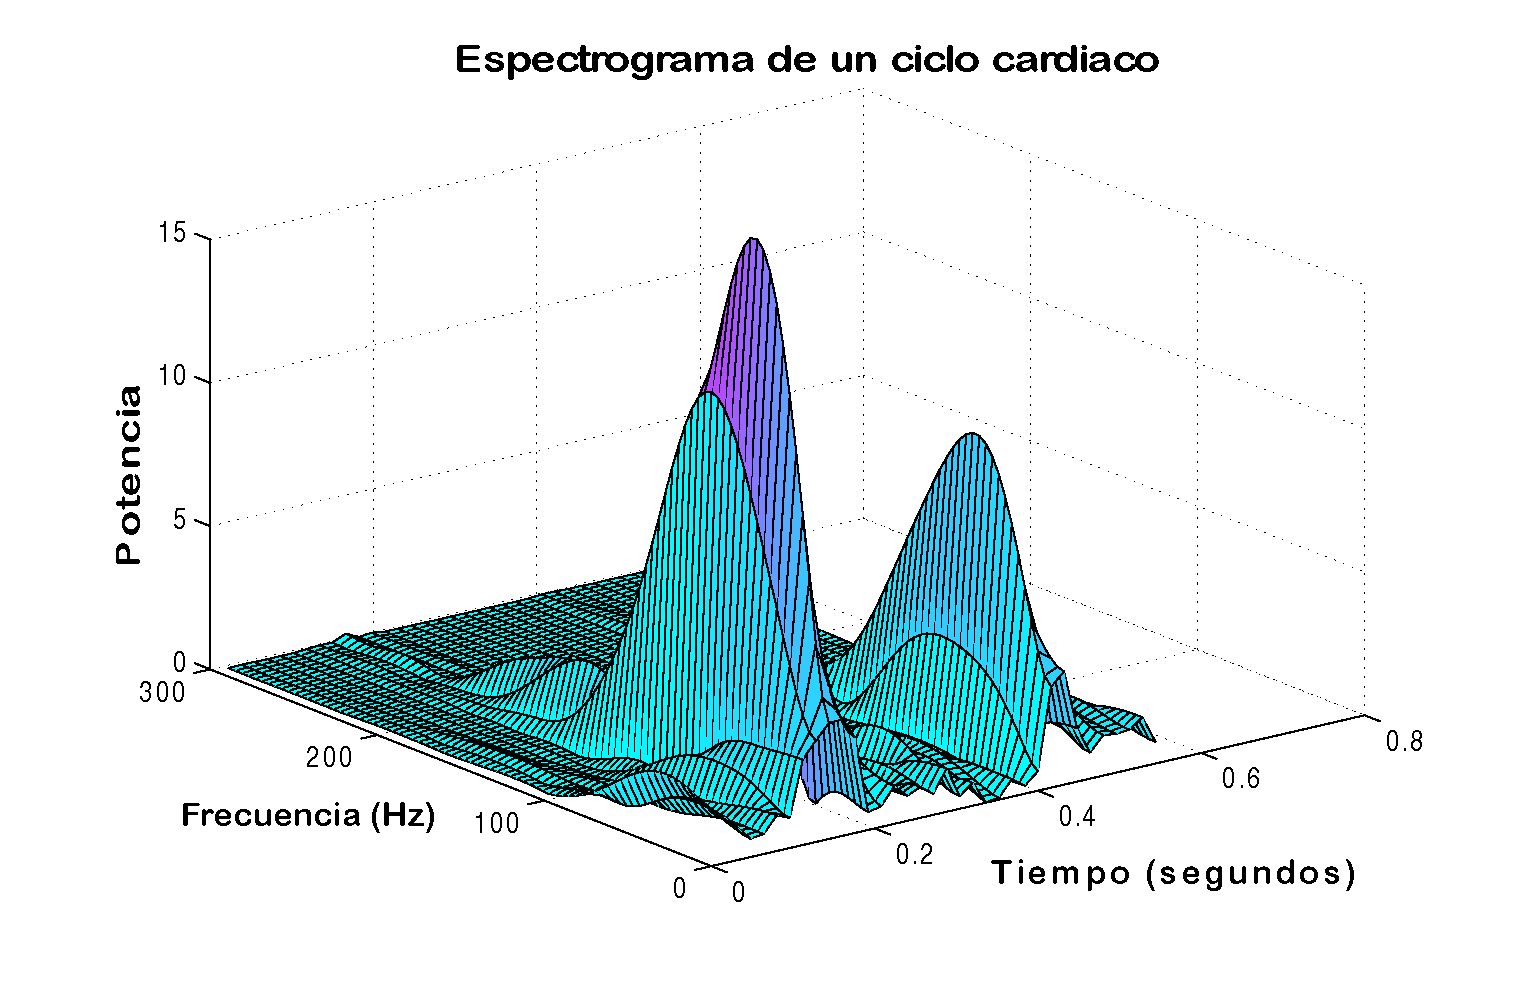
\includegraphics[scale = 0.48]{spectrogram_PCG.eps}
\end{center}
\par
\caption{Espectrograma de un ciclo cardiaco.}
\label{spec_pcg}
\end{figure}
%=======================================

La representación temporal de la envolvente de los sonidos cardiacos así como su contenido frecuencial permite identificar correctamente si se trata de eventos normales, como los que hemos mencionado en esta sección. Estos sonidos también garantizarán un funcionamiento mecánico adecuado del corazón, esto es, válvulas cardíacas trabajando adecuadamente. 

\section{Patologías cardiacas}
Las válvulas o valvas cardiacas son compuertas encargadas de regular el flujo sanguíneo a través de las aurículas y ventrículos del corazón, es por ello que la principal fuente de sonidos cardiacos anormales o patologías detectadas son daños en alguna(s) de éstas. Se distinguen principalmente dos tipos de daños valvulares en cuanto a su funcionamiento \cite{Leatham1987}. 

Particularmente son las válvulas cardiacas izquierdas las que pueden fallar al no abrir apropiadamente, a esta anomalía se le conoce como \emph{estenosis}. Por otra parte, cuando las valvas no puedan cerrar de manera adecuada se les denominará \emph{incompetentes}, provocando un bajo flujo sanguíneo o \emph{regurgitación} \cite[]{Abbas2009}. 

Los daños valvulares mencionados anteriormente producen un flujo turbulento del torrente sanguíneo a través del corazón, el cual presenta un comportamiento más brusco y puede ser percibido de manera auditiva \cite[]{koymen87}. En efecto, esto se traduce a que el PCG de una patología o anomalía cardiaca presenta cambios a frecuencias más elevadas y tiempos más cortos, teniendo alteraciones en la forma de onda y desde luego en el espectrograma. La Figura \ref{soplo_diastolico} muestra la forma de onda de una señal patológica producto de un soplo diastólico, evento que se observa entre S1 y S2 presentando a diferencia de éstos una frecuencia no tan consistente y una duración temporal mayor.
%================================
\begin{figure}[ht]
\begin{center}
\includegraphics[scale = 0.45]
{diastolic_rumble.eps}
\end{center}
\par
\caption{Forma de onda de un soplo diastólico.}
\label{soplo_diastolico}
\end{figure}
%=======================================
\section{Codificación de audio}
El sonido es un fenómeno dado por la propagación de ondas mecánicas a través de un medio, que generalmente es el aire en nuestro caso. Cualquier sonido tiene características analógicas por naturaleza, esto dado que por medio de nuestro sistema auditivo tenemos la capacidad en efecto de escuchar un sonido de manera continua \cite[]{Painter2000,Bosi2003}. 

Sin embargo, el empleo y demanda de sistemas digitales en la actualidad crea la necesidad de reproducir, transmitir, procesar y grabar al sonido digitalmente. Un \emph{códec} (codificador-decodificador) es un dispositivo que toma las señales analógicas de audio como entrada y las transforma temporalmente en una representación digital\footnote{Es decir, una cantidad adecuada (limitada) de bits para poder almacenar y representar una señal de audio.} conveniente para realizar las tareas antes mencionadas \cite[]{Bosi2003}. 

En el caso de este trabajo de tesis se requiere transmitir y almacenar señales de audio cardiaco, las cuales son producto de un fenómeno continuo y por lo tanto analógicas por naturaleza. El canal de almacenamiento y/o transmisión es limitado, la baja tasa de datos disponible hace necesaria una compresión y codificación eficiente de la señal del fonocardiograma. 

La Figura \ref{diag_codec} muestra la funcionalidad que tendrá el códec adaptado a audio cardiaco que se presenta en este documento.

%================================
\begin{figure}[ht]
\begin{center}
\includegraphics[scale = 0.46]
{diag_codec1.png}
\end{center}
\par
\caption{Esquema general del codificador-decodificador diseñado para audio cardiaco.}
\label{diag_codec}
\end{figure}
%=======================================


La codificación de audio es un proceso que requiere la digitalización de una forma de onda completamente analógica, para ello la señal deberá de sufrir diferentes procesos \cite[]{Jayant1974}. 

En la Figura \ref{dig_signal} se muestra una ilustración cualitativa de cómo una forma de onda análoga, la cual es \emph{continua} en tiempo y en amplitud es transformada al dominio digital. 

El proceso comienza con la discretización en tiempo, lo cual es conocido como \emph{muestreo}. Posteriormente se realiza la discretización en amplitud, a lo cual se le denomina \emph{cuantificación}. 

La forma de onda mostrada en la Figura \ref{dig_signal}  de la parte a) es análoga, y hasta completar el proceso en la parte d) puede apreciarse la versión digitalizada de la misma. Cada una de las muestras de la forma de onda en tiempo mostradas en d) tiene un número finito de valores de amplitud y tiempo permisibles.

La transformación de a) hacia d) puede ser por medio del paso c) y posteriormente el d) generalmente, es decir, primero se muestrea a la señal y posteriormente se cuantifica. Es importante verificar la resolución en la realización de los procedimientos anteriores, pues en efecto la señal perderá calidad y en especial durante la cuantificación, que en efecto es un proceso de compresión con pérdidas. Durante el muestreo es importante respetar el parámetro de \emph{frecuencia de muestreo} para una adecuada representación de la señal.

%================================
\begin{figure}[ht]
\begin{center}
\includegraphics[width= 6.5in]
{dig_signal.eps}
\end{center}
\par
\caption{Cuatro tipos de señales: a) Continua en amplitud y tiempo (analógica); b) discreta en amplitud y continua en tiempo; c) continua en amplitud y discreta en tiempo; d) discreta en tiempo y amplitud.}
\label{dig_signal}
\end{figure}
%=======================================


\subsection{La psicoacústica en el modelado y codificación de audio}

El diseño de los algoritmos de codificación está basado en las características del receptor, con lo cual se garantizará una optimización en la eficiencia y calidad del código. En el caso del audio el receptor es el oído humano, cuya percepción se ve afectada por sus propiedades de \emph{enmascaramiento sonoro} \footnote{Fenómeno que ocurre cuando dos o más sonidos son reproducidos simultáneamente. El más débil de ellos resultará inaudible.}. Por medio de la \emph{psicoacústica} se realiza la caracterización adecuada del sistema de percepción auditiva humana y particularmente el análisis de las capacidades tiempo-frecuencia del oído interno \cite[]{Painter2000}.

Aplicar principios de percepción del oído para la codificación de audio es realmente relevante para diversos codificadores, algunos explotan el hecho de descartar información que no es detectable para cualquier oyente bien entrenado y así comprimir la señal \cite[]{Schroeder1979}. Esta información irrelevante se identifica durante el análisis de señal incorporando en el codificador principios psicoacústicos como umbrales absolutos de audición, análisis de bandas de frecuencia críticas, enmascaramiento simultáneo y temporal, entre otros. 

El umbral absoluto de audición caracteriza la cantidad de energía necesaria en un tono puro tal que pueda ser detectado por un oyente en un ambiente sin ruido. La \mbox{Figura \ref{umbral_audicion}} muestra el comportamiento del umbral de audición absoluto en el espectro frecuencial. Dicha gráfica es el resultado de cuantificar el nivel de presión de sonido (SPL) requerido para cada frecuencia detectada por el oyente (tono puro).
%================================
\begin{figure}[ht]
\begin{center}
\includegraphics[scale = 0.86]
{umbral_audicion.pdf}
\end{center}
\par
\caption{Umbral absoluto de audición. Tomado de \cite{Painter2000}.}
\label{umbral_audicion}
\end{figure}
%=======================================

\subsection{El códec de audio}
Como mencionamos anteriormente un códec de audio es el sistema que incluye el conjunto de algoritmos para permitir codificar y decodificar datos auditivos en una cantidad limitada de bits \cite[]{Bosi2003,Painter2000}. Es importante que un códec pueda comprimir el archivo de audio para ocupar el menor espacio posible y una calidad aceptable para reproducirlo adecuadamente \cite[]{Painter2000}. Los siguientes parámetros son importantes en la definición de un códec de audio:
\begin{itemize}
	\item\textbf{Número de canales.} Esto se refiere al número de señales simultáneas de audio que contiene el flujo de datos. De acuerdo a ello la señal puede ser mono (un canal), estéreo (dos canales) o multicanal 5.1 (6 canales) ó 7.1 (8 canales).
	\item\textbf{Frecuencia de muestreo.} Una señal analógica de audio necesita ser discretizada primeramente en el tiempo, para ello se emplea el muestreo. El teorema de Nyquist establece que la frecuencia de muestreo adecuada para representar una señal debe ser el doble de la frecuencia máxima contenida en el ancho de banda de la señal. Ejemplos de ello son los estándares MPEG-3 (MP3), el cual muestrea con calidad de CD a diferentes frecuencias de muestreo; la más común es de 44,100 Hz teniendo en cuenta que el oído humano no es capaz de escuchar frecuencias superiores a 22 kHz.
	\item\textbf{Número de bits por muestra.} Con ello se determina qué precisión existe al reproducir la señal original así como el rango dinámico de la misma. Suelen utilizarse en los codificadores convencionales 8, 16 ó 24 bits por muestra aunque en calidad CD comúnmente se emplean 16. 
	\item\textbf{Tipo de compresión.} Se distingue entre compresión con pérdidas (\emph{lossy compression}) y sin pérdidas (\emph{lossless compression}).
		\begin{itemize}
		\item \emph{Compresión con pérdidas}: La información que se considera irrelevante es despreciada, aunque con ello es evidente 					tener una pérdida en la calidad del resultado al ejecutar la decodificación final.		
		\item \emph{Compresión sin pérdidas}: Toda la información es transmitida, sólo se elimina la información repetida o redundante y la 								información que no se repite se almacena ocupando un menor espacio.
		\end{itemize}
		
	\item\textbf{Tasa de bits (datos).} Esta cantidad determina el número de bits necesarios por unidad de tiempo y no puede deducirse a través de los parámetros anteriores, ya que pudo aplicarse una compresión con o sin pérdidas. De acuerdo a su estabilidad puede ser \emph{constante (CBR)} o \emph{variable (VBR)}. VBR es de uso más frecuente en audio y además más eficiente que CBR ya que existen tramos de silencios aleatorios donde deberá bajar la cantidad de bits a transmitir y por lo tanto variar la tasa. 
		\begin{itemize}
		\item\emph{Tasa de bits constante (CBR)}: La tasa de salida del codificador es constante. CBR es útil en en flujo de datos multimedia para canales de capacidad limitada, sin embargo no es la mejor opción para almacenamiento, ya que no asigna suficientes bits para las secciones complejas (por lo tanto se degrada la calidad) además de usar bits innecesarios en secciones de menor complejidad.
		\item\emph{Tasa de bits variable (VBR)}: En este método de compresión se consigue una mayor calidad de sonido para un tamaño de archivo determinado. En contraste a CBR se otorga la tasa de bits necesaria a cada parte del archivo que se pretende codificar consiguiendo una calidad mayor en archivos de tamaño reducido. Al codificar con VBR, el codificador asignará las tasas de bits que variarán según la complejidad de la onda de audio a lo largo del archivo. Este formato es muy apropiado para la transmisión de audio en tiempo real.
		\end{itemize}
\end{itemize}
En la actualidad existen diversos códecs de audio, aunque cada vez son más complejos y presentan características adicionales a las mencionadas anteriormente. De acuerdo a los parámetros existentes en algunos codificadores de audio expuestos por \cite{Bosi2003}, se ha realizado en esta tesis una clasificación en cuatro grandes grupos:
\begin{itemize} 
	\item \textbf{Codificadores de forma de onda.} Estos codificadores están basados en el estudio general de la señal, de tal manera que intentan reproducir la forma de la señal de entrada \cite[]{OReilly1984}. Son diseñados en general para ser independientes de la señal, de manera que puedan ser útiles para  codificar una variedad extensa de señales; la redundancia de la señal es aprovechada para lograr una compresión. 
		
	Algunos codificadores de forma de onda son:			
	\begin{itemize}
				\item Modulación por codificación de pulsos (\emph{Pulse Code Modulation} ó PCM). Esta codificación es la base para la 						mayoría de los codificadores y a la vez se incluye en el procedimiento para digitalizar una señal. Basta con 							representar mediante impulsos las variaciones en amplitud de las muestras de la señal de entrada.
				\item Modulación diferencial por pulsos codificados (DPCM). Basándose en el principio de PCM, DPCM codifica solamente la 						diferencia entre la muestra presente y la muestra anterior de la señal de entrada. Se envía una cantidad mayor de 						información y un número más reducido de bits si se compara con PCM, sin embargo si existe un error en alguna 						trama codificada con PCM éste afectará tanto a la muestra actual y las muestras subsecuentes.
				\item Modulación diferencial adaptativa por pulsos codificados (ADPCM). Se trata de una variante de DPCM donde se varía la 					escala de codificación según las diferencias entre las muestras actual y subsecuente, es decir se asignan cantidades 						variables de bits a éstas según corresponda.
			\end{itemize}
Algunos codificadores de forma de onda basados en PCM u otras de sus variantes han tenido éxito para transmitir señales de voz sobre canales telefónicos. Ejemplos de éstos son el codificador $\mu-255 PCM$ \cite[]{Dammann1972} y el $G722$ \mbox{\cite[]{Mermelstein1988}}.  

	\item \textbf{Codificadores perceptuales.} Se aprovechan las limitaciones en la percepción del sistema auditivo humano para codificar el flujo de datos. Las muestras son codificadas en formato PCM y son convertidas al dominio de la frecuencia. Dada esta conversión la señal puede descomponerse en sub-bandas y proporcionar una resolución mayor a las bandas de frecuencia donde el oído humano sea más sensible. 
	La codificación puede también llevarse a cabo por transformada, codificando las componentes de una transformada unitaria de la señal realizando la operación inversa (antitransformada o transformada inversa) en el decodificador. En este caso la compresión se presenta debido a lo no correlacionadas que tienden a ser las componentes generadas por las transformadas unitarias de manera que pueden codificarse independientemente.
Otra manera útil de desechar información irrelevante al codificar audio de manera perceptual es la codificación en \emph{sub-bandas}, pasando la señal de audio por diversos filtros pasa-banda a diferentes frecuencias para codificarla de manera independiente y dar diferente resolución a las bandas más sensibles.

Se muestra en la Figura \ref{cod_perceptual} el diagrama a bloques que ilustra el procedimiento de codificación de audio de manera perceptual.
%================================
\begin{figure}[ht]
\begin{center}
\includegraphics[scale = 0.66]
{diagCodPerceptual.pdf}
\end{center}
\par
\caption{Diagrama a bloques de un codificador de audio perceptual.}
\label{cod_perceptual}
\end{figure}
%=======================================

El grupo de trabajo \textbf{Moving Picture Experts Group (MPEG)} ha establecido diversos estándares para la transmisión de audio, aprovechando en ellos la codificación perceptual para diseñar codificadores como MP3 \cite[]{Musmann2006,Noll1997}. Otro codificador perceptual de audio que ha tenido reconocimiento en el mercado es el \emph{Advanced Audio Coding (AAC)} \cite[]{Bosi1997}.

	\item \textbf{Codificadores paramétricos.} Estos codificadores se basan en el hecho de que el audio y la voz pueden representarse y sintetizarse como tonos aislados o patrones armónicos, esto es, representarlos con ondas senoidales y componentes ruidosas (\emph{sinusoid plus noise modeling}). Los parámetros de las sinusoides son los que se codifican: amplitud, frecuencia fundamental o componentes espectrales. Estos parámetros requieren por lo general pocos bits para ser representados \cite[]{Quatieri1985,McAulay1986,RuizReyes2010}. 
	
	En la Figura \label{cod_parametrico} se muestra el diagrama a bloques de un codificador de audio tipo paramétrico.
		%================================
		\begin{figure}[ht]
		\begin{center}
		\includegraphics[scale = 0.66]
			{diagCodParametrico.pdf}
		\end{center}
		\par
		\caption{Diagrama a bloques de un codificador de audio paramétrico.}
		\label{cod_parametrico}
		\end{figure}
		%=======================================
	\item \textbf{Codificadores híbridos.}  Combinan las técnicas de los codificadores de forma de onda para obtener la 				señal de audio de más alta calidad con tasas bajas de bits. Un conjunto de muestras es analizado como si se tratase de una sola 				para obtener los parámetros de la señal. Cuando la trama se decodifica los parámetros son sintetizados para conseguir que se 				parezca al original. Se conocen algunos codificadores híbridos de la literatura:
		\begin{itemize}
			\item El vocoder (codificador de voz) basado en la técnica \emph{Residual-Excited Linear Prediction (RELP)} desarrollado por 						\cite{Un1975}.
			\item Algunos codificadores de voz basados en el algoritmo \emph{Code Excited Linear Prediction (CELP)}, donde se emplean diccionarios o bloques de código adaptativos \cite[]{Mano1995,Kipper1991,Miki1994,Koishida1996}.
			\item Codificadores que emplean predicción lineal mediante suma de vectores, conocidos como\emph{Vector Sum Excited Linear Prediction (VSELP)}. Algunos de ellos han sido desarrollados por \cite{Gu1995,Sunwoo1991,Choi1996,Gerson1990}.
			\item Codificación mediante el método \emph{Regular Pulse Excitation-Long Term Prediction (RPE-LTP)}. Los codificadores diseñados por \cite{Huerta2001a,McLoughlin2000,Coleman1989} se basan en esta técnica. 
		\end{itemize}	
\end{itemize}

En este trabajo de tesis se desarrollará un codificador tipo \emph{paramétrico} con pérdidas aprovechando la alta correlación existente entre los eventos del audio cardiaco y las formas de onda conocidas como átomos de Gabor. La siguiente sección describe las técnicas que se han usado en la literatura para el modelado del fonocardiograma.

\section{Estado del arte en el modelado de sonidos cardiacos}
La primer parte para el diseño de un codificador de audio cardiaco paramétrico consiste en el modelado matemático, el cual dotará de características propias y codificables al PCG además de encontrar la representación más adecuada y que represente mayor compresión. 
Robert Hooke, conocido por sus trabajos en elasticidad de materiales, otorgó potencialidad en el diagnóstico de patologías a la auscultación cardiaca \cite[]{Wood1995}. Y es que Hooke fue capaz de escuchar claramente los sonidos pertenecientes a los latidos del corazón y planteaba que tal vez pudiese indagar sobre el funcionamiento de otros órganos del cuerpo humano mediante el sonido que éstos generaban \cite[]{Leatham1987}.

El estetoscopio fue creado por Laënnec en 1816 \cite[]{Roguin2006} e hizo del fonocardiograma una herramienta fundamental en la diagnosis clínica hasta nuestros días. Sin embargo, la escasez de estándares en la nomenclatura, los transductores empleados en el registro y las locaciones para llevarlo a cabo mostraron un progreso lento; como resultado se tuvo un pobre entendimiento de los mecanismos del sonido cardiaco y la inherente complejidad de los sonidos cardiacos. 

Sin embargo, algunos factores han hecho del PCG una herramienta de diagnóstico limitada. La percepción auditiva humana es la primer limitante; aunque los especialistas y cardiólogos muestren singulares habilidades en el reconocimiento de diversas patologías no se garantiza que la auscultación tenga una precisión para diagnosticar. En efecto, toda señal de audio es pasa-bajas, de baja intensidad para el oído humano y muy corta duración. La banda baja de frecuencias puede concentrar también información importante del fonocardiograma.
 
 Los avances en el procesamiento digital de señales así como la aparición del diagnóstico asistido por computadora (\emph{Computer-Aided Diagnosis}) han logrado reforzar al PCG para ser una herramienta importante en el estudio de anomalías cardiacas. Los estetoscopios actuales muestran ahora las formas de onda y el análisis de la señal es más extenso \cite[]{Mahnke2009,Watrous2008}.
 
 Algunos trabajos en la literatura han realizado un análisis extenso en el plano tiempo-frecuencia del PCG, mostrando una caracterización espectral del mismo ya sea por espectrogramas calculados por la STFT o distribuciones Wigner-Ville \cite[]{Ghofrani1993}, tal es el caso de \cite{Djebbari2000,Debbal2007,Debbal2008} y \cite{Jasper2010}. En otros trabajos como los realizados por \cite{Boutana2011} y \cite{DEBBAL2006} se realiza la identificación de cardiopatologías usando como herramientas las distribuciones tiempo-frecuencia antes mencionadas.
 
 De acuerdo a lo mencionado en las secciones anteriores de este trabajo con respecto al PCG se trata de una señal no estacionaria, esto es, los ciclos cardiacos no son consistentes en posición, duración temporal ni contenido frecuencial. Dada esta característica los autores se han dedicado a analizar las componentes principales por separado: los primeros eventos cardiacos (S1) son estudiados en los trabajos de \cite{Chen1997,Wood1995} y \cite{Wood1992}, mientras que los trabajos de \cite{Hedayioglu2012,wang04} han estudiado de manera específica el comportamiento del evento S2.
 
 Se ha propuesto en el trabajo de \cite{koymen87} un modelado del PCG a partir de sinusoides amortiguadas, dadas que las estructuras en el pecho (lugar donde se realiza la auscultación) y venas de mayor contribución constituyen un sistema selectivo en frecuencia excitado por la aceleración y desaceleración de las válvulas. 
 
 El modelado del fonocardiograma mediante senoidales amortiguadas se ha extendido en la literatura para realizar diversos procesos en el PCG tales como eliminación de ruido (\emph{denoising}), segmentación de eventos, separación de componentes (diagnóstico de cardiopatologías así como la división de los eventos S1 y S2) y escalamiento en el plano tiempo-frecuencia \cite[]{Nieblas2013,Zhang1998b,Zhang1998a,Sava1998}.
 
  Los trabajos anteriormente citados emplean el algoritmo \mbox{\textbf{Matching Pursuit}} \cite[]{Mallat1993} con éxito en el análisis y síntesis del fonocardiograma, tal método selecciona un conjunto de formas de onda cosenoidales (cuyo \emph{amortiguamiento} viene dado por la modulación mediante una ventana gaussiana) denominadas \emph{átomos de Gabor} pertenecientes a un bloque conocido como diccionario. 
   
 La compresión de fonocardiogramas es el paso donde se extraen los parámetros más importantes del modelado de señal para representarlos de manera digital. Otros autores de la literatura han realizado este procedimiento efectuando la representación del audio cardiaco mendiante ondeletas (en Inglés \emph{wavelets}) como \cite{Alajarin2004,Alajarin2005,Martinez-Alajarin2006}, además de realizar también por el mismo método el proceso de \emph{de-noising} \cite[]{Messer2001}. 
 
 Por otra parte, en la tesis desarrollada por \cite{castorena2012} se propone adaptar códecs ya existentes para trasmitir el audio cardiaco sobre diversos escenarios que involucran redes con bajas tasas de datos. Posteriormente \cite{Nieblas2014} analizó diversos bloques de ondeletas mediante Matching Pursuit para elegir el que represente a la señal PCG de la manera más adecuada. 
 
 No obstante, hasta el momento no se conoce que se haya diseñado algún codificador de audio cardiaco, se ha revisado en esta sección que el modelado y la compresión del PCG han sido explorados quedando pendiente la realización de un códec que permita describir en bajas tasas de datos a esta señal para su transmisión en redes de bajos recursos.
 
  En el siguiente capítulo se aplicará la compresión de fonocardiogramas mediante \mbox{\textbf{Matching Pursuit}}, ya que conforma una parte medular del codificador a diseñar en esta tesis.
  

} }%
%BeginExpansion
\chapter{La señal de fonocardiograma}\label{capit:cap2}
\vspace{-2.0325ex}%
\noindent
\rule{\textwidth}{0.5pt}
\vspace{-5.5ex}% 
\newcommand{\pushline}{\Indp}% Indent puede ir o no :p



En este capítulo se conocerán las características fisiológicas del audio cardiaco, comprendiendo lo que representan cada uno de los sonidos generados así como su clasificación. De igual manera se expondrá una descripción del fonocardiograma como señal eléctrica y algunos parámetros importantes de la misma que servirán en su procesamiento digital, como la respuesta en frecuencia y forma de onda temporal. Se definirán también en esta sección las características de los sonidos que representen algún mal o anomalía en el funcionamiento del corazón, qué parámetros las caracterizan así como algunas consideraciones en su tratamiento como señal eléctrica y acústica. 

El codificador de fonocardiograma (al cual denotaremos como PCG por sus siglas en inglés) involucra diversos procedimientos en su realización. Es importante por lo tanto, conocer las características y parámetros de algunos códecs existentes; debido a esto se ha incluido en este capítulo una breve introducción a la codificación de audio en general.

De igual manera se mostrará en esta sección un breve panorama o \emph{estado del arte} en codificación de sonidos cardiacos, basado en los trabajos realizados en la literatura para el modelado y procesamiento de fonocardiogramas. Se tomarán algunas consideraciones importantes sobre estos trabajos y se definirá cuáles se han empleado en esta tesis para el desarrollo del códec.

\section{Origen fisiológico y representación de los sonidos cardiacos}

Como se ha definido anteriormente un fonocardiograma representa al audio cardiaco; se trata de una señal mecánica sonora tomada con un dispositivo médico llamado estetoscopio. Los sonidos generados por esta señal describen el comportamiento o acción mecánica de las válvulas o valvas del corazón, las cuales son compuertas que abren o cierran sistemáticamente para dar paso a la regulación de la sangre a través de las venas y arterias \cite[]{Abbas2009}. 

Existen cuatro válvulas, cada una asociada a las principales venas que están conectadas al órgano cardiaco: válvula aórtica, válvula pulmonar, válvula mitral y válvula tricúspide. Estos componentes se muestran en la Figura \ref{valvulas}.

%================================
\begin{figure}[ht]
\begin{center}
\includegraphics[width=3.3in]
{valvulas_cardiacas.jpg}
\end{center}
\par
\caption{Localización de las válvulas cardiacas. 
Tomado de \protect\url{http://www.nlm.nih.gov/medlineplus/spanish/ency/esp_imagepages/9380.htm}}
\label{valvulas}
\end{figure}
%=======================================

Son dos eventos importantes los que constituyen un PCG ordinario, denominados como S1 y S2. En el caso del primer evento o S1 se tiene un sonido que describe la actividad dada por la apertura de las válvulas aórtica y pulmonar y el cierre de las válvulas mitral y tricúspide (esto evita que la sangre circule hacia esta sección). En este evento se completa una \textbf{sístole ventricular}, donde las ventrículos se contraen para expulsar la sangre hacia las arterias \cite[]{Djebbari2000}.

El segundo evento cardiaco S2 describe el complemento de los acontecimientos dados en S1, esto es, las válvulas mitral y tricúspide ahora se abren para recibir la sangre mientras que los conductos aórtico y pulmonar se han cerrado. Este proceso se denomina \textbf{sístole aurícular} y en efecto, ahora son las aurículas quienes se han contraído para expulsar la sangre hacia los ventrículos. Se denomina \emph{ciclo cardiaco} cuando secuencialmente han ocurrido los sonidos S1 y S2. La \textbf{diástole} ocurre después de completarse un ciclo cardiaco y se trata de un periodo donde se relajan las aurículas y ventrículos. Estos dos sonidos son identificados en un fonocardiograma regular durante la actividad de un ciclo \cite[]{Abbas2009}. 
 
Existen otros dos sonidos cardiacos: S3 y S4, los cuales son asociados a otros eventos y generalmente son despreciados en el análisis del PCG. En el caso del llenado o asimilación de sangre hacia los ventrículos se origina S3, mientras que S4 ocurre al final de la diástole surgido por la contracción de las aurículas cuando han desplazado el flujo de los ventrículos \cite[]{koymen87}. 

Al espacio donde no ocurre algún evento cardiaco se le denomina \emph{silencio}.  

\section{Características del fonocardiograma}
Como señal eléctrica un fonocardiograma consta de formas de onda específicas asociadas a los sonidos cardíacos que se mencionaron anteriormente (S1 y S2). Los eventos cardíacos preservan cierta duración en tiempo y por lo tanto también contienen cierto intervalo de frecuencias, características que se muestran en la Tabla \ref{sonidosCardiacosNormales}. En la Figura \ref{ciclo} puede observarse la forma de onda de los ruidos o eventos cardiacos normales que constituyen un ciclo cardiaco. 
\begin{table}[h] 
\par
\begin{center}
\begin{tabular}{|c|c|c|}
   \hline 
   Ruido & Duración (s) & Contenido frecuencial (Hz) \\ \hline
   S1      &  0.1-0.12     & 20-150			\\ \hline
   S2      &  0.08-0.12   & 50-60			          \\ \hline
   S3      &  0.04-0.05     & 20-50			\\ \hline
   S4      &  0.04-0.05     & $<$25			\\ \hline
   \hline
   \end{tabular}
   \end{center}
   \caption{Duración y contenido frecuencial de los principales ruidos cardiacos. Tomado de \cite{castorena2012}}
   \label{sonidosCardiacosNormales}   
\end{table}

%================================
\begin{figure}[ht]
\begin{center}
\includegraphics[width=4.3in]
{ciclo_cardiaco.eps}
\end{center}
\par
\caption{Forma de onda de un ciclo cardiaco.}
\label{ciclo}
\end{figure}
%=======================================

Los sonidos cardiacos presentan cambios rápidos con respecto al tiempo y a la frecuencia debido al comportamiento no estacionario de la señal PCG. Es por esto que el estudio y entendimiento de sus características se realiza en un plano conjunto tiempo-frecuencia. La STFT\footnote{Transformada de Fourier de Tiempo Corto \emph{(Short Time Fourier Transform)}.} es una herramienta propicia para el análisis en los cambios del comportamiento del fonocardiograma \cite[]{Djebbari2000}. 

En la Figura \ref{spec_pcg} se muestra el espectrograma (gráfica de la STFT) de un ciclo cardiaco, con el cual se observa la evolución tiempo-frecuencia de los eventos S1 y S2 además de su contenido frecuencial ya antes definido. 
%================================
\begin{figure}[ht]
\begin{center}
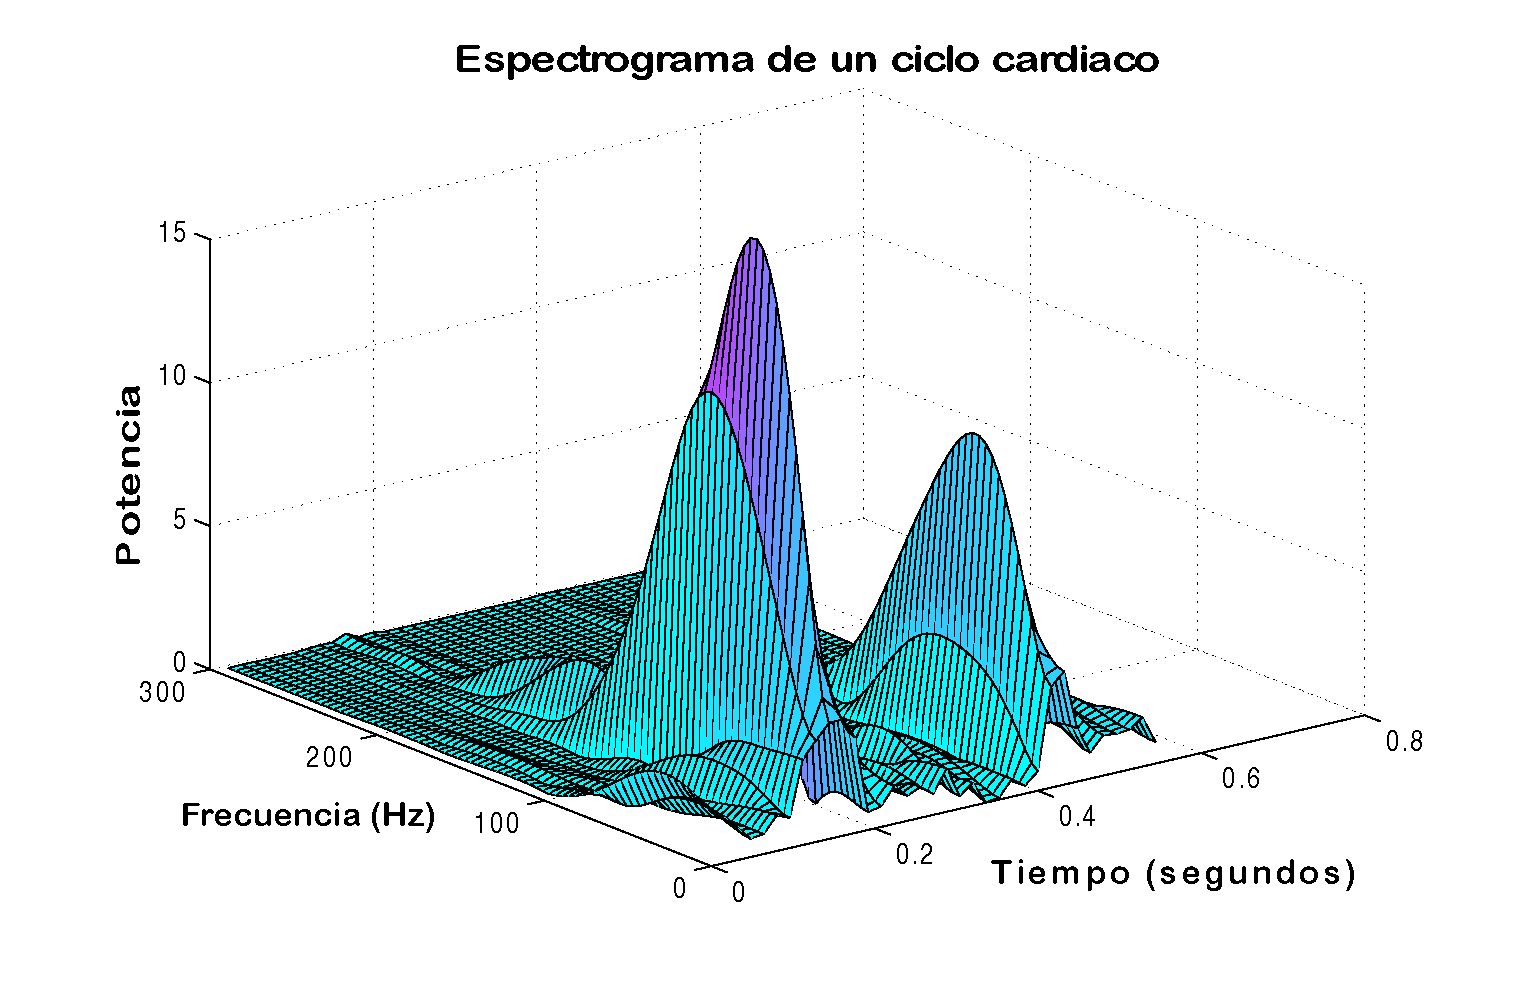
\includegraphics[scale = 0.48]{spectrogram_PCG.eps}
\end{center}
\par
\caption{Espectrograma de un ciclo cardiaco.}
\label{spec_pcg}
\end{figure}
%=======================================

La representación temporal de la envolvente de los sonidos cardiacos así como su contenido frecuencial permite identificar correctamente si se trata de eventos normales, como los que hemos mencionado en esta sección. Estos sonidos también garantizarán un funcionamiento mecánico adecuado del corazón, esto es, válvulas cardíacas trabajando adecuadamente. 

\section{Patologías cardiacas}
Las válvulas o valvas cardiacas son compuertas encargadas de regular el flujo sanguíneo a través de las aurículas y ventrículos del corazón, es por ello que la principal fuente de sonidos cardiacos anormales o patologías detectadas son daños en alguna(s) de éstas. Se distinguen principalmente dos tipos de daños valvulares en cuanto a su funcionamiento \cite{Leatham1987}. 

Particularmente son las válvulas cardiacas izquierdas las que pueden fallar al no abrir apropiadamente, a esta anomalía se le conoce como \emph{estenosis}. Por otra parte, cuando las valvas no puedan cerrar de manera adecuada se les denominará \emph{incompetentes}, provocando un bajo flujo sanguíneo o \emph{regurgitación} \cite[]{Abbas2009}. 

Los daños valvulares mencionados anteriormente producen un flujo turbulento del torrente sanguíneo a través del corazón, el cual presenta un comportamiento más brusco y puede ser percibido de manera auditiva \cite[]{koymen87}. En efecto, esto se traduce a que el PCG de una patología o anomalía cardiaca presenta cambios a frecuencias más elevadas y tiempos más cortos, teniendo alteraciones en la forma de onda y desde luego en el espectrograma. La Figura \ref{soplo_diastolico} muestra la forma de onda de una señal patológica producto de un soplo diastólico, evento que se observa entre S1 y S2 presentando a diferencia de éstos una frecuencia no tan consistente y una duración temporal mayor.
%================================
\begin{figure}[ht]
\begin{center}
\includegraphics[scale = 0.45]
{diastolic_rumble.eps}
\end{center}
\par
\caption{Forma de onda de un soplo diastólico.}
\label{soplo_diastolico}
\end{figure}
%=======================================
\section{Codificación de audio}
El sonido es un fenómeno dado por la propagación de ondas mecánicas a través de un medio, que generalmente es el aire en nuestro caso. Cualquier sonido tiene características analógicas por naturaleza, esto dado que por medio de nuestro sistema auditivo tenemos la capacidad en efecto de escuchar un sonido de manera continua \cite[]{Painter2000,Bosi2003}. 

Sin embargo, el empleo y demanda de sistemas digitales en la actualidad crea la necesidad de reproducir, transmitir, procesar y grabar al sonido digitalmente. Un \emph{códec} (codificador-decodificador) es un dispositivo que toma las señales analógicas de audio como entrada y las transforma temporalmente en una representación digital\footnote{Es decir, una cantidad adecuada (limitada) de bits para poder almacenar y representar una señal de audio.} conveniente para realizar las tareas antes mencionadas \cite[]{Bosi2003}. 

En el caso de este trabajo de tesis se requiere transmitir y almacenar señales de audio cardiaco, las cuales son producto de un fenómeno continuo y por lo tanto analógicas por naturaleza. El canal de almacenamiento y/o transmisión es limitado, la baja tasa de datos disponible hace necesaria una compresión y codificación eficiente de la señal del fonocardiograma. 

La Figura \ref{diag_codec} muestra la funcionalidad que tendrá el códec adaptado a audio cardiaco que se presenta en este documento.

%================================
\begin{figure}[ht]
\begin{center}
\includegraphics[scale = 0.46]
{diag_codec1.png}
\end{center}
\par
\caption{Esquema general del codificador-decodificador diseñado para audio cardiaco.}
\label{diag_codec}
\end{figure}
%=======================================


La codificación de audio es un proceso que requiere la digitalización de una forma de onda completamente analógica, para ello la señal deberá de sufrir diferentes procesos \cite[]{Jayant1974}. 

En la Figura \ref{dig_signal} se muestra una ilustración cualitativa de cómo una forma de onda análoga, la cual es \emph{continua} en tiempo y en amplitud es transformada al dominio digital. 

El proceso comienza con la discretización en tiempo, lo cual es conocido como \emph{muestreo}. Posteriormente se realiza la discretización en amplitud, a lo cual se le denomina \emph{cuantificación}. 

La forma de onda mostrada en la Figura \ref{dig_signal}  de la parte a) es análoga, y hasta completar el proceso en la parte d) puede apreciarse la versión digitalizada de la misma. Cada una de las muestras de la forma de onda en tiempo mostradas en d) tiene un número finito de valores de amplitud y tiempo permisibles.

La transformación de a) hacia d) puede ser por medio del paso c) y posteriormente el d) generalmente, es decir, primero se muestrea a la señal y posteriormente se cuantifica. Es importante verificar la resolución en la realización de los procedimientos anteriores, pues en efecto la señal perderá calidad y en especial durante la cuantificación, que en efecto es un proceso de compresión con pérdidas. Durante el muestreo es importante respetar el parámetro de \emph{frecuencia de muestreo} para una adecuada representación de la señal.

%================================
\begin{figure}[ht]
\begin{center}
\includegraphics[width= 6.5in]
{dig_signal.eps}
\end{center}
\par
\caption{Cuatro tipos de señales: a) Continua en amplitud y tiempo (analógica); b) discreta en amplitud y continua en tiempo; c) continua en amplitud y discreta en tiempo; d) discreta en tiempo y amplitud.}
\label{dig_signal}
\end{figure}
%=======================================


\subsection{La psicoacústica en el modelado y codificación de audio}

El diseño de los algoritmos de codificación está basado en las características del receptor, con lo cual se garantizará una optimización en la eficiencia y calidad del código. En el caso del audio el receptor es el oído humano, cuya percepción se ve afectada por sus propiedades de \emph{enmascaramiento sonoro} \footnote{Fenómeno que ocurre cuando dos o más sonidos son reproducidos simultáneamente. El más débil de ellos resultará inaudible.}. Por medio de la \emph{psicoacústica} se realiza la caracterización adecuada del sistema de percepción auditiva humana y particularmente el análisis de las capacidades tiempo-frecuencia del oído interno \cite[]{Painter2000}.

Aplicar principios de percepción del oído para la codificación de audio es realmente relevante para diversos codificadores, algunos explotan el hecho de descartar información que no es detectable para cualquier oyente bien entrenado y así comprimir la señal \cite[]{Schroeder1979}. Esta información irrelevante se identifica durante el análisis de señal incorporando en el codificador principios psicoacústicos como umbrales absolutos de audición, análisis de bandas de frecuencia críticas, enmascaramiento simultáneo y temporal, entre otros. 

El umbral absoluto de audición caracteriza la cantidad de energía necesaria en un tono puro tal que pueda ser detectado por un oyente en un ambiente sin ruido. La \mbox{Figura \ref{umbral_audicion}} muestra el comportamiento del umbral de audición absoluto en el espectro frecuencial. Dicha gráfica es el resultado de cuantificar el nivel de presión de sonido (SPL) requerido para cada frecuencia detectada por el oyente (tono puro).
%================================
\begin{figure}[ht]
\begin{center}
\includegraphics[scale = 0.86]
{umbral_audicion.pdf}
\end{center}
\par
\caption{Umbral absoluto de audición. Tomado de \cite{Painter2000}.}
\label{umbral_audicion}
\end{figure}
%=======================================

\subsection{El códec de audio}
Como mencionamos anteriormente un códec de audio es el sistema que incluye el conjunto de algoritmos para permitir codificar y decodificar datos auditivos en una cantidad limitada de bits \cite[]{Bosi2003,Painter2000}. Es importante que un códec pueda comprimir el archivo de audio para ocupar el menor espacio posible y una calidad aceptable para reproducirlo adecuadamente \cite[]{Painter2000}. Los siguientes parámetros son importantes en la definición de un códec de audio:
\begin{itemize}
	\item\textbf{Número de canales.} Esto se refiere al número de señales simultáneas de audio que contiene el flujo de datos. De acuerdo a ello la señal puede ser mono (un canal), estéreo (dos canales) o multicanal 5.1 (6 canales) ó 7.1 (8 canales).
	\item\textbf{Frecuencia de muestreo.} Una señal analógica de audio necesita ser discretizada primeramente en el tiempo, para ello se emplea el muestreo. El teorema de Nyquist establece que la frecuencia de muestreo adecuada para representar una señal debe ser el doble de la frecuencia máxima contenida en el ancho de banda de la señal. Ejemplos de ello son los estándares MPEG-3 (MP3), el cual muestrea con calidad de CD a diferentes frecuencias de muestreo; la más común es de 44,100 Hz teniendo en cuenta que el oído humano no es capaz de escuchar frecuencias superiores a 22 kHz.
	\item\textbf{Número de bits por muestra.} Con ello se determina qué precisión existe al reproducir la señal original así como el rango dinámico de la misma. Suelen utilizarse en los codificadores convencionales 8, 16 ó 24 bits por muestra aunque en calidad CD comúnmente se emplean 16. 
	\item\textbf{Tipo de compresión.} Se distingue entre compresión con pérdidas (\emph{lossy compression}) y sin pérdidas (\emph{lossless compression}).
		\begin{itemize}
		\item \emph{Compresión con pérdidas}: La información que se considera irrelevante es despreciada, aunque con ello es evidente 					tener una pérdida en la calidad del resultado al ejecutar la decodificación final.		
		\item \emph{Compresión sin pérdidas}: Toda la información es transmitida, sólo se elimina la información repetida o redundante y la 								información que no se repite se almacena ocupando un menor espacio.
		\end{itemize}
		
	\item\textbf{Tasa de bits (datos).} Esta cantidad determina el número de bits necesarios por unidad de tiempo y no puede deducirse a través de los parámetros anteriores, ya que pudo aplicarse una compresión con o sin pérdidas. De acuerdo a su estabilidad puede ser \emph{constante (CBR)} o \emph{variable (VBR)}. VBR es de uso más frecuente en audio y además más eficiente que CBR ya que existen tramos de silencios aleatorios donde deberá bajar la cantidad de bits a transmitir y por lo tanto variar la tasa. 
		\begin{itemize}
		\item\emph{Tasa de bits constante (CBR)}: La tasa de salida del codificador es constante. CBR es útil en en flujo de datos multimedia para canales de capacidad limitada, sin embargo no es la mejor opción para almacenamiento, ya que no asigna suficientes bits para las secciones complejas (por lo tanto se degrada la calidad) además de usar bits innecesarios en secciones de menor complejidad.
		\item\emph{Tasa de bits variable (VBR)}: En este método de compresión se consigue una mayor calidad de sonido para un tamaño de archivo determinado. En contraste a CBR se otorga la tasa de bits necesaria a cada parte del archivo que se pretende codificar consiguiendo una calidad mayor en archivos de tamaño reducido. Al codificar con VBR, el codificador asignará las tasas de bits que variarán según la complejidad de la onda de audio a lo largo del archivo. Este formato es muy apropiado para la transmisión de audio en tiempo real.
		\end{itemize}
\end{itemize}
En la actualidad existen diversos códecs de audio, aunque cada vez son más complejos y presentan características adicionales a las mencionadas anteriormente. De acuerdo a los parámetros existentes en algunos codificadores de audio expuestos por \cite{Bosi2003}, se ha realizado en esta tesis una clasificación en cuatro grandes grupos:
\begin{itemize} 
	\item \textbf{Codificadores de forma de onda.} Estos codificadores están basados en el estudio general de la señal, de tal manera que intentan reproducir la forma de la señal de entrada \cite[]{OReilly1984}. Son diseñados en general para ser independientes de la señal, de manera que puedan ser útiles para  codificar una variedad extensa de señales; la redundancia de la señal es aprovechada para lograr una compresión. 
		
	Algunos codificadores de forma de onda son:			
	\begin{itemize}
				\item Modulación por codificación de pulsos (\emph{Pulse Code Modulation} ó PCM). Esta codificación es la base para la 						mayoría de los codificadores y a la vez se incluye en el procedimiento para digitalizar una señal. Basta con 							representar mediante impulsos las variaciones en amplitud de las muestras de la señal de entrada.
				\item Modulación diferencial por pulsos codificados (DPCM). Basándose en el principio de PCM, DPCM codifica solamente la 						diferencia entre la muestra presente y la muestra anterior de la señal de entrada. Se envía una cantidad mayor de 						información y un número más reducido de bits si se compara con PCM, sin embargo si existe un error en alguna 						trama codificada con PCM éste afectará tanto a la muestra actual y las muestras subsecuentes.
				\item Modulación diferencial adaptativa por pulsos codificados (ADPCM). Se trata de una variante de DPCM donde se varía la 					escala de codificación según las diferencias entre las muestras actual y subsecuente, es decir se asignan cantidades 						variables de bits a éstas según corresponda.
			\end{itemize}
Algunos codificadores de forma de onda basados en PCM u otras de sus variantes han tenido éxito para transmitir señales de voz sobre canales telefónicos. Ejemplos de éstos son el codificador $\mu-255 PCM$ \cite[]{Dammann1972} y el $G722$ \mbox{\cite[]{Mermelstein1988}}.  

	\item \textbf{Codificadores perceptuales.} Se aprovechan las limitaciones en la percepción del sistema auditivo humano para codificar el flujo de datos. Las muestras son codificadas en formato PCM y son convertidas al dominio de la frecuencia. Dada esta conversión la señal puede descomponerse en sub-bandas y proporcionar una resolución mayor a las bandas de frecuencia donde el oído humano sea más sensible. 
	La codificación puede también llevarse a cabo por transformada, codificando las componentes de una transformada unitaria de la señal realizando la operación inversa (antitransformada o transformada inversa) en el decodificador. En este caso la compresión se presenta debido a lo no correlacionadas que tienden a ser las componentes generadas por las transformadas unitarias de manera que pueden codificarse independientemente.
Otra manera útil de desechar información irrelevante al codificar audio de manera perceptual es la codificación en \emph{sub-bandas}, pasando la señal de audio por diversos filtros pasa-banda a diferentes frecuencias para codificarla de manera independiente y dar diferente resolución a las bandas más sensibles.

Se muestra en la Figura \ref{cod_perceptual} el diagrama a bloques que ilustra el procedimiento de codificación de audio de manera perceptual.
%================================
\begin{figure}[ht]
\begin{center}
\includegraphics[scale = 0.66]
{diagCodPerceptual.pdf}
\end{center}
\par
\caption{Diagrama a bloques de un codificador de audio perceptual.}
\label{cod_perceptual}
\end{figure}
%=======================================

El grupo de trabajo \textbf{Moving Picture Experts Group (MPEG)} ha establecido diversos estándares para la transmisión de audio, aprovechando en ellos la codificación perceptual para diseñar codificadores como MP3 \cite[]{Musmann2006,Noll1997}. Otro codificador perceptual de audio que ha tenido reconocimiento en el mercado es el \emph{Advanced Audio Coding (AAC)} \cite[]{Bosi1997}.

	\item \textbf{Codificadores paramétricos.} Estos codificadores se basan en el hecho de que el audio y la voz pueden representarse y sintetizarse como tonos aislados o patrones armónicos, esto es, representarlos con ondas senoidales y componentes ruidosas (\emph{sinusoid plus noise modeling}). Los parámetros de las sinusoides son los que se codifican: amplitud, frecuencia fundamental o componentes espectrales. Estos parámetros requieren por lo general pocos bits para ser representados \cite[]{Quatieri1985,McAulay1986,RuizReyes2010}. 
	
	En la Figura \label{cod_parametrico} se muestra el diagrama a bloques de un codificador de audio tipo paramétrico.
		%================================
		\begin{figure}[ht]
		\begin{center}
		\includegraphics[scale = 0.66]
			{diagCodParametrico.pdf}
		\end{center}
		\par
		\caption{Diagrama a bloques de un codificador de audio paramétrico.}
		\label{cod_parametrico}
		\end{figure}
		%=======================================
	\item \textbf{Codificadores híbridos.}  Combinan las técnicas de los codificadores de forma de onda para obtener la 				señal de audio de más alta calidad con tasas bajas de bits. Un conjunto de muestras es analizado como si se tratase de una sola 				para obtener los parámetros de la señal. Cuando la trama se decodifica los parámetros son sintetizados para conseguir que se 				parezca al original. Se conocen algunos codificadores híbridos de la literatura:
		\begin{itemize}
			\item El vocoder (codificador de voz) basado en la técnica \emph{Residual-Excited Linear Prediction (RELP)} desarrollado por 						\cite{Un1975}.
			\item Algunos codificadores de voz basados en el algoritmo \emph{Code Excited Linear Prediction (CELP)}, donde se emplean diccionarios o bloques de código adaptativos \cite[]{Mano1995,Kipper1991,Miki1994,Koishida1996}.
			\item Codificadores que emplean predicción lineal mediante suma de vectores, conocidos como\emph{Vector Sum Excited Linear Prediction (VSELP)}. Algunos de ellos han sido desarrollados por \cite{Gu1995,Sunwoo1991,Choi1996,Gerson1990}.
			\item Codificación mediante el método \emph{Regular Pulse Excitation-Long Term Prediction (RPE-LTP)}. Los codificadores diseñados por \cite{Huerta2001a,McLoughlin2000,Coleman1989} se basan en esta técnica. 
		\end{itemize}	
\end{itemize}

En este trabajo de tesis se desarrollará un codificador tipo \emph{paramétrico} con pérdidas aprovechando la alta correlación existente entre los eventos del audio cardiaco y las formas de onda conocidas como átomos de Gabor. La siguiente sección describe las técnicas que se han usado en la literatura para el modelado del fonocardiograma.

\section{Estado del arte en el modelado de sonidos cardiacos}
La primer parte para el diseño de un codificador de audio cardiaco paramétrico consiste en el modelado matemático, el cual dotará de características propias y codificables al PCG además de encontrar la representación más adecuada y que represente mayor compresión. 
Robert Hooke, conocido por sus trabajos en elasticidad de materiales, otorgó potencialidad en el diagnóstico de patologías a la auscultación cardiaca \cite[]{Wood1995}. Y es que Hooke fue capaz de escuchar claramente los sonidos pertenecientes a los latidos del corazón y planteaba que tal vez pudiese indagar sobre el funcionamiento de otros órganos del cuerpo humano mediante el sonido que éstos generaban \cite[]{Leatham1987}.

El estetoscopio fue creado por Laënnec en 1816 \cite[]{Roguin2006} e hizo del fonocardiograma una herramienta fundamental en la diagnosis clínica hasta nuestros días. Sin embargo, la escasez de estándares en la nomenclatura, los transductores empleados en el registro y las locaciones para llevarlo a cabo mostraron un progreso lento; como resultado se tuvo un pobre entendimiento de los mecanismos del sonido cardiaco y la inherente complejidad de los sonidos cardiacos. 

Sin embargo, algunos factores han hecho del PCG una herramienta de diagnóstico limitada. La percepción auditiva humana es la primer limitante; aunque los especialistas y cardiólogos muestren singulares habilidades en el reconocimiento de diversas patologías no se garantiza que la auscultación tenga una precisión para diagnosticar. En efecto, toda señal de audio es pasa-bajas, de baja intensidad para el oído humano y muy corta duración. La banda baja de frecuencias puede concentrar también información importante del fonocardiograma.
 
 Los avances en el procesamiento digital de señales así como la aparición del diagnóstico asistido por computadora (\emph{Computer-Aided Diagnosis}) han logrado reforzar al PCG para ser una herramienta importante en el estudio de anomalías cardiacas. Los estetoscopios actuales muestran ahora las formas de onda y el análisis de la señal es más extenso \cite[]{Mahnke2009,Watrous2008}.
 
 Algunos trabajos en la literatura han realizado un análisis extenso en el plano tiempo-frecuencia del PCG, mostrando una caracterización espectral del mismo ya sea por espectrogramas calculados por la STFT o distribuciones Wigner-Ville \cite[]{Ghofrani1993}, tal es el caso de \cite{Djebbari2000,Debbal2007,Debbal2008} y \cite{Jasper2010}. En otros trabajos como los realizados por \cite{Boutana2011} y \cite{DEBBAL2006} se realiza la identificación de cardiopatologías usando como herramientas las distribuciones tiempo-frecuencia antes mencionadas.
 
 De acuerdo a lo mencionado en las secciones anteriores de este trabajo con respecto al PCG se trata de una señal no estacionaria, esto es, los ciclos cardiacos no son consistentes en posición, duración temporal ni contenido frecuencial. Dada esta característica los autores se han dedicado a analizar las componentes principales por separado: los primeros eventos cardiacos (S1) son estudiados en los trabajos de \cite{Chen1997,Wood1995} y \cite{Wood1992}, mientras que los trabajos de \cite{Hedayioglu2012,wang04} han estudiado de manera específica el comportamiento del evento S2.
 
 Se ha propuesto en el trabajo de \cite{koymen87} un modelado del PCG a partir de sinusoides amortiguadas, dadas que las estructuras en el pecho (lugar donde se realiza la auscultación) y venas de mayor contribución constituyen un sistema selectivo en frecuencia excitado por la aceleración y desaceleración de las válvulas. 
 
 El modelado del fonocardiograma mediante senoidales amortiguadas se ha extendido en la literatura para realizar diversos procesos en el PCG tales como eliminación de ruido (\emph{denoising}), segmentación de eventos, separación de componentes (diagnóstico de cardiopatologías así como la división de los eventos S1 y S2) y escalamiento en el plano tiempo-frecuencia \cite[]{Nieblas2013,Zhang1998b,Zhang1998a,Sava1998}.
 
  Los trabajos anteriormente citados emplean el algoritmo \mbox{\textbf{Matching Pursuit}} \cite[]{Mallat1993} con éxito en el análisis y síntesis del fonocardiograma, tal método selecciona un conjunto de formas de onda cosenoidales (cuyo \emph{amortiguamiento} viene dado por la modulación mediante una ventana gaussiana) denominadas \emph{átomos de Gabor} pertenecientes a un bloque conocido como diccionario. 
   
 La compresión de fonocardiogramas es el paso donde se extraen los parámetros más importantes del modelado de señal para representarlos de manera digital. Otros autores de la literatura han realizado este procedimiento efectuando la representación del audio cardiaco mendiante ondeletas (en Inglés \emph{wavelets}) como \cite{Alajarin2004,Alajarin2005,Martinez-Alajarin2006}, además de realizar también por el mismo método el proceso de \emph{de-noising} \cite[]{Messer2001}. 
 
 Por otra parte, en la tesis desarrollada por \cite{castorena2012} se propone adaptar códecs ya existentes para trasmitir el audio cardiaco sobre diversos escenarios que involucran redes con bajas tasas de datos. Posteriormente \cite{Nieblas2014} analizó diversos bloques de ondeletas mediante Matching Pursuit para elegir el que represente a la señal PCG de la manera más adecuada. 
 
 No obstante, hasta el momento no se conoce que se haya diseñado algún codificador de audio cardiaco, se ha revisado en esta sección que el modelado y la compresión del PCG han sido explorados quedando pendiente la realización de un códec que permita describir en bajas tasas de datos a esta señal para su transmisión en redes de bajos recursos.
 
  En el siguiente capítulo se aplicará la compresión de fonocardiogramas mediante \mbox{\textbf{Matching Pursuit}}, ya que conforma una parte medular del codificador a diseñar en esta tesis.
  


%EndExpansion
\newpage }

{\normalsize
%TCIMACRO{\QSubDoc{Include Capitulo03}{\chapter{Modelado de la parte determinística \\ mediante Matching Pursuit}\label{capit:cap3}
\vspace{-2.0325ex}%
\noindent
\rule{\textwidth}{0.5pt}
\vspace{-5.5ex}% 
\newcommand{\pushline}{\Indp}% Indent puede ir o no :p


Este capítulo presenta una breve descripción del algoritmo iterativo \emph{Matching Pursuit} (MP), que descompone una señal en una combinación lineal de formas de onda elementales pertenecientes a un diccionario redundante de funciones. La compresión se realiza debido a que esta técnica es del tipo \emph{representación dispersa} de señales, es decir, mediante un número reducido de ondas se representan eventos cardiacos extrayendo una gran cantidad de su energía. De igual manera MP es conocido como un método de \emph{representación atómica}, dado que los bloques o diccionarios redundantes de funciones que se les conoce también como \emph{átomos}.

Se ha seleccionado un diccionario multi-bloques para la descomposición cuyos elementos son conocidos como \emph{átomos de Gabor} dada su alta correlación con los eventos cardiacos. 

\section{Representación dispersa de señales}

Una herramienta que ha demostrado ser eficiente en el análisis y representación de señales es la representación dispersa \cite[]{Gribonval2003,Gribonval2007,Elad2010,Mallat1993}. Varios de los procedimientos efectuados en el tratamiento de  señales de audio e imágenes como la transformación, compresión, \emph{de-noising}, separación de fuentes y otros métodos de codificación se han efectuado con eficiencia mediante esta técnica. A continuación se da una breve definición sobre la representación dispersa\footnote{Es conocida en Inglés como \emph{sparse representation.}} de señales.

El objetivo de la representación dispersa es encontrar una representación eficiente de un vector o señal $\mathbf{v} \in \mathcal{H}$, donde $\mathcal{H}=\mathbb{R}^{N}$

Una solución sencilla consistiría en tomar una base ortonormal $\Phi =\{ \phi_{1}, ..., \phi_{N}\}$ para $\mathcal{H}$ y usar los coeficientes de Fourier $\{\langle \mathbf{v},\phi_{k}\rangle\}_{k=1}^{N}$ para representar a $\mathbf{v}$. Esta respuesta es simple y funciona adecuadamente en muchos casos, sin embargo, también puede considerarse un tipo de expansión más general donde la base ortonormal es reemplazada por un diccionario adaptado formado desde $\mathcal{H}$. 

Un \textbf{diccionario} en $\mathcal{H} = \mathbb{R}^{N}$ es una familia de $K  > N$ vectores columna unitarios $\{\mathbf{g_{k}}\}$ que expande o genera a $\mathcal{H}$. En notación matricial se puede expresar como $\mathcal{\mathbf{D}} =[\mathbf{g_{1}},...,\mathbf{g_{K}}]$. 

Se entiende como una representación de $\mathbf{v}$ en $\mathcal{\mathbf{D}}$ un vector columna $\mathbf{\alpha} = (\alpha_{k}) \in \mathbb{R}^{K}$ tal que $\mathbf{v}=\mathcal{\mathbf{D}}\mathbf{\alpha}$. Es importante verificar que $K > N$, esto es, los vectores en $\mathcal{D}$ no son lo suficientemente independientes linealmente y la representación de $\mathbf{v}$ no es única. Se espera que para todas las representaciones posibles de $\mathbf{v}$ exista una \emph{muy reducida}, esto es, la representación con el menor número de coeficientes diferentes de cero. Este procedimiento es representado de manera sencilla en la Figura \ref{sparse_diagram}, donde se verifica que los pocos elementos distintos de cero del diccionario conforman la representación dispersa ideal de $\mathbf{v}$.
%================================
\begin{figure}[ht]
\begin{center}
\includegraphics[width=5.3in]
{sparse_diagram.pdf}
\end{center}
\par
\caption{Representación gráfica de una representación dispersa para una señal $\mathbf{v}$ desde un diccionario $\mathcal{\mathbf{D}}$.}
\label{sparse_diagram}
\end{figure}
%=======================================

Un compromiso que representa un problema en este proceso es el de encontrar todas las representaciones de $\mathbf{v}$ para encontrar las representaciones dispersas (procedimiento que lleva un largo tiempo) y entonces determinar si existe un conjunto único de representaciones dispersas. Varios tipos de diccionarios así como diversos procedimientos y modificaciones a los mismos se han analizado en la literatura para resolver esta encomienda en el menor tiempo posible \cite[]{Gribonval2007,Gribonval2003,Elad2010,RuizReyes2010}.

\section{Diccionarios tiempo-frecuencia}
Es a través de la transformada de Fourier como se describe una señal en términos de su contenido en frecuencia, lo cual se trata de una combinación de formas de onda ortogonales. Esta herramienta es la de uso más común en el análisis de señales en el dominio frecuencial debido a la facilidad que presentan las funciones senoidales siendo su base. 

Mediante una transformación por Fourier se lleva a cabo una proyección de una señal $x(t)$ sobre funciones base exponenciales complejas de frecuencia $\omega = 2\pi f$ :
%-----------------------
\begin{equation}\label{transFourier}
	X(\omega) = \int_{-\infty}^{\infty}x(t) e^{-i\omega t} dt,
\end{equation}
%-----------------------
donde $i=\sqrt{-1}$ y $X(\omega)$ es la \emph{transformada de Fourier} de la señal $x(t)$.

Sin embargo, no todas las señales son idealmente representadas por esta transformación, por ejemplo aquellas que presentan transitorios (cambios abruptos en frecuencia para instantes cortos de tiempo), cuyas irregularidades  requieren un análisis en tramos más consistentes. De esta manera surge la Transformada de Fourier de Tiempo Corto (STFT), la cual consiste en simplemente aplicar la transformada de Fourier a estructuras locales (segmentos con traslape) de la señal. 

En la STFT se incluye el uso de una \emph{ventana deslizante} $w(\tau - t)$ cuya localización es desplazada en el eje temporal, con lo que se proveerá un análisis en el plano tiempo frecuencia dado por la expresión \ref{STFT}:
%-----------------------
\begin{equation}\label{STFT}
	S(\omega,t) = \int_{-\infty}^{\infty}x(t)w(\tau-t) e^{-j\omega t} dt.
\end{equation}
%-----------------------
De aquí se deduce que el empleo de ondas bien concentradas\footnote{Que se conozcan completamente tanto en tiempo como frecuencia (finitas en ambos planos).} en el plano tiempo-frecuencia otorgarán una representación más adecuada en caso que la señal presente transitorios. El desarrollo de un modelo para el análisis o descomposición de señales se verá favorecido mediante la selección de los átomos óptimos, esto es que coincidan con las características básicas de la señal tanto en tiempo como en frecuencia \cite[]{Mallat1999}.

\subsection{Diccionario y átomos de Gabor}
El seleccionar un diccionario adecuado es una tarea fundamental en la descomposición y representación escasa de una señal. En la literatura se han propuesto diversos paquetes de ondas tiempo-frecuencia tales como ondeletas (\emph{wavelets}), paquetes de cosenos, transformadas de coseno discreto modificada y diccionarios de Gabor \cite[]{Wolfe2001}, etc. 

Estos bloques de ondas elementales  han sido probados en la reconstrucción de fonocardiogramas \cite[]{Nieblas2014}, obteniendo que los diccionarios de Gabor son los más adecuados para este propósito.

Los átomos de Gabor son ondas cosenoidales que se obtienen por la dilatación, traslación y modulación de una ventana madre $w(t)$, la cual generalmente toma valores reales y positivos además de tener una norma unitaria. La ecuación \eqref{gaborAtom} define esta forma de onda:
%-----------------------
\begin{equation}\label{gaborAtom}
	g_{\gamma}(t) = \frac{1}{\sqrt{s}}w\left(\frac{t-u}{s}\right) e^{i2\pi\xi(t-u)},
\end{equation}
%-----------------------
donde $w$ es una ventana gaussiana deslizante: $w(t)=\sqrt[4]{2}e^{-\pi t^{2}}$, la longitud de esta envolvente es controlada mediante la variable $s$, mientras que $u$ es un desplazamiento para especificar la localización temporal del átomo y $\xi$ es la frecuencia de modulación de la sinusoide. 
%================================
\begin{figure}[ht]
\begin{center}
\includegraphics[width=4.7in]
{atomo_gabor.eps}
\end{center}
\par
\caption{Forma de onda de un átomo de Gabor.}
\label{gaborWaveform}
\end{figure}
%=======================================

Se define entonces como diccionario o bloque de Gabor al conjunto constituido por las ondas previamente descritas: $\Gamma=\{\gamma_{m}\}_{m=1}^{K}$, donde cada uno de sus elementos se definen como $\gamma_{m}=(s_{m},u_{m},\xi_{m})$ . La Figura \ref{gaborWaveform} muestra la forma de onda de un átomo de Gabor. 

\subsection{Descomposiciones atómicas}
Las bases de ondeletas fueron las predecesoras a las bases de Fourier en la reconstrucción de señales. Pocos coeficientes son necesarios para representar las estructuras correspondientes a los transitorios locales de la señal mediante ondeletas \cite[]{Mallat1999}, constituyendo mediante este método un esquema de compresión.

La historia de la reconstrucción por ondeletas comienza con \cite{Haar1911}, quien propuso una función constante cuyas traslaciones y dilataciones constituyen una base ortonormal para la representación de señales. Esta ondeleta lleva su mismo nombre.

Posteriormente \cite{Gabor1946} propuso la descomposición de una señal sobre diccionarios de formas de onda elementales llamados átomos, los cuales tienen un esparcimiento mínimo en el plano tiempo-frecuencia. En efecto, a este método se le denomina descomposición atómica de señales. 

Para la reconstrucción de la señal se lleva a cabo la suma de los átomos tiempo-frecuencia seleccionados del diccionario. Es fundamental el hecho de entender que los diccionarios son bloques de formas de onda atómicos los cuales presenten elementos de características tiempo-frecuencia adaptados a las propiedades de la señal; la mejor representación de la señal es un problema complejo, dado que existen un sinfín de descomposiciones posibles \cite[]{Gribonval2007}. 

Sea una señal continua $x(t)$, cuya representación atómica en un conjunto de $K$ funciones $g_{m}(t)$ tiene la siguiente estructura:
%-----------------------
\begin{equation}\label{atomicDecomp}
	x(t) = \sum_{i=1}^{K}\alpha_{i}g_{i}(t),
\end{equation}
%-----------------------

donde los coeficientes $\alpha_{i}$ denotan la ponderación asociada a cada función átomo $g_{i}(t)$. También deberá asimilarse que la señal $x(t)$ es finita, para que su energía sea adecuadamente representada tanto en tiempo como en frecuencia (esta representación también puede realizarse con una señal discreta $x(n)$ finita de $N$ elementos). 

La selección de funciones elementales o átomos que mejor aproximan a $x(t)$ así como el cálculo de los coeficientes $\alpha_{i}$ puede realizarse mediante diversos métodos \cite[]{Nieblas2014}, en este caso se ha seleccionado el algoritmo iterativo \emph{Matching Pursuit} \cite[]{Mallat1993}.

\subsection{Principio de incertidumbre de Heisenberg}

Es importante en una descomposición atómica el conocer la concentración de energía de las ondas tiempo-frecuencia empleadas, lo cual garantizará una buena reconstrucción de la señal tratada \cite[]{Mallat1999}. En este caso, los átomos de Gabor son construidos por la traslación en tiempo y frecuencia de una ventana $g$:
%-----------------------
\begin{equation}\label{gaborAtom2}
	g_{u,\xi}(t) = g(t-u)e^{i\xi t},
\end{equation}
%-----------------------
donde $u$ y $\xi$ son las traslaciones o desplazamientos en tiempo y frecuencia correspondientemente.

La energía de $g_{u,\xi}$ se concentra en la vecindad de $u$ sobre un intervalo de tiempo de $\sigma_{t}$. La transformada de Fourier $\widehat{G}$ se traslada mendiante $\xi$ por medio de:
%-----------------------
\begin{equation}\label{gaborAtomTF}
	g_{u,\xi}(\omega) = g(\omega-\xi)e^{-iu(\omega-\xi)}.
\end{equation}
%-----------------------
La energía de $\widehat{g}_{u,\xi}$ se localiza sobre la frecuencia $\xi$ en un intervalo de tamaño $\sigma_{\omega}$. Para el plano tiempo-frecuencia $(t,\omega)$ la energía del átomo ${g}_{u,\xi}$ se representa simbólicamente por un \emph{rectángulo de Heisenberg}, el cual está centrado en $(u,\xi)$ y tiene un largo de duración de tiempo $\sigma_{t}$ y un ancho en frecuencia $\sigma_{\omega}$. El principio de incertidumbre de Heiseberg satisface la desigualdad siguiente:
%-----------------------
\begin{equation}\label{Heis}
	\sigma_{t} \sigma_{\omega} \geq \frac{1}{2}.
\end{equation}
%-----------------------
El área del rectángulo de Heisenberg $\sigma_{t}\sigma_{\omega}$ es mínima para una $g$ tipo gaussiana, en cuyo caso hemos visto que los átomos $g_{u,\xi}$ son llamados funciones de Gabor. La Figura \ref{HeisBoxes} otorga una descripción gráfica en cajas de Heisenberg de dos átomos tiempo-frecuencia, cuya estructura gaussiana favorece el soporte en ambos planos.
%================================
\begin{figure}[ht]
\begin{center}
\includegraphics[width=4.7 in]
{gabor_boxes.pdf}
\end{center}
\par
\caption{Representación de dos átomos tiempo-frecuencia en cajas de Heisenberg.}
\label{HeisBoxes}
\end{figure}
%=======================================

\section{Descomposición de fonocardiogramas mediante Matching Pursuit (MP)}
 Tras con anterioridad haber descrito la importancia de las descomposiciones atómicas y la representación escasa de señales por medio de diccionarios tiempo-frecuencia (en específico los definidos por Gabor) es conveniente mencionar un algoritmo que conjunta estas técnicas como lo es Matching Pursuit \cite[]{Mallat1993}. 
 
 Se ha presentado también MP en la literatura como un auxiliar muy completo en el análisis de fonocardiogramas, debido a que la mayor cantidad de la energía de éstos puede concentrarse por medio de este método en una representación de un número iterativo deseado de formas de onda elementales \cite[]{Zhang1998a,Zhang1998b,wang04,Sava1998}. Esto es, la cantidad de iteraciones deseada es proporcional al número de átomos de la representación y cuan mayor sea se preservará en efecto mayor energía en la reconstrucción.
 
Matching Pursuit es un algoritmo codicioso (\emph{greedy}) debido a que en cada iteración sigue extrayendo energía a la señal analizada, resolviendo el problema de la mejor representación analizado al inicio de este capítulo mediante la realización del máximo absoluto del producto interno (también considerado como \emph{correlación} en este caso). Esta operación garantiza el encontrar los átomos que mejor coincidan (\emph{best-match}) con la estructura local de la señal en la iteración correspondiente. 

La combinación lineal de formas de onda elementales, representación escasa o descomposición atómica de una señal $x(t)$ mediante MP está dada por la expresión \eqref{MatchingPursuit}:
%-----------------------
\begin{equation}\label{MatchingPursuit}
	x(t) = \sum_{m=1}^{M} \alpha_{m} \cdot g_{\gamma_{m}}(t) + R_{M}(t),
\end{equation}
%-----------------------
donde $M$ es el número de iteraciones ó átomos deseado en la descomposición, $g_{\gamma_{m}(t)}$ es el átomo $m$-ésimo óptimo del bloque o diccionario (esto es, $\gamma \in \Gamma$), $\alpha_{m}$ el factor de ponderación y $R_{M}(t)$ un término residual surgido de la diferencia entre la señal y el átomo ponderado después de la m-ésima iteración. 

Por medio del Algoritmo \ref{MP} se observan los procedimientos correspondientes a la obtención de dichos términos, donde la relación señal a ruido (Signal to Noise Ratio, SNR) es obtenida como el cociente de la energía de la señal reconstruida por la suma de los átomos ponderados entre la energía de la señal residual.

% ++++++++++++++++++++++++++++++++++++
\begin{algorithm}
\begin{algorithmic}
\REQUIRE $x(t)$, $\mathcal{D}= \{ g_{\gamma}(t), \gamma \in \Gamma \}$
\ENSURE $\alpha_{m}, g_{\gamma_{m}}(t)$
\STATE {$R=x(t)$}
\STATE {$\alpha_{m} = 0$}
\REPEAT 
	\STATE{$g_{\gamma_{m}} = \arg\max_{\gamma \in \Gamma} \lvert \langle R,g_{\gamma} \rangle \rvert$}
	 \STATE{$\alpha_{m} = \langle R,g_{\gamma} \rangle$}
	 \STATE{$R= R-\alpha_{m}\cdot g_{\gamma_{m}}$}
\UNTIL {se alcance la cantidad de iteraciones o SNR deseadas.}
\end{algorithmic}
\caption {Matching Pursuit}
\label{MP}
\end{algorithm}
%++++++++++++++++++++++++++++++++++++

Observando la forma de onda de los átomos de Gabor puede deducirse su alta correlación con los eventos cardíacos, por lo cual solamente estas partes de la señal son adecuadamente modeladas y reconstruidas mediante Matching Pursuit y diccionarios de este tipo logrando una compresión. 

La \emph{segmentación} es el primer paso para el análisis del fonocardiograma, de esta manera se extraerán solamente los sonidos cardiacos principales y patologías para realizar su descomposición. Este proceso puede realizarse de manera manual o automática por medio de algún algoritmo \cite[]{Nieblas2013}.

Durante la segmentación se detectan los tiempos de inicio \emph{(on-set)} y final \emph{(off-set)} de algún sonido normal o patología cardiaca. Estos instantes de tiempo ayudan a diferenciar las partes del fonocardiograma que son silencio y las que se consideran evento.

\subsection{Criterios en la descomposción de fonocardiogramas por MP}

A pesar de tener una reconstrucción aceptable en las señales de fonocardiograma tras representarlas en los átomos seleccionados desde Matching Pursuit el 100\% de la energía realmente nunca es alcanzado, se tiene un comportamiento asintótico entre ésta variable y el número de iteraciones. 

Esto se observa con detenimiento en la Figura \ref{porcentEnergia}, para lo cual se ha hecho un acercamiento en la parte donde parece haberse restablecido el total de la energía (de las 21 a las 30 iteraciones). 

%================================
\begin{figure}[h!]
\begin{center}
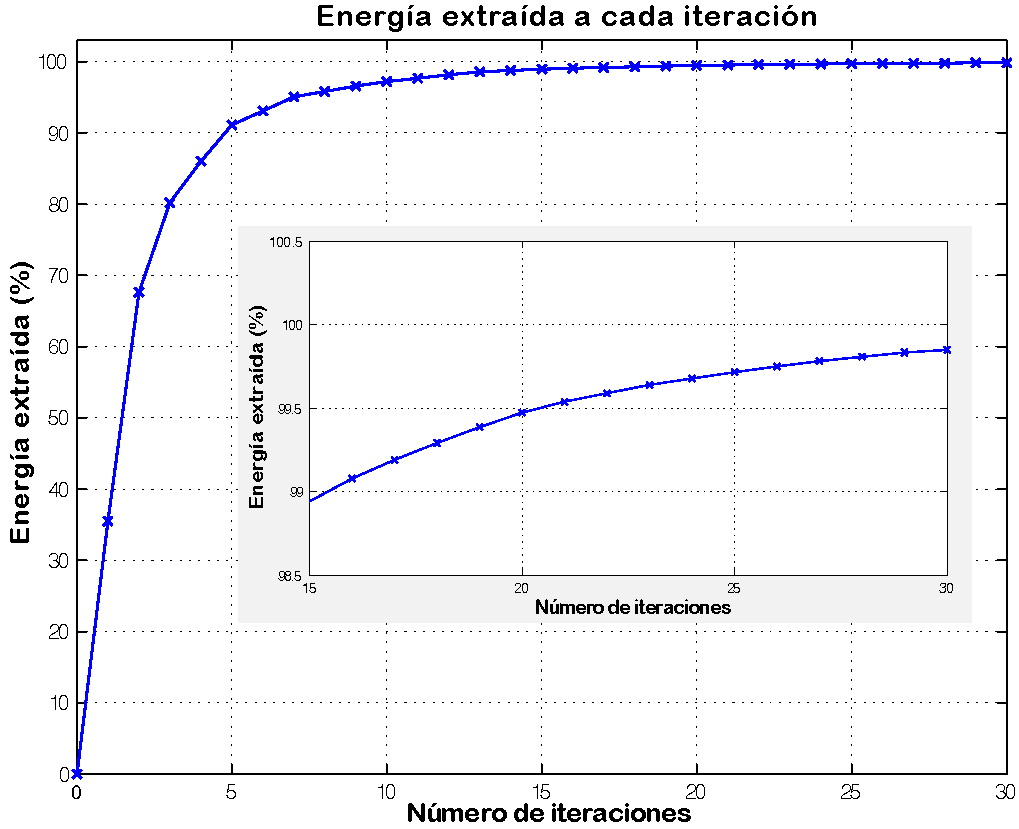
\includegraphics[width=3.5in]
{perfil_energia_extraida.pdf}
\end{center}
\par
\caption{Porcentaje de energía recobrada/extraída tras cada iteración realizada en Matching Pursuit. Se observa en el acercamiento a la gráfica que tras $M=30$ iteraciones realmente no se retiene el total de la energía.}
\label{porcentEnergia}
\end{figure}
%=======================================

Dado este comportamiento, en este trabajo se ha decidido representar mediante MP un 99\% de la energía de la señal, preservando el 1\% restante en la señal residual $R_{M}(t)$. Este residuo tiene correlación mucho más baja con respecto a las ondas de Gabor que el evento cardiaco inicial, que al igual que los silencios aún son perceptibles al oído humano debido al comportamiento logarítmico de este órgano natural receptor \cite[]{Smith1999}. 
 
 En la Figura \ref{eventoRecons} se ha realizado la reconstrucción de un evento cardíaco s1 con 10 iteraciones, cantidad necesaria para representar en un 99 \% su energía. Se muestra la forma de onda temporal de la señal original, el residual y la señal reconstruida, así como la representación en el plano tiempo-frecuencia en cajas de Heisenberg de los átomos necesarios para la descomposición. 
%================================
\begin{figure}[ht]
\begin{center}
\includegraphics[width = 6.8 in]
{eventoRecons.eps}
\end{center}
\par
\caption{Forma de onda temporal y gráfica en el plano tiempo-frecuencia en la reconstrucción de un evento cardiaco s1.}
\label{eventoRecons}
\end{figure}
%=======================================

La señal residual se modelará con técnicas de predicción lineal (LPC), presentadas en el siguiente capítulo. Esta señal se considera como la parte \emph{estocástica} del códec.

} }%
%BeginExpansion
\chapter{Modelado de la parte determinística \\ mediante Matching Pursuit}\label{capit:cap3}
\vspace{-2.0325ex}%
\noindent
\rule{\textwidth}{0.5pt}
\vspace{-5.5ex}% 
\newcommand{\pushline}{\Indp}% Indent puede ir o no :p


Este capítulo presenta una breve descripción del algoritmo iterativo \emph{Matching Pursuit} (MP), que descompone una señal en una combinación lineal de formas de onda elementales pertenecientes a un diccionario redundante de funciones. La compresión se realiza debido a que esta técnica es del tipo \emph{representación dispersa} de señales, es decir, mediante un número reducido de ondas se representan eventos cardiacos extrayendo una gran cantidad de su energía. De igual manera MP es conocido como un método de \emph{representación atómica}, dado que los bloques o diccionarios redundantes de funciones que se les conoce también como \emph{átomos}.

Se ha seleccionado un diccionario multi-bloques para la descomposición cuyos elementos son conocidos como \emph{átomos de Gabor} dada su alta correlación con los eventos cardiacos. 

\section{Representación dispersa de señales}

Una herramienta que ha demostrado ser eficiente en el análisis y representación de señales es la representación dispersa \cite[]{Gribonval2003,Gribonval2007,Elad2010,Mallat1993}. Varios de los procedimientos efectuados en el tratamiento de  señales de audio e imágenes como la transformación, compresión, \emph{de-noising}, separación de fuentes y otros métodos de codificación se han efectuado con eficiencia mediante esta técnica. A continuación se da una breve definición sobre la representación dispersa\footnote{Es conocida en Inglés como \emph{sparse representation.}} de señales.

El objetivo de la representación dispersa es encontrar una representación eficiente de un vector o señal $\mathbf{v} \in \mathcal{H}$, donde $\mathcal{H}=\mathbb{R}^{N}$

Una solución sencilla consistiría en tomar una base ortonormal $\Phi =\{ \phi_{1}, ..., \phi_{N}\}$ para $\mathcal{H}$ y usar los coeficientes de Fourier $\{\langle \mathbf{v},\phi_{k}\rangle\}_{k=1}^{N}$ para representar a $\mathbf{v}$. Esta respuesta es simple y funciona adecuadamente en muchos casos, sin embargo, también puede considerarse un tipo de expansión más general donde la base ortonormal es reemplazada por un diccionario adaptado formado desde $\mathcal{H}$. 

Un \textbf{diccionario} en $\mathcal{H} = \mathbb{R}^{N}$ es una familia de $K  > N$ vectores columna unitarios $\{\mathbf{g_{k}}\}$ que expande o genera a $\mathcal{H}$. En notación matricial se puede expresar como $\mathcal{\mathbf{D}} =[\mathbf{g_{1}},...,\mathbf{g_{K}}]$. 

Se entiende como una representación de $\mathbf{v}$ en $\mathcal{\mathbf{D}}$ un vector columna $\mathbf{\alpha} = (\alpha_{k}) \in \mathbb{R}^{K}$ tal que $\mathbf{v}=\mathcal{\mathbf{D}}\mathbf{\alpha}$. Es importante verificar que $K > N$, esto es, los vectores en $\mathcal{D}$ no son lo suficientemente independientes linealmente y la representación de $\mathbf{v}$ no es única. Se espera que para todas las representaciones posibles de $\mathbf{v}$ exista una \emph{muy reducida}, esto es, la representación con el menor número de coeficientes diferentes de cero. Este procedimiento es representado de manera sencilla en la Figura \ref{sparse_diagram}, donde se verifica que los pocos elementos distintos de cero del diccionario conforman la representación dispersa ideal de $\mathbf{v}$.
%================================
\begin{figure}[ht]
\begin{center}
\includegraphics[width=5.3in]
{sparse_diagram.pdf}
\end{center}
\par
\caption{Representación gráfica de una representación dispersa para una señal $\mathbf{v}$ desde un diccionario $\mathcal{\mathbf{D}}$.}
\label{sparse_diagram}
\end{figure}
%=======================================

Un compromiso que representa un problema en este proceso es el de encontrar todas las representaciones de $\mathbf{v}$ para encontrar las representaciones dispersas (procedimiento que lleva un largo tiempo) y entonces determinar si existe un conjunto único de representaciones dispersas. Varios tipos de diccionarios así como diversos procedimientos y modificaciones a los mismos se han analizado en la literatura para resolver esta encomienda en el menor tiempo posible \cite[]{Gribonval2007,Gribonval2003,Elad2010,RuizReyes2010}.

\section{Diccionarios tiempo-frecuencia}
Es a través de la transformada de Fourier como se describe una señal en términos de su contenido en frecuencia, lo cual se trata de una combinación de formas de onda ortogonales. Esta herramienta es la de uso más común en el análisis de señales en el dominio frecuencial debido a la facilidad que presentan las funciones senoidales siendo su base. 

Mediante una transformación por Fourier se lleva a cabo una proyección de una señal $x(t)$ sobre funciones base exponenciales complejas de frecuencia $\omega = 2\pi f$ :
%-----------------------
\begin{equation}\label{transFourier}
	X(\omega) = \int_{-\infty}^{\infty}x(t) e^{-i\omega t} dt,
\end{equation}
%-----------------------
donde $i=\sqrt{-1}$ y $X(\omega)$ es la \emph{transformada de Fourier} de la señal $x(t)$.

Sin embargo, no todas las señales son idealmente representadas por esta transformación, por ejemplo aquellas que presentan transitorios (cambios abruptos en frecuencia para instantes cortos de tiempo), cuyas irregularidades  requieren un análisis en tramos más consistentes. De esta manera surge la Transformada de Fourier de Tiempo Corto (STFT), la cual consiste en simplemente aplicar la transformada de Fourier a estructuras locales (segmentos con traslape) de la señal. 

En la STFT se incluye el uso de una \emph{ventana deslizante} $w(\tau - t)$ cuya localización es desplazada en el eje temporal, con lo que se proveerá un análisis en el plano tiempo frecuencia dado por la expresión \ref{STFT}:
%-----------------------
\begin{equation}\label{STFT}
	S(\omega,t) = \int_{-\infty}^{\infty}x(t)w(\tau-t) e^{-j\omega t} dt.
\end{equation}
%-----------------------
De aquí se deduce que el empleo de ondas bien concentradas\footnote{Que se conozcan completamente tanto en tiempo como frecuencia (finitas en ambos planos).} en el plano tiempo-frecuencia otorgarán una representación más adecuada en caso que la señal presente transitorios. El desarrollo de un modelo para el análisis o descomposición de señales se verá favorecido mediante la selección de los átomos óptimos, esto es que coincidan con las características básicas de la señal tanto en tiempo como en frecuencia \cite[]{Mallat1999}.

\subsection{Diccionario y átomos de Gabor}
El seleccionar un diccionario adecuado es una tarea fundamental en la descomposición y representación escasa de una señal. En la literatura se han propuesto diversos paquetes de ondas tiempo-frecuencia tales como ondeletas (\emph{wavelets}), paquetes de cosenos, transformadas de coseno discreto modificada y diccionarios de Gabor \cite[]{Wolfe2001}, etc. 

Estos bloques de ondas elementales  han sido probados en la reconstrucción de fonocardiogramas \cite[]{Nieblas2014}, obteniendo que los diccionarios de Gabor son los más adecuados para este propósito.

Los átomos de Gabor son ondas cosenoidales que se obtienen por la dilatación, traslación y modulación de una ventana madre $w(t)$, la cual generalmente toma valores reales y positivos además de tener una norma unitaria. La ecuación \eqref{gaborAtom} define esta forma de onda:
%-----------------------
\begin{equation}\label{gaborAtom}
	g_{\gamma}(t) = \frac{1}{\sqrt{s}}w\left(\frac{t-u}{s}\right) e^{i2\pi\xi(t-u)},
\end{equation}
%-----------------------
donde $w$ es una ventana gaussiana deslizante: $w(t)=\sqrt[4]{2}e^{-\pi t^{2}}$, la longitud de esta envolvente es controlada mediante la variable $s$, mientras que $u$ es un desplazamiento para especificar la localización temporal del átomo y $\xi$ es la frecuencia de modulación de la sinusoide. 
%================================
\begin{figure}[ht]
\begin{center}
\includegraphics[width=4.7in]
{atomo_gabor.eps}
\end{center}
\par
\caption{Forma de onda de un átomo de Gabor.}
\label{gaborWaveform}
\end{figure}
%=======================================

Se define entonces como diccionario o bloque de Gabor al conjunto constituido por las ondas previamente descritas: $\Gamma=\{\gamma_{m}\}_{m=1}^{K}$, donde cada uno de sus elementos se definen como $\gamma_{m}=(s_{m},u_{m},\xi_{m})$ . La Figura \ref{gaborWaveform} muestra la forma de onda de un átomo de Gabor. 

\subsection{Descomposiciones atómicas}
Las bases de ondeletas fueron las predecesoras a las bases de Fourier en la reconstrucción de señales. Pocos coeficientes son necesarios para representar las estructuras correspondientes a los transitorios locales de la señal mediante ondeletas \cite[]{Mallat1999}, constituyendo mediante este método un esquema de compresión.

La historia de la reconstrucción por ondeletas comienza con \cite{Haar1911}, quien propuso una función constante cuyas traslaciones y dilataciones constituyen una base ortonormal para la representación de señales. Esta ondeleta lleva su mismo nombre.

Posteriormente \cite{Gabor1946} propuso la descomposición de una señal sobre diccionarios de formas de onda elementales llamados átomos, los cuales tienen un esparcimiento mínimo en el plano tiempo-frecuencia. En efecto, a este método se le denomina descomposición atómica de señales. 

Para la reconstrucción de la señal se lleva a cabo la suma de los átomos tiempo-frecuencia seleccionados del diccionario. Es fundamental el hecho de entender que los diccionarios son bloques de formas de onda atómicos los cuales presenten elementos de características tiempo-frecuencia adaptados a las propiedades de la señal; la mejor representación de la señal es un problema complejo, dado que existen un sinfín de descomposiciones posibles \cite[]{Gribonval2007}. 

Sea una señal continua $x(t)$, cuya representación atómica en un conjunto de $K$ funciones $g_{m}(t)$ tiene la siguiente estructura:
%-----------------------
\begin{equation}\label{atomicDecomp}
	x(t) = \sum_{i=1}^{K}\alpha_{i}g_{i}(t),
\end{equation}
%-----------------------

donde los coeficientes $\alpha_{i}$ denotan la ponderación asociada a cada función átomo $g_{i}(t)$. También deberá asimilarse que la señal $x(t)$ es finita, para que su energía sea adecuadamente representada tanto en tiempo como en frecuencia (esta representación también puede realizarse con una señal discreta $x(n)$ finita de $N$ elementos). 

La selección de funciones elementales o átomos que mejor aproximan a $x(t)$ así como el cálculo de los coeficientes $\alpha_{i}$ puede realizarse mediante diversos métodos \cite[]{Nieblas2014}, en este caso se ha seleccionado el algoritmo iterativo \emph{Matching Pursuit} \cite[]{Mallat1993}.

\subsection{Principio de incertidumbre de Heisenberg}

Es importante en una descomposición atómica el conocer la concentración de energía de las ondas tiempo-frecuencia empleadas, lo cual garantizará una buena reconstrucción de la señal tratada \cite[]{Mallat1999}. En este caso, los átomos de Gabor son construidos por la traslación en tiempo y frecuencia de una ventana $g$:
%-----------------------
\begin{equation}\label{gaborAtom2}
	g_{u,\xi}(t) = g(t-u)e^{i\xi t},
\end{equation}
%-----------------------
donde $u$ y $\xi$ son las traslaciones o desplazamientos en tiempo y frecuencia correspondientemente.

La energía de $g_{u,\xi}$ se concentra en la vecindad de $u$ sobre un intervalo de tiempo de $\sigma_{t}$. La transformada de Fourier $\widehat{G}$ se traslada mendiante $\xi$ por medio de:
%-----------------------
\begin{equation}\label{gaborAtomTF}
	g_{u,\xi}(\omega) = g(\omega-\xi)e^{-iu(\omega-\xi)}.
\end{equation}
%-----------------------
La energía de $\widehat{g}_{u,\xi}$ se localiza sobre la frecuencia $\xi$ en un intervalo de tamaño $\sigma_{\omega}$. Para el plano tiempo-frecuencia $(t,\omega)$ la energía del átomo ${g}_{u,\xi}$ se representa simbólicamente por un \emph{rectángulo de Heisenberg}, el cual está centrado en $(u,\xi)$ y tiene un largo de duración de tiempo $\sigma_{t}$ y un ancho en frecuencia $\sigma_{\omega}$. El principio de incertidumbre de Heiseberg satisface la desigualdad siguiente:
%-----------------------
\begin{equation}\label{Heis}
	\sigma_{t} \sigma_{\omega} \geq \frac{1}{2}.
\end{equation}
%-----------------------
El área del rectángulo de Heisenberg $\sigma_{t}\sigma_{\omega}$ es mínima para una $g$ tipo gaussiana, en cuyo caso hemos visto que los átomos $g_{u,\xi}$ son llamados funciones de Gabor. La Figura \ref{HeisBoxes} otorga una descripción gráfica en cajas de Heisenberg de dos átomos tiempo-frecuencia, cuya estructura gaussiana favorece el soporte en ambos planos.
%================================
\begin{figure}[ht]
\begin{center}
\includegraphics[width=4.7 in]
{gabor_boxes.pdf}
\end{center}
\par
\caption{Representación de dos átomos tiempo-frecuencia en cajas de Heisenberg.}
\label{HeisBoxes}
\end{figure}
%=======================================

\section{Descomposición de fonocardiogramas mediante Matching Pursuit (MP)}
 Tras con anterioridad haber descrito la importancia de las descomposiciones atómicas y la representación escasa de señales por medio de diccionarios tiempo-frecuencia (en específico los definidos por Gabor) es conveniente mencionar un algoritmo que conjunta estas técnicas como lo es Matching Pursuit \cite[]{Mallat1993}. 
 
 Se ha presentado también MP en la literatura como un auxiliar muy completo en el análisis de fonocardiogramas, debido a que la mayor cantidad de la energía de éstos puede concentrarse por medio de este método en una representación de un número iterativo deseado de formas de onda elementales \cite[]{Zhang1998a,Zhang1998b,wang04,Sava1998}. Esto es, la cantidad de iteraciones deseada es proporcional al número de átomos de la representación y cuan mayor sea se preservará en efecto mayor energía en la reconstrucción.
 
Matching Pursuit es un algoritmo codicioso (\emph{greedy}) debido a que en cada iteración sigue extrayendo energía a la señal analizada, resolviendo el problema de la mejor representación analizado al inicio de este capítulo mediante la realización del máximo absoluto del producto interno (también considerado como \emph{correlación} en este caso). Esta operación garantiza el encontrar los átomos que mejor coincidan (\emph{best-match}) con la estructura local de la señal en la iteración correspondiente. 

La combinación lineal de formas de onda elementales, representación escasa o descomposición atómica de una señal $x(t)$ mediante MP está dada por la expresión \eqref{MatchingPursuit}:
%-----------------------
\begin{equation}\label{MatchingPursuit}
	x(t) = \sum_{m=1}^{M} \alpha_{m} \cdot g_{\gamma_{m}}(t) + R_{M}(t),
\end{equation}
%-----------------------
donde $M$ es el número de iteraciones ó átomos deseado en la descomposición, $g_{\gamma_{m}(t)}$ es el átomo $m$-ésimo óptimo del bloque o diccionario (esto es, $\gamma \in \Gamma$), $\alpha_{m}$ el factor de ponderación y $R_{M}(t)$ un término residual surgido de la diferencia entre la señal y el átomo ponderado después de la m-ésima iteración. 

Por medio del Algoritmo \ref{MP} se observan los procedimientos correspondientes a la obtención de dichos términos, donde la relación señal a ruido (Signal to Noise Ratio, SNR) es obtenida como el cociente de la energía de la señal reconstruida por la suma de los átomos ponderados entre la energía de la señal residual.

% ++++++++++++++++++++++++++++++++++++
\begin{algorithm}
\begin{algorithmic}
\REQUIRE $x(t)$, $\mathcal{D}= \{ g_{\gamma}(t), \gamma \in \Gamma \}$
\ENSURE $\alpha_{m}, g_{\gamma_{m}}(t)$
\STATE {$R=x(t)$}
\STATE {$\alpha_{m} = 0$}
\REPEAT 
	\STATE{$g_{\gamma_{m}} = \arg\max_{\gamma \in \Gamma} \lvert \langle R,g_{\gamma} \rangle \rvert$}
	 \STATE{$\alpha_{m} = \langle R,g_{\gamma} \rangle$}
	 \STATE{$R= R-\alpha_{m}\cdot g_{\gamma_{m}}$}
\UNTIL {se alcance la cantidad de iteraciones o SNR deseadas.}
\end{algorithmic}
\caption {Matching Pursuit}
\label{MP}
\end{algorithm}
%++++++++++++++++++++++++++++++++++++

Observando la forma de onda de los átomos de Gabor puede deducirse su alta correlación con los eventos cardíacos, por lo cual solamente estas partes de la señal son adecuadamente modeladas y reconstruidas mediante Matching Pursuit y diccionarios de este tipo logrando una compresión. 

La \emph{segmentación} es el primer paso para el análisis del fonocardiograma, de esta manera se extraerán solamente los sonidos cardiacos principales y patologías para realizar su descomposición. Este proceso puede realizarse de manera manual o automática por medio de algún algoritmo \cite[]{Nieblas2013}.

Durante la segmentación se detectan los tiempos de inicio \emph{(on-set)} y final \emph{(off-set)} de algún sonido normal o patología cardiaca. Estos instantes de tiempo ayudan a diferenciar las partes del fonocardiograma que son silencio y las que se consideran evento.

\subsection{Criterios en la descomposción de fonocardiogramas por MP}

A pesar de tener una reconstrucción aceptable en las señales de fonocardiograma tras representarlas en los átomos seleccionados desde Matching Pursuit el 100\% de la energía realmente nunca es alcanzado, se tiene un comportamiento asintótico entre ésta variable y el número de iteraciones. 

Esto se observa con detenimiento en la Figura \ref{porcentEnergia}, para lo cual se ha hecho un acercamiento en la parte donde parece haberse restablecido el total de la energía (de las 21 a las 30 iteraciones). 

%================================
\begin{figure}[h!]
\begin{center}
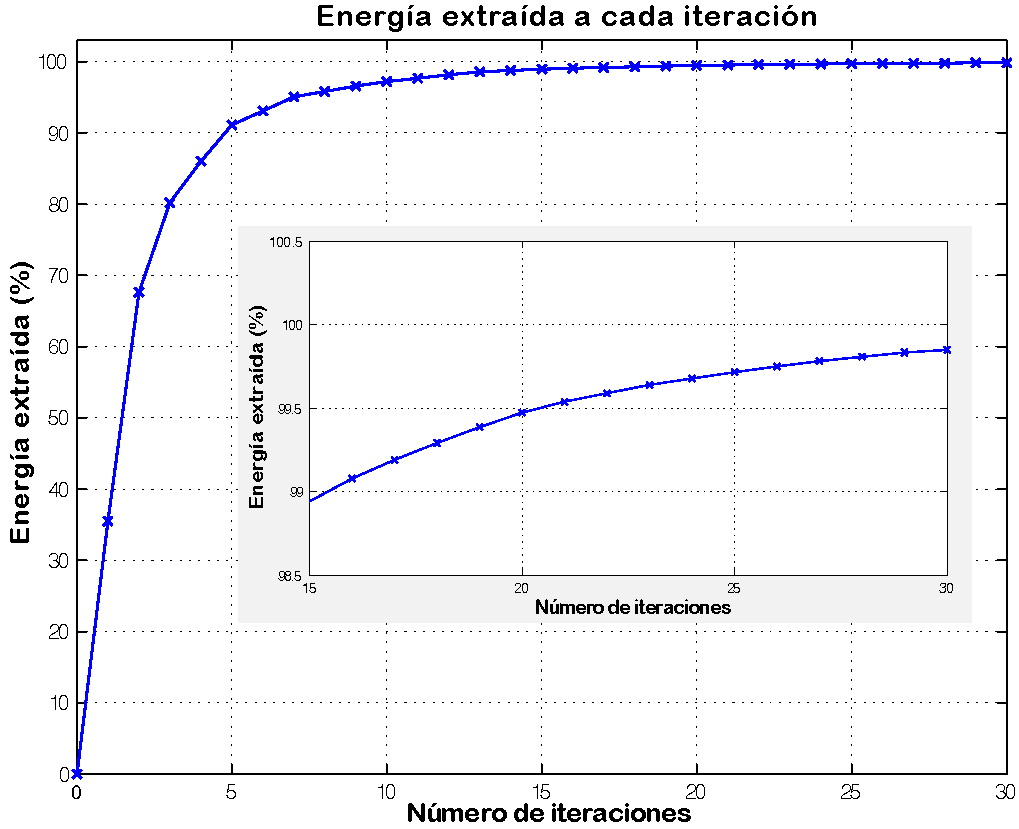
\includegraphics[width=3.5in]
{perfil_energia_extraida.pdf}
\end{center}
\par
\caption{Porcentaje de energía recobrada/extraída tras cada iteración realizada en Matching Pursuit. Se observa en el acercamiento a la gráfica que tras $M=30$ iteraciones realmente no se retiene el total de la energía.}
\label{porcentEnergia}
\end{figure}
%=======================================

Dado este comportamiento, en este trabajo se ha decidido representar mediante MP un 99\% de la energía de la señal, preservando el 1\% restante en la señal residual $R_{M}(t)$. Este residuo tiene correlación mucho más baja con respecto a las ondas de Gabor que el evento cardiaco inicial, que al igual que los silencios aún son perceptibles al oído humano debido al comportamiento logarítmico de este órgano natural receptor \cite[]{Smith1999}. 
 
 En la Figura \ref{eventoRecons} se ha realizado la reconstrucción de un evento cardíaco s1 con 10 iteraciones, cantidad necesaria para representar en un 99 \% su energía. Se muestra la forma de onda temporal de la señal original, el residual y la señal reconstruida, así como la representación en el plano tiempo-frecuencia en cajas de Heisenberg de los átomos necesarios para la descomposición. 
%================================
\begin{figure}[ht]
\begin{center}
\includegraphics[width = 6.8 in]
{eventoRecons.eps}
\end{center}
\par
\caption{Forma de onda temporal y gráfica en el plano tiempo-frecuencia en la reconstrucción de un evento cardiaco s1.}
\label{eventoRecons}
\end{figure}
%=======================================

La señal residual se modelará con técnicas de predicción lineal (LPC), presentadas en el siguiente capítulo. Esta señal se considera como la parte \emph{estocástica} del códec.


%EndExpansion
\newpage }

{\normalsize
%TCIMACRO{\QSubDoc{Include Capitulo04}{
\chapter{Modelado de la parte estocástica \\ mediante Codificación Predictiva Lineal}\label{capit:cap4}
\vspace{-2.0325ex}%
\noindent
\rule{\textwidth}{0.5pt}
\vspace{-5.5ex}% 
\newcommand{\pushline}{\Indp}% Indent puede ir o no :p

Las señales tratadas en tiempo discreto pueden ser de naturaleza determinística o aleatoria, esto dependerá del tipo de expresiones matemáticas con las que puedan ser caracterizados \cite[]{Hayes96}. 

Los procesos aleatorios discretos en tiempo resultan más complicados de modelar matemáticamente, por ello deben emplearse herramientas de tipo estadístico, por ejemplo la \textbf{correlación}, que es una caracterización de segundo orden estadístico que provee información acerca de cuánto dependen linealmente dos señales. Esta propiedad puede ser aprovechada para diseñar sistemas de predicción de señal.

En el presente capítulo se describirá de manera resumida la técnica de codificación predictiva lineal LPC por sus siglas en Inglés, la cual caracteriza a una señal aleatoria discreta. Es una técnica de compresión y representación de secuencias discretas que en este caso se empleará como modelo de una fuente de ruido (\emph{noise-like}) del codificador de audio a diseñar. Particularmente LPC ha tenido éxito en el caso de la codificación de voz. 

Desde su introducción por \cite{Makhoul1973}, los modelos de predicción lineal han tenido éxito en la codificación de audio debido a su baja complejidad, buena eficiencia y escaso costo computacional. Basándose en técnicas de regresión por mínimos cuadrados se obtiene la envolvente espectral de una señal, la cual proporciona la información suficiente para ser percibida de manera auditiva \cite[]{Makhoul1975}.

Las ecuaciones en diferencias y los filtros digitales son elementos con los que se tratan a las señales en tiempo discreto, en especial de manera estadística por tratarse principalmente de conjuntos de valores aleatorios \cite[]{Hayes96}, por consiguiente se definirán en el presente capítulo. De igual forma es necesario introducir a los modelos autorregresivos (AR) como técnicas de recursividad para la caracterización de algunos de estos procesos. LPC, en efecto, es un modelado autorregresivo. 

En esta sección describen los principales parámetros que emplea LPC al abordar el problema de la predicción lineal tal y como es planteado por \cite{Vaidyanathan2008}.  De igual manera, en este capítulo se ahondará el problema de encontrar los coeficientes que conforman el predictor lineal desde la perspectiva de \cite{Rabiner1978,Rabiner1993}, quien mediante el método de la autocorrelación otorga una respuesta favorable y sencilla que al problema que \cite{Makhoul1975} había introducido de manera determinística.

Por último se extrapolará la idea de predicción lineal desde el dominio temporal hacia el frecuencial \cite[]{Makhoul1975c,Makhoul1973}, donde la autocorrelación actúa como vínculo para lograr una coincidencia en la representación para ambos dominios.

Es necesario resaltar la importancia de LPC como técnica de compresión, tal y como lo manifiesta \cite{Gersho1992}, ya que se lograrán representar segmentos de señal con grandes cantidades de muestras con un escaso número de coeficientes de una representación puramente lineal.

% ----------------------------------------------------------------------------
\section{Filtros digitales y transformada z}
\subsection{Transformada z}
No todas las señales pueden ser descritas por la transformada de Fourier de tiempo discreto (DTFT) para su representación en el dominio frecuencial, por ello se emplea la \emph{transformada z} como generalización para incluir a estas secuencias y representar su caracterización espectral.

La transformada $z$ de una señal en tiempo discreto se define como:
\begin{equation} \label{transf_z}
		S(z)= \sum_{n=-\infty}^{\infty}s(n)z^{-n},
\end{equation}
donde $z=re^{j\omega}$ y teniendo el caso de que cuando $r=1$:
\begin{equation}\label{DTFT}
S(e^{j\omega})=S(z)|_{z=e^{j\omega}} = \sum_{n=-\infty}^{\infty} s(n)e^{-jn\omega},
\end{equation}
siendo entonces lo definido en la ecuación \eqref{DTFT} la misma transformada de Fourier en tiempo discreto (DTFT) de s(n).

Se puede también definir como \emph{función del sistema} a la transformada $z$ de la respuesta al impulso $h(n)$ de un sistema. Esta función servirá para conocer la salida de un sistema a una entrada específica y será de utilidad en las siguientes definiciones:  
\begin{equation}\label{H}
H(z) = \sum_{n=-\infty}^{\infty} h(n)z^{-n}.
\end{equation}
%===================================================
\subsection{Filtros digitales}
Un filtro digital es definido como un sistema lineal e invariante en tiempo (LTI) que modifica bajo circunstancias controladas a una señal discreta tanto en frecuencia como en tiempo \cite[]{Hayes96}. La función  que define a un filtro digital consiste en una ecuación en diferencias, en este caso y por simplicidad de constantes lineales (LCCDE):
\begin{equation}\label{LCCDE}
y(n) +\sum_{k=1}^p a(k)y(n-k)=\sum_{k=0}^q b(k)s(n-k),
\end{equation}
donde $s(n)$ es la entrada y $y(n)$ la salida correspondiente del filtro digital, los enteros $p$ y $q$ determinan su orden mientras que $a(1), a(2) ,..., a(p)$ y $b(0), b(1), ..., b(q)$ lo definen o caracterizan \footnote{Más adelante se analizarán las características de acuerdo a la  magnitud de  estos coeficientes.}.

La salida del sistema $y(n)$ dada por el modelo matemático surge al reescribir la expresión \eqref{LCCDE}:
\begin{equation}\label{LCCDE2}
y(n) =\sum_{k=0}^q b(k)s(n-k) -\sum_{k=1}^p a(k)y(n-k).
\end{equation}
 En efecto, $y(n)$ es una combinación lineal de los valores anteriores $y(n-k)$. De acuerdo a la existencia o no de los coeficientes $a's$ y $b's$ se definen los filtros de respuesta al impulso finita o infinita (FIR o IIR) a continuación.
%9099090909090909090909099090909090909090909090909090909090909090

\subsubsection{Filtros de respuesta al impulso finita (FIR LCCDE)}
De la ecuación \eqref{LCCDE2} en el caso de que $p=0$ la salida $y(n)$ del sistema depende solamente de los valores de entradas anteriores $x(n-k)$ teniendo un \emph{Filtro de Respuesta al Impulso Finita}. 

La función del sistema si se conoce la respuesta al impulso $h(n)$ se define por el siguiente polinomio en $z^{-1}$:
\begin{equation}\label{FIR}
H(z) = \sum_{k=0}^q b(k) z^{-k} = b(0) \prod_{k=1}^q (1-z_kz^{-1}).
\end{equation}
El polinomio determinado por \eqref{FIR} genera raíces $z_{k}$ denominadas ``ceros''. Debido a esta estructura el filtro FIR se define como \emph{todo ceros}.

La figura \ref{FIR_diag} muestra  un diagrama a bloques del filtro FIR, consistente en una serie de retardos $z^{-1}$ conectados en serie y sumados a la salida. Es evidente que el número de bloques deseado es el mismo que indica el orden del sistema.
\begin{figure} [h!]\label{FIR_diag}
  \centering
  \includegraphics[width=8cm]{fir_diag.pdf}
  \caption{Diagrama a bloques de un filtro FIR.}
  \label{FIR_diag}
\end{figure}
%---------------------------------------------------909090909090
\subsubsection{Filtros de respuesta al impulso finita (IIR LCCDE)}
Cuando en la expresión \eqref{LCCDE2} se tiene que $p \ne 0$ la relación entrada-salida o función del sistema está dada por una operación fraccionaria, las raíces de los polinomios del denominador y numerador producen los ceros y polos del sistema respectivamente, los cuales son capaces de dar características sobre la estabilidad del sistema lineal. 

La ecuación \eqref{IIR} denota la función de sistema de un filtro IIR:
\begin{equation}\label{IIR}
H(z) =\frac{\displaystyle \sum^{q}_{k=0} b(k)z^{-k}}{\displaystyle 1+\sum_{k=1}^{p} a(k)z^{-k}} = b(0) \frac{\displaystyle \prod_{k=1}^{q} (1-z_k z^{-1})}{\displaystyle \prod_{k=1} ^p (1-p_k z^{-1})},
\end{equation}
donde las raíces del denominador $p_{k}$ son conocidas como los \emph{polos} del filtro.

Si el orden del polinomio del numerador es igual a cero entonces:
\begin{equation}\label{all_pole}
H(z) =\frac{b(0)}{1+\displaystyle \sum_{k=1} ^p a(k)z^{-k}} =  \frac{b(0)}{\displaystyle \prod_{k=1} ^p (1-p_k z^{-1})}
\end{equation}
y se le conoce como un filtro \emph{todo polos} al no contener ceros.

Teniendo que $a(k), b(k) \in \mathbb{R}$ es posible que $H(z)=H^*(z^*)$, esto es, si $H(z)$ tiene un polo en $z=a$ también tendrá un cero en $z=a^*$. 

Se observa en la figura \ref{iir_diag} la estructura de un filtro IIR, observando que se requieren las muestras de los instantes anteriores de tiempo tanto de la entrada $x(n)$ como de la salida $y(n)$ del filtro. 
\begin{figure} [ht]
  \centering
  \includegraphics[width=10cm]{iir_diag.pdf}
  \caption{Diagrama a bloques de un filtro IIR.}
  \label{iir_diag}
\end{figure}

%*****************************************************
\section{Modelos autorregresivos}
Un proceso estacionario en sentido amplio $w(n)$ (WSS) \footnote{Proceso estacionario en sentido amplio: señal aleatoria o proceso estocástico que en sus valores no guarda correlación estadística en dos instantes de tiempo diferentes.} \cite[]{Papoulis1984} se dice que es autorregresivo $AR$ si puede ser generado empleando una ecuación en diferencias recursiva como la siguiente:
\begin{equation}\label{ar}
w(n) = -\sum_{i=1}^N d_i^* w(n-i)+e(n)
\end{equation}

Donde $e(n)$ es también un proceso WSS con media cero.

Suponiendo que el siguiente polinomio es \emph{todos ceros}:
\begin{equation}\label{ar_coef}
D(z) = 1+\sum_{i=1}^N d_i^* z^{-i}
\end{equation}
se tiene ahora que $w(n)$ es la salida de un filtro IIR \emph{todo polos} definido por $1/D(z)$ en respuesta a una entrada $e(n)$. Si los coeficientes $d_i \ne 0$ el proceso es $AR(n)$ ($AR$ de orden $n$). El proceso $e(n)$ es WSS, tiene media cero y es de ruido blanco.

En la Figura \ref{AR_diag} se muestra el modelo de un proceso AR como salida de un filtro de respuesta al impulso infinita cuya entrada es un proceso de ruido blanco.

\begin{figure} [h!]\label{AR_diag1}
  \centering
  \includegraphics[width=6cm]{AR_diag1.pdf}
  \caption{Modelo AR como salida de un filtro IIR en respuesta a una entrada de un proceso blanco.}
  \label{AR_diag}
\end{figure}

Si se supone que para un proceso WSS $s(n)$ se ha encontrado el polinomio predictor de coeficientes $A_N(z)$ de $n$-ésimo orden, y además como se mencionó anteriormente, se puede representar como la salida de un filtro IIR, se tiene que la entrada a este sistema es el error de predicción $e_{N}(n)$  y en dominio temporal se puede expresar como:
\begin{equation}\label{ar_xn}
s(n) = -\sum_{i=1}^N a_i^* s(n-i)+e_N(n).
\end{equation}
Prácticamente $e_N(n)$ tiende a ser cercanamente blanco si $N$ es razonablemente grande. Si se reemplaza a este proceso por ruido blanco con media cero, $e(n)$, y conociendo el error medio cuadrático $\epsilon_N$ se obtendrá el modelo $AR$ al cual denominaremos $y(n)$ del proceso $s(n)$.

\section{Codificación mediante predicción lineal}

La idea básica de codificación predictiva lineal (LPC) consiste en que una muestra de un proceso aleatorio puede ser representado como una combinación lineal de las muestras anteriores, en la codificación se representan las envolventes en energía y en frecuencia como parámetros del modelo por medio de \emph{coeficientes de predicción} de un filtro digital.

El conjunto de coeficientes predictores es único y puede determinarse minimizando la suma de las diferencias al cuadrado (la cual se denominará como \emph{error cuadrático}) sobre un intervalo finito entre la muestra actual y las predichas linealmente.

Las muestras de una señal aleatoria discreta $s(n)$ pueden ser producidas por una señal de excitación $u(n)$ como se describe en la siguiente ecuación:
\begin{equation}\label{lpc1}
s(n) = \sum_{k=1}^p a_k \cdot s(n-k)+Gu(n),
\end{equation}

donde $a_{k}$ son los coeficientes predictores y $G$ es la ganancia del filtro predictor; $u(n)$ es la señal de excitación a la entrada del filtro. 

La función $H(z)$ que relaciona la entrada y la salida del sistema del filtro es la siguiente:
\begin{equation}\displaystyle
\label{trans_predic}
H(z) = \frac{S(z)}{U(z)}=\frac{G}{\displaystyle 1-\sum_{k=1}^{p} a_{k}z^{-k}},
\end{equation}
esto es un modelo denominado \emph{todo polos} con el cual se representan secuencias de voz de manera natural \cite[]{Rabiner1993,Rabiner1978} y será utilizado en el codificador diseñado en esta tesis para el modelado de la parte estocástica.

Un predictor lineal de $p$-ésimo orden es un sistema de la forma:
\begin{equation}\label{predic_lineal}
\hat{s}(n) = \sum_{k=1}^p\alpha_{k}s(n-k) \Leftrightarrow P(z) = \sum_{k=1}^{p} \alpha_{k}z^{-k}.
\end{equation}

A la diferencia entre las muestras de señal originales y las muestras estimadas por el predictor lineal se le conoce como \emph{error de predicción} $e(n)$, el cual está dador por:
\begin{equation} \label{error}
e(n)= s(n)-\hat{s}(n) = s(n)-\sum_{k=1}^{p} \alpha_{k}s(n-k). 
\end{equation}

El error de predicción es también la salida de un sistema con la siguiente función de transferencia:
\begin{equation}\label{trans_az}
A(z) = \frac{E(z)}{S(z)} = 1-P(z) = 1-\sum_{k=1}^p \alpha_{k}z^{-k},
\end{equation}

si la secuencia original $s(n)$ cumple exactamente con el modelo de predicción se tendrá una reconstrucción original. Esto se traduce a que $\alpha_{k} = a_{k}$, para $1\leq k \leq p $, $e(n)=Gu(n)$ y además $A(z)$ es un filtro inverso para $H(z)$, esto es:
\begin{equation}\label{trans_hz}
H(z) = \frac{1}{A(z)}.
\end{equation}
En la Figura \ref{lpc_diag2} se muestra un diagrama del modelo de predicción lineal LPC, conjuntando las etapas de obtención de $s(n)$ en cascada por medio del sistema todo polos (parte izquierda) y de reconstrucción por medio del filtro $A(z)$ (parte derecha).

\begin{figure} [ht]
  \centering
  \includegraphics[width=5.5in]{lpc_diag2.pdf}
  \caption{Modelo de predicción lineal.}
  \label{lpc_diag2}
\end{figure}

Por otra parte, la Figura \ref{lpc_diag1} muestra la generación de una secuencia $s(n)$ mediante LPC, la creación de la señal del error de predicción $e(n)$ y mediante ésta la reconstrucción ideal de $s(n)$.

\begin{figure} [h!]
  \centering
  \includegraphics[width=7.2cm]{lpc_produc.pdf}
  \caption{Modelado mediante LPC. En la parte a) se produce una secuencia $s(n)$ por el modelo todo polos. La parte b) muestra la generación de $e(n)$ como salida del filtro $A(z)$, cuya inversión en c) reproduce idealmente a $s(n)$ si tiene como entrada al error de predicción $e(n)$.}
  \label{lpc_diag1}
\end{figure}

%====================================================

\subsection{Modelo de predicción lineal}
La naturaleza aleatoria de una secuencia de entrada $s(n)$  de audio ha forzado el calcular los coeficientes de un filtro de predicción en segmentos pequeños de la señal (comúnmente de 10-20 ms para el caso de la voz) \footnote{En nuestro caso, el audio cardiaco posee baja correlación con los bloques de reconstrucción del modelo determinista elegido, por lo tanto el residual se considerará de esta naturaleza y se analizará también en segmentos o tramos de la misma longitud.}.

Las características del error de predicción $e(n)$ son importantes para definir qué clase de secuencia elegir como la entrada $u(n)$.

Según los trabajos realizados por \cite{Rabiner1978}, se tienen dos casos para esta elección :
\begin{itemize}
	\item{Trama de audio vocalizada \emph{(voiced sound)}}: El segmento analizado de audio provee a la salida una señal de $e(n)$ 		con características \textbf{periódicas}, donde se ha encontrado una frecuencia fundamental $f_0$ (llamada también tono o 		\emph{pitch}). Dada esta  periodicidad, se elige a $u(n)$ como un tren de pulsos con periodo $T_0$ (\emph{pitch period})\footnote{En el caso de las 		señales de voz ejemplos de sonidos vocalizados son los producidos al pronunciar fonemas como los de las letras ``a'', ``o'', entre 		otras.}.  
	\item{Trama de audio no vocalizada \emph{(unvoiced sound)}}: Se tiene un segmento de audio que arrojó a la salida una secuencia $e(n)$ 		que \textbf{no presenta periodicidad alguna}, sus características son similares a las de una fuente de ruido blanco gaussiano y se elige a $u(n)$ como una secuencia aleatoria con este comportamiento\footnote{Sonidos como el de la ``s''  presentan este comportamiento.}.
\end{itemize}

Las características anteriores permiten producir a $s(n)$ a través de una señal de excitación $u(n)$  que será la entrada de un filtro inverso predictor  lineal \footnote{Se trata de un filtro con las mismas características que el filtro de predicción FIR lineal directo, sólo que la operación de filtrado se realiza de manera inversa.}. 

En las siguientes secciones se abordará el problema de encontrar los coeficientes de predicción $\alpha_k$ y la ganancia $G$ que acompaña o complementa a $u(n)$.

%=================================================================
\subsection{Predicción hacia adelante y hacia atrás}
Como anteriormente se había considerado, la predicción lineal consiste en representar una muestra $s(n)$ de una secuencia discreta a partir de la combinación lineal de los $p$ valores anteriores $$s(n-1),s(n-2),...,s(n-p).$$
El predictor lineal diseñado a partir de estos valores fue definido en la ecuación \eqref{predic_lineal}. A este procedimiento se le conoce como \emph{predicción hacia adelante (forward prediction)} ya que se está prediciendo a partir de las muestras consecuentes en el tiempo.

En contraste, también es posible predecir \emph{hacia atrás (backward prediction)}, usando las mismas $p$ muestras u observaciones de la señal en una combinación lineal pero ahora para estimar el valor $s(n-p-1)$ en un instante o unidad de tiempo anterior al valor observado. 

Dadas estas condiciones el predictor \emph{hacia atrás} se define como:
\begin{equation}\label{forw_predic}
\hat{s}(n-p-1)= -\sum_{k=1}^p b_{k} \cdot s(n-k).
\end{equation}
Ahora las mismas muestras relativas al instante de tiempo $n-p-1$ son vistas como \emph{valores futuros} y los coeficientes que denotan la predicción hacia atrás se denotan como $b_k$. La Figura \ref{lpc_samples2} denota la simetría existente entre la predicción hacia adelante y hacia atrás, esto es, se emplean las mismas $i$ muestras.

\begin{figure}[ht]
  \centering
  \includegraphics[width=13.1cm]{lpc_samples2.pdf}
  \caption{Simetría entre la predicción hacia adelante y hacia atrás.}
  \label{lpc_samples2}
\end{figure}

%=================================================================
\subsection{Estimación de los coeficientes de predicción}

En el procedimiento de LPC, una tarea muy importante es la de encontrar los coeficientes predictores $\alpha_k$ que minimicen el \emph{error cuadrático medio} $E$, definido como:
\begin{equation}\label{err_cuad}
E=\sum_{n=-\infty}^\infty e(n)^2.
\end{equation}
Para esto existen los métodos basados en la autocorrelación y autocovarianza, se ha elegido el primero de ellos a manera de ilustrar con simplicidad la determinación de los $\alpha_k$'s.

De acuerdo a la expresión \eqref{err_cuad} para calcular $E$ podemos reemplazar a $e(n)$ de acuerdo a como se definió en \eqref{error} y tendremos que:
\begin{equation}\label{err_cuad2}
E = \sum_{n=-\infty}^\infty (s(n)-\hat{s}(n))^2 = \sum_{n=-\infty}^\infty \left[s(n)- \sum_{k=1}^p \alpha_k s(n-k) \right]^2.
\end{equation}

El predictor lineal óptimo es aquel diseñado para el mínimo valor de $E$. De acuerdo a lo mencionado en \cite{Makhoul1975}, la minimización ocurrirá cuando: 
\begin{equation}\label{min_E}
\frac{\partial E}{\partial \alpha_i}=0,
\end{equation}
para $i=1,2,3,...,p$, logrando diseñar un predictor de resolución variable de acuerdo al número de coeficientes.

Realizando la derivación parcial de $E$ con respecto a $\alpha_i$ como lo indica \eqref{min_E} desde \eqref{err_cuad2} se tendrá que:
$$\frac{\partial E}{\partial \alpha_i}=\sum_{n=-\infty}^\infty 2\left[s(n)- \sum_{k=1}^p \alpha_k s(n-k) \right][-s(n-i)]=0,$$
$$\sum_{n=-\infty}^\infty s(n)s(n-i)-\sum_{n=-\infty}^\infty \sum_{k=1}^p \alpha_k s(n-k)s(n-i)=0$$
$$\sum_{n=-\infty}^\infty s(n)s(n-i)-\sum_{k=1}^p \alpha_k \sum_{n=-\infty}^\infty s(n-k)s(n-i)=0,$$
de donde se puede obtener un sistema de $p$ ecuaciones lineales simultáneas:
\begin{equation}\label{eqs}
\sum_{k=1}^p \alpha_k \sum_{n=-\infty}^\infty s(n-k)s(n-i)=\sum_{n=-\infty}^\infty s(n)s(n-i),
\end{equation}
el cual puede resolverse empleando la autocorrelación, definida como:
\begin{equation}\label{autocorrelacion}
R(k) = \sum_{n=-\infty}^{\infty} s(n)s(n-k) = \sum_{n=-\infty}^{\infty} s(n)s(n+k) ,
\end{equation}
 esta función es simétrica, es decir, se cumple que $R(k)=R(-k)$.

Suponiendo que la señal $s(n)$ ha sido segmentada o \emph{ventaneada}, es decir $s(l)=0$ para $l<1$ ó $l>N$, 
puede realizarse un cambio de variable $n-k$ por $l$ en \eqref{eqs} para compactar en \eqref{autocorrelacion} al término que acopaña a la sumatoria de $a_k$, esto es:
$$\sum_{n=0}^\infty s(n-k)s(n-i) \rightarrow \sum_{l+k=-\infty}^{l+k=\infty} s(l)s(l+k-i) = R(i-k),$$

de la misma forma en \eqref{eqs} se puede denotar una expresión cerrada como la \eqref{autocorrelacion} en el término de la derecha, con lo que se tendrá:
$$\sum_{n=-\infty}^\infty s(n)s(n-i) = R(i).$$
Es importante observar que los límites de la sumatoria se conservan dada la suposición de que los valores de $s(n)$ son cero fuera del intervalo $0\le l \le N-1$, lo cual puede realizarse multiplicando esta secuencia por una ventana de tiempo.

El procedimiento completo de realizar las sustituciones en \eqref{eqs} es el siguiente:
\begin{equation}\label{corrs}
\sum_{k=1}^p \alpha_k \sum_{n=-\infty}^\infty s(n-k)s(n-i)=\sum_{n=-\infty}^\infty s(n)s(n-i) \rightarrow \sum_{k=1}^p \alpha_k R(i-k)=R(i).
\end{equation}

 Si se continúa desarrollando para $i=1, 2, ..., p$ lo definido en \eqref{corrs} se produce el siguiente conjunto de ecuaciones lineales:
\begin{eqnarray*}
\alpha_1R(0)+\alpha_2R(1)+\alpha_3R(2)+...+\alpha_p R(p-1)=R(1) \\
\alpha_1R(1)+\alpha_2R(0)+\alpha_3R(1)+...+\alpha_p R(p-2)=R(2) \\
\alpha_1R(2)+\alpha_2R(1)+\alpha_3R(0)+...+\alpha_p R(p-3)=R(3) \\
\hdots  \\
\alpha_1R(p-1)+\alpha_2R(p-2)+\alpha_3R(p-3)+...+\alpha_p R(0)=R(0).
\end{eqnarray*}
\clearpage
Reescribiendo de manera matricial el conjunto de ecuaciones de \eqref{corrs} se tiene:

\begin{equation}
\left[
\begin{array}{l c c c r}
R(0) 		& R(1) 	& \cdots & R(p-2) & R(p-1) \\
R(1) 		& R(0) 	& \cdots & \cdots & R(p-2) \\
\vdots 	& \vdots 	& \vdots & \vdots & \vdots \\
R(p-2) 	& \cdots 	& \cdots & R(0) & R(1) \\
R(p-1) 	& R(p-2) 	& \cdots & R(1) & R(0) \\
\end{array} \right] 
\left[\begin{array}{c}
\alpha_1 \\
\alpha_2 \\
\vdots \\
\vdots \\
\alpha_p \\
\end{array} \right]=
\left[\begin{array}{c}
R(1) \\
R(2) \\
\vdots \\
\vdots \\
R(p) \\
\end{array} \right],
\label{mat_eqs}
\end{equation}
que en forma compacta corresponde a:
%----------------------------------
\begin{equation}\label{comp_mat_eqs}
\mathbf{R}\mathbf{\alpha}=\mathbf{r}.
\end{equation}
%------------------------------------
El conjunto de soluciones $\alpha_k$ corresponde al vector $\mathbf{\alpha}$ que se obtiene algebraicamente por:
$$\mathbf{\alpha} = \mathbf{R}^{-1} \mathbf{r}.$$
La matriz $\mathbf{R}$ del sistema \eqref{comp_mat_eqs} es de tipo\emph{Toeplitz}\footnote{Matriz cuadrada que se caracteriza por tener los mismos elementos en las diagonales de izquierda a derecha (son constantes).}, simétrica\footnote{Obsérvese su simetría en la igualdad de los valores triangular inferior y superiores, que los elementos en la diagonal principal son los mismos y que es cuadrada en efecto.} y definida positiva \cite[]{Gray2006}. Con ello, el cálculo de la energía de la señal $R(0)$ dará los valores de la diagonal principal en esta matriz. 

El método denominado recursión de Levinson-Durbin es adecuado para resolver este sistema de ecuaciones y se explicará en la siguiente sección.
\subsubsection{Recursión de Levinson-Durbin}
La estructura \eqref{mat_eqs} presenta propiedades para derivar un algoritmo recursivo que permita invertir la matriz $\mathbf{R}$, además de observar en esta misma expresión que el vector $\mathbf{r}$ es una versión sintetizada\footnote{En efecto, $\mathbf{r}$ presenta sólo una vez los valores de $R(1)$ a $R(p)$ mientras que $\mathbf{R}$ repite a éstos y contiene además a $R(0)$.} del contenido existente en $\mathbf{R}$.

El algoritmo de Levinson-Durbin se ha formulado para diseñar un filtro predictor hacia adelante de tamaño $p$ de memoria, comenzando con cero y realizando iteraciones en una cantidad deseada actualizando su tamaño \cite[]{Rabiner1978,Hayes96,Vaidyanathan2008}.  Se trata de un procedimiento que por medio de una \emph{recursión} determina el óptimo predictor de $i$-ésimo orden a partir del $(i-1)$-ésimo predictor (filtro anterior).

Los valores de autocorrelación de $\mathbf{R}$ determinan los coeficientes de reflección $k_i$ y los coeficientes de predicción $\alpha_i$ calculándose de manera consecutiva.

 La función del sistema del error de predicción $A(z)$ definida en \eqref{trans_az} satisface que:
$$A^{(i)}(z)=A^{(i-1)}(z)-k_iz^{(-i)}A^{(i-1)}(z^{(-1)}).$$
Esto es, el $i$-ésimo error de predicción hacia adelante  $e^{(i)}(n)$ es la salida de la $i$-ésima función de sistema del filtro de error de predicción $A^{(i)}(z)$.Todos los ceros de este sistema estrictamente se encuentran dentro del círculo unitario del plano $z$ \cite[]{Makhoul1975}. 

El Algoritmo 2 es el procedimiento de recursión de Levinson-Durbin, donde es importante verificar que el índice superior marcado entre paréntesis denota el orden $p$-ésimo del predictor previamente seleccionado y el índice inferior el $i$-ésimo coeficiente a calcular.
\begin{algorithm}
\begin{algorithmic}
\STATE {$E^{0}=R(0)$;}
\FOR   {$i=1,2,...,p$}
	\STATE { $k_i =\frac{\displaystyle \left(R(i)-\sum_{j=1}^{i-1}\alpha_j^{(i-1)}R(i-j)\right)}{ E^{(i-1)}}$ }
	\STATE {$\alpha_i^{(i)}=k_i$}
	\IF{$i > 1$}
		\FOR   {$j=1,2,...,i-1$}
			\STATE {$\alpha_j^{(i)}=\alpha_j^{(i-1)}-k_i\alpha_{i-j}^{(i-1)}$}
		\ENDFOR
	\ENDIF
	\STATE{$E^{(i)}=(1-k_i^2)E^{(i-1)}$}
\ENDFOR
\STATE{$\alpha_j=\alpha_j^{(p)}$}
\STATE{$j=1,2,..,p$}
\end{algorithmic}
\caption{Recursión de Levinson-Durbin}
\label{levinson}
\end{algorithm}
Los coeficientes de reflección $k_i$, obtenidos a la par que los coeficientes $\alpha_{i}$ de predicción a la salida del algoritmo de Levinson, también son denominados \emph{PARCOR}. Esto se debe a que son obtenidos por medio de correlaciones parciales (del Inglés \emph{partial correlation}). 

Una propiedad muy importante es que para todos los coeficientes reflectores se cumple que $|k_i|\leq 1$, lo cual sirve para garantizar la estabilidad del filtro predictor\footnote{Esta propiedad será importante al cuantificar.}.

 \cite{Itakura1975,Itakura1968} lograron establecer una forma para calcular directamente estos coeficientes mediante una expresión que relaciona los valores de la correlación cruzada con los errores de predicción hacia adelante y hacia atrás, esto es:
\begin{equation}
k_i =\frac{\displaystyle \sum_{m=-\infty}^\infty e^{(i-1)}(m)b^{(i-1)}(m-1)}{\displaystyle\left(\sum_{m=-\infty}^\infty \left(e^{(i-1)}(m)\right)^2 \sum_{m=-\infty}^{\infty}\left(b^{(i-1)}(m-1)\right)^2 \right)},
\end{equation}
Donde $b^{(i)}(m)$ es la salida de error de predicción del filtro hacia atrás. 
%---------------------------=========================================================================
\section{Estimación espectral}
 La interpretación en dominio frecuencial del análisis de predicción lineal por medio de la autocorrelación, provee información necesaria para representar el espectro de potencia de una señal dado por la STFT \cite[]{Rabiner1993}. 

Todo parte del principio fundamental de que la función de autocorrelación $R(n)$ es un proceso inverso al cálculo de magnitud al cuadrado del valor absoluto de la transformada de Fourier $|S(e^{j\omega})|^{2}$ (conocido también como \emph{espectro de potencia de la señal}). 

El espectro de potencia estimado por LPC $\widehat{P}(\omega)$ ó $|\widehat{S}(\omega)|^{2}$, corresponde al cálculo de la magnitud al cuadrado de la transformada de Fourier de la función del sistema $H(z)$ que se expresó en \eqref{trans_predic}:
\begin{equation}\label{pow_estim}
\widehat{P}(\omega)=|\widehat{S}(\omega)|^{2}=|H(e^{j\omega})|^2=\frac{G^2}{|A(e^{j\omega})|^2},
\end{equation}
donde se ha sustituido $z$ por $e^{j\omega}$.

Por otra parte, el espectro de potencia de la señal original $|S(e^{j\omega})|^{2}$ ó $P(\omega)$ es obtenido a partir de la función de sistema del error de predicción. Este espectro se calcula despejando $S(z)$ de \eqref{trans_az}, y de igual manera, sustituyendo $z$ por $e^{j\omega}$ se obtiene:
\begin{equation}\label{pow_espec}
P(\omega) = |S(e^{j\omega})|^{2} =\frac{|E(e^{j\omega})|^2}{|A(e^{j\omega})|^2}.
\end{equation}
Comparando el espectro estimado por LPC calculado en \eqref{pow_estim} y el espectro original definido en \eqref{pow_espec} se ha demostrado que $|E(e^{j\omega})|^2$ es modelado por una señal de espectro plano (ruido blanco, por ejemplo) $G^2$, dado este efecto al filtro $A(z)$ también se le conoce como \emph{blanqueador} ya que produce una señal de este tipo \cite[]{Makhoul1973}.

Los transitorios que determinen la estacionareidad de la señal afectarán el cálculo de $P(\omega)$ y por consiguiente su autocorrelación (que ahora se denotará como $R_{\hat{n}}(i)$). Por lo tanto, la señal variará muy rápidamente en el tiempo y es preciso que sea \emph{ventaneada}: 
$$s_{\hat{n}}(m)=s(n+m) \cdot w(m),$$
donde la señal $w(m)$ es una \emph{ventana} de tiempo que idealmente sería rectangular y cuya función es hacer que se tenga estacionareidad por un gran periodo de tiempo.

En este caso, la transformada de Fourier de tiempo corto \emph{STFT} es la herramienta auxiliar para calcular el espectro de la señal $P(\omega)=|s_{\hat{n}}(e^{j\omega})|^2$ y el espectro estimado, dado por:
$$\left|H(e^{j2\pi f/fs})\right|^2=\left|\frac{G}{1-\displaystyle \sum_{k=1}^p \alpha_k H(e^{-j 2\pi f/fs})}\right|^2$$
siendo $f_s$ la frecuencia de muestreo de $s(n)$.

En la Figura \ref{lpc_aprox} se observa lo realizado por LPC en términos de la aproximación de la envolvente espectral de energía para una señal residual de audio cardiaco. La resolución en esta envolvente radica en incrementar el orden del filtro predictor.
%------------------------------------------------------------
\begin{figure}[ht]
  \centering
  \includegraphics[scale=0.47]{lpc_aprox.eps}
  \caption{Aproximación por codificación predictiva lineal para una señal de audio cardiaco con un orden de filtro $p=30$.}
  \label{lpc_aprox}
\end{figure}
% -------------------------------------------------------------

La predicción del \emph{futuro} mediante procedimientos estadísticos desde luego que no es con certeza, pero es posible determinar una estructura similar a través de la inercia presentada en las observaciones del pasado y el presente, premisa retomada por las técnicas matemáticas de predicción en secuencias discretas que son de tipo aleatorio \cite[]{Gersho1992}.

En el caso de la predicción lineal se tiene una versión especializada de la teoría de estimación por mínimos cuadrados o regresión lineal, capaz de estimar modelos en tiempo y frecuencia. En efecto, se trata de un criterio de regresión por suma de diferencias al cuadrado en dominio temporal capaz de trasladar a un criterio de coincidencia espectral para el dominio frecuencial, lo cual es posible gracias al análisis desde la autocorrelación.

De igual manera, la predicción lineal es una técnica de compresión de señal ya que encuentra una representación eficiente y compacta de un proceso aleatorio.

\section{Variantes a LPC: WLPC y VELPC.}
 Las formas de excitar los filtros de reconstrucción son diversas en la codificación predictiva lineal. En ocasiones se desea prescindir de un algoritmo para la estimación del periodo tonal y se reconstruye al segmento de señal mediante un filtro excitado con alguna secuencia de características conocidas. Lo importante es preservar la compresión.
 
 De igual forma los filtros digitales pueden ser modificados con el objeto de cambiar la distribución de los polos. Esto dará una mejor resolución al reconstruir una determinada banda de frecuencias. 
 
 A partir de estas modificaciones, la predicción lineal presenta otras dos versiones: codificación predictiva lineal con distorsión espectral \emph{(Warped LPC)} y codificación predictiva lineal con excitación por voz \emph{(Voice-excited LPC)}, las cuales son presentadas a continuación.
 
\subsection{Codificación predictiva lineal con distorsión espectral (WLPC)}
El comportamiento logarítmico del sistema auditivo humano y la naturaleza pasa-bajas en dominio frecuencial de las señales de audio hace posible el modelado por predicción lineal mediante escalas deformadas (\emph{warped}), donde la aproximación a la envolvente espectral posee mejor resolución en el intervalo de frecuencias audibles de interés. Esto origina las técnicas de predicción lineal a escalas compactas distorsionadas \cite[]{Sturbe1980}, donde la mejor resolución se da al tener una mayor concentración de polos en la banda frecuencial de interés para representar mejor la región espectral deseada y poderla escuchar mejor. 

Una deformación (\emph{warping}) puede aplicarse ya sea en el análisis o síntesis por predicción lineal a una señal de audio, con esto la envolvente espectral es arbitrariamente distorsionada sin afectar su estructura interna.

Existen diversos métodos de deformación de la escala frecuencial, el más común de ellos consiste en reemplazar 
los elementos de retardo unitarios de una estructura convencional por elementos pasa-todo de primer orden. El ajuste en la resolución espectral puede aproximar la resolución frecuencial audible humana. Autores como \cite{Harma2001} han empleado técnicas de predicción lineal por deformación espectral (WLPC) en el análisis de voz y aplicaciones de codificación.

La función de transferencia paso-todo de primer orden de un filtro todos polos está dada por:
%-----------------------
\begin{equation}\label{allPass}
	D(z) = \frac{z^{-1}-\lambda}{1-\lambda z^{-1}},
\end{equation}
%------------------------
lo cual reduce a una simple unidad de retardo con fase lineal y retardo de grupo constante.

La frecuencia de punto de inflexión $f_{tp}$ (\emph{turning-point frequency}) define la frecuencia a la cual la distorsión no afecta la resolución frecuencial, esto es, cuando el retardo de grupo es uno. La expresión \eqref{ftp} define a $f_{tp}$ como una función del factor de distorsión $\lambda$ y la frecuencia de muestreo y es dada por:
%-----------------------
\begin{equation}\label{ftp}
	f_{tp} = \pm \frac{f_{s}}{2 \pi} \arccos{\lambda}.
\end{equation}
%------------------------
La resolución frecuencial de un sistema distorsionado con $\lambda \geq 0$ es altamente por debajo y altamente por arriba de $f_{tp}$ que en un sistema convencional con resolución frecuencial uniforme.

El cálculo del valor de distorsión espectral $\lambda$ es un factor fundamental en WLPC que puede ser calculado en función de la frecuencia de muestreo y coincide con la transición hacia la escala psicoacústica Bark \cite[]{Smith1999}, la cual es modelada para coincidir con la percepción logarítmica humana:
 %-----------------------
\begin{equation}
	\lambda_{f_{s}} = 1.0674\left( \frac{2}{\pi} \arctan(0.06583 f_{s}/1000) \right)^{1/2} -0.1916.
\end{equation}
%------------------------
 En la Figura \ref{wlpcAprox} se muestra una comparación entre las envolventes espectrales estimadas por  predicción lineal convencional (LPC) y predicción lineal con distorsión (WLPC) para una señal de audio que fue muestreada a 44kHz. Puede observarse una resolución mejor en la banda baja de frecuencias por WLPC (por debajo de los 7kHz) en la definición de la envolvente.
%------------------------------------------------------------
\begin{figure}[ht]
  \centering
  \includegraphics[scale=0.46]{wlpc_estimacion.eps}
  \caption{Comparación de la envolvente espectral de una señal proveniente de un sonido de piano muestreada con $f_{s} = 44kHz$ y un orden de predicción $p=37$ por los métodos LPC y WLPC.}
  \label{wlpcAprox}
\end{figure}
% -------------------------------------------------------------
\subsection{Codificación predictiva lineal con excitación por voz (VELPC)}
La señal de error $e(n)$ proveniente de la salida del filtro FIR predictor reconstruye perfectamente la entrada $x(n)$ a la salida del filtro reconstructor inverso IIR. Si se toma un número de coeficientes $M$ de la transformada discreta del coseno (DCT) de $e(n)$ tal que $M < N$ donde $N$ es la longitud de esta señal se habrá logrado una compresión. En efecto, la excitación al filtro IIR de reconstrucción estará dado por la transformada inversa del coseno (IDCT) correspondiente a estos $M$ coeficientes. Esta técnica es conocida como predicción lineal con excitación por voz (\emph{Voice-excited LPC}).

La tarea de determinar el número $M$ de coeficientes ideal para reconstruir con precisión $x(n)$ puede realizarse con un \emph{análisis de componentes principales} dado por la \emph{transformada de Karhuenen Loève} \cite[]{Jayant1974}. 
Este procedimiento trata de descomponer en valores singulares la matriz de autocorrelación de la entrada $x(n)$ y analizar su comportamiento gráfico. 

Para el codificador diseñado por este trabajo de tesis se usará la técnica convencional de LPC para el modelado de la parte estocástica, sin embargo, es importante para el lector conocer las variantes WLPC y VELPC que pueden emplearse en esta codificación para trabajos posteriores.



} }%
%BeginExpansion

\chapter{Modelado de la parte estocástica \\ mediante Codificación Predictiva Lineal}\label{capit:cap4}
\vspace{-2.0325ex}%
\noindent
\rule{\textwidth}{0.5pt}
\vspace{-5.5ex}% 
\newcommand{\pushline}{\Indp}% Indent puede ir o no :p

Las señales tratadas en tiempo discreto pueden ser de naturaleza determinística o aleatoria, esto dependerá del tipo de expresiones matemáticas con las que puedan ser caracterizados \cite[]{Hayes96}. 

Los procesos aleatorios discretos en tiempo resultan más complicados de modelar matemáticamente, por ello deben emplearse herramientas de tipo estadístico, por ejemplo la \textbf{correlación}, que es una caracterización de segundo orden estadístico que provee información acerca de cuánto dependen linealmente dos señales. Esta propiedad puede ser aprovechada para diseñar sistemas de predicción de señal.

En el presente capítulo se describirá de manera resumida la técnica de codificación predictiva lineal LPC por sus siglas en Inglés, la cual caracteriza a una señal aleatoria discreta. Es una técnica de compresión y representación de secuencias discretas que en este caso se empleará como modelo de una fuente de ruido (\emph{noise-like}) del codificador de audio a diseñar. Particularmente LPC ha tenido éxito en el caso de la codificación de voz. 

Desde su introducción por \cite{Makhoul1973}, los modelos de predicción lineal han tenido éxito en la codificación de audio debido a su baja complejidad, buena eficiencia y escaso costo computacional. Basándose en técnicas de regresión por mínimos cuadrados se obtiene la envolvente espectral de una señal, la cual proporciona la información suficiente para ser percibida de manera auditiva \cite[]{Makhoul1975}.

Las ecuaciones en diferencias y los filtros digitales son elementos con los que se tratan a las señales en tiempo discreto, en especial de manera estadística por tratarse principalmente de conjuntos de valores aleatorios \cite[]{Hayes96}, por consiguiente se definirán en el presente capítulo. De igual forma es necesario introducir a los modelos autorregresivos (AR) como técnicas de recursividad para la caracterización de algunos de estos procesos. LPC, en efecto, es un modelado autorregresivo. 

En esta sección describen los principales parámetros que emplea LPC al abordar el problema de la predicción lineal tal y como es planteado por \cite{Vaidyanathan2008}.  De igual manera, en este capítulo se ahondará el problema de encontrar los coeficientes que conforman el predictor lineal desde la perspectiva de \cite{Rabiner1978,Rabiner1993}, quien mediante el método de la autocorrelación otorga una respuesta favorable y sencilla que al problema que \cite{Makhoul1975} había introducido de manera determinística.

Por último se extrapolará la idea de predicción lineal desde el dominio temporal hacia el frecuencial \cite[]{Makhoul1975c,Makhoul1973}, donde la autocorrelación actúa como vínculo para lograr una coincidencia en la representación para ambos dominios.

Es necesario resaltar la importancia de LPC como técnica de compresión, tal y como lo manifiesta \cite{Gersho1992}, ya que se lograrán representar segmentos de señal con grandes cantidades de muestras con un escaso número de coeficientes de una representación puramente lineal.

% ----------------------------------------------------------------------------
\section{Filtros digitales y transformada z}
\subsection{Transformada z}
No todas las señales pueden ser descritas por la transformada de Fourier de tiempo discreto (DTFT) para su representación en el dominio frecuencial, por ello se emplea la \emph{transformada z} como generalización para incluir a estas secuencias y representar su caracterización espectral.

La transformada $z$ de una señal en tiempo discreto se define como:
\begin{equation} \label{transf_z}
		S(z)= \sum_{n=-\infty}^{\infty}s(n)z^{-n},
\end{equation}
donde $z=re^{j\omega}$ y teniendo el caso de que cuando $r=1$:
\begin{equation}\label{DTFT}
S(e^{j\omega})=S(z)|_{z=e^{j\omega}} = \sum_{n=-\infty}^{\infty} s(n)e^{-jn\omega},
\end{equation}
siendo entonces lo definido en la ecuación \eqref{DTFT} la misma transformada de Fourier en tiempo discreto (DTFT) de s(n).

Se puede también definir como \emph{función del sistema} a la transformada $z$ de la respuesta al impulso $h(n)$ de un sistema. Esta función servirá para conocer la salida de un sistema a una entrada específica y será de utilidad en las siguientes definiciones:  
\begin{equation}\label{H}
H(z) = \sum_{n=-\infty}^{\infty} h(n)z^{-n}.
\end{equation}
%===================================================
\subsection{Filtros digitales}
Un filtro digital es definido como un sistema lineal e invariante en tiempo (LTI) que modifica bajo circunstancias controladas a una señal discreta tanto en frecuencia como en tiempo \cite[]{Hayes96}. La función  que define a un filtro digital consiste en una ecuación en diferencias, en este caso y por simplicidad de constantes lineales (LCCDE):
\begin{equation}\label{LCCDE}
y(n) +\sum_{k=1}^p a(k)y(n-k)=\sum_{k=0}^q b(k)s(n-k),
\end{equation}
donde $s(n)$ es la entrada y $y(n)$ la salida correspondiente del filtro digital, los enteros $p$ y $q$ determinan su orden mientras que $a(1), a(2) ,..., a(p)$ y $b(0), b(1), ..., b(q)$ lo definen o caracterizan \footnote{Más adelante se analizarán las características de acuerdo a la  magnitud de  estos coeficientes.}.

La salida del sistema $y(n)$ dada por el modelo matemático surge al reescribir la expresión \eqref{LCCDE}:
\begin{equation}\label{LCCDE2}
y(n) =\sum_{k=0}^q b(k)s(n-k) -\sum_{k=1}^p a(k)y(n-k).
\end{equation}
 En efecto, $y(n)$ es una combinación lineal de los valores anteriores $y(n-k)$. De acuerdo a la existencia o no de los coeficientes $a's$ y $b's$ se definen los filtros de respuesta al impulso finita o infinita (FIR o IIR) a continuación.
%9099090909090909090909099090909090909090909090909090909090909090

\subsubsection{Filtros de respuesta al impulso finita (FIR LCCDE)}
De la ecuación \eqref{LCCDE2} en el caso de que $p=0$ la salida $y(n)$ del sistema depende solamente de los valores de entradas anteriores $x(n-k)$ teniendo un \emph{Filtro de Respuesta al Impulso Finita}. 

La función del sistema si se conoce la respuesta al impulso $h(n)$ se define por el siguiente polinomio en $z^{-1}$:
\begin{equation}\label{FIR}
H(z) = \sum_{k=0}^q b(k) z^{-k} = b(0) \prod_{k=1}^q (1-z_kz^{-1}).
\end{equation}
El polinomio determinado por \eqref{FIR} genera raíces $z_{k}$ denominadas ``ceros''. Debido a esta estructura el filtro FIR se define como \emph{todo ceros}.

La figura \ref{FIR_diag} muestra  un diagrama a bloques del filtro FIR, consistente en una serie de retardos $z^{-1}$ conectados en serie y sumados a la salida. Es evidente que el número de bloques deseado es el mismo que indica el orden del sistema.
\begin{figure} [h!]\label{FIR_diag}
  \centering
  \includegraphics[width=8cm]{fir_diag.pdf}
  \caption{Diagrama a bloques de un filtro FIR.}
  \label{FIR_diag}
\end{figure}
%---------------------------------------------------909090909090
\subsubsection{Filtros de respuesta al impulso finita (IIR LCCDE)}
Cuando en la expresión \eqref{LCCDE2} se tiene que $p \ne 0$ la relación entrada-salida o función del sistema está dada por una operación fraccionaria, las raíces de los polinomios del denominador y numerador producen los ceros y polos del sistema respectivamente, los cuales son capaces de dar características sobre la estabilidad del sistema lineal. 

La ecuación \eqref{IIR} denota la función de sistema de un filtro IIR:
\begin{equation}\label{IIR}
H(z) =\frac{\displaystyle \sum^{q}_{k=0} b(k)z^{-k}}{\displaystyle 1+\sum_{k=1}^{p} a(k)z^{-k}} = b(0) \frac{\displaystyle \prod_{k=1}^{q} (1-z_k z^{-1})}{\displaystyle \prod_{k=1} ^p (1-p_k z^{-1})},
\end{equation}
donde las raíces del denominador $p_{k}$ son conocidas como los \emph{polos} del filtro.

Si el orden del polinomio del numerador es igual a cero entonces:
\begin{equation}\label{all_pole}
H(z) =\frac{b(0)}{1+\displaystyle \sum_{k=1} ^p a(k)z^{-k}} =  \frac{b(0)}{\displaystyle \prod_{k=1} ^p (1-p_k z^{-1})}
\end{equation}
y se le conoce como un filtro \emph{todo polos} al no contener ceros.

Teniendo que $a(k), b(k) \in \mathbb{R}$ es posible que $H(z)=H^*(z^*)$, esto es, si $H(z)$ tiene un polo en $z=a$ también tendrá un cero en $z=a^*$. 

Se observa en la figura \ref{iir_diag} la estructura de un filtro IIR, observando que se requieren las muestras de los instantes anteriores de tiempo tanto de la entrada $x(n)$ como de la salida $y(n)$ del filtro. 
\begin{figure} [ht]
  \centering
  \includegraphics[width=10cm]{iir_diag.pdf}
  \caption{Diagrama a bloques de un filtro IIR.}
  \label{iir_diag}
\end{figure}

%*****************************************************
\section{Modelos autorregresivos}
Un proceso estacionario en sentido amplio $w(n)$ (WSS) \footnote{Proceso estacionario en sentido amplio: señal aleatoria o proceso estocástico que en sus valores no guarda correlación estadística en dos instantes de tiempo diferentes.} \cite[]{Papoulis1984} se dice que es autorregresivo $AR$ si puede ser generado empleando una ecuación en diferencias recursiva como la siguiente:
\begin{equation}\label{ar}
w(n) = -\sum_{i=1}^N d_i^* w(n-i)+e(n)
\end{equation}

Donde $e(n)$ es también un proceso WSS con media cero.

Suponiendo que el siguiente polinomio es \emph{todos ceros}:
\begin{equation}\label{ar_coef}
D(z) = 1+\sum_{i=1}^N d_i^* z^{-i}
\end{equation}
se tiene ahora que $w(n)$ es la salida de un filtro IIR \emph{todo polos} definido por $1/D(z)$ en respuesta a una entrada $e(n)$. Si los coeficientes $d_i \ne 0$ el proceso es $AR(n)$ ($AR$ de orden $n$). El proceso $e(n)$ es WSS, tiene media cero y es de ruido blanco.

En la Figura \ref{AR_diag} se muestra el modelo de un proceso AR como salida de un filtro de respuesta al impulso infinita cuya entrada es un proceso de ruido blanco.

\begin{figure} [h!]\label{AR_diag1}
  \centering
  \includegraphics[width=6cm]{AR_diag1.pdf}
  \caption{Modelo AR como salida de un filtro IIR en respuesta a una entrada de un proceso blanco.}
  \label{AR_diag}
\end{figure}

Si se supone que para un proceso WSS $s(n)$ se ha encontrado el polinomio predictor de coeficientes $A_N(z)$ de $n$-ésimo orden, y además como se mencionó anteriormente, se puede representar como la salida de un filtro IIR, se tiene que la entrada a este sistema es el error de predicción $e_{N}(n)$  y en dominio temporal se puede expresar como:
\begin{equation}\label{ar_xn}
s(n) = -\sum_{i=1}^N a_i^* s(n-i)+e_N(n).
\end{equation}
Prácticamente $e_N(n)$ tiende a ser cercanamente blanco si $N$ es razonablemente grande. Si se reemplaza a este proceso por ruido blanco con media cero, $e(n)$, y conociendo el error medio cuadrático $\epsilon_N$ se obtendrá el modelo $AR$ al cual denominaremos $y(n)$ del proceso $s(n)$.

\section{Codificación mediante predicción lineal}

La idea básica de codificación predictiva lineal (LPC) consiste en que una muestra de un proceso aleatorio puede ser representado como una combinación lineal de las muestras anteriores, en la codificación se representan las envolventes en energía y en frecuencia como parámetros del modelo por medio de \emph{coeficientes de predicción} de un filtro digital.

El conjunto de coeficientes predictores es único y puede determinarse minimizando la suma de las diferencias al cuadrado (la cual se denominará como \emph{error cuadrático}) sobre un intervalo finito entre la muestra actual y las predichas linealmente.

Las muestras de una señal aleatoria discreta $s(n)$ pueden ser producidas por una señal de excitación $u(n)$ como se describe en la siguiente ecuación:
\begin{equation}\label{lpc1}
s(n) = \sum_{k=1}^p a_k \cdot s(n-k)+Gu(n),
\end{equation}

donde $a_{k}$ son los coeficientes predictores y $G$ es la ganancia del filtro predictor; $u(n)$ es la señal de excitación a la entrada del filtro. 

La función $H(z)$ que relaciona la entrada y la salida del sistema del filtro es la siguiente:
\begin{equation}\displaystyle
\label{trans_predic}
H(z) = \frac{S(z)}{U(z)}=\frac{G}{\displaystyle 1-\sum_{k=1}^{p} a_{k}z^{-k}},
\end{equation}
esto es un modelo denominado \emph{todo polos} con el cual se representan secuencias de voz de manera natural \cite[]{Rabiner1993,Rabiner1978} y será utilizado en el codificador diseñado en esta tesis para el modelado de la parte estocástica.

Un predictor lineal de $p$-ésimo orden es un sistema de la forma:
\begin{equation}\label{predic_lineal}
\hat{s}(n) = \sum_{k=1}^p\alpha_{k}s(n-k) \Leftrightarrow P(z) = \sum_{k=1}^{p} \alpha_{k}z^{-k}.
\end{equation}

A la diferencia entre las muestras de señal originales y las muestras estimadas por el predictor lineal se le conoce como \emph{error de predicción} $e(n)$, el cual está dador por:
\begin{equation} \label{error}
e(n)= s(n)-\hat{s}(n) = s(n)-\sum_{k=1}^{p} \alpha_{k}s(n-k). 
\end{equation}

El error de predicción es también la salida de un sistema con la siguiente función de transferencia:
\begin{equation}\label{trans_az}
A(z) = \frac{E(z)}{S(z)} = 1-P(z) = 1-\sum_{k=1}^p \alpha_{k}z^{-k},
\end{equation}

si la secuencia original $s(n)$ cumple exactamente con el modelo de predicción se tendrá una reconstrucción original. Esto se traduce a que $\alpha_{k} = a_{k}$, para $1\leq k \leq p $, $e(n)=Gu(n)$ y además $A(z)$ es un filtro inverso para $H(z)$, esto es:
\begin{equation}\label{trans_hz}
H(z) = \frac{1}{A(z)}.
\end{equation}
En la Figura \ref{lpc_diag2} se muestra un diagrama del modelo de predicción lineal LPC, conjuntando las etapas de obtención de $s(n)$ en cascada por medio del sistema todo polos (parte izquierda) y de reconstrucción por medio del filtro $A(z)$ (parte derecha).

\begin{figure} [ht]
  \centering
  \includegraphics[width=5.5in]{lpc_diag2.pdf}
  \caption{Modelo de predicción lineal.}
  \label{lpc_diag2}
\end{figure}

Por otra parte, la Figura \ref{lpc_diag1} muestra la generación de una secuencia $s(n)$ mediante LPC, la creación de la señal del error de predicción $e(n)$ y mediante ésta la reconstrucción ideal de $s(n)$.

\begin{figure} [h!]
  \centering
  \includegraphics[width=7.2cm]{lpc_produc.pdf}
  \caption{Modelado mediante LPC. En la parte a) se produce una secuencia $s(n)$ por el modelo todo polos. La parte b) muestra la generación de $e(n)$ como salida del filtro $A(z)$, cuya inversión en c) reproduce idealmente a $s(n)$ si tiene como entrada al error de predicción $e(n)$.}
  \label{lpc_diag1}
\end{figure}

%====================================================

\subsection{Modelo de predicción lineal}
La naturaleza aleatoria de una secuencia de entrada $s(n)$  de audio ha forzado el calcular los coeficientes de un filtro de predicción en segmentos pequeños de la señal (comúnmente de 10-20 ms para el caso de la voz) \footnote{En nuestro caso, el audio cardiaco posee baja correlación con los bloques de reconstrucción del modelo determinista elegido, por lo tanto el residual se considerará de esta naturaleza y se analizará también en segmentos o tramos de la misma longitud.}.

Las características del error de predicción $e(n)$ son importantes para definir qué clase de secuencia elegir como la entrada $u(n)$.

Según los trabajos realizados por \cite{Rabiner1978}, se tienen dos casos para esta elección :
\begin{itemize}
	\item{Trama de audio vocalizada \emph{(voiced sound)}}: El segmento analizado de audio provee a la salida una señal de $e(n)$ 		con características \textbf{periódicas}, donde se ha encontrado una frecuencia fundamental $f_0$ (llamada también tono o 		\emph{pitch}). Dada esta  periodicidad, se elige a $u(n)$ como un tren de pulsos con periodo $T_0$ (\emph{pitch period})\footnote{En el caso de las 		señales de voz ejemplos de sonidos vocalizados son los producidos al pronunciar fonemas como los de las letras ``a'', ``o'', entre 		otras.}.  
	\item{Trama de audio no vocalizada \emph{(unvoiced sound)}}: Se tiene un segmento de audio que arrojó a la salida una secuencia $e(n)$ 		que \textbf{no presenta periodicidad alguna}, sus características son similares a las de una fuente de ruido blanco gaussiano y se elige a $u(n)$ como una secuencia aleatoria con este comportamiento\footnote{Sonidos como el de la ``s''  presentan este comportamiento.}.
\end{itemize}

Las características anteriores permiten producir a $s(n)$ a través de una señal de excitación $u(n)$  que será la entrada de un filtro inverso predictor  lineal \footnote{Se trata de un filtro con las mismas características que el filtro de predicción FIR lineal directo, sólo que la operación de filtrado se realiza de manera inversa.}. 

En las siguientes secciones se abordará el problema de encontrar los coeficientes de predicción $\alpha_k$ y la ganancia $G$ que acompaña o complementa a $u(n)$.

%=================================================================
\subsection{Predicción hacia adelante y hacia atrás}
Como anteriormente se había considerado, la predicción lineal consiste en representar una muestra $s(n)$ de una secuencia discreta a partir de la combinación lineal de los $p$ valores anteriores $$s(n-1),s(n-2),...,s(n-p).$$
El predictor lineal diseñado a partir de estos valores fue definido en la ecuación \eqref{predic_lineal}. A este procedimiento se le conoce como \emph{predicción hacia adelante (forward prediction)} ya que se está prediciendo a partir de las muestras consecuentes en el tiempo.

En contraste, también es posible predecir \emph{hacia atrás (backward prediction)}, usando las mismas $p$ muestras u observaciones de la señal en una combinación lineal pero ahora para estimar el valor $s(n-p-1)$ en un instante o unidad de tiempo anterior al valor observado. 

Dadas estas condiciones el predictor \emph{hacia atrás} se define como:
\begin{equation}\label{forw_predic}
\hat{s}(n-p-1)= -\sum_{k=1}^p b_{k} \cdot s(n-k).
\end{equation}
Ahora las mismas muestras relativas al instante de tiempo $n-p-1$ son vistas como \emph{valores futuros} y los coeficientes que denotan la predicción hacia atrás se denotan como $b_k$. La Figura \ref{lpc_samples2} denota la simetría existente entre la predicción hacia adelante y hacia atrás, esto es, se emplean las mismas $i$ muestras.

\begin{figure}[ht]
  \centering
  \includegraphics[width=13.1cm]{lpc_samples2.pdf}
  \caption{Simetría entre la predicción hacia adelante y hacia atrás.}
  \label{lpc_samples2}
\end{figure}

%=================================================================
\subsection{Estimación de los coeficientes de predicción}

En el procedimiento de LPC, una tarea muy importante es la de encontrar los coeficientes predictores $\alpha_k$ que minimicen el \emph{error cuadrático medio} $E$, definido como:
\begin{equation}\label{err_cuad}
E=\sum_{n=-\infty}^\infty e(n)^2.
\end{equation}
Para esto existen los métodos basados en la autocorrelación y autocovarianza, se ha elegido el primero de ellos a manera de ilustrar con simplicidad la determinación de los $\alpha_k$'s.

De acuerdo a la expresión \eqref{err_cuad} para calcular $E$ podemos reemplazar a $e(n)$ de acuerdo a como se definió en \eqref{error} y tendremos que:
\begin{equation}\label{err_cuad2}
E = \sum_{n=-\infty}^\infty (s(n)-\hat{s}(n))^2 = \sum_{n=-\infty}^\infty \left[s(n)- \sum_{k=1}^p \alpha_k s(n-k) \right]^2.
\end{equation}

El predictor lineal óptimo es aquel diseñado para el mínimo valor de $E$. De acuerdo a lo mencionado en \cite{Makhoul1975}, la minimización ocurrirá cuando: 
\begin{equation}\label{min_E}
\frac{\partial E}{\partial \alpha_i}=0,
\end{equation}
para $i=1,2,3,...,p$, logrando diseñar un predictor de resolución variable de acuerdo al número de coeficientes.

Realizando la derivación parcial de $E$ con respecto a $\alpha_i$ como lo indica \eqref{min_E} desde \eqref{err_cuad2} se tendrá que:
$$\frac{\partial E}{\partial \alpha_i}=\sum_{n=-\infty}^\infty 2\left[s(n)- \sum_{k=1}^p \alpha_k s(n-k) \right][-s(n-i)]=0,$$
$$\sum_{n=-\infty}^\infty s(n)s(n-i)-\sum_{n=-\infty}^\infty \sum_{k=1}^p \alpha_k s(n-k)s(n-i)=0$$
$$\sum_{n=-\infty}^\infty s(n)s(n-i)-\sum_{k=1}^p \alpha_k \sum_{n=-\infty}^\infty s(n-k)s(n-i)=0,$$
de donde se puede obtener un sistema de $p$ ecuaciones lineales simultáneas:
\begin{equation}\label{eqs}
\sum_{k=1}^p \alpha_k \sum_{n=-\infty}^\infty s(n-k)s(n-i)=\sum_{n=-\infty}^\infty s(n)s(n-i),
\end{equation}
el cual puede resolverse empleando la autocorrelación, definida como:
\begin{equation}\label{autocorrelacion}
R(k) = \sum_{n=-\infty}^{\infty} s(n)s(n-k) = \sum_{n=-\infty}^{\infty} s(n)s(n+k) ,
\end{equation}
 esta función es simétrica, es decir, se cumple que $R(k)=R(-k)$.

Suponiendo que la señal $s(n)$ ha sido segmentada o \emph{ventaneada}, es decir $s(l)=0$ para $l<1$ ó $l>N$, 
puede realizarse un cambio de variable $n-k$ por $l$ en \eqref{eqs} para compactar en \eqref{autocorrelacion} al término que acopaña a la sumatoria de $a_k$, esto es:
$$\sum_{n=0}^\infty s(n-k)s(n-i) \rightarrow \sum_{l+k=-\infty}^{l+k=\infty} s(l)s(l+k-i) = R(i-k),$$

de la misma forma en \eqref{eqs} se puede denotar una expresión cerrada como la \eqref{autocorrelacion} en el término de la derecha, con lo que se tendrá:
$$\sum_{n=-\infty}^\infty s(n)s(n-i) = R(i).$$
Es importante observar que los límites de la sumatoria se conservan dada la suposición de que los valores de $s(n)$ son cero fuera del intervalo $0\le l \le N-1$, lo cual puede realizarse multiplicando esta secuencia por una ventana de tiempo.

El procedimiento completo de realizar las sustituciones en \eqref{eqs} es el siguiente:
\begin{equation}\label{corrs}
\sum_{k=1}^p \alpha_k \sum_{n=-\infty}^\infty s(n-k)s(n-i)=\sum_{n=-\infty}^\infty s(n)s(n-i) \rightarrow \sum_{k=1}^p \alpha_k R(i-k)=R(i).
\end{equation}

 Si se continúa desarrollando para $i=1, 2, ..., p$ lo definido en \eqref{corrs} se produce el siguiente conjunto de ecuaciones lineales:
\begin{eqnarray*}
\alpha_1R(0)+\alpha_2R(1)+\alpha_3R(2)+...+\alpha_p R(p-1)=R(1) \\
\alpha_1R(1)+\alpha_2R(0)+\alpha_3R(1)+...+\alpha_p R(p-2)=R(2) \\
\alpha_1R(2)+\alpha_2R(1)+\alpha_3R(0)+...+\alpha_p R(p-3)=R(3) \\
\hdots  \\
\alpha_1R(p-1)+\alpha_2R(p-2)+\alpha_3R(p-3)+...+\alpha_p R(0)=R(0).
\end{eqnarray*}
\clearpage
Reescribiendo de manera matricial el conjunto de ecuaciones de \eqref{corrs} se tiene:

\begin{equation}
\left[
\begin{array}{l c c c r}
R(0) 		& R(1) 	& \cdots & R(p-2) & R(p-1) \\
R(1) 		& R(0) 	& \cdots & \cdots & R(p-2) \\
\vdots 	& \vdots 	& \vdots & \vdots & \vdots \\
R(p-2) 	& \cdots 	& \cdots & R(0) & R(1) \\
R(p-1) 	& R(p-2) 	& \cdots & R(1) & R(0) \\
\end{array} \right] 
\left[\begin{array}{c}
\alpha_1 \\
\alpha_2 \\
\vdots \\
\vdots \\
\alpha_p \\
\end{array} \right]=
\left[\begin{array}{c}
R(1) \\
R(2) \\
\vdots \\
\vdots \\
R(p) \\
\end{array} \right],
\label{mat_eqs}
\end{equation}
que en forma compacta corresponde a:
%----------------------------------
\begin{equation}\label{comp_mat_eqs}
\mathbf{R}\mathbf{\alpha}=\mathbf{r}.
\end{equation}
%------------------------------------
El conjunto de soluciones $\alpha_k$ corresponde al vector $\mathbf{\alpha}$ que se obtiene algebraicamente por:
$$\mathbf{\alpha} = \mathbf{R}^{-1} \mathbf{r}.$$
La matriz $\mathbf{R}$ del sistema \eqref{comp_mat_eqs} es de tipo\emph{Toeplitz}\footnote{Matriz cuadrada que se caracteriza por tener los mismos elementos en las diagonales de izquierda a derecha (son constantes).}, simétrica\footnote{Obsérvese su simetría en la igualdad de los valores triangular inferior y superiores, que los elementos en la diagonal principal son los mismos y que es cuadrada en efecto.} y definida positiva \cite[]{Gray2006}. Con ello, el cálculo de la energía de la señal $R(0)$ dará los valores de la diagonal principal en esta matriz. 

El método denominado recursión de Levinson-Durbin es adecuado para resolver este sistema de ecuaciones y se explicará en la siguiente sección.
\subsubsection{Recursión de Levinson-Durbin}
La estructura \eqref{mat_eqs} presenta propiedades para derivar un algoritmo recursivo que permita invertir la matriz $\mathbf{R}$, además de observar en esta misma expresión que el vector $\mathbf{r}$ es una versión sintetizada\footnote{En efecto, $\mathbf{r}$ presenta sólo una vez los valores de $R(1)$ a $R(p)$ mientras que $\mathbf{R}$ repite a éstos y contiene además a $R(0)$.} del contenido existente en $\mathbf{R}$.

El algoritmo de Levinson-Durbin se ha formulado para diseñar un filtro predictor hacia adelante de tamaño $p$ de memoria, comenzando con cero y realizando iteraciones en una cantidad deseada actualizando su tamaño \cite[]{Rabiner1978,Hayes96,Vaidyanathan2008}.  Se trata de un procedimiento que por medio de una \emph{recursión} determina el óptimo predictor de $i$-ésimo orden a partir del $(i-1)$-ésimo predictor (filtro anterior).

Los valores de autocorrelación de $\mathbf{R}$ determinan los coeficientes de reflección $k_i$ y los coeficientes de predicción $\alpha_i$ calculándose de manera consecutiva.

 La función del sistema del error de predicción $A(z)$ definida en \eqref{trans_az} satisface que:
$$A^{(i)}(z)=A^{(i-1)}(z)-k_iz^{(-i)}A^{(i-1)}(z^{(-1)}).$$
Esto es, el $i$-ésimo error de predicción hacia adelante  $e^{(i)}(n)$ es la salida de la $i$-ésima función de sistema del filtro de error de predicción $A^{(i)}(z)$.Todos los ceros de este sistema estrictamente se encuentran dentro del círculo unitario del plano $z$ \cite[]{Makhoul1975}. 

El Algoritmo 2 es el procedimiento de recursión de Levinson-Durbin, donde es importante verificar que el índice superior marcado entre paréntesis denota el orden $p$-ésimo del predictor previamente seleccionado y el índice inferior el $i$-ésimo coeficiente a calcular.
\begin{algorithm}
\begin{algorithmic}
\STATE {$E^{0}=R(0)$;}
\FOR   {$i=1,2,...,p$}
	\STATE { $k_i =\frac{\displaystyle \left(R(i)-\sum_{j=1}^{i-1}\alpha_j^{(i-1)}R(i-j)\right)}{ E^{(i-1)}}$ }
	\STATE {$\alpha_i^{(i)}=k_i$}
	\IF{$i > 1$}
		\FOR   {$j=1,2,...,i-1$}
			\STATE {$\alpha_j^{(i)}=\alpha_j^{(i-1)}-k_i\alpha_{i-j}^{(i-1)}$}
		\ENDFOR
	\ENDIF
	\STATE{$E^{(i)}=(1-k_i^2)E^{(i-1)}$}
\ENDFOR
\STATE{$\alpha_j=\alpha_j^{(p)}$}
\STATE{$j=1,2,..,p$}
\end{algorithmic}
\caption{Recursión de Levinson-Durbin}
\label{levinson}
\end{algorithm}
Los coeficientes de reflección $k_i$, obtenidos a la par que los coeficientes $\alpha_{i}$ de predicción a la salida del algoritmo de Levinson, también son denominados \emph{PARCOR}. Esto se debe a que son obtenidos por medio de correlaciones parciales (del Inglés \emph{partial correlation}). 

Una propiedad muy importante es que para todos los coeficientes reflectores se cumple que $|k_i|\leq 1$, lo cual sirve para garantizar la estabilidad del filtro predictor\footnote{Esta propiedad será importante al cuantificar.}.

 \cite{Itakura1975,Itakura1968} lograron establecer una forma para calcular directamente estos coeficientes mediante una expresión que relaciona los valores de la correlación cruzada con los errores de predicción hacia adelante y hacia atrás, esto es:
\begin{equation}
k_i =\frac{\displaystyle \sum_{m=-\infty}^\infty e^{(i-1)}(m)b^{(i-1)}(m-1)}{\displaystyle\left(\sum_{m=-\infty}^\infty \left(e^{(i-1)}(m)\right)^2 \sum_{m=-\infty}^{\infty}\left(b^{(i-1)}(m-1)\right)^2 \right)},
\end{equation}
Donde $b^{(i)}(m)$ es la salida de error de predicción del filtro hacia atrás. 
%---------------------------=========================================================================
\section{Estimación espectral}
 La interpretación en dominio frecuencial del análisis de predicción lineal por medio de la autocorrelación, provee información necesaria para representar el espectro de potencia de una señal dado por la STFT \cite[]{Rabiner1993}. 

Todo parte del principio fundamental de que la función de autocorrelación $R(n)$ es un proceso inverso al cálculo de magnitud al cuadrado del valor absoluto de la transformada de Fourier $|S(e^{j\omega})|^{2}$ (conocido también como \emph{espectro de potencia de la señal}). 

El espectro de potencia estimado por LPC $\widehat{P}(\omega)$ ó $|\widehat{S}(\omega)|^{2}$, corresponde al cálculo de la magnitud al cuadrado de la transformada de Fourier de la función del sistema $H(z)$ que se expresó en \eqref{trans_predic}:
\begin{equation}\label{pow_estim}
\widehat{P}(\omega)=|\widehat{S}(\omega)|^{2}=|H(e^{j\omega})|^2=\frac{G^2}{|A(e^{j\omega})|^2},
\end{equation}
donde se ha sustituido $z$ por $e^{j\omega}$.

Por otra parte, el espectro de potencia de la señal original $|S(e^{j\omega})|^{2}$ ó $P(\omega)$ es obtenido a partir de la función de sistema del error de predicción. Este espectro se calcula despejando $S(z)$ de \eqref{trans_az}, y de igual manera, sustituyendo $z$ por $e^{j\omega}$ se obtiene:
\begin{equation}\label{pow_espec}
P(\omega) = |S(e^{j\omega})|^{2} =\frac{|E(e^{j\omega})|^2}{|A(e^{j\omega})|^2}.
\end{equation}
Comparando el espectro estimado por LPC calculado en \eqref{pow_estim} y el espectro original definido en \eqref{pow_espec} se ha demostrado que $|E(e^{j\omega})|^2$ es modelado por una señal de espectro plano (ruido blanco, por ejemplo) $G^2$, dado este efecto al filtro $A(z)$ también se le conoce como \emph{blanqueador} ya que produce una señal de este tipo \cite[]{Makhoul1973}.

Los transitorios que determinen la estacionareidad de la señal afectarán el cálculo de $P(\omega)$ y por consiguiente su autocorrelación (que ahora se denotará como $R_{\hat{n}}(i)$). Por lo tanto, la señal variará muy rápidamente en el tiempo y es preciso que sea \emph{ventaneada}: 
$$s_{\hat{n}}(m)=s(n+m) \cdot w(m),$$
donde la señal $w(m)$ es una \emph{ventana} de tiempo que idealmente sería rectangular y cuya función es hacer que se tenga estacionareidad por un gran periodo de tiempo.

En este caso, la transformada de Fourier de tiempo corto \emph{STFT} es la herramienta auxiliar para calcular el espectro de la señal $P(\omega)=|s_{\hat{n}}(e^{j\omega})|^2$ y el espectro estimado, dado por:
$$\left|H(e^{j2\pi f/fs})\right|^2=\left|\frac{G}{1-\displaystyle \sum_{k=1}^p \alpha_k H(e^{-j 2\pi f/fs})}\right|^2$$
siendo $f_s$ la frecuencia de muestreo de $s(n)$.

En la Figura \ref{lpc_aprox} se observa lo realizado por LPC en términos de la aproximación de la envolvente espectral de energía para una señal residual de audio cardiaco. La resolución en esta envolvente radica en incrementar el orden del filtro predictor.
%------------------------------------------------------------
\begin{figure}[ht]
  \centering
  \includegraphics[scale=0.47]{lpc_aprox.eps}
  \caption{Aproximación por codificación predictiva lineal para una señal de audio cardiaco con un orden de filtro $p=30$.}
  \label{lpc_aprox}
\end{figure}
% -------------------------------------------------------------

La predicción del \emph{futuro} mediante procedimientos estadísticos desde luego que no es con certeza, pero es posible determinar una estructura similar a través de la inercia presentada en las observaciones del pasado y el presente, premisa retomada por las técnicas matemáticas de predicción en secuencias discretas que son de tipo aleatorio \cite[]{Gersho1992}.

En el caso de la predicción lineal se tiene una versión especializada de la teoría de estimación por mínimos cuadrados o regresión lineal, capaz de estimar modelos en tiempo y frecuencia. En efecto, se trata de un criterio de regresión por suma de diferencias al cuadrado en dominio temporal capaz de trasladar a un criterio de coincidencia espectral para el dominio frecuencial, lo cual es posible gracias al análisis desde la autocorrelación.

De igual manera, la predicción lineal es una técnica de compresión de señal ya que encuentra una representación eficiente y compacta de un proceso aleatorio.

\section{Variantes a LPC: WLPC y VELPC.}
 Las formas de excitar los filtros de reconstrucción son diversas en la codificación predictiva lineal. En ocasiones se desea prescindir de un algoritmo para la estimación del periodo tonal y se reconstruye al segmento de señal mediante un filtro excitado con alguna secuencia de características conocidas. Lo importante es preservar la compresión.
 
 De igual forma los filtros digitales pueden ser modificados con el objeto de cambiar la distribución de los polos. Esto dará una mejor resolución al reconstruir una determinada banda de frecuencias. 
 
 A partir de estas modificaciones, la predicción lineal presenta otras dos versiones: codificación predictiva lineal con distorsión espectral \emph{(Warped LPC)} y codificación predictiva lineal con excitación por voz \emph{(Voice-excited LPC)}, las cuales son presentadas a continuación.
 
\subsection{Codificación predictiva lineal con distorsión espectral (WLPC)}
El comportamiento logarítmico del sistema auditivo humano y la naturaleza pasa-bajas en dominio frecuencial de las señales de audio hace posible el modelado por predicción lineal mediante escalas deformadas (\emph{warped}), donde la aproximación a la envolvente espectral posee mejor resolución en el intervalo de frecuencias audibles de interés. Esto origina las técnicas de predicción lineal a escalas compactas distorsionadas \cite[]{Sturbe1980}, donde la mejor resolución se da al tener una mayor concentración de polos en la banda frecuencial de interés para representar mejor la región espectral deseada y poderla escuchar mejor. 

Una deformación (\emph{warping}) puede aplicarse ya sea en el análisis o síntesis por predicción lineal a una señal de audio, con esto la envolvente espectral es arbitrariamente distorsionada sin afectar su estructura interna.

Existen diversos métodos de deformación de la escala frecuencial, el más común de ellos consiste en reemplazar 
los elementos de retardo unitarios de una estructura convencional por elementos pasa-todo de primer orden. El ajuste en la resolución espectral puede aproximar la resolución frecuencial audible humana. Autores como \cite{Harma2001} han empleado técnicas de predicción lineal por deformación espectral (WLPC) en el análisis de voz y aplicaciones de codificación.

La función de transferencia paso-todo de primer orden de un filtro todos polos está dada por:
%-----------------------
\begin{equation}\label{allPass}
	D(z) = \frac{z^{-1}-\lambda}{1-\lambda z^{-1}},
\end{equation}
%------------------------
lo cual reduce a una simple unidad de retardo con fase lineal y retardo de grupo constante.

La frecuencia de punto de inflexión $f_{tp}$ (\emph{turning-point frequency}) define la frecuencia a la cual la distorsión no afecta la resolución frecuencial, esto es, cuando el retardo de grupo es uno. La expresión \eqref{ftp} define a $f_{tp}$ como una función del factor de distorsión $\lambda$ y la frecuencia de muestreo y es dada por:
%-----------------------
\begin{equation}\label{ftp}
	f_{tp} = \pm \frac{f_{s}}{2 \pi} \arccos{\lambda}.
\end{equation}
%------------------------
La resolución frecuencial de un sistema distorsionado con $\lambda \geq 0$ es altamente por debajo y altamente por arriba de $f_{tp}$ que en un sistema convencional con resolución frecuencial uniforme.

El cálculo del valor de distorsión espectral $\lambda$ es un factor fundamental en WLPC que puede ser calculado en función de la frecuencia de muestreo y coincide con la transición hacia la escala psicoacústica Bark \cite[]{Smith1999}, la cual es modelada para coincidir con la percepción logarítmica humana:
 %-----------------------
\begin{equation}
	\lambda_{f_{s}} = 1.0674\left( \frac{2}{\pi} \arctan(0.06583 f_{s}/1000) \right)^{1/2} -0.1916.
\end{equation}
%------------------------
 En la Figura \ref{wlpcAprox} se muestra una comparación entre las envolventes espectrales estimadas por  predicción lineal convencional (LPC) y predicción lineal con distorsión (WLPC) para una señal de audio que fue muestreada a 44kHz. Puede observarse una resolución mejor en la banda baja de frecuencias por WLPC (por debajo de los 7kHz) en la definición de la envolvente.
%------------------------------------------------------------
\begin{figure}[ht]
  \centering
  \includegraphics[scale=0.46]{wlpc_estimacion.eps}
  \caption{Comparación de la envolvente espectral de una señal proveniente de un sonido de piano muestreada con $f_{s} = 44kHz$ y un orden de predicción $p=37$ por los métodos LPC y WLPC.}
  \label{wlpcAprox}
\end{figure}
% -------------------------------------------------------------
\subsection{Codificación predictiva lineal con excitación por voz (VELPC)}
La señal de error $e(n)$ proveniente de la salida del filtro FIR predictor reconstruye perfectamente la entrada $x(n)$ a la salida del filtro reconstructor inverso IIR. Si se toma un número de coeficientes $M$ de la transformada discreta del coseno (DCT) de $e(n)$ tal que $M < N$ donde $N$ es la longitud de esta señal se habrá logrado una compresión. En efecto, la excitación al filtro IIR de reconstrucción estará dado por la transformada inversa del coseno (IDCT) correspondiente a estos $M$ coeficientes. Esta técnica es conocida como predicción lineal con excitación por voz (\emph{Voice-excited LPC}).

La tarea de determinar el número $M$ de coeficientes ideal para reconstruir con precisión $x(n)$ puede realizarse con un \emph{análisis de componentes principales} dado por la \emph{transformada de Karhuenen Loève} \cite[]{Jayant1974}. 
Este procedimiento trata de descomponer en valores singulares la matriz de autocorrelación de la entrada $x(n)$ y analizar su comportamiento gráfico. 

Para el codificador diseñado por este trabajo de tesis se usará la técnica convencional de LPC para el modelado de la parte estocástica, sin embargo, es importante para el lector conocer las variantes WLPC y VELPC que pueden emplearse en esta codificación para trabajos posteriores.




%EndExpansion
\newpage }



{\normalsize
%TCIMACRO{\QSubDoc{Include Capitulo05}{
\chapter{Conformación del códec propuesto}\label{capit:cap5}
\vspace{-2.0325ex}%
\noindent
\rule{\textwidth}{0.5pt}
\vspace{-5.5ex}% 
\newcommand{\pushline}{\Indp}% Indent puede ir o no :p

Una vez definidos los conceptos necesarios para el modelado de la parte determinística (Matching Pursuit) y la parte estocástica (Codificación predictiva lineal) del codificador de audio propuesto para este trabajo de tesis, es conveniente mostrar los elementos necesarios para diseñarlo. Para ello, se tomarán los parámetros necesarios de ambos modelados que reconstruyan con precisión la señal de audio cardiaco. 

Una vez obtenidos los parámetros necesarios para conformar el códec es necesario cuantificarlos, este requerimiento es necesario en el sentido de representarlos por medio de palabras código para ser almacenados. La cuantificación es un proceso irreversible de compresión con pérdidas en la codificación de toda señal de audio, el cual por lo tanto debe ser cuidadosamente analizado para que no se distorsionen en gran medida los parámetros que se han cuantificado.

En este capítulo se muestran los pasos necesarios para la conformación del codificador de audio cardiaco; la extracción de los parámetros y su cuantificación. Por último se definirán las tasas de compresión y medidas de distorsión generadas por las señales codificadas para comparar el códec de manera objetiva. 

\section{Estructura del codificador-decodificador propuesto}
Para el desarrollo, modelado y pruebas realizadas al codificador y otros procesos durante este trabajo de tesis se han seleccionado 10 señales de audio cardiaco con duración de 5 segundos desde una base de datos disponible en el sitio web oficial de Litman \copyright, desarrolladores de estetoscopios y otras herramientas de diagnóstico clínico \cite[]{LitmannBase}.

 Se han obtenido las señales indicadas en la Tabla \ref{wavsounds} en formato .wav muestreadas a 11,025 Hz.  Por cuestiones de compatibilidad con los diccionarios en la descomposición las señales han sido remuestreadas a 8,000 Hz.
%--------------------------------------------------------------
\begin{table}[h]
\centering
\begin{tabular}{l}
\hline
\multicolumn{1}{c}{\textbf{Nombre de la señal}}     \\ \hline
División normal del primer ruido (Normal Split S1)  \\ \hline
División normal del segundo ruido (Normal Split S2) \\ \hline
S3                                                  \\ \hline
S4                                                  \\ \hline
Murmullo sistólico temprano (Early Systolic Murmur) \\ \hline
Murmullo sistólico tardío (Late Systolic Murmur)    \\ \hline
Clic de eyección (Ejection Click)                   \\ \hline
Chasquido de apertura (Opening Snap)                \\ \hline
Murmullo pansistólico (Pansystolic Murmur)          \\ \hline
Soplo diastólico (Diastolic Rumble)                 \\ \hline
\end{tabular}
\caption{Sonidos de la base del sitio web Littman \copyright~analizados en este trabajo de tesis. Tomados de \cite[]{LitmannBase}.}
\label{wavsounds}
\end{table}
 %--------------------------------------------------------------
 
El codificador de audio propuesto para este trabajo de tesis consta de los dos modelados matemáticos básicos mostrados en los capítulos anteriores (MP y LPC). 

La Figura \ref{diagEncod} muestra la estructura del codificador diseñado, cuyas etapas serán brevemente explicadas en esta sección. El canal de distribución y/o almacenamiento no será referido durante este trabajo.

Por otra parte, en la Figura \ref{diagDecod} se muestra el procedimiento de decodificación, cuyas etapas son las necesarias para la conformación de la señal de audio reconstruida, la cual será analizada en términos de porcentaje de compresión, distorsión y niveles de error cuadrático medidos desde la señal de audio cardiaco original. 
% ------------------------------------------------
\begin{figure}[h!]
  \centering
  \includegraphics[scale=0.46]{codificador.png}
  \caption{Estructura del codificador para audio cardiaco propuesto.}
  \label{diagEncod}
\end{figure}
% ---------------------------------------------
% ------------------------------------------------
\begin{figure}[h!]
  \centering
  \includegraphics[scale=0.46]{decodificador.png}
  \caption{Estructura del decodificador para audio cardiaco propuesto.}
  \label{diagDecod}
\end{figure}
% ---------------------------------------------
\section{Segmentación de los eventos cardiacos}
El proceso de codificación de audio cardiaco inicia con la \emph{segmentación}, tarea que consiste en extraer los instantes de tiempo (ya sea en segundos o en muestras) donde comienza (\emph{onset}) y termina (\emph{offset}) un sonido o evento cardiaco. La precisión en la localización de estos intervalos es importante\footnote{Esto es, que los valores obtenidos difieran en pocas muestras.}. El diseño del algoritmo automático de segmentación no es parte de los objetivos de este trabajo de tesis, por lo tanto se ha realizado de manera manual.
%-------------------------------------------------
\begin{figure}[ht]
  \centering
  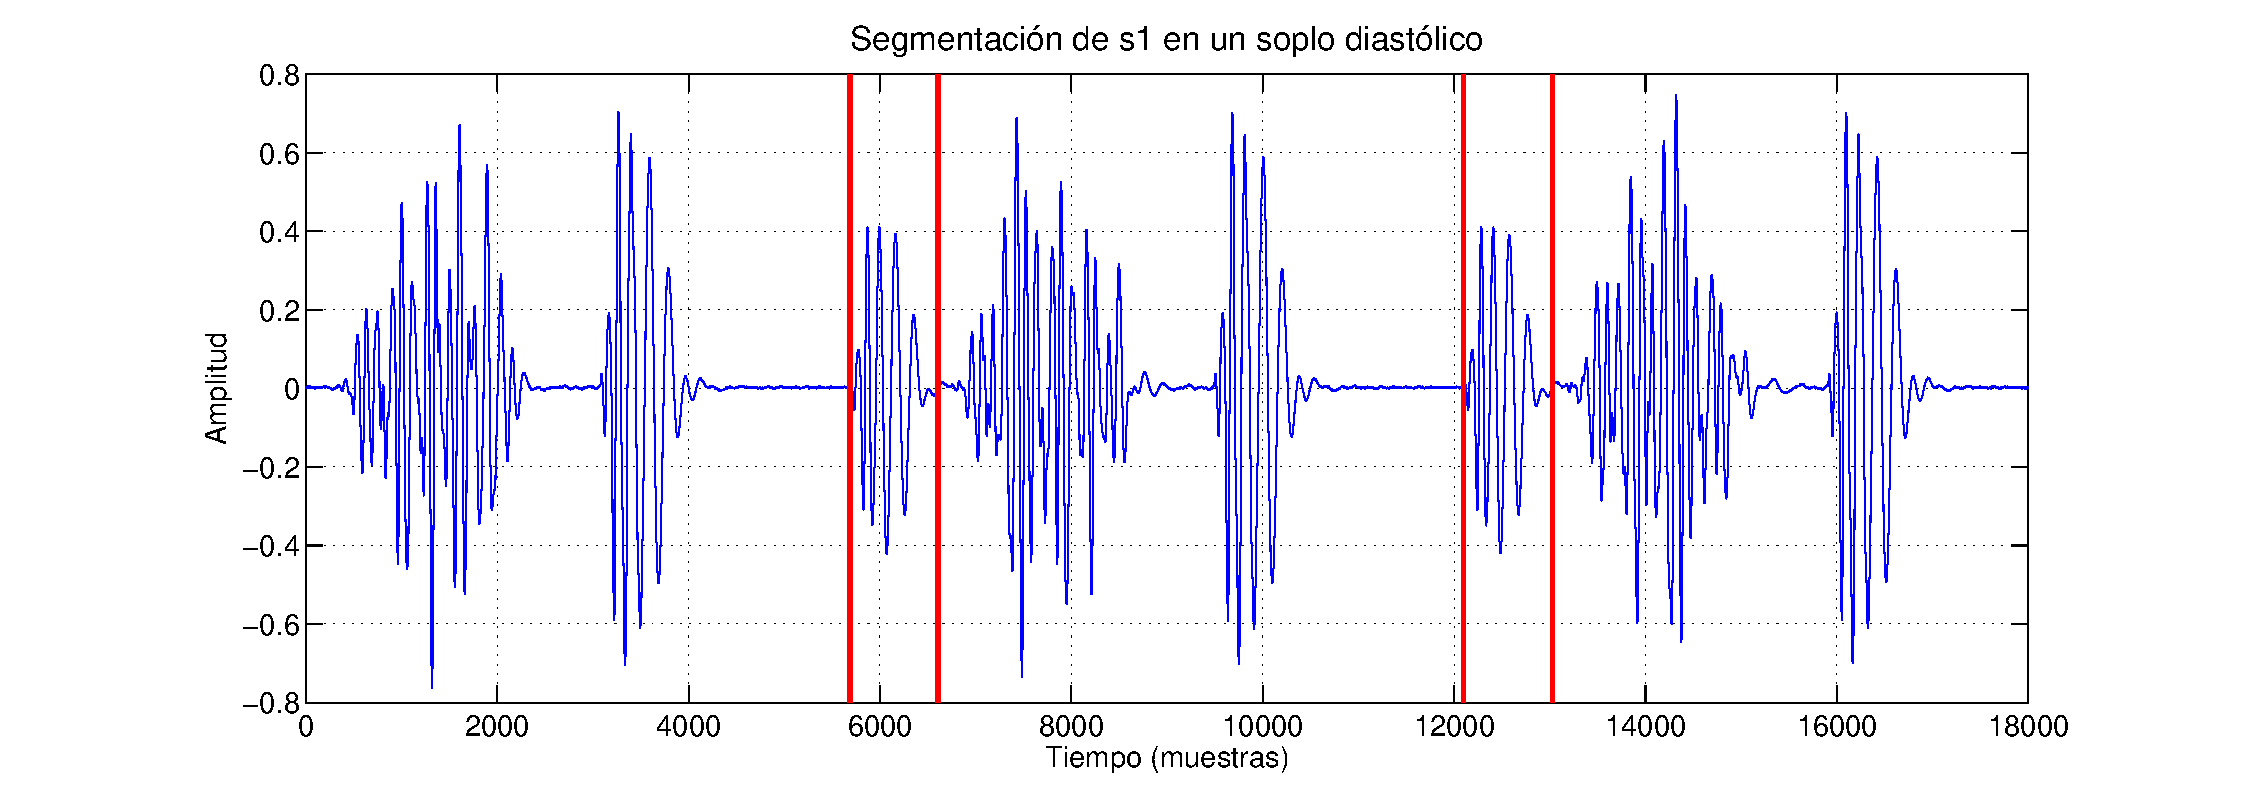
\includegraphics[scale=0.46]{segmentacion.eps}
  \caption{Segmentación del evento cardiaco normal S1 en una señal de audio cardiaco.}
  \label{segment}
\end{figure}
%-------------------------------------------
\section{Descomposición atómica de los eventos (MP)}
Como se ha especificado en el capítulo 3, el proceso de descomposición atómica dado por Matching Pursuit otorga una reconstrucción y compresión aceptables para los eventos cardiacos. La selección de un diccionario \emph{multi-bloques} de Gabor en la descomposición otorga una diversidad atómica en cuanto a frecuencias, posiciones y tamaños de los átomos para la regeneración del evento \cite[]{Nieblas2014}.

\textbf{The Matching Pursuit Toolkit (MPTK)} es una herramienta eficiente en el análisis y síntesis de señales de audio por la técnica Matching Pursuit \cite[]{Krstulovic2006}. La gran ventaja de la herramienta MPTK se basa en la rapidez para calcular las correlaciones (productos internos) entre los átomos del diccionario y las estructuras locales de la señal. Los productos internos son calculados auxiliándose en la FFT y además son actualizados para no re-calcularse (se han preservado en instantes de tiempo anteriores).

En el codificador diseñado para este trabajo de tesis se han realizado las descomposiciones de los eventos cardiacos mediante MPTK y se han seleccionado diccionarios multi-bloques de Gabor como sugiere el trabajo de tesis de \cite{Nieblas2014}. Se trata de dos diccionarios con 4 y 5 bloques respectivamente con las siguientes características que se muestran en la Tabla \ref{dicts}.
% ----------------------------------------------------------------------------------
\begin{table}[h]
\centering
\begin{tabular}{cll}
\hline
\textbf{Parámetros del diccionario}                                                       & \multicolumn{1}{c}{Diccionario 1}                           & \multicolumn{1}{c}{Diccionario 2}                                 \\ \hline
\begin{tabular}[c]{@{}c@{}}Longitudes de las ventanas y \\ átomos (muestras)\end{tabular} & \begin{tabular}[c]{@{}l@{}}64, 128, 256,\\ 512\end{tabular} & \begin{tabular}[c]{@{}l@{}}64, 128, 256,\\ 512, 1024\end{tabular} \\ \hline
\begin{tabular}[c]{@{}c@{}}Tamaños de la FFT\\ (muestras)\end{tabular}                    & \begin{tabular}[c]{@{}l@{}}64, 128, 256,\\ 512\end{tabular} & \begin{tabular}[c]{@{}l@{}}64, 128, 256,\\ 512, 1024\end{tabular} \\ \hline
Tipo de ventana                                                                           & \multicolumn{1}{c}{gaussiana}                               & \multicolumn{1}{c}{gaussiana}                                     \\ \hline
\begin{tabular}[c]{@{}c@{}}Desplazamiento de la\\ ventana (muestras)\end{tabular}         & 8, 16, 24, 32                                               & \begin{tabular}[c]{@{}l@{}}8, 16, 24, 32,\\ 64\end{tabular}       \\ \hline
\end{tabular}
\caption{Características de los diccionarios empleados en la descomposición de los eventos cardiacos del codificador.}
\label{dicts}
\end{table}
% ------------------------------------------------------------------------------

Además, en la Tabla \ref{dicts}, se observa que es conveniente fijar como iguales las longitudes de los átomos y los tamaños de las transformadas rápidas de Fourier (FFT). Esto dará consistencia en las frecuencias atómicas encontradas tras la realización del máximo del producto interno. 

Otro aspecto importante a verificar de los diccionarios es el empalme u \emph{overlap} dado por el corrimiento de la ventana. En este caso las ventanas se irán desplazando por la estructura de la señal en $1/8$ de muestras con relación a su tamaño para calcular las correlaciones correspondientes.

La Figura \ref{MPDecomp} muestra la descomposición mediante MP de un evento cardiaco normal s1 tras realizar 30 iteraciones. Se muestran los primeros 15 átomos seleccionados del análisis ya que presentan mayor amplitud. Se observan en la Figura las diferentes posiciones y frecuencias atómicas (frecuencias de modulación del coseno).
% ------------------------------------------------
\begin{figure}[ht]
  \centering
  \includegraphics[scale=0.38]{MP_decomp.eps}
  \caption{Descomposición MP de un evento cardiaco y muestra de los primeros 15 átomos mayormente correlacionados.}
  \label{MPDecomp}
\end{figure}
% ---------------------------------------------

La Tabla \ref{atoms} muestra el número de eventos y la cantidad de átomos requerida para las descomposiciones Matching Pursuit de las señales de la base de datos. Se observa que la señal del murmullo pansistólico es la que más iteraciones requiere para su representación (392 átomos). Sin duda alguna esta señal presentará menor índice de compresión, dado que la cantidad de átomos es proporcional a la cantidad de bits requeridos para su codificación.

\begin{table}[h]
\centering
\begin{tabular}{lcc}
\hline
\multicolumn{1}{c}{\textbf{Nombre de la señal}} & \textbf{\begin{tabular}[c]{@{}c@{}}Cantidad de \\ eventos\end{tabular}} & \textbf{\begin{tabular}[c]{@{}c@{}}Total de \\ átomos\end{tabular}} \\ \hline
Soplo diastólico                                & 17                                                                      & 264                                                                 \\ \hline
Clic de eyección                                & 19                                                                      & 275                                                                 \\ \hline
Murmullo sistólico temprano                     & 20                                                                      & 365                                                                 \\ \hline
Murmullo sistólico tardío                       & 20                                                                      & 340                                                                 \\ \hline
Chasquido de apertura                           & 19                                                                      & 223                                                                 \\ \hline
S3                                              & 19                                                                      & 197                                                                 \\ \hline
S4                                              & 20                                                                      & 208                                                                 \\ \hline
Murmullo pansistólico                           & 21                                                                      & 392                                                                 \\ \hline
Apertura normal S1                              & 12                                                                      & 130                                                                 \\ \hline
Apertura normal S2                              & 12                                                                      & 172                                                                 \\ \hline
\end{tabular}
	\caption{Cantidad de eventos y número de átomos requeridos en las descomposiciones MP para las señales de la base de datos.}
	\label{atoms}
\end{table}





\section{Modelado y tratamiento de la señal residual (LPC)}

Matching Pursuit, a pesar de ser un algoritmo codicioso (\emph{greedy}) presenta limitantes en cuanto a criterios de selección del número de átomos (iteraciones) o SNR deseada, como se ha mencionado en el capítulo 3. También se ha mencionado que en la práctica el número $N$ de iteraciones nunca es suficiente para representar o retener el 100\% de la energía de la señal analizada, teniendo en la señal residual $R_{M}(t)$ energía aún perceptible para el oído humano dado su comportamiento logarítmico.

En efecto $R_{M}(t)$ presenta correlación muy baja con los átomos de Gabor del diccionario seleccionado, lo cual puede observarse en requerir un gran número de iteraciones sin modelar con éxito esta señal, la cual es considerada por lo tanto como la \emph{parte estocástica} de este codificador de audio.

Es a través de las técnicas de codificación predictiva lineal (LPC) como se ha modelado a la señal residual más silencios del fonocardiograma para el codificador diseñado en esta tesis, parte que se ha establecido que aún contendrá el 1\% de la energía de cada evento del PCG. El criterio de selección de $N$ iteraciones nos da como promedio 10 átomos seleccionados por evento normal y un máximo de 30 átomos por patología o evento de anomalía cardiaca. La Figura \ref{residual} muestra la forma de onda de una señal de soplo diastólico y su señal residual más silencios correspondiente tras realizar el criterio de descomposición antes mencionado.
% ------------------------------------------------
\begin{figure}[ht]
  \centering
  \includegraphics[scale=0.42]{extraccion_residual.eps}
  \caption{Señal de residual y silencios obtenida de un audio cardiaco soplo diastólico.}
  \label{residual}
\end{figure}
% ---------------------------------------------
\subsection{Segmentación del residual}
El análisis LPC de una señal de audio debe realizarse sobre tramos relativamente estacionarios, lo cual reduce la posibilidad de tener cambios abruptos en la autocorrelación y por lo tanto menor cantidad de error en los coeficientes predictores.
Para la señal residual más silencios de audio cardiaco fue necesario tomar tramos de señal de 256 muestras (equivalentes a 32 ms de señal si se considera una frecuencia de muestreo de 8kHz) y posteriormente multiplicarlos por ventanas de análisis tipo \emph{Blackman} para evitar fugas espectrales. 

El empalme u \emph{overlap} de los segmentos analizados fue de 128 muestras (50\%) para asegurar consistencia en la reconstrucción. Se muestra en la Figura \ref{windowing} una descripción gráfica del proceso de segmentación (ventaneo) de la señal residual más silencios cardiacos. 
% ------------------------------------------------
\begin{figure}[ht]
  \centering
  \includegraphics[scale=0.38]{OLA_plot.eps}
  \caption{Ventaneo (segmentación) de la señal residual más silencios.}
  \label{windowing}
\end{figure}
% ---------------------------------------------

 Las tramas de señal obtenidas en el ventaneo son sometidas al análisis LPC, donde será importante extraer los siguientes parámetros para el filtro de síntesis o reconstrucción:
 \begin{itemize}
 	\item Coeficientes predictores $a_{k}$: Calculados mediante la recursión de Levinson por el método de autocorrelación como se mostró en el 			capítulo anterior. El criterio para determinar el número de coeficientes (orden del filtro) se especificará en el siguiente apartado.
	\item Ganancia del filtro predictor: Obtenida para cada trama por la autocorrelación en el instante $t=0$, esto es $\textbf{R}(0)$.
	\item El periodo tonal o pitch: Que se ha obtenido en este trabajo por medio de estimación a través de la función de autocorrelación (ACF) de la 			trama de residual de entrada (máximo de la ACF no ubicado en cero).
 \end{itemize}
 \subsection{Criterios para la determinación del orden $p$ del filtro predictor}
 El filtro predictor lineal es un bloque que se dice \emph{blanquea} o \emph{aplana} el espectro en potencia de la señal de entrada, esto debido a que remueve las correlaciones a corto término.
 La calidad de un filtro predictor se basará en calcular qué tanto es capaz de \emph{aplanar} un espectro en potencia, con lo cual, determinará el grado de tonalidad de un sonido o bien cuánto éste tiende a parecerse a ruido blanco (el cual tiene un espectro plano). Esta medida puede ser obtenida por medio de la \textbf{planitud} o \textbf{aplanamiento espectral}, conocida como \emph{spectral flatness measure} en Inglés. Se denotará en este caso por sus siglas SFM \cite[]{Jayant1974}.
 
 La SFM, $\gamma_{x}^{2}$ se calcula como la razón entre la media geométrica y la media aritmética de la densidad espectral de energía $S_xx(e^{j\omega})$ de una señal de audio:
 %--------------------
 \begin{equation}
 	\gamma_{x}^2 = \frac{\exp\left[\frac{1}{2\pi} \int_{-\pi}^{\pi}\log_{e}S_{xx}(e^{j\omega})d\omega]\right]}{\frac{1}{2\pi}\int_{-\pi}^{\pi}S_{xx}(e^{j\omega})d\omega}.
 \end{equation}
 %--------------------- 
Para la determinación del orden del filtro predictor en la señal residual de audio cardiaco se calculó la SFM promedio de la señal error de cada trama (esta es la salida del predictor lineal) para órdenes predictores $p=1,2,...,100$. Las tramas de audio fueron separadas de acuerdo a si contenían evento cardíaco o presentaban sólo silencio.

De acuerdo a la Figura \ref{sfm}, se ha considerado un aplanamiento aceptable (próximo a volverse constante) a partir de un orden $p=15$ en tramas de silencio cardiaco y tramas con evento respectivamente. 
% ------------------------------------------------
\begin{figure}[ht]
  \centering
  \includegraphics[scale=0.41]{sfm.eps}
  \caption{Medida de planitud espectral promedio de la señal error $e(n)$ para órdenes del filtro predictor desde 1 hasta 100.}
  \label{sfm}
\end{figure}
% ---------------------------------------------
 \subsection{Síntesis/reconstrucción de la señal residual}
 El filtro inverso de reconstrucción IIR por medio de los coeficientes de predicción y la ganancia del filtro predictor reconstruye cada uno de los tramos de señal. Tal como se indicó en el capítulo 4, se presentarán los casos de tener una trama de audio \emph{vocalizada} o \emph{no vocalizada}, excitando al filtro reconstructor con un tren de pulsos separados por el periodo tonal (pitch) en el primer caso y en el segundo mediante ruido blanco gaussiano. 
 
 Una vez regenerados todos los tramos de señal se procede a sintetizar toda la señal de audio cardiaco (contraparte del ventaneo), sumando las partes de los segmentos donde existió el traslape en el ventaneo como se indica en la Figura \ref{OLArecons}. Dicho procedimiento es conocido como \emph{overlap and add (OLA)} en Inglés. 
 % ------------------------------------------------
\begin{figure}[ht]
  \centering
  \includegraphics[scale=0.86]{OLA_recons.pdf}
  \caption{Representación gráfica del procedimiento de síntesis ``overlap and add (OLA)''.}
  \label{OLArecons}
\end{figure}
% ---------------------------------------------
 \subsection{Filtros de pre-énfasis y de-énfasis en LPC}
 La señal de audio cardiaco es pasa-bajas, lo cual indica que en su espectro en potencia a medida que incrementa el rango frecuencial decrece la energía presentada. 
 
 Previo al análisis LPC es conveniente realizar un filtrado de pre-énfasis, cuyo objetivo será realzar las altas frecuencias de la señal y representarlas con una mayor precisión. En la reconstrucción de los segmentos deberá ejecutarse la contraparte de este proceso, el de-énfasis correspondiente que habrá de contrarrestar el efecto. 
 
 Los filtros de pre-énfasis y de-énfasis empleados comúnmente en LPC para los codificadores de voz existentes tienen la siguiente estructura:
 \begin{align}\label{preemph}
 	y(n) = x(n)-a\cdot x(n-1)\\
	y(n) = x(n)+a\cdot x(n-1),
 \end{align}
 donde generalmente se emplea $a=0.9$ en los métodos de predicción lineal.
 
 En la Figura \ref{preem} se muestra la gráfica de la respuesta en frecuencia de los filtros mostrados en \eqref{preemph} y (43), mostrando la parte pasa-altas (pre-énfasis) y pasa-bajas (de-énfasis).
 % ------------------------------------------------
\begin{figure}[ht]
  \centering
  \includegraphics[scale=0.43]{preemp.eps}
  \caption{Filtros de pre-énfasis y de-énfasis usados en la codificación LPC.}
  \label{preem}
\end{figure}
% ---------------------------------------------
\section{Cuantificación}
\subsection{Tipos de cuantificadores}
En la digitalización de una señal de audio está presente un proceso irreversible de compresión con pérdidas como la cuantificación, el cual tiene como objetivo \emph{nivelizar} los parámetros obtenidos para su representación binaria. De manera matemática la cuantificación equivale a sumarle ruido y distorsionar consecuentemente la señal de entrada.

El cuantificador más sencillo de diseñar corresponde a aquella fuente de datos cuya distribución de probabilidad (pdf) es uniforme, sin embargo en la realidad esto no siempre ocurre y es conveniente adaptarlo a una función de distribución de probabilidad no uniforme. 

La Tabla \ref{cuantificadores} define los tipos de cuantificadores con respecto a la dimensión de la fuente de datos de entrada así como a su pdf.
% ---------------------------------------------------------------------------------------------
\begin{table}[h]
\begin{tabular}{|l|l|l|}
\hline
\begin{tabular}[c]{@{}l@{}}Parámetro de la \\ fuente de datos\end{tabular}                             & \begin{tabular}[c]{@{}l@{}}Tipo de \\ cuantificador\end{tabular}     & Características                                                                                                                                \\ \hline
\multirow{2}{*}{\begin{tabular}[c]{@{}l@{}}Función de \\ distribución \\ de probabilidad\end{tabular}} & \begin{tabular}[c]{@{}l@{}}Cuantificador \\ uniforme\end{tabular}    & \begin{tabular}[c]{@{}l@{}}Niveles equidistantes.\\ Implementación sencilla.\end{tabular}                                                      \\ \cline{2-3} 
                                                                                                       & \begin{tabular}[c]{@{}l@{}}Cuantificador no \\ uniforme\end{tabular} & \begin{tabular}[c]{@{}l@{}}Niveles variantes en longitud.\\ Menor distorsión introducida.\end{tabular}                                         \\ \hline
\multirow{2}{*}{Dimensión}                                                                             & Cuantificador escalar                                                & \begin{tabular}[c]{@{}l@{}}Vector unidimensional \\ como fuente de entrada.\end{tabular}                                                       \\ \cline{2-3} 
                                                                                                       & Cuantificador vectorial                                              & \begin{tabular}[c]{@{}l@{}}Cuantificación en bloques \\ (vectores de bits) al agrupar \\ diversas fuentes en \\ una sola entidad.\end{tabular} \\ \hline
\end{tabular}
\caption{Tipos de cuantificadores de acuerdo a las características de la fuente de datos de entrada.}
\label{cuantificadores}
\end{table}


% ---------------------------------------------------------------
\subsection{Diseño de un cuantificador no uniforme}
El cuantificador que introducirá la menor distorsión será aquel que sea diseñado proporcionalmente a la función de distribución de probabilidad de la fuente de entrada. 

El error cuadrado promedio de cuantificación $\sigma_{q}^2$ (MSQE) debe ser el mínimo para presentar la menor distorsión posible tras cuantificar y se define como:
\begin{align}\label{msqe}
	\sigma_{q}^2 = \int_{-\infty}^{\infty} (x-Q(x))^2 f_{X}(x)dx
			 = \sum_{i=1}^{M} \int_{b_{i}-1}^{b_{i}} (x-y_{i})^2 f_{X}(x)dx,
\end{align}
donde $x$ es la fuente de entrada, $Q(x)$ la operación de cuantificación, $f_{X}(x)$ la función de distribución de probabilidad de la fuente, $\{ b_{i}\}_{i=1}^M$ las regiones de decisión y $\{ y_{i}\}_{i=1}^M$ los niveles de reconstrucción (mostrados gráficamente en la Figura \ref{quantz}).
 % ------------------------------------------------
\begin{figure}[ht]
  \centering
  \includegraphics[scale=0.43]{cuantificador.pdf}
  \caption{Regiones de decisión y niveles de reconstrucción de un cuantificador.}
  \label{quantz}
\end{figure}
% ---------------------------------------------
\subsubsection{Algoritmo de Lloyd}
Según lo discutido anteriormente el mejor cuantificador no uniforme surge al tener un modelo probabilístico para la fuente, encontrando los valores $b_{i}$ y $y_{i}$ que minimicen lo definido en la ecuación \eqref{msqe}. La derivación parcial de esta ecuación es un camino para lograr esta minimización, con la cual al resolver para $y_{j}$ se tiene:
%---------------
\begin{equation}\label{nivRec}
	y_{j}=\frac{\int_{b_{j}-1}^{b_{j}} xf_{X}(x)dx}{\int_{b_{j}-1}^{b_{j}} f_{X}(x)dx}.
\end{equation}
%-------------
Teniendo que $\int_{-\infty}^{\infty} xf_{X}(x)dx$ es el valor esperado de la fuente de datos $x$, se define que cada punto a la salida $y_{j}$ para cada intervalo de cuantificación es el centroide de la función de probabilidad en ese intervalo. 

Si se realiza el mismo procedimiento en \eqref{msqe}, ahora para $b_{j}$ (igualando a cero la derivada parcial con respecto a este término) se tiene:
%---------------
\begin{equation}\label{regDec}
	b_{j} = \frac{y_{j+1}+y_{j}}{2}.
\end{equation}
%-------------
Con esto se observa que la región de decisión es simplemente el punto medio de dos niveles de reconstrucción vecinos. Al resolver las ecuaciones \eqref{nivRec} y \eqref{regDec} se obtendrán los valores que minimicen el MSQE definido en \eqref{msqe}, desafortunadamente para resolver $y_{j}$ se requieren los valores $b_{j}$ y $b_{j-1}$ y viceversa. 

El algoritmo de Lloyd, desarrollado por Stuart P. Lloyd describe cómo resolver las ecuaciones \eqref{nivRec} y \eqref{regDec} de manera iterativa, obteniendo los valores $b_{j}$ y $y_{j}$ a base de simetría y suponiendo los valores para la primer región de decisión $b_{0}$ como cero, así como suponiendo que la última región $b_{\frac{M}{2}}$ es el valor más grande que puede tener la entrada. 

\subsection{Cuantificación de los parámetros extraídos de los modelados}

Para el desarrollo del códec de audio propuesto se han cuantificado aquellos parámetros que estén en formato de punto flotante para convertirse en enteros con signo. Esto garantizará la correcta representación de los mismos con el menor número de bits posibles. Es necesario determinar ahora de los parámetros extraídos del PCG de los modelados MP y LPC, cuáles es necesario cuantificar y cuáles será necesario codificar directamente (ya que son enteros con signo).
 % ------------------------------------------------
\begin{figure}[ht]
  \centering
  \includegraphics[scale=0.48]{params_cuant.png}
  \caption{Parámetros extraídos de los modelados MP y LPC para el códec. Se indican los parámetros necesarios de cuantificar.}
  \label{params}
\end{figure}
% ---------------------------------------------

De acuerdo a lo observado en la Figura \ref{params}, habrá que diseñar 4 cuantificadores para el códec, correspondientes a las amplitudes y fases de los átomos seleccionados en MP, los coeficientes de líneas espectrales diferenciales (LSFD, obtenidos a través de los coeficientes predictores) y las ganancias de los filtros de predicción de LPC. El primer paso corresponderá a observar las funciones de distribución de probabilidad (pdf) de las variables para posteriormente determinar sus cuantificadores optimizados mediante el algoritmo de Lloyd.

Se han realizado los histogramas normalizados para determinar las funciones de probabilidad de las amplitudes y fases atómicas extraídas desde MPTK para las señales de la base de datos.
 % ------------------------------------------------
\begin{figure}[ht]
  \centering
  \includegraphics[scale=0.42]{histograma_amplitudesFases.eps}
  \caption{Histogramas normalizados (pdf) para las amplitudes y fases de los átomos extraídos en las descomposiciones.}
  \label{histAmpPh}
\end{figure}
% ---------------------------------------------

 % ------------------------------------------------
\begin{figure}[h!]
  \centering
  \includegraphics[scale=0.42]{histograma_LSFDGanancia.eps}
  \caption{Histogramas normalizados (pdf) para los coeficientes LSFD y ganancias del filtro predictor.}
  \label{histLSFD}
\end{figure}
% ---------------------------------------------

En la Figura \ref{histAmpPh} se observa que la distribución de probabilidad de las fases de los átomos es de manera uniforme en el intervalo $[-\pi,\pi]$, siendo necesario diseñar un cuantificador sencillo para esta variable. En el caso de la amplitud se procederá a diseñar con el algoritmo de Lloyd un cuantificador no uniforme basado en su pdf.

Se observa un comportamiento no uniforme en las funciones de probabilidad obtenidas a través de los histogramas de los coeficientes LSFD y ganancia del filtro predictor, esto según la Figura \ref{histLSFD}. De igual manera que con la amplitud, mediante el método de Lloyd se realizará el diseño de estos cuantificadores no uniformes optimizados.

\subsection{Cuantificación de los coeficientes de predicción}
Como se ha manejado anteriormente, los coeficientes obtenidos para la predicción lineal son bastante sensibles a la inestabilidad, por lo tanto su cuantificación no es realizable de manera directa para su transmisión, ya que la distorsión introducida afectaría en gran medida en la síntesis de la señal \cite[]{Noah1984}.

Sin embargo, existen otras representaciones equivalentes de los coeficientes predictores LPC empleadas en algunos vocoders diseñados en la literatura, con las cuales puede realizarse la cuantificación presentando la menor distorsión posible:

\begin{itemize} 
	\item \textbf{Coeficientes reflectores o PARCORS}: Se obtienen directamente a partir de la recursión de Levinson a la par de los coeficientes 				predictores.
	\item \textbf{Coeficientes de relación log-área (log-area ratios o LAR)}: Los coeficientes reflectores $k_{i}$ pueden sufrir transformaciones para expandir su región en el plano polar \cite[]{Viswanathan1975}. 
	
	Una de estas transformaciones es calculada como el logaritmo de la razón de la suma y resta del $i$-ésimo coeficiente reflector, en una representación conocida como relación log-área (LAR), esto es: $$LAR_{i}=\log\frac{1+k_{i}}{1-k_{i}}.$$
	\item \textbf{Pares o frecuencias de líneas espectrales (line spectrum pairs/frequencies, LSF)}: \cite{Itakura1975}, encontró que el polinomio del filtro predictor $A(z)$ tiene	una representación equivalente a partir de un par de polinomios:
					$$A(z) = 0.5[P(z)+Q(z)]$$
					$$P(z) = A(z)+z^{-(p+1)}A(z^{-1})$$
					$$Q(z) = A(z)-z^{-(p+1)}A(z^{-1}).$$
			Las raíces de $P(z)$ y $Q(z)$ ocurren en pares conjugados y se les denomina \emph{frecuencias} o \emph{pares} de 						líneas espectrales.			
	\item \textbf{Pares o frecuencias de líneas espectrales diferenciales (LSFD's)}: \cite{Soong1984a} explotaron la correlación entre LSF's sucesivos, para ello cuantificaron las diferencias entre éstos. A tal representación equivalente se le conoce como LSF diferenciales ó LSFD's:
			$$LSFD_{i}=LSF_{i+1}-LSF_{i}.$$
\end{itemize}
Seleccionar la representación LPC adecuada en el diseño del codificador será una medida que intervendrá en la calidad de la reconstrucción de la señal. La distorsión espectral (medida en decibeles) es una medida que indica la cantidad de degradación del espectro en potencia de la señal analizada tras seleccionar alguna representación equivalente de las antes mencionadas y haber cuantificado. 

 Se define como la distorsión espectral $D_{i}$ común entre dos tramas de audio a la siguiente expresión:
 \begin{equation}\label{spectralDisort}
 	D_{i} = \sqrt{ \frac{1}{f_{s}} \int_{0}^{f_{s}} [10\log_{10}(P_{i}(f))-10\log_{10}(\widehat{P}_{i}(f))]^{2} df  },
 \end{equation}
 donde $f_{s}$ es la frecuencia de muestreo en Hz,  $P_{i}(f)$ y $\widehat{P}_{i}(f)$ son los espectros de potencia LPC de las $i$-ésimas tramas, dados por: $$ P_{i}(f)=\frac{1}{\lvert A_{i}(\exp(j2\pi f/f_{s})) \rvert^{2}}$$
 $$ \widehat{P}_{i}(f)=\frac{1}{\lvert \widehat{A}_{i}(\exp(j2\pi f/f_{s})) \rvert^{2}},$$
 
donde $A_{i}(z)$ y $\widehat{A}_{i}(z)$ son los polinomios LPC originales y cuantificados de la $i$-ésima trama respectivamente. 

La distorsión espectral es evaluada para todas las tramas en los datos experimentales y su valor promedio es calculado. Este valor es la distorsión asociada a un cuantificador en particular.

Los coeficientes seleccionados son los que introduzcan menores cantidades de distorsión espectral tras reconstruir la señal después de su cuantificación, para ello se ha calculado $D_{i}$ en las 288 tramas resultantes de 32ms (256 muestras) de la señal soplo diastólico para los coeficientes LPC reflectores ($k_{i}$), log-area (LAR), LSF y LSFD realizando la cuantificación no uniforme con un cuantificador optimizado de Lloyds para cada caso. Los resultados de este procedimiento se muestran en la Figura \ref{spectrDis}.
 % ------------------------------------------------
\begin{figure}[h!]
  \centering
  \includegraphics[scale=0.48]{spectral_disortion.eps}
  \caption{Distorsión espectral común por el ruido de cuantificación aplicada a diferentes representaciones equivalentes LPC.}
  \label{spectrDis}
\end{figure}

% ---------------------------------------------

Tras observar la Figura \ref{spectrDis}, se ha decidido el emplear coeficientes del tipo LSFD ya que introducen menores niveles de distorsión espectral tras ser cuantificados. De igual forma, disminuyen el rango dinámico empleado para las regiones de decisión del cuantificador, permitiendo representar con menos bits a cada uno de estos coeficientes. 

\section{Representación en bits de los parámetros de codificación}

Una vez diseñados los cuantificadores optimizados de los parámetros requeridos para codificar es conveniente determinar el número de bits para representar cada uno de ellos. De igual manera, se requiere conocer dicha cantidad para aquellos parámetros que son enteros con signo y no requerirán cuantificación. Estos conceptos son mostrados en la Tabla \ref{Nbits}.
\begin{table}[h]
\centering
\begin{tabular}{@{}lcl@{}}
\toprule
\multicolumn{3}{c}{Parámetros de la parte determinística (MP)}                           \\ \midrule
Parámetro extraído    & \multicolumn{1}{l}{Núm. bits requeridos/átomo} & Tipo de cuantificador \\ \midrule
Amplitud atómica      & 8                                        & No uniforme           \\ \midrule
Longitud atómica      & 3                                        & Sin cuantificador     \\ \midrule
Fase atómica          & 8                                        & Uniforme              \\ \midrule
Posición atómica      & 8                                        & Sin cuantificador     \\ \midrule
Frecuencia atómica    & 6                                        & Sin cuantificador     \\ \midrule
\multicolumn{3}{c}{Parámetros de la parte estocástica (LPC)}                            \\ \midrule
Parámetro extraído    & \multicolumn{1}{l}{Núm. bits requeridos/segmento} & Tipo de cuantificador \\ \midrule
Ganancia del filtro   & 4                                        & No uniforme           \\ \midrule
Periodo tonal (Pitch) & 8                                        & Sin cuantificador     \\ \midrule
LSFD                  & 7                                        & No uniforme          
\end{tabular}
	\caption{Número de bits requeridos por parámetro y tipo de cuantificación realizada.}
	\label{Nbits}
\end{table}


A continuación se enlistan las razones por las cuales algunos de los parámetros enlistados de la Tabla \ref{Nbits} no requirieron el diseño de un cuantificador:
 \begin{itemize}
 	\item Las \emph{longitudes} de los átomos (que son equivalentes a las longitudes de las ventanas) fueron pre-seleccionadas con el tipo de 			diccionario empleado para la descomposición y corresponden a 64, 128, 256, 512 y 1024 muestras. Se trata de 5 cantidades que pueden 		representarse con sólo 3 bits.
	\item Con la elección del diccionario también se permitió preseleccionar el desplazamiento de las ventanas gaussianas, el cual fue a 1/8 de 			sus longitudes. Por ello las \emph{posiciones} de los átomos son múltiplos de 8 que pueden representarse con enteros de 8 bits sin 			signo.
	\item  Las \emph{frecuencias} atómicas pudieron convertirse a enteros tras multiplicar su valor decimal por el tamaño de la FFT, cantidad que 			es equivalente al tamaño de las ventanas en el diccionario. De acuerdo a su rango dinámico se consideraron necesarios 6 bits para su 			representación. 
	\item El periodo tonal o \emph{pitch} fue observado en cuanto a rango dinámico. Al ser necesario su valor en muestras para la implementación 		éste debe ser un entero. Se concluyó que 7 bits son necesarios para representar cada uno de sus valores.
 \end{itemize}
 
 \section{Codificación de los fonocardiogramas y porcentajes de compresión obtenidos}
Para la evaluación del desempeño del codificador diseñado es necesario calcular las tasas de compresión al implementarlo en el catálogo de señales de prueba antes mencionado. Se ha decidido calcular el porcentaje de compresión $C_{r}$ como una relación entre bits utilizados por el codificador y bits empleados para codificar a velocidades de transmisión de $R_{b}=64$ y $R_{b}=128$ kilobits por segundo (kbps), esto es: $$ C_{r}= \frac{ cantidad~de~bits~codificador}{cantidad~de~bits~R_{b}}.$$

La Tabla \ref{comRat} muestra los porcentajes de compresión $C_{r}$ calculados para las señales de la base Litman por el codificador, de igual manera se indican los bits que se requieren para codificar cada una de las muestras de audio cardiaco. Estos porcentajes son en proporción a las cantidades de átomos obtenidas en la Tabla \ref{atoms}.
\begin{table}[h]
\centering
\begin{tabular}{l|c|c|c}
\hline
\multicolumn{1}{|l|}{\multirow{2}{*}{Nombre de la señal}} & \multicolumn{2}{c|}{Porcentaje de compresión (\%)} & \multicolumn{1}{l|}{\multirow{2}{*}{\begin{tabular}[c]{@{}l@{}}Bits requeridos\\ por el codificador\end{tabular}}} \\ \cline{2-3}
\multicolumn{1}{|l|}{}                                    & @128 kpbs     & \multicolumn{1}{l|}{@ 64 kbps}     & \multicolumn{1}{l|}{}                                                                                              \\ \hline
Soplo diastólico                                          & 93.24        & 86.47                             & 39,818                                                                                                             \\ \hline
Clic de eyección                                          & 93.88        & 87.68                             & 39,115                                                                                                             \\ \hline
Murmullo sistólico temprano                               & 93.35        & 86.70                             & 43,301                                                                                                             \\ \hline
Murmullo sistólico tardío                                 & 93.30        & 86.61                             & 44,333                                                                                                             \\ \hline
Chasquido de apertura                                     & 94.06        & 88.13                             & 38,077                                                                                                             \\ \hline
S3                                                        & 93.99        & 87.98                             & 38,385                                                                                                             \\ \hline
S4                                                        & 94.06        & 88.16                             & 39,031                                                                                                             \\ \hline
Murmullo pansistólico                                     & 93.00        & 86.00                             & 47,358                                                                                                             \\ \hline
División normal de S1                                     & 94.49        & 88.98                             & 31,602                                                                                                             \\ \hline
División normal de S2                                     & 94.21        & 88.43                             & 34,005                                                                                                            
\end{tabular}
	\caption{Porcentajes de compresión y bits requeridos para el codificador diseñado en las señales de prueba.}
	\label{comRat}
\end{table}

\section{Pruebas en la reconstrucción de los fonocardiogramas}
Tal y como se ha definido en el diagrama de la Figura \ref{diagDecod}, los procedimientos de decodificación dan lugar a la reconstrucción de la señal $\hat{x}(t)$, la cual necesita ser comparada con el fonocardiograma de entrada $x(t)$. 

Para esto la Figura \ref{pcgRecons} muestra las formas de onda de la señal original y la señal reconstruida tras aplicar el procedimiento de codificación planteado en el caso del murmullo sistólico tardío, las cuales se observan muy similares.
 % ------------------------------------------------
\begin{figure}[ht]
  \centering
  \includegraphics[scale=0.45]{pcgRecons.eps}
  \caption{Formas de onda original y reconstruida por el códec para un ciclo de un murmullo sistólico tardío.}
  \label{pcgRecons}
\end{figure}
% ---------------------------------------------
\subsection{Coeficiente de correlación}
A pesar de que el codificador diseñado ha mostrado buenos resultados en cuanto a replicar la forma de onda es necesario medir el grado de intensidad que guardan las variables $x(t)$ y $\hat{x}(t)$ matemáticamente \cite[]{Senhadji1995}. 

El coeficiente de correlación $\rho_{x,\hat{x}}$ es una medida que cuantifica y describe esta relación por medio de la razón de las covarianzas entre éstas dos variables, esto es:
\begin{equation}
	\rho_{x,\hat{x}} = \frac{\sigma_{x\hat{x}}}{\sigma_{x}\sigma_{\hat{x}}} = \frac{E[(x-\mu_{x})(\hat{x}-\mu_{\hat{x}})]}{\sigma_{x}\sigma_{\hat{x}}},
\end{equation}
donde $\sigma_{x\hat{x}}$ es la covarianza de las variables $x$ y $\hat{x}$; $\sigma_{x}$ es la desviación estándar de la variable $x$ y $\sigma_{\hat{x}}$ es la desviación estándar de la variable $\hat{x}$ respectivamente.
 
 Se calculó el coeficiente de correlación después de codificar y reconstruir cada una de las señales analizadas en la base de datos de la Tabla \ref{wavsounds} con respecto a las señales reconstruidas. Los resultados se muestran en la Tabla \ref{corrCoefs}.

\begin{table}[h]
\centering
\begin{tabular}{l|c}
\hline
\multicolumn{1}{|l|}{\multirow{2}{*}{Nombre de la señal}} & \multicolumn{1}{l|}{\multirow{2}{*}{\begin{tabular}[c]{@{}l@{}}Coeficiente de \\ correlación\end{tabular}}} \\
\multicolumn{1}{|l|}{}                                    & \multicolumn{1}{l|}{}                                                                                       \\ \hline
Soplo diastólico                                          & 0.9697                                                                                                      \\ \hline
Clic de eyección                                          & 0.9724                                                                                                      \\ \hline
Murmullo sistólico temprano                               & 0.9335                                                                                                      \\ \hline
Murmullo sistólico tardío                                 & 0.9330                                                                                                      \\ \hline
Chasquido de apertura                                     & 0.9406                                                                                                      \\ \hline
S3                                                        & 0.9614                                                                                                      \\ \hline
S4                                                        & 0.9638                                                                                                      \\ \hline
Murmullo pansistólico                                     & 0.9648                                                                                                      \\ \hline
División normal de S1                                     & 0.9634                                                                                                      \\ \hline
División normal de S2                                     & 0.9675                                                                                                    
\end{tabular}
	\caption{Coeficientes de correlación de las señales reconstruidas comparadas con los audios originales.}
	\label{corrCoefs}
\end{table}

Según lo observado en la Tabla \ref{corrCoefs}, los audios reconstruidos han mostrado fuerte correlación (cercana a 1) en comparación a los fonocardiogramas originales, lo cual indica dependencia lineal y buenos resultados para el codificador. 

\subsection{Raíz cuadrada de la diferencia cuadrática media (Percent Root-mean-square Difference, PRD)}

La calidad de reconstrucción en un esquema de compresión de señales PCG se ha obtenido comúnmente por medio de una cantidad denominada \emph{Raíz cuadrada de la diferencia cuadrática media}, lo cual es realmente una medida del porcentaje de degradación de una señal tras sufrir cambios en el proceso de compresión \cite[]{Blanco-Velasco2005}. Suponiendo las mismas variables, $x$ como el fonocardiograma original y $\hat{x}$ como el PCG reconstruido posterior a la codificación se define su PRD como:
\begin{equation}
	PRD = \sqrt{ \frac{\displaystyle \sum_{i=1}^{N} (x_{i}-\hat{x}_{i})^2}{\displaystyle \sum_{i=1}^{N} (x_{i}-\mu_{x})^2} } \times 100,
\end{equation}

donde $\mu_{x}$ es la media o valor esperado de la variable $x$.

Es evidente que la señal $x$ habrá sido exitosamente reconstruida tras aplicar el esquema de compresión si el PRD calculado es lo más reducido posible. 

La Tabla \ref{PRD} muestra los valores de la raíz cuadrada de la diferencia cuadrática media calculados para las señales reconstruidas de la base de datos tomada comparándolas con las señales reconstruidas por el codificador propuesto, observando muy buenos resultados debido a su bajo valor de degradación (no rebasa el 3\% en ninguno de los casos).
\begin{table}[h]
\centering
\begin{tabular}{l|c}
\hline
\multicolumn{1}{|l|}{\multirow{2}{*}{Nombre de la señal}} & \multicolumn{1}{c|}{\multirow{2}{*}{PRD}} \\
\multicolumn{1}{|l|}{}                                    & \multicolumn{1}{c|}{}                     \\ \hline
Soplo diastólico                                          & 2.50                                     \\ \hline
Clic de eyección                                          & 2.38                                     \\ \hline
Murmullo sistólico temprano                               & 2.33                                     \\ \hline
Murmullo sistólico tardío                                 & 2.41                                     \\ \hline
Chasquido de apertura                                     & 2.15                                     \\ \hline
S3                                                        & 2.87                                     \\ \hline
S4                                                        & 2.77                                     \\ \hline
Murmullo pansistólico                                     & 2.74                                     \\ \hline
División normal de S1                                     & 2.77                                     \\ \hline
División normal de S2                                     & 2.61                                    
\end{tabular}
	\caption{Cálculo de la raíz cuadrada de la diferencia cuadrática media (PRD) para las señales de la base de datos.}
	\label{PRD}
\end{table}



} }%
%BeginExpansion

\chapter{Conformación del códec propuesto}\label{capit:cap5}
\vspace{-2.0325ex}%
\noindent
\rule{\textwidth}{0.5pt}
\vspace{-5.5ex}% 
\newcommand{\pushline}{\Indp}% Indent puede ir o no :p

Una vez definidos los conceptos necesarios para el modelado de la parte determinística (Matching Pursuit) y la parte estocástica (Codificación predictiva lineal) del codificador de audio propuesto para este trabajo de tesis, es conveniente mostrar los elementos necesarios para diseñarlo. Para ello, se tomarán los parámetros necesarios de ambos modelados que reconstruyan con precisión la señal de audio cardiaco. 

Una vez obtenidos los parámetros necesarios para conformar el códec es necesario cuantificarlos, este requerimiento es necesario en el sentido de representarlos por medio de palabras código para ser almacenados. La cuantificación es un proceso irreversible de compresión con pérdidas en la codificación de toda señal de audio, el cual por lo tanto debe ser cuidadosamente analizado para que no se distorsionen en gran medida los parámetros que se han cuantificado.

En este capítulo se muestran los pasos necesarios para la conformación del codificador de audio cardiaco; la extracción de los parámetros y su cuantificación. Por último se definirán las tasas de compresión y medidas de distorsión generadas por las señales codificadas para comparar el códec de manera objetiva. 

\section{Estructura del codificador-decodificador propuesto}
Para el desarrollo, modelado y pruebas realizadas al codificador y otros procesos durante este trabajo de tesis se han seleccionado 10 señales de audio cardiaco con duración de 5 segundos desde una base de datos disponible en el sitio web oficial de Litman \copyright, desarrolladores de estetoscopios y otras herramientas de diagnóstico clínico \cite[]{LitmannBase}.

 Se han obtenido las señales indicadas en la Tabla \ref{wavsounds} en formato .wav muestreadas a 11,025 Hz.  Por cuestiones de compatibilidad con los diccionarios en la descomposición las señales han sido remuestreadas a 8,000 Hz.
%--------------------------------------------------------------
\begin{table}[h]
\centering
\begin{tabular}{l}
\hline
\multicolumn{1}{c}{\textbf{Nombre de la señal}}     \\ \hline
División normal del primer ruido (Normal Split S1)  \\ \hline
División normal del segundo ruido (Normal Split S2) \\ \hline
S3                                                  \\ \hline
S4                                                  \\ \hline
Murmullo sistólico temprano (Early Systolic Murmur) \\ \hline
Murmullo sistólico tardío (Late Systolic Murmur)    \\ \hline
Clic de eyección (Ejection Click)                   \\ \hline
Chasquido de apertura (Opening Snap)                \\ \hline
Murmullo pansistólico (Pansystolic Murmur)          \\ \hline
Soplo diastólico (Diastolic Rumble)                 \\ \hline
\end{tabular}
\caption{Sonidos de la base del sitio web Littman \copyright~analizados en este trabajo de tesis. Tomados de \cite[]{LitmannBase}.}
\label{wavsounds}
\end{table}
 %--------------------------------------------------------------
 
El codificador de audio propuesto para este trabajo de tesis consta de los dos modelados matemáticos básicos mostrados en los capítulos anteriores (MP y LPC). 

La Figura \ref{diagEncod} muestra la estructura del codificador diseñado, cuyas etapas serán brevemente explicadas en esta sección. El canal de distribución y/o almacenamiento no será referido durante este trabajo.

Por otra parte, en la Figura \ref{diagDecod} se muestra el procedimiento de decodificación, cuyas etapas son las necesarias para la conformación de la señal de audio reconstruida, la cual será analizada en términos de porcentaje de compresión, distorsión y niveles de error cuadrático medidos desde la señal de audio cardiaco original. 
% ------------------------------------------------
\begin{figure}[h!]
  \centering
  \includegraphics[scale=0.46]{codificador.png}
  \caption{Estructura del codificador para audio cardiaco propuesto.}
  \label{diagEncod}
\end{figure}
% ---------------------------------------------
% ------------------------------------------------
\begin{figure}[h!]
  \centering
  \includegraphics[scale=0.46]{decodificador.png}
  \caption{Estructura del decodificador para audio cardiaco propuesto.}
  \label{diagDecod}
\end{figure}
% ---------------------------------------------
\section{Segmentación de los eventos cardiacos}
El proceso de codificación de audio cardiaco inicia con la \emph{segmentación}, tarea que consiste en extraer los instantes de tiempo (ya sea en segundos o en muestras) donde comienza (\emph{onset}) y termina (\emph{offset}) un sonido o evento cardiaco. La precisión en la localización de estos intervalos es importante\footnote{Esto es, que los valores obtenidos difieran en pocas muestras.}. El diseño del algoritmo automático de segmentación no es parte de los objetivos de este trabajo de tesis, por lo tanto se ha realizado de manera manual.
%-------------------------------------------------
\begin{figure}[ht]
  \centering
  \includegraphics[scale=0.46]{segmentacion.eps}
  \caption{Segmentación del evento cardiaco normal S1 en una señal de audio cardiaco.}
  \label{segment}
\end{figure}
%-------------------------------------------
\section{Descomposición atómica de los eventos (MP)}
Como se ha especificado en el capítulo 3, el proceso de descomposición atómica dado por Matching Pursuit otorga una reconstrucción y compresión aceptables para los eventos cardiacos. La selección de un diccionario \emph{multi-bloques} de Gabor en la descomposición otorga una diversidad atómica en cuanto a frecuencias, posiciones y tamaños de los átomos para la regeneración del evento \cite[]{Nieblas2014}.

\textbf{The Matching Pursuit Toolkit (MPTK)} es una herramienta eficiente en el análisis y síntesis de señales de audio por la técnica Matching Pursuit \cite[]{Krstulovic2006}. La gran ventaja de la herramienta MPTK se basa en la rapidez para calcular las correlaciones (productos internos) entre los átomos del diccionario y las estructuras locales de la señal. Los productos internos son calculados auxiliándose en la FFT y además son actualizados para no re-calcularse (se han preservado en instantes de tiempo anteriores).

En el codificador diseñado para este trabajo de tesis se han realizado las descomposiciones de los eventos cardiacos mediante MPTK y se han seleccionado diccionarios multi-bloques de Gabor como sugiere el trabajo de tesis de \cite{Nieblas2014}. Se trata de dos diccionarios con 4 y 5 bloques respectivamente con las siguientes características que se muestran en la Tabla \ref{dicts}.
% ----------------------------------------------------------------------------------
\begin{table}[h]
\centering
\begin{tabular}{cll}
\hline
\textbf{Parámetros del diccionario}                                                       & \multicolumn{1}{c}{Diccionario 1}                           & \multicolumn{1}{c}{Diccionario 2}                                 \\ \hline
\begin{tabular}[c]{@{}c@{}}Longitudes de las ventanas y \\ átomos (muestras)\end{tabular} & \begin{tabular}[c]{@{}l@{}}64, 128, 256,\\ 512\end{tabular} & \begin{tabular}[c]{@{}l@{}}64, 128, 256,\\ 512, 1024\end{tabular} \\ \hline
\begin{tabular}[c]{@{}c@{}}Tamaños de la FFT\\ (muestras)\end{tabular}                    & \begin{tabular}[c]{@{}l@{}}64, 128, 256,\\ 512\end{tabular} & \begin{tabular}[c]{@{}l@{}}64, 128, 256,\\ 512, 1024\end{tabular} \\ \hline
Tipo de ventana                                                                           & \multicolumn{1}{c}{gaussiana}                               & \multicolumn{1}{c}{gaussiana}                                     \\ \hline
\begin{tabular}[c]{@{}c@{}}Desplazamiento de la\\ ventana (muestras)\end{tabular}         & 8, 16, 24, 32                                               & \begin{tabular}[c]{@{}l@{}}8, 16, 24, 32,\\ 64\end{tabular}       \\ \hline
\end{tabular}
\caption{Características de los diccionarios empleados en la descomposición de los eventos cardiacos del codificador.}
\label{dicts}
\end{table}
% ------------------------------------------------------------------------------

Además, en la Tabla \ref{dicts}, se observa que es conveniente fijar como iguales las longitudes de los átomos y los tamaños de las transformadas rápidas de Fourier (FFT). Esto dará consistencia en las frecuencias atómicas encontradas tras la realización del máximo del producto interno. 

Otro aspecto importante a verificar de los diccionarios es el empalme u \emph{overlap} dado por el corrimiento de la ventana. En este caso las ventanas se irán desplazando por la estructura de la señal en $1/8$ de muestras con relación a su tamaño para calcular las correlaciones correspondientes.

La Figura \ref{MPDecomp} muestra la descomposición mediante MP de un evento cardiaco normal s1 tras realizar 30 iteraciones. Se muestran los primeros 15 átomos seleccionados del análisis ya que presentan mayor amplitud. Se observan en la Figura las diferentes posiciones y frecuencias atómicas (frecuencias de modulación del coseno).
% ------------------------------------------------
\begin{figure}[ht]
  \centering
  \includegraphics[scale=0.38]{MP_decomp.eps}
  \caption{Descomposición MP de un evento cardiaco y muestra de los primeros 15 átomos mayormente correlacionados.}
  \label{MPDecomp}
\end{figure}
% ---------------------------------------------

La Tabla \ref{atoms} muestra el número de eventos y la cantidad de átomos requerida para las descomposiciones Matching Pursuit de las señales de la base de datos. Se observa que la señal del murmullo pansistólico es la que más iteraciones requiere para su representación (392 átomos). Sin duda alguna esta señal presentará menor índice de compresión, dado que la cantidad de átomos es proporcional a la cantidad de bits requeridos para su codificación.

\begin{table}[h]
\centering
\begin{tabular}{lcc}
\hline
\multicolumn{1}{c}{\textbf{Nombre de la señal}} & \textbf{\begin{tabular}[c]{@{}c@{}}Cantidad de \\ eventos\end{tabular}} & \textbf{\begin{tabular}[c]{@{}c@{}}Total de \\ átomos\end{tabular}} \\ \hline
Soplo diastólico                                & 17                                                                      & 264                                                                 \\ \hline
Clic de eyección                                & 19                                                                      & 275                                                                 \\ \hline
Murmullo sistólico temprano                     & 20                                                                      & 365                                                                 \\ \hline
Murmullo sistólico tardío                       & 20                                                                      & 340                                                                 \\ \hline
Chasquido de apertura                           & 19                                                                      & 223                                                                 \\ \hline
S3                                              & 19                                                                      & 197                                                                 \\ \hline
S4                                              & 20                                                                      & 208                                                                 \\ \hline
Murmullo pansistólico                           & 21                                                                      & 392                                                                 \\ \hline
Apertura normal S1                              & 12                                                                      & 130                                                                 \\ \hline
Apertura normal S2                              & 12                                                                      & 172                                                                 \\ \hline
\end{tabular}
	\caption{Cantidad de eventos y número de átomos requeridos en las descomposiciones MP para las señales de la base de datos.}
	\label{atoms}
\end{table}





\section{Modelado y tratamiento de la señal residual (LPC)}

Matching Pursuit, a pesar de ser un algoritmo codicioso (\emph{greedy}) presenta limitantes en cuanto a criterios de selección del número de átomos (iteraciones) o SNR deseada, como se ha mencionado en el capítulo 3. También se ha mencionado que en la práctica el número $N$ de iteraciones nunca es suficiente para representar o retener el 100\% de la energía de la señal analizada, teniendo en la señal residual $R_{M}(t)$ energía aún perceptible para el oído humano dado su comportamiento logarítmico.

En efecto $R_{M}(t)$ presenta correlación muy baja con los átomos de Gabor del diccionario seleccionado, lo cual puede observarse en requerir un gran número de iteraciones sin modelar con éxito esta señal, la cual es considerada por lo tanto como la \emph{parte estocástica} de este codificador de audio.

Es a través de las técnicas de codificación predictiva lineal (LPC) como se ha modelado a la señal residual más silencios del fonocardiograma para el codificador diseñado en esta tesis, parte que se ha establecido que aún contendrá el 1\% de la energía de cada evento del PCG. El criterio de selección de $N$ iteraciones nos da como promedio 10 átomos seleccionados por evento normal y un máximo de 30 átomos por patología o evento de anomalía cardiaca. La Figura \ref{residual} muestra la forma de onda de una señal de soplo diastólico y su señal residual más silencios correspondiente tras realizar el criterio de descomposición antes mencionado.
% ------------------------------------------------
\begin{figure}[ht]
  \centering
  \includegraphics[scale=0.42]{extraccion_residual.eps}
  \caption{Señal de residual y silencios obtenida de un audio cardiaco soplo diastólico.}
  \label{residual}
\end{figure}
% ---------------------------------------------
\subsection{Segmentación del residual}
El análisis LPC de una señal de audio debe realizarse sobre tramos relativamente estacionarios, lo cual reduce la posibilidad de tener cambios abruptos en la autocorrelación y por lo tanto menor cantidad de error en los coeficientes predictores.
Para la señal residual más silencios de audio cardiaco fue necesario tomar tramos de señal de 256 muestras (equivalentes a 32 ms de señal si se considera una frecuencia de muestreo de 8kHz) y posteriormente multiplicarlos por ventanas de análisis tipo \emph{Blackman} para evitar fugas espectrales. 

El empalme u \emph{overlap} de los segmentos analizados fue de 128 muestras (50\%) para asegurar consistencia en la reconstrucción. Se muestra en la Figura \ref{windowing} una descripción gráfica del proceso de segmentación (ventaneo) de la señal residual más silencios cardiacos. 
% ------------------------------------------------
\begin{figure}[ht]
  \centering
  \includegraphics[scale=0.38]{OLA_plot.eps}
  \caption{Ventaneo (segmentación) de la señal residual más silencios.}
  \label{windowing}
\end{figure}
% ---------------------------------------------

 Las tramas de señal obtenidas en el ventaneo son sometidas al análisis LPC, donde será importante extraer los siguientes parámetros para el filtro de síntesis o reconstrucción:
 \begin{itemize}
 	\item Coeficientes predictores $a_{k}$: Calculados mediante la recursión de Levinson por el método de autocorrelación como se mostró en el 			capítulo anterior. El criterio para determinar el número de coeficientes (orden del filtro) se especificará en el siguiente apartado.
	\item Ganancia del filtro predictor: Obtenida para cada trama por la autocorrelación en el instante $t=0$, esto es $\textbf{R}(0)$.
	\item El periodo tonal o pitch: Que se ha obtenido en este trabajo por medio de estimación a través de la función de autocorrelación (ACF) de la 			trama de residual de entrada (máximo de la ACF no ubicado en cero).
 \end{itemize}
 \subsection{Criterios para la determinación del orden $p$ del filtro predictor}
 El filtro predictor lineal es un bloque que se dice \emph{blanquea} o \emph{aplana} el espectro en potencia de la señal de entrada, esto debido a que remueve las correlaciones a corto término.
 La calidad de un filtro predictor se basará en calcular qué tanto es capaz de \emph{aplanar} un espectro en potencia, con lo cual, determinará el grado de tonalidad de un sonido o bien cuánto éste tiende a parecerse a ruido blanco (el cual tiene un espectro plano). Esta medida puede ser obtenida por medio de la \textbf{planitud} o \textbf{aplanamiento espectral}, conocida como \emph{spectral flatness measure} en Inglés. Se denotará en este caso por sus siglas SFM \cite[]{Jayant1974}.
 
 La SFM, $\gamma_{x}^{2}$ se calcula como la razón entre la media geométrica y la media aritmética de la densidad espectral de energía $S_xx(e^{j\omega})$ de una señal de audio:
 %--------------------
 \begin{equation}
 	\gamma_{x}^2 = \frac{\exp\left[\frac{1}{2\pi} \int_{-\pi}^{\pi}\log_{e}S_{xx}(e^{j\omega})d\omega]\right]}{\frac{1}{2\pi}\int_{-\pi}^{\pi}S_{xx}(e^{j\omega})d\omega}.
 \end{equation}
 %--------------------- 
Para la determinación del orden del filtro predictor en la señal residual de audio cardiaco se calculó la SFM promedio de la señal error de cada trama (esta es la salida del predictor lineal) para órdenes predictores $p=1,2,...,100$. Las tramas de audio fueron separadas de acuerdo a si contenían evento cardíaco o presentaban sólo silencio.

De acuerdo a la Figura \ref{sfm}, se ha considerado un aplanamiento aceptable (próximo a volverse constante) a partir de un orden $p=15$ en tramas de silencio cardiaco y tramas con evento respectivamente. 
% ------------------------------------------------
\begin{figure}[ht]
  \centering
  \includegraphics[scale=0.41]{sfm.eps}
  \caption{Medida de planitud espectral promedio de la señal error $e(n)$ para órdenes del filtro predictor desde 1 hasta 100.}
  \label{sfm}
\end{figure}
% ---------------------------------------------
 \subsection{Síntesis/reconstrucción de la señal residual}
 El filtro inverso de reconstrucción IIR por medio de los coeficientes de predicción y la ganancia del filtro predictor reconstruye cada uno de los tramos de señal. Tal como se indicó en el capítulo 4, se presentarán los casos de tener una trama de audio \emph{vocalizada} o \emph{no vocalizada}, excitando al filtro reconstructor con un tren de pulsos separados por el periodo tonal (pitch) en el primer caso y en el segundo mediante ruido blanco gaussiano. 
 
 Una vez regenerados todos los tramos de señal se procede a sintetizar toda la señal de audio cardiaco (contraparte del ventaneo), sumando las partes de los segmentos donde existió el traslape en el ventaneo como se indica en la Figura \ref{OLArecons}. Dicho procedimiento es conocido como \emph{overlap and add (OLA)} en Inglés. 
 % ------------------------------------------------
\begin{figure}[ht]
  \centering
  \includegraphics[scale=0.86]{OLA_recons.pdf}
  \caption{Representación gráfica del procedimiento de síntesis ``overlap and add (OLA)''.}
  \label{OLArecons}
\end{figure}
% ---------------------------------------------
 \subsection{Filtros de pre-énfasis y de-énfasis en LPC}
 La señal de audio cardiaco es pasa-bajas, lo cual indica que en su espectro en potencia a medida que incrementa el rango frecuencial decrece la energía presentada. 
 
 Previo al análisis LPC es conveniente realizar un filtrado de pre-énfasis, cuyo objetivo será realzar las altas frecuencias de la señal y representarlas con una mayor precisión. En la reconstrucción de los segmentos deberá ejecutarse la contraparte de este proceso, el de-énfasis correspondiente que habrá de contrarrestar el efecto. 
 
 Los filtros de pre-énfasis y de-énfasis empleados comúnmente en LPC para los codificadores de voz existentes tienen la siguiente estructura:
 \begin{align}\label{preemph}
 	y(n) = x(n)-a\cdot x(n-1)\\
	y(n) = x(n)+a\cdot x(n-1),
 \end{align}
 donde generalmente se emplea $a=0.9$ en los métodos de predicción lineal.
 
 En la Figura \ref{preem} se muestra la gráfica de la respuesta en frecuencia de los filtros mostrados en \eqref{preemph} y (43), mostrando la parte pasa-altas (pre-énfasis) y pasa-bajas (de-énfasis).
 % ------------------------------------------------
\begin{figure}[ht]
  \centering
  \includegraphics[scale=0.43]{preemp.eps}
  \caption{Filtros de pre-énfasis y de-énfasis usados en la codificación LPC.}
  \label{preem}
\end{figure}
% ---------------------------------------------
\section{Cuantificación}
\subsection{Tipos de cuantificadores}
En la digitalización de una señal de audio está presente un proceso irreversible de compresión con pérdidas como la cuantificación, el cual tiene como objetivo \emph{nivelizar} los parámetros obtenidos para su representación binaria. De manera matemática la cuantificación equivale a sumarle ruido y distorsionar consecuentemente la señal de entrada.

El cuantificador más sencillo de diseñar corresponde a aquella fuente de datos cuya distribución de probabilidad (pdf) es uniforme, sin embargo en la realidad esto no siempre ocurre y es conveniente adaptarlo a una función de distribución de probabilidad no uniforme. 

La Tabla \ref{cuantificadores} define los tipos de cuantificadores con respecto a la dimensión de la fuente de datos de entrada así como a su pdf.
% ---------------------------------------------------------------------------------------------
\begin{table}[h]
\begin{tabular}{|l|l|l|}
\hline
\begin{tabular}[c]{@{}l@{}}Parámetro de la \\ fuente de datos\end{tabular}                             & \begin{tabular}[c]{@{}l@{}}Tipo de \\ cuantificador\end{tabular}     & Características                                                                                                                                \\ \hline
\multirow{2}{*}{\begin{tabular}[c]{@{}l@{}}Función de \\ distribución \\ de probabilidad\end{tabular}} & \begin{tabular}[c]{@{}l@{}}Cuantificador \\ uniforme\end{tabular}    & \begin{tabular}[c]{@{}l@{}}Niveles equidistantes.\\ Implementación sencilla.\end{tabular}                                                      \\ \cline{2-3} 
                                                                                                       & \begin{tabular}[c]{@{}l@{}}Cuantificador no \\ uniforme\end{tabular} & \begin{tabular}[c]{@{}l@{}}Niveles variantes en longitud.\\ Menor distorsión introducida.\end{tabular}                                         \\ \hline
\multirow{2}{*}{Dimensión}                                                                             & Cuantificador escalar                                                & \begin{tabular}[c]{@{}l@{}}Vector unidimensional \\ como fuente de entrada.\end{tabular}                                                       \\ \cline{2-3} 
                                                                                                       & Cuantificador vectorial                                              & \begin{tabular}[c]{@{}l@{}}Cuantificación en bloques \\ (vectores de bits) al agrupar \\ diversas fuentes en \\ una sola entidad.\end{tabular} \\ \hline
\end{tabular}
\caption{Tipos de cuantificadores de acuerdo a las características de la fuente de datos de entrada.}
\label{cuantificadores}
\end{table}


% ---------------------------------------------------------------
\subsection{Diseño de un cuantificador no uniforme}
El cuantificador que introducirá la menor distorsión será aquel que sea diseñado proporcionalmente a la función de distribución de probabilidad de la fuente de entrada. 

El error cuadrado promedio de cuantificación $\sigma_{q}^2$ (MSQE) debe ser el mínimo para presentar la menor distorsión posible tras cuantificar y se define como:
\begin{align}\label{msqe}
	\sigma_{q}^2 = \int_{-\infty}^{\infty} (x-Q(x))^2 f_{X}(x)dx
			 = \sum_{i=1}^{M} \int_{b_{i}-1}^{b_{i}} (x-y_{i})^2 f_{X}(x)dx,
\end{align}
donde $x$ es la fuente de entrada, $Q(x)$ la operación de cuantificación, $f_{X}(x)$ la función de distribución de probabilidad de la fuente, $\{ b_{i}\}_{i=1}^M$ las regiones de decisión y $\{ y_{i}\}_{i=1}^M$ los niveles de reconstrucción (mostrados gráficamente en la Figura \ref{quantz}).
 % ------------------------------------------------
\begin{figure}[ht]
  \centering
  \includegraphics[scale=0.43]{cuantificador.pdf}
  \caption{Regiones de decisión y niveles de reconstrucción de un cuantificador.}
  \label{quantz}
\end{figure}
% ---------------------------------------------
\subsubsection{Algoritmo de Lloyd}
Según lo discutido anteriormente el mejor cuantificador no uniforme surge al tener un modelo probabilístico para la fuente, encontrando los valores $b_{i}$ y $y_{i}$ que minimicen lo definido en la ecuación \eqref{msqe}. La derivación parcial de esta ecuación es un camino para lograr esta minimización, con la cual al resolver para $y_{j}$ se tiene:
%---------------
\begin{equation}\label{nivRec}
	y_{j}=\frac{\int_{b_{j}-1}^{b_{j}} xf_{X}(x)dx}{\int_{b_{j}-1}^{b_{j}} f_{X}(x)dx}.
\end{equation}
%-------------
Teniendo que $\int_{-\infty}^{\infty} xf_{X}(x)dx$ es el valor esperado de la fuente de datos $x$, se define que cada punto a la salida $y_{j}$ para cada intervalo de cuantificación es el centroide de la función de probabilidad en ese intervalo. 

Si se realiza el mismo procedimiento en \eqref{msqe}, ahora para $b_{j}$ (igualando a cero la derivada parcial con respecto a este término) se tiene:
%---------------
\begin{equation}\label{regDec}
	b_{j} = \frac{y_{j+1}+y_{j}}{2}.
\end{equation}
%-------------
Con esto se observa que la región de decisión es simplemente el punto medio de dos niveles de reconstrucción vecinos. Al resolver las ecuaciones \eqref{nivRec} y \eqref{regDec} se obtendrán los valores que minimicen el MSQE definido en \eqref{msqe}, desafortunadamente para resolver $y_{j}$ se requieren los valores $b_{j}$ y $b_{j-1}$ y viceversa. 

El algoritmo de Lloyd, desarrollado por Stuart P. Lloyd describe cómo resolver las ecuaciones \eqref{nivRec} y \eqref{regDec} de manera iterativa, obteniendo los valores $b_{j}$ y $y_{j}$ a base de simetría y suponiendo los valores para la primer región de decisión $b_{0}$ como cero, así como suponiendo que la última región $b_{\frac{M}{2}}$ es el valor más grande que puede tener la entrada. 

\subsection{Cuantificación de los parámetros extraídos de los modelados}

Para el desarrollo del códec de audio propuesto se han cuantificado aquellos parámetros que estén en formato de punto flotante para convertirse en enteros con signo. Esto garantizará la correcta representación de los mismos con el menor número de bits posibles. Es necesario determinar ahora de los parámetros extraídos del PCG de los modelados MP y LPC, cuáles es necesario cuantificar y cuáles será necesario codificar directamente (ya que son enteros con signo).
 % ------------------------------------------------
\begin{figure}[ht]
  \centering
  \includegraphics[scale=0.48]{params_cuant.png}
  \caption{Parámetros extraídos de los modelados MP y LPC para el códec. Se indican los parámetros necesarios de cuantificar.}
  \label{params}
\end{figure}
% ---------------------------------------------

De acuerdo a lo observado en la Figura \ref{params}, habrá que diseñar 4 cuantificadores para el códec, correspondientes a las amplitudes y fases de los átomos seleccionados en MP, los coeficientes de líneas espectrales diferenciales (LSFD, obtenidos a través de los coeficientes predictores) y las ganancias de los filtros de predicción de LPC. El primer paso corresponderá a observar las funciones de distribución de probabilidad (pdf) de las variables para posteriormente determinar sus cuantificadores optimizados mediante el algoritmo de Lloyd.

Se han realizado los histogramas normalizados para determinar las funciones de probabilidad de las amplitudes y fases atómicas extraídas desde MPTK para las señales de la base de datos.
 % ------------------------------------------------
\begin{figure}[ht]
  \centering
  \includegraphics[scale=0.42]{histograma_amplitudesFases.eps}
  \caption{Histogramas normalizados (pdf) para las amplitudes y fases de los átomos extraídos en las descomposiciones.}
  \label{histAmpPh}
\end{figure}
% ---------------------------------------------

 % ------------------------------------------------
\begin{figure}[h!]
  \centering
  \includegraphics[scale=0.42]{histograma_LSFDGanancia.eps}
  \caption{Histogramas normalizados (pdf) para los coeficientes LSFD y ganancias del filtro predictor.}
  \label{histLSFD}
\end{figure}
% ---------------------------------------------

En la Figura \ref{histAmpPh} se observa que la distribución de probabilidad de las fases de los átomos es de manera uniforme en el intervalo $[-\pi,\pi]$, siendo necesario diseñar un cuantificador sencillo para esta variable. En el caso de la amplitud se procederá a diseñar con el algoritmo de Lloyd un cuantificador no uniforme basado en su pdf.

Se observa un comportamiento no uniforme en las funciones de probabilidad obtenidas a través de los histogramas de los coeficientes LSFD y ganancia del filtro predictor, esto según la Figura \ref{histLSFD}. De igual manera que con la amplitud, mediante el método de Lloyd se realizará el diseño de estos cuantificadores no uniformes optimizados.

\subsection{Cuantificación de los coeficientes de predicción}
Como se ha manejado anteriormente, los coeficientes obtenidos para la predicción lineal son bastante sensibles a la inestabilidad, por lo tanto su cuantificación no es realizable de manera directa para su transmisión, ya que la distorsión introducida afectaría en gran medida en la síntesis de la señal \cite[]{Noah1984}.

Sin embargo, existen otras representaciones equivalentes de los coeficientes predictores LPC empleadas en algunos vocoders diseñados en la literatura, con las cuales puede realizarse la cuantificación presentando la menor distorsión posible:

\begin{itemize} 
	\item \textbf{Coeficientes reflectores o PARCORS}: Se obtienen directamente a partir de la recursión de Levinson a la par de los coeficientes 				predictores.
	\item \textbf{Coeficientes de relación log-área (log-area ratios o LAR)}: Los coeficientes reflectores $k_{i}$ pueden sufrir transformaciones para expandir su región en el plano polar \cite[]{Viswanathan1975}. 
	
	Una de estas transformaciones es calculada como el logaritmo de la razón de la suma y resta del $i$-ésimo coeficiente reflector, en una representación conocida como relación log-área (LAR), esto es: $$LAR_{i}=\log\frac{1+k_{i}}{1-k_{i}}.$$
	\item \textbf{Pares o frecuencias de líneas espectrales (line spectrum pairs/frequencies, LSF)}: \cite{Itakura1975}, encontró que el polinomio del filtro predictor $A(z)$ tiene	una representación equivalente a partir de un par de polinomios:
					$$A(z) = 0.5[P(z)+Q(z)]$$
					$$P(z) = A(z)+z^{-(p+1)}A(z^{-1})$$
					$$Q(z) = A(z)-z^{-(p+1)}A(z^{-1}).$$
			Las raíces de $P(z)$ y $Q(z)$ ocurren en pares conjugados y se les denomina \emph{frecuencias} o \emph{pares} de 						líneas espectrales.			
	\item \textbf{Pares o frecuencias de líneas espectrales diferenciales (LSFD's)}: \cite{Soong1984a} explotaron la correlación entre LSF's sucesivos, para ello cuantificaron las diferencias entre éstos. A tal representación equivalente se le conoce como LSF diferenciales ó LSFD's:
			$$LSFD_{i}=LSF_{i+1}-LSF_{i}.$$
\end{itemize}
Seleccionar la representación LPC adecuada en el diseño del codificador será una medida que intervendrá en la calidad de la reconstrucción de la señal. La distorsión espectral (medida en decibeles) es una medida que indica la cantidad de degradación del espectro en potencia de la señal analizada tras seleccionar alguna representación equivalente de las antes mencionadas y haber cuantificado. 

 Se define como la distorsión espectral $D_{i}$ común entre dos tramas de audio a la siguiente expresión:
 \begin{equation}\label{spectralDisort}
 	D_{i} = \sqrt{ \frac{1}{f_{s}} \int_{0}^{f_{s}} [10\log_{10}(P_{i}(f))-10\log_{10}(\widehat{P}_{i}(f))]^{2} df  },
 \end{equation}
 donde $f_{s}$ es la frecuencia de muestreo en Hz,  $P_{i}(f)$ y $\widehat{P}_{i}(f)$ son los espectros de potencia LPC de las $i$-ésimas tramas, dados por: $$ P_{i}(f)=\frac{1}{\lvert A_{i}(\exp(j2\pi f/f_{s})) \rvert^{2}}$$
 $$ \widehat{P}_{i}(f)=\frac{1}{\lvert \widehat{A}_{i}(\exp(j2\pi f/f_{s})) \rvert^{2}},$$
 
donde $A_{i}(z)$ y $\widehat{A}_{i}(z)$ son los polinomios LPC originales y cuantificados de la $i$-ésima trama respectivamente. 

La distorsión espectral es evaluada para todas las tramas en los datos experimentales y su valor promedio es calculado. Este valor es la distorsión asociada a un cuantificador en particular.

Los coeficientes seleccionados son los que introduzcan menores cantidades de distorsión espectral tras reconstruir la señal después de su cuantificación, para ello se ha calculado $D_{i}$ en las 288 tramas resultantes de 32ms (256 muestras) de la señal soplo diastólico para los coeficientes LPC reflectores ($k_{i}$), log-area (LAR), LSF y LSFD realizando la cuantificación no uniforme con un cuantificador optimizado de Lloyds para cada caso. Los resultados de este procedimiento se muestran en la Figura \ref{spectrDis}.
 % ------------------------------------------------
\begin{figure}[h!]
  \centering
  \includegraphics[scale=0.48]{spectral_disortion.eps}
  \caption{Distorsión espectral común por el ruido de cuantificación aplicada a diferentes representaciones equivalentes LPC.}
  \label{spectrDis}
\end{figure}

% ---------------------------------------------

Tras observar la Figura \ref{spectrDis}, se ha decidido el emplear coeficientes del tipo LSFD ya que introducen menores niveles de distorsión espectral tras ser cuantificados. De igual forma, disminuyen el rango dinámico empleado para las regiones de decisión del cuantificador, permitiendo representar con menos bits a cada uno de estos coeficientes. 

\section{Representación en bits de los parámetros de codificación}

Una vez diseñados los cuantificadores optimizados de los parámetros requeridos para codificar es conveniente determinar el número de bits para representar cada uno de ellos. De igual manera, se requiere conocer dicha cantidad para aquellos parámetros que son enteros con signo y no requerirán cuantificación. Estos conceptos son mostrados en la Tabla \ref{Nbits}.
\begin{table}[h]
\centering
\begin{tabular}{@{}lcl@{}}
\toprule
\multicolumn{3}{c}{Parámetros de la parte determinística (MP)}                           \\ \midrule
Parámetro extraído    & \multicolumn{1}{l}{Núm. bits requeridos/átomo} & Tipo de cuantificador \\ \midrule
Amplitud atómica      & 8                                        & No uniforme           \\ \midrule
Longitud atómica      & 3                                        & Sin cuantificador     \\ \midrule
Fase atómica          & 8                                        & Uniforme              \\ \midrule
Posición atómica      & 8                                        & Sin cuantificador     \\ \midrule
Frecuencia atómica    & 6                                        & Sin cuantificador     \\ \midrule
\multicolumn{3}{c}{Parámetros de la parte estocástica (LPC)}                            \\ \midrule
Parámetro extraído    & \multicolumn{1}{l}{Núm. bits requeridos/segmento} & Tipo de cuantificador \\ \midrule
Ganancia del filtro   & 4                                        & No uniforme           \\ \midrule
Periodo tonal (Pitch) & 8                                        & Sin cuantificador     \\ \midrule
LSFD                  & 7                                        & No uniforme          
\end{tabular}
	\caption{Número de bits requeridos por parámetro y tipo de cuantificación realizada.}
	\label{Nbits}
\end{table}


A continuación se enlistan las razones por las cuales algunos de los parámetros enlistados de la Tabla \ref{Nbits} no requirieron el diseño de un cuantificador:
 \begin{itemize}
 	\item Las \emph{longitudes} de los átomos (que son equivalentes a las longitudes de las ventanas) fueron pre-seleccionadas con el tipo de 			diccionario empleado para la descomposición y corresponden a 64, 128, 256, 512 y 1024 muestras. Se trata de 5 cantidades que pueden 		representarse con sólo 3 bits.
	\item Con la elección del diccionario también se permitió preseleccionar el desplazamiento de las ventanas gaussianas, el cual fue a 1/8 de 			sus longitudes. Por ello las \emph{posiciones} de los átomos son múltiplos de 8 que pueden representarse con enteros de 8 bits sin 			signo.
	\item  Las \emph{frecuencias} atómicas pudieron convertirse a enteros tras multiplicar su valor decimal por el tamaño de la FFT, cantidad que 			es equivalente al tamaño de las ventanas en el diccionario. De acuerdo a su rango dinámico se consideraron necesarios 6 bits para su 			representación. 
	\item El periodo tonal o \emph{pitch} fue observado en cuanto a rango dinámico. Al ser necesario su valor en muestras para la implementación 		éste debe ser un entero. Se concluyó que 7 bits son necesarios para representar cada uno de sus valores.
 \end{itemize}
 
 \section{Codificación de los fonocardiogramas y porcentajes de compresión obtenidos}
Para la evaluación del desempeño del codificador diseñado es necesario calcular las tasas de compresión al implementarlo en el catálogo de señales de prueba antes mencionado. Se ha decidido calcular el porcentaje de compresión $C_{r}$ como una relación entre bits utilizados por el codificador y bits empleados para codificar a velocidades de transmisión de $R_{b}=64$ y $R_{b}=128$ kilobits por segundo (kbps), esto es: $$ C_{r}= \frac{ cantidad~de~bits~codificador}{cantidad~de~bits~R_{b}}.$$

La Tabla \ref{comRat} muestra los porcentajes de compresión $C_{r}$ calculados para las señales de la base Litman por el codificador, de igual manera se indican los bits que se requieren para codificar cada una de las muestras de audio cardiaco. Estos porcentajes son en proporción a las cantidades de átomos obtenidas en la Tabla \ref{atoms}.
\begin{table}[h]
\centering
\begin{tabular}{l|c|c|c}
\hline
\multicolumn{1}{|l|}{\multirow{2}{*}{Nombre de la señal}} & \multicolumn{2}{c|}{Porcentaje de compresión (\%)} & \multicolumn{1}{l|}{\multirow{2}{*}{\begin{tabular}[c]{@{}l@{}}Bits requeridos\\ por el codificador\end{tabular}}} \\ \cline{2-3}
\multicolumn{1}{|l|}{}                                    & @128 kpbs     & \multicolumn{1}{l|}{@ 64 kbps}     & \multicolumn{1}{l|}{}                                                                                              \\ \hline
Soplo diastólico                                          & 93.24        & 86.47                             & 39,818                                                                                                             \\ \hline
Clic de eyección                                          & 93.88        & 87.68                             & 39,115                                                                                                             \\ \hline
Murmullo sistólico temprano                               & 93.35        & 86.70                             & 43,301                                                                                                             \\ \hline
Murmullo sistólico tardío                                 & 93.30        & 86.61                             & 44,333                                                                                                             \\ \hline
Chasquido de apertura                                     & 94.06        & 88.13                             & 38,077                                                                                                             \\ \hline
S3                                                        & 93.99        & 87.98                             & 38,385                                                                                                             \\ \hline
S4                                                        & 94.06        & 88.16                             & 39,031                                                                                                             \\ \hline
Murmullo pansistólico                                     & 93.00        & 86.00                             & 47,358                                                                                                             \\ \hline
División normal de S1                                     & 94.49        & 88.98                             & 31,602                                                                                                             \\ \hline
División normal de S2                                     & 94.21        & 88.43                             & 34,005                                                                                                            
\end{tabular}
	\caption{Porcentajes de compresión y bits requeridos para el codificador diseñado en las señales de prueba.}
	\label{comRat}
\end{table}

\section{Pruebas en la reconstrucción de los fonocardiogramas}
Tal y como se ha definido en el diagrama de la Figura \ref{diagDecod}, los procedimientos de decodificación dan lugar a la reconstrucción de la señal $\hat{x}(t)$, la cual necesita ser comparada con el fonocardiograma de entrada $x(t)$. 

Para esto la Figura \ref{pcgRecons} muestra las formas de onda de la señal original y la señal reconstruida tras aplicar el procedimiento de codificación planteado en el caso del murmullo sistólico tardío, las cuales se observan muy similares.
 % ------------------------------------------------
\begin{figure}[ht]
  \centering
  \includegraphics[scale=0.45]{pcgRecons.eps}
  \caption{Formas de onda original y reconstruida por el códec para un ciclo de un murmullo sistólico tardío.}
  \label{pcgRecons}
\end{figure}
% ---------------------------------------------
\subsection{Coeficiente de correlación}
A pesar de que el codificador diseñado ha mostrado buenos resultados en cuanto a replicar la forma de onda es necesario medir el grado de intensidad que guardan las variables $x(t)$ y $\hat{x}(t)$ matemáticamente \cite[]{Senhadji1995}. 

El coeficiente de correlación $\rho_{x,\hat{x}}$ es una medida que cuantifica y describe esta relación por medio de la razón de las covarianzas entre éstas dos variables, esto es:
\begin{equation}
	\rho_{x,\hat{x}} = \frac{\sigma_{x\hat{x}}}{\sigma_{x}\sigma_{\hat{x}}} = \frac{E[(x-\mu_{x})(\hat{x}-\mu_{\hat{x}})]}{\sigma_{x}\sigma_{\hat{x}}},
\end{equation}
donde $\sigma_{x\hat{x}}$ es la covarianza de las variables $x$ y $\hat{x}$; $\sigma_{x}$ es la desviación estándar de la variable $x$ y $\sigma_{\hat{x}}$ es la desviación estándar de la variable $\hat{x}$ respectivamente.
 
 Se calculó el coeficiente de correlación después de codificar y reconstruir cada una de las señales analizadas en la base de datos de la Tabla \ref{wavsounds} con respecto a las señales reconstruidas. Los resultados se muestran en la Tabla \ref{corrCoefs}.

\begin{table}[h]
\centering
\begin{tabular}{l|c}
\hline
\multicolumn{1}{|l|}{\multirow{2}{*}{Nombre de la señal}} & \multicolumn{1}{l|}{\multirow{2}{*}{\begin{tabular}[c]{@{}l@{}}Coeficiente de \\ correlación\end{tabular}}} \\
\multicolumn{1}{|l|}{}                                    & \multicolumn{1}{l|}{}                                                                                       \\ \hline
Soplo diastólico                                          & 0.9697                                                                                                      \\ \hline
Clic de eyección                                          & 0.9724                                                                                                      \\ \hline
Murmullo sistólico temprano                               & 0.9335                                                                                                      \\ \hline
Murmullo sistólico tardío                                 & 0.9330                                                                                                      \\ \hline
Chasquido de apertura                                     & 0.9406                                                                                                      \\ \hline
S3                                                        & 0.9614                                                                                                      \\ \hline
S4                                                        & 0.9638                                                                                                      \\ \hline
Murmullo pansistólico                                     & 0.9648                                                                                                      \\ \hline
División normal de S1                                     & 0.9634                                                                                                      \\ \hline
División normal de S2                                     & 0.9675                                                                                                    
\end{tabular}
	\caption{Coeficientes de correlación de las señales reconstruidas comparadas con los audios originales.}
	\label{corrCoefs}
\end{table}

Según lo observado en la Tabla \ref{corrCoefs}, los audios reconstruidos han mostrado fuerte correlación (cercana a 1) en comparación a los fonocardiogramas originales, lo cual indica dependencia lineal y buenos resultados para el codificador. 

\subsection{Raíz cuadrada de la diferencia cuadrática media (Percent Root-mean-square Difference, PRD)}

La calidad de reconstrucción en un esquema de compresión de señales PCG se ha obtenido comúnmente por medio de una cantidad denominada \emph{Raíz cuadrada de la diferencia cuadrática media}, lo cual es realmente una medida del porcentaje de degradación de una señal tras sufrir cambios en el proceso de compresión \cite[]{Blanco-Velasco2005}. Suponiendo las mismas variables, $x$ como el fonocardiograma original y $\hat{x}$ como el PCG reconstruido posterior a la codificación se define su PRD como:
\begin{equation}
	PRD = \sqrt{ \frac{\displaystyle \sum_{i=1}^{N} (x_{i}-\hat{x}_{i})^2}{\displaystyle \sum_{i=1}^{N} (x_{i}-\mu_{x})^2} } \times 100,
\end{equation}

donde $\mu_{x}$ es la media o valor esperado de la variable $x$.

Es evidente que la señal $x$ habrá sido exitosamente reconstruida tras aplicar el esquema de compresión si el PRD calculado es lo más reducido posible. 

La Tabla \ref{PRD} muestra los valores de la raíz cuadrada de la diferencia cuadrática media calculados para las señales reconstruidas de la base de datos tomada comparándolas con las señales reconstruidas por el codificador propuesto, observando muy buenos resultados debido a su bajo valor de degradación (no rebasa el 3\% en ninguno de los casos).
\begin{table}[h]
\centering
\begin{tabular}{l|c}
\hline
\multicolumn{1}{|l|}{\multirow{2}{*}{Nombre de la señal}} & \multicolumn{1}{c|}{\multirow{2}{*}{PRD}} \\
\multicolumn{1}{|l|}{}                                    & \multicolumn{1}{c|}{}                     \\ \hline
Soplo diastólico                                          & 2.50                                     \\ \hline
Clic de eyección                                          & 2.38                                     \\ \hline
Murmullo sistólico temprano                               & 2.33                                     \\ \hline
Murmullo sistólico tardío                                 & 2.41                                     \\ \hline
Chasquido de apertura                                     & 2.15                                     \\ \hline
S3                                                        & 2.87                                     \\ \hline
S4                                                        & 2.77                                     \\ \hline
Murmullo pansistólico                                     & 2.74                                     \\ \hline
División normal de S1                                     & 2.77                                     \\ \hline
División normal de S2                                     & 2.61                                    
\end{tabular}
	\caption{Cálculo de la raíz cuadrada de la diferencia cuadrática media (PRD) para las señales de la base de datos.}
	\label{PRD}
\end{table}




%EndExpansion
\newpage }

{\normalsize
%TCIMACRO{\QSubDoc{Include Capitulo05}{
\chapter{Conformación del códec propuesto}\label{capit:cap5}
\vspace{-2.0325ex}%
\noindent
\rule{\textwidth}{0.5pt}
\vspace{-5.5ex}% 
\newcommand{\pushline}{\Indp}% Indent puede ir o no :p

Una vez definidos los conceptos necesarios para el modelado de la parte determinística (Matching Pursuit) y la parte estocástica (Codificación predictiva lineal) del codificador de audio propuesto para este trabajo de tesis, es conveniente mostrar los elementos necesarios para diseñarlo. Para ello, se tomarán los parámetros necesarios de ambos modelados que reconstruyan con precisión la señal de audio cardiaco. 

Una vez obtenidos los parámetros necesarios para conformar el códec es necesario cuantificarlos, este requerimiento es necesario en el sentido de representarlos por medio de palabras código para ser almacenados. La cuantificación es un proceso irreversible de compresión con pérdidas en la codificación de toda señal de audio, el cual por lo tanto debe ser cuidadosamente analizado para que no se distorsionen en gran medida los parámetros que se han cuantificado.

En este capítulo se muestran los pasos necesarios para la conformación del codificador de audio cardiaco; la extracción de los parámetros y su cuantificación. Por último se definirán las tasas de compresión y medidas de distorsión generadas por las señales codificadas para comparar el códec de manera objetiva. 

\section{Estructura del codificador-decodificador propuesto}
Para el desarrollo, modelado y pruebas realizadas al codificador y otros procesos durante este trabajo de tesis se han seleccionado 10 señales de audio cardiaco con duración de 5 segundos desde una base de datos disponible en el sitio web oficial de Litman \copyright, desarrolladores de estetoscopios y otras herramientas de diagnóstico clínico \cite[]{LitmannBase}.

 Se han obtenido las señales indicadas en la Tabla \ref{wavsounds} en formato .wav muestreadas a 11,025 Hz.  Por cuestiones de compatibilidad con los diccionarios en la descomposición las señales han sido remuestreadas a 8,000 Hz.
%--------------------------------------------------------------
\begin{table}[h]
\centering
\begin{tabular}{l}
\hline
\multicolumn{1}{c}{\textbf{Nombre de la señal}}     \\ \hline
División normal del primer ruido (Normal Split S1)  \\ \hline
División normal del segundo ruido (Normal Split S2) \\ \hline
S3                                                  \\ \hline
S4                                                  \\ \hline
Murmullo sistólico temprano (Early Systolic Murmur) \\ \hline
Murmullo sistólico tardío (Late Systolic Murmur)    \\ \hline
Clic de eyección (Ejection Click)                   \\ \hline
Chasquido de apertura (Opening Snap)                \\ \hline
Murmullo pansistólico (Pansystolic Murmur)          \\ \hline
Soplo diastólico (Diastolic Rumble)                 \\ \hline
\end{tabular}
\caption{Sonidos de la base del sitio web Littman \copyright~analizados en este trabajo de tesis. Tomados de \cite[]{LitmannBase}.}
\label{wavsounds}
\end{table}
 %--------------------------------------------------------------
 
El codificador de audio propuesto para este trabajo de tesis consta de los dos modelados matemáticos básicos mostrados en los capítulos anteriores (MP y LPC). 

La Figura \ref{diagEncod} muestra la estructura del codificador diseñado, cuyas etapas serán brevemente explicadas en esta sección. El canal de distribución y/o almacenamiento no será referido durante este trabajo.

Por otra parte, en la Figura \ref{diagDecod} se muestra el procedimiento de decodificación, cuyas etapas son las necesarias para la conformación de la señal de audio reconstruida, la cual será analizada en términos de porcentaje de compresión, distorsión y niveles de error cuadrático medidos desde la señal de audio cardiaco original. 
% ------------------------------------------------
\begin{figure}[h!]
  \centering
  \includegraphics[scale=0.46]{codificador.png}
  \caption{Estructura del codificador para audio cardiaco propuesto.}
  \label{diagEncod}
\end{figure}
% ---------------------------------------------
% ------------------------------------------------
\begin{figure}[h!]
  \centering
  \includegraphics[scale=0.46]{decodificador.png}
  \caption{Estructura del decodificador para audio cardiaco propuesto.}
  \label{diagDecod}
\end{figure}
% ---------------------------------------------
\section{Segmentación de los eventos cardiacos}
El proceso de codificación de audio cardiaco inicia con la \emph{segmentación}, tarea que consiste en extraer los instantes de tiempo (ya sea en segundos o en muestras) donde comienza (\emph{onset}) y termina (\emph{offset}) un sonido o evento cardiaco. La precisión en la localización de estos intervalos es importante\footnote{Esto es, que los valores obtenidos difieran en pocas muestras.}. El diseño del algoritmo automático de segmentación no es parte de los objetivos de este trabajo de tesis, por lo tanto se ha realizado de manera manual.
%-------------------------------------------------
\begin{figure}[ht]
  \centering
  \includegraphics[scale=0.46]{segmentacion.eps}
  \caption{Segmentación del evento cardiaco normal S1 en una señal de audio cardiaco.}
  \label{segment}
\end{figure}
%-------------------------------------------
\section{Descomposición atómica de los eventos (MP)}
Como se ha especificado en el capítulo 3, el proceso de descomposición atómica dado por Matching Pursuit otorga una reconstrucción y compresión aceptables para los eventos cardiacos. La selección de un diccionario \emph{multi-bloques} de Gabor en la descomposición otorga una diversidad atómica en cuanto a frecuencias, posiciones y tamaños de los átomos para la regeneración del evento \cite[]{Nieblas2014}.

\textbf{The Matching Pursuit Toolkit (MPTK)} es una herramienta eficiente en el análisis y síntesis de señales de audio por la técnica Matching Pursuit \cite[]{Krstulovic2006}. La gran ventaja de la herramienta MPTK se basa en la rapidez para calcular las correlaciones (productos internos) entre los átomos del diccionario y las estructuras locales de la señal. Los productos internos son calculados auxiliándose en la FFT y además son actualizados para no re-calcularse (se han preservado en instantes de tiempo anteriores).

En el codificador diseñado para este trabajo de tesis se han realizado las descomposiciones de los eventos cardiacos mediante MPTK y se han seleccionado diccionarios multi-bloques de Gabor como sugiere el trabajo de tesis de \cite{Nieblas2014}. Se trata de dos diccionarios con 4 y 5 bloques respectivamente con las siguientes características que se muestran en la Tabla \ref{dicts}.
% ----------------------------------------------------------------------------------
\begin{table}[h]
\centering
\begin{tabular}{cll}
\hline
\textbf{Parámetros del diccionario}                                                       & \multicolumn{1}{c}{Diccionario 1}                           & \multicolumn{1}{c}{Diccionario 2}                                 \\ \hline
\begin{tabular}[c]{@{}c@{}}Longitudes de las ventanas y \\ átomos (muestras)\end{tabular} & \begin{tabular}[c]{@{}l@{}}64, 128, 256,\\ 512\end{tabular} & \begin{tabular}[c]{@{}l@{}}64, 128, 256,\\ 512, 1024\end{tabular} \\ \hline
\begin{tabular}[c]{@{}c@{}}Tamaños de la FFT\\ (muestras)\end{tabular}                    & \begin{tabular}[c]{@{}l@{}}64, 128, 256,\\ 512\end{tabular} & \begin{tabular}[c]{@{}l@{}}64, 128, 256,\\ 512, 1024\end{tabular} \\ \hline
Tipo de ventana                                                                           & \multicolumn{1}{c}{gaussiana}                               & \multicolumn{1}{c}{gaussiana}                                     \\ \hline
\begin{tabular}[c]{@{}c@{}}Desplazamiento de la\\ ventana (muestras)\end{tabular}         & 8, 16, 24, 32                                               & \begin{tabular}[c]{@{}l@{}}8, 16, 24, 32,\\ 64\end{tabular}       \\ \hline
\end{tabular}
\caption{Características de los diccionarios empleados en la descomposición de los eventos cardiacos del codificador.}
\label{dicts}
\end{table}
% ------------------------------------------------------------------------------

Además, en la Tabla \ref{dicts}, se observa que es conveniente fijar como iguales las longitudes de los átomos y los tamaños de las transformadas rápidas de Fourier (FFT). Esto dará consistencia en las frecuencias atómicas encontradas tras la realización del máximo del producto interno. 

Otro aspecto importante a verificar de los diccionarios es el empalme u \emph{overlap} dado por el corrimiento de la ventana. En este caso las ventanas se irán desplazando por la estructura de la señal en $1/8$ de muestras con relación a su tamaño para calcular las correlaciones correspondientes.

La Figura \ref{MPDecomp} muestra la descomposición mediante MP de un evento cardiaco normal s1 tras realizar 30 iteraciones. Se muestran los primeros 15 átomos seleccionados del análisis ya que presentan mayor amplitud. Se observan en la Figura las diferentes posiciones y frecuencias atómicas (frecuencias de modulación del coseno).
% ------------------------------------------------
\begin{figure}[ht]
  \centering
  \includegraphics[scale=0.38]{MP_decomp.eps}
  \caption{Descomposición MP de un evento cardiaco y muestra de los primeros 15 átomos mayormente correlacionados.}
  \label{MPDecomp}
\end{figure}
% ---------------------------------------------

La Tabla \ref{atoms} muestra el número de eventos y la cantidad de átomos requerida para las descomposiciones Matching Pursuit de las señales de la base de datos. Se observa que la señal del murmullo pansistólico es la que más iteraciones requiere para su representación (392 átomos). Sin duda alguna esta señal presentará menor índice de compresión, dado que la cantidad de átomos es proporcional a la cantidad de bits requeridos para su codificación.

\begin{table}[h]
\centering
\begin{tabular}{lcc}
\hline
\multicolumn{1}{c}{\textbf{Nombre de la señal}} & \textbf{\begin{tabular}[c]{@{}c@{}}Cantidad de \\ eventos\end{tabular}} & \textbf{\begin{tabular}[c]{@{}c@{}}Total de \\ átomos\end{tabular}} \\ \hline
Soplo diastólico                                & 17                                                                      & 264                                                                 \\ \hline
Clic de eyección                                & 19                                                                      & 275                                                                 \\ \hline
Murmullo sistólico temprano                     & 20                                                                      & 365                                                                 \\ \hline
Murmullo sistólico tardío                       & 20                                                                      & 340                                                                 \\ \hline
Chasquido de apertura                           & 19                                                                      & 223                                                                 \\ \hline
S3                                              & 19                                                                      & 197                                                                 \\ \hline
S4                                              & 20                                                                      & 208                                                                 \\ \hline
Murmullo pansistólico                           & 21                                                                      & 392                                                                 \\ \hline
Apertura normal S1                              & 12                                                                      & 130                                                                 \\ \hline
Apertura normal S2                              & 12                                                                      & 172                                                                 \\ \hline
\end{tabular}
	\caption{Cantidad de eventos y número de átomos requeridos en las descomposiciones MP para las señales de la base de datos.}
	\label{atoms}
\end{table}





\section{Modelado y tratamiento de la señal residual (LPC)}

Matching Pursuit, a pesar de ser un algoritmo codicioso (\emph{greedy}) presenta limitantes en cuanto a criterios de selección del número de átomos (iteraciones) o SNR deseada, como se ha mencionado en el capítulo 3. También se ha mencionado que en la práctica el número $N$ de iteraciones nunca es suficiente para representar o retener el 100\% de la energía de la señal analizada, teniendo en la señal residual $R_{M}(t)$ energía aún perceptible para el oído humano dado su comportamiento logarítmico.

En efecto $R_{M}(t)$ presenta correlación muy baja con los átomos de Gabor del diccionario seleccionado, lo cual puede observarse en requerir un gran número de iteraciones sin modelar con éxito esta señal, la cual es considerada por lo tanto como la \emph{parte estocástica} de este codificador de audio.

Es a través de las técnicas de codificación predictiva lineal (LPC) como se ha modelado a la señal residual más silencios del fonocardiograma para el codificador diseñado en esta tesis, parte que se ha establecido que aún contendrá el 1\% de la energía de cada evento del PCG. El criterio de selección de $N$ iteraciones nos da como promedio 10 átomos seleccionados por evento normal y un máximo de 30 átomos por patología o evento de anomalía cardiaca. La Figura \ref{residual} muestra la forma de onda de una señal de soplo diastólico y su señal residual más silencios correspondiente tras realizar el criterio de descomposición antes mencionado.
% ------------------------------------------------
\begin{figure}[ht]
  \centering
  \includegraphics[scale=0.42]{extraccion_residual.eps}
  \caption{Señal de residual y silencios obtenida de un audio cardiaco soplo diastólico.}
  \label{residual}
\end{figure}
% ---------------------------------------------
\subsection{Segmentación del residual}
El análisis LPC de una señal de audio debe realizarse sobre tramos relativamente estacionarios, lo cual reduce la posibilidad de tener cambios abruptos en la autocorrelación y por lo tanto menor cantidad de error en los coeficientes predictores.
Para la señal residual más silencios de audio cardiaco fue necesario tomar tramos de señal de 256 muestras (equivalentes a 32 ms de señal si se considera una frecuencia de muestreo de 8kHz) y posteriormente multiplicarlos por ventanas de análisis tipo \emph{Blackman} para evitar fugas espectrales. 

El empalme u \emph{overlap} de los segmentos analizados fue de 128 muestras (50\%) para asegurar consistencia en la reconstrucción. Se muestra en la Figura \ref{windowing} una descripción gráfica del proceso de segmentación (ventaneo) de la señal residual más silencios cardiacos. 
% ------------------------------------------------
\begin{figure}[ht]
  \centering
  \includegraphics[scale=0.38]{OLA_plot.eps}
  \caption{Ventaneo (segmentación) de la señal residual más silencios.}
  \label{windowing}
\end{figure}
% ---------------------------------------------

 Las tramas de señal obtenidas en el ventaneo son sometidas al análisis LPC, donde será importante extraer los siguientes parámetros para el filtro de síntesis o reconstrucción:
 \begin{itemize}
 	\item Coeficientes predictores $a_{k}$: Calculados mediante la recursión de Levinson por el método de autocorrelación como se mostró en el 			capítulo anterior. El criterio para determinar el número de coeficientes (orden del filtro) se especificará en el siguiente apartado.
	\item Ganancia del filtro predictor: Obtenida para cada trama por la autocorrelación en el instante $t=0$, esto es $\textbf{R}(0)$.
	\item El periodo tonal o pitch: Que se ha obtenido en este trabajo por medio de estimación a través de la función de autocorrelación (ACF) de la 			trama de residual de entrada (máximo de la ACF no ubicado en cero).
 \end{itemize}
 \subsection{Criterios para la determinación del orden $p$ del filtro predictor}
 El filtro predictor lineal es un bloque que se dice \emph{blanquea} o \emph{aplana} el espectro en potencia de la señal de entrada, esto debido a que remueve las correlaciones a corto término.
 La calidad de un filtro predictor se basará en calcular qué tanto es capaz de \emph{aplanar} un espectro en potencia, con lo cual, determinará el grado de tonalidad de un sonido o bien cuánto éste tiende a parecerse a ruido blanco (el cual tiene un espectro plano). Esta medida puede ser obtenida por medio de la \textbf{planitud} o \textbf{aplanamiento espectral}, conocida como \emph{spectral flatness measure} en Inglés. Se denotará en este caso por sus siglas SFM \cite[]{Jayant1974}.
 
 La SFM, $\gamma_{x}^{2}$ se calcula como la razón entre la media geométrica y la media aritmética de la densidad espectral de energía $S_xx(e^{j\omega})$ de una señal de audio:
 %--------------------
 \begin{equation}
 	\gamma_{x}^2 = \frac{\exp\left[\frac{1}{2\pi} \int_{-\pi}^{\pi}\log_{e}S_{xx}(e^{j\omega})d\omega]\right]}{\frac{1}{2\pi}\int_{-\pi}^{\pi}S_{xx}(e^{j\omega})d\omega}.
 \end{equation}
 %--------------------- 
Para la determinación del orden del filtro predictor en la señal residual de audio cardiaco se calculó la SFM promedio de la señal error de cada trama (esta es la salida del predictor lineal) para órdenes predictores $p=1,2,...,100$. Las tramas de audio fueron separadas de acuerdo a si contenían evento cardíaco o presentaban sólo silencio.

De acuerdo a la Figura \ref{sfm}, se ha considerado un aplanamiento aceptable (próximo a volverse constante) a partir de un orden $p=15$ en tramas de silencio cardiaco y tramas con evento respectivamente. 
% ------------------------------------------------
\begin{figure}[ht]
  \centering
  \includegraphics[scale=0.41]{sfm.eps}
  \caption{Medida de planitud espectral promedio de la señal error $e(n)$ para órdenes del filtro predictor desde 1 hasta 100.}
  \label{sfm}
\end{figure}
% ---------------------------------------------
 \subsection{Síntesis/reconstrucción de la señal residual}
 El filtro inverso de reconstrucción IIR por medio de los coeficientes de predicción y la ganancia del filtro predictor reconstruye cada uno de los tramos de señal. Tal como se indicó en el capítulo 4, se presentarán los casos de tener una trama de audio \emph{vocalizada} o \emph{no vocalizada}, excitando al filtro reconstructor con un tren de pulsos separados por el periodo tonal (pitch) en el primer caso y en el segundo mediante ruido blanco gaussiano. 
 
 Una vez regenerados todos los tramos de señal se procede a sintetizar toda la señal de audio cardiaco (contraparte del ventaneo), sumando las partes de los segmentos donde existió el traslape en el ventaneo como se indica en la Figura \ref{OLArecons}. Dicho procedimiento es conocido como \emph{overlap and add (OLA)} en Inglés. 
 % ------------------------------------------------
\begin{figure}[ht]
  \centering
  \includegraphics[scale=0.86]{OLA_recons.pdf}
  \caption{Representación gráfica del procedimiento de síntesis ``overlap and add (OLA)''.}
  \label{OLArecons}
\end{figure}
% ---------------------------------------------
 \subsection{Filtros de pre-énfasis y de-énfasis en LPC}
 La señal de audio cardiaco es pasa-bajas, lo cual indica que en su espectro en potencia a medida que incrementa el rango frecuencial decrece la energía presentada. 
 
 Previo al análisis LPC es conveniente realizar un filtrado de pre-énfasis, cuyo objetivo será realzar las altas frecuencias de la señal y representarlas con una mayor precisión. En la reconstrucción de los segmentos deberá ejecutarse la contraparte de este proceso, el de-énfasis correspondiente que habrá de contrarrestar el efecto. 
 
 Los filtros de pre-énfasis y de-énfasis empleados comúnmente en LPC para los codificadores de voz existentes tienen la siguiente estructura:
 \begin{align}\label{preemph}
 	y(n) = x(n)-a\cdot x(n-1)\\
	y(n) = x(n)+a\cdot x(n-1),
 \end{align}
 donde generalmente se emplea $a=0.9$ en los métodos de predicción lineal.
 
 En la Figura \ref{preem} se muestra la gráfica de la respuesta en frecuencia de los filtros mostrados en \eqref{preemph} y (43), mostrando la parte pasa-altas (pre-énfasis) y pasa-bajas (de-énfasis).
 % ------------------------------------------------
\begin{figure}[ht]
  \centering
  \includegraphics[scale=0.43]{preemp.eps}
  \caption{Filtros de pre-énfasis y de-énfasis usados en la codificación LPC.}
  \label{preem}
\end{figure}
% ---------------------------------------------
\section{Cuantificación}
\subsection{Tipos de cuantificadores}
En la digitalización de una señal de audio está presente un proceso irreversible de compresión con pérdidas como la cuantificación, el cual tiene como objetivo \emph{nivelizar} los parámetros obtenidos para su representación binaria. De manera matemática la cuantificación equivale a sumarle ruido y distorsionar consecuentemente la señal de entrada.

El cuantificador más sencillo de diseñar corresponde a aquella fuente de datos cuya distribución de probabilidad (pdf) es uniforme, sin embargo en la realidad esto no siempre ocurre y es conveniente adaptarlo a una función de distribución de probabilidad no uniforme. 

La Tabla \ref{cuantificadores} define los tipos de cuantificadores con respecto a la dimensión de la fuente de datos de entrada así como a su pdf.
% ---------------------------------------------------------------------------------------------
\begin{table}[h]
\begin{tabular}{|l|l|l|}
\hline
\begin{tabular}[c]{@{}l@{}}Parámetro de la \\ fuente de datos\end{tabular}                             & \begin{tabular}[c]{@{}l@{}}Tipo de \\ cuantificador\end{tabular}     & Características                                                                                                                                \\ \hline
\multirow{2}{*}{\begin{tabular}[c]{@{}l@{}}Función de \\ distribución \\ de probabilidad\end{tabular}} & \begin{tabular}[c]{@{}l@{}}Cuantificador \\ uniforme\end{tabular}    & \begin{tabular}[c]{@{}l@{}}Niveles equidistantes.\\ Implementación sencilla.\end{tabular}                                                      \\ \cline{2-3} 
                                                                                                       & \begin{tabular}[c]{@{}l@{}}Cuantificador no \\ uniforme\end{tabular} & \begin{tabular}[c]{@{}l@{}}Niveles variantes en longitud.\\ Menor distorsión introducida.\end{tabular}                                         \\ \hline
\multirow{2}{*}{Dimensión}                                                                             & Cuantificador escalar                                                & \begin{tabular}[c]{@{}l@{}}Vector unidimensional \\ como fuente de entrada.\end{tabular}                                                       \\ \cline{2-3} 
                                                                                                       & Cuantificador vectorial                                              & \begin{tabular}[c]{@{}l@{}}Cuantificación en bloques \\ (vectores de bits) al agrupar \\ diversas fuentes en \\ una sola entidad.\end{tabular} \\ \hline
\end{tabular}
\caption{Tipos de cuantificadores de acuerdo a las características de la fuente de datos de entrada.}
\label{cuantificadores}
\end{table}


% ---------------------------------------------------------------
\subsection{Diseño de un cuantificador no uniforme}
El cuantificador que introducirá la menor distorsión será aquel que sea diseñado proporcionalmente a la función de distribución de probabilidad de la fuente de entrada. 

El error cuadrado promedio de cuantificación $\sigma_{q}^2$ (MSQE) debe ser el mínimo para presentar la menor distorsión posible tras cuantificar y se define como:
\begin{align}\label{msqe}
	\sigma_{q}^2 = \int_{-\infty}^{\infty} (x-Q(x))^2 f_{X}(x)dx
			 = \sum_{i=1}^{M} \int_{b_{i}-1}^{b_{i}} (x-y_{i})^2 f_{X}(x)dx,
\end{align}
donde $x$ es la fuente de entrada, $Q(x)$ la operación de cuantificación, $f_{X}(x)$ la función de distribución de probabilidad de la fuente, $\{ b_{i}\}_{i=1}^M$ las regiones de decisión y $\{ y_{i}\}_{i=1}^M$ los niveles de reconstrucción (mostrados gráficamente en la Figura \ref{quantz}).
 % ------------------------------------------------
\begin{figure}[ht]
  \centering
  \includegraphics[scale=0.43]{cuantificador.pdf}
  \caption{Regiones de decisión y niveles de reconstrucción de un cuantificador.}
  \label{quantz}
\end{figure}
% ---------------------------------------------
\subsubsection{Algoritmo de Lloyd}
Según lo discutido anteriormente el mejor cuantificador no uniforme surge al tener un modelo probabilístico para la fuente, encontrando los valores $b_{i}$ y $y_{i}$ que minimicen lo definido en la ecuación \eqref{msqe}. La derivación parcial de esta ecuación es un camino para lograr esta minimización, con la cual al resolver para $y_{j}$ se tiene:
%---------------
\begin{equation}\label{nivRec}
	y_{j}=\frac{\int_{b_{j}-1}^{b_{j}} xf_{X}(x)dx}{\int_{b_{j}-1}^{b_{j}} f_{X}(x)dx}.
\end{equation}
%-------------
Teniendo que $\int_{-\infty}^{\infty} xf_{X}(x)dx$ es el valor esperado de la fuente de datos $x$, se define que cada punto a la salida $y_{j}$ para cada intervalo de cuantificación es el centroide de la función de probabilidad en ese intervalo. 

Si se realiza el mismo procedimiento en \eqref{msqe}, ahora para $b_{j}$ (igualando a cero la derivada parcial con respecto a este término) se tiene:
%---------------
\begin{equation}\label{regDec}
	b_{j} = \frac{y_{j+1}+y_{j}}{2}.
\end{equation}
%-------------
Con esto se observa que la región de decisión es simplemente el punto medio de dos niveles de reconstrucción vecinos. Al resolver las ecuaciones \eqref{nivRec} y \eqref{regDec} se obtendrán los valores que minimicen el MSQE definido en \eqref{msqe}, desafortunadamente para resolver $y_{j}$ se requieren los valores $b_{j}$ y $b_{j-1}$ y viceversa. 

El algoritmo de Lloyd, desarrollado por Stuart P. Lloyd describe cómo resolver las ecuaciones \eqref{nivRec} y \eqref{regDec} de manera iterativa, obteniendo los valores $b_{j}$ y $y_{j}$ a base de simetría y suponiendo los valores para la primer región de decisión $b_{0}$ como cero, así como suponiendo que la última región $b_{\frac{M}{2}}$ es el valor más grande que puede tener la entrada. 

\subsection{Cuantificación de los parámetros extraídos de los modelados}

Para el desarrollo del códec de audio propuesto se han cuantificado aquellos parámetros que estén en formato de punto flotante para convertirse en enteros con signo. Esto garantizará la correcta representación de los mismos con el menor número de bits posibles. Es necesario determinar ahora de los parámetros extraídos del PCG de los modelados MP y LPC, cuáles es necesario cuantificar y cuáles será necesario codificar directamente (ya que son enteros con signo).
 % ------------------------------------------------
\begin{figure}[ht]
  \centering
  \includegraphics[scale=0.48]{params_cuant.png}
  \caption{Parámetros extraídos de los modelados MP y LPC para el códec. Se indican los parámetros necesarios de cuantificar.}
  \label{params}
\end{figure}
% ---------------------------------------------

De acuerdo a lo observado en la Figura \ref{params}, habrá que diseñar 4 cuantificadores para el códec, correspondientes a las amplitudes y fases de los átomos seleccionados en MP, los coeficientes de líneas espectrales diferenciales (LSFD, obtenidos a través de los coeficientes predictores) y las ganancias de los filtros de predicción de LPC. El primer paso corresponderá a observar las funciones de distribución de probabilidad (pdf) de las variables para posteriormente determinar sus cuantificadores optimizados mediante el algoritmo de Lloyd.

Se han realizado los histogramas normalizados para determinar las funciones de probabilidad de las amplitudes y fases atómicas extraídas desde MPTK para las señales de la base de datos.
 % ------------------------------------------------
\begin{figure}[ht]
  \centering
  \includegraphics[scale=0.42]{histograma_amplitudesFases.eps}
  \caption{Histogramas normalizados (pdf) para las amplitudes y fases de los átomos extraídos en las descomposiciones.}
  \label{histAmpPh}
\end{figure}
% ---------------------------------------------

 % ------------------------------------------------
\begin{figure}[h!]
  \centering
  \includegraphics[scale=0.42]{histograma_LSFDGanancia.eps}
  \caption{Histogramas normalizados (pdf) para los coeficientes LSFD y ganancias del filtro predictor.}
  \label{histLSFD}
\end{figure}
% ---------------------------------------------

En la Figura \ref{histAmpPh} se observa que la distribución de probabilidad de las fases de los átomos es de manera uniforme en el intervalo $[-\pi,\pi]$, siendo necesario diseñar un cuantificador sencillo para esta variable. En el caso de la amplitud se procederá a diseñar con el algoritmo de Lloyd un cuantificador no uniforme basado en su pdf.

Se observa un comportamiento no uniforme en las funciones de probabilidad obtenidas a través de los histogramas de los coeficientes LSFD y ganancia del filtro predictor, esto según la Figura \ref{histLSFD}. De igual manera que con la amplitud, mediante el método de Lloyd se realizará el diseño de estos cuantificadores no uniformes optimizados.

\subsection{Cuantificación de los coeficientes de predicción}
Como se ha manejado anteriormente, los coeficientes obtenidos para la predicción lineal son bastante sensibles a la inestabilidad, por lo tanto su cuantificación no es realizable de manera directa para su transmisión, ya que la distorsión introducida afectaría en gran medida en la síntesis de la señal \cite[]{Noah1984}.

Sin embargo, existen otras representaciones equivalentes de los coeficientes predictores LPC empleadas en algunos vocoders diseñados en la literatura, con las cuales puede realizarse la cuantificación presentando la menor distorsión posible:

\begin{itemize} 
	\item \textbf{Coeficientes reflectores o PARCORS}: Se obtienen directamente a partir de la recursión de Levinson a la par de los coeficientes 				predictores.
	\item \textbf{Coeficientes de relación log-área (log-area ratios o LAR)}: Los coeficientes reflectores $k_{i}$ pueden sufrir transformaciones para expandir su región en el plano polar \cite[]{Viswanathan1975}. 
	
	Una de estas transformaciones es calculada como el logaritmo de la razón de la suma y resta del $i$-ésimo coeficiente reflector, en una representación conocida como relación log-área (LAR), esto es: $$LAR_{i}=\log\frac{1+k_{i}}{1-k_{i}}.$$
	\item \textbf{Pares o frecuencias de líneas espectrales (line spectrum pairs/frequencies, LSF)}: \cite{Itakura1975}, encontró que el polinomio del filtro predictor $A(z)$ tiene	una representación equivalente a partir de un par de polinomios:
					$$A(z) = 0.5[P(z)+Q(z)]$$
					$$P(z) = A(z)+z^{-(p+1)}A(z^{-1})$$
					$$Q(z) = A(z)-z^{-(p+1)}A(z^{-1}).$$
			Las raíces de $P(z)$ y $Q(z)$ ocurren en pares conjugados y se les denomina \emph{frecuencias} o \emph{pares} de 						líneas espectrales.			
	\item \textbf{Pares o frecuencias de líneas espectrales diferenciales (LSFD's)}: \cite{Soong1984a} explotaron la correlación entre LSF's sucesivos, para ello cuantificaron las diferencias entre éstos. A tal representación equivalente se le conoce como LSF diferenciales ó LSFD's:
			$$LSFD_{i}=LSF_{i+1}-LSF_{i}.$$
\end{itemize}
Seleccionar la representación LPC adecuada en el diseño del codificador será una medida que intervendrá en la calidad de la reconstrucción de la señal. La distorsión espectral (medida en decibeles) es una medida que indica la cantidad de degradación del espectro en potencia de la señal analizada tras seleccionar alguna representación equivalente de las antes mencionadas y haber cuantificado. 

 Se define como la distorsión espectral $D_{i}$ común entre dos tramas de audio a la siguiente expresión:
 \begin{equation}\label{spectralDisort}
 	D_{i} = \sqrt{ \frac{1}{f_{s}} \int_{0}^{f_{s}} [10\log_{10}(P_{i}(f))-10\log_{10}(\widehat{P}_{i}(f))]^{2} df  },
 \end{equation}
 donde $f_{s}$ es la frecuencia de muestreo en Hz,  $P_{i}(f)$ y $\widehat{P}_{i}(f)$ son los espectros de potencia LPC de las $i$-ésimas tramas, dados por: $$ P_{i}(f)=\frac{1}{\lvert A_{i}(\exp(j2\pi f/f_{s})) \rvert^{2}}$$
 $$ \widehat{P}_{i}(f)=\frac{1}{\lvert \widehat{A}_{i}(\exp(j2\pi f/f_{s})) \rvert^{2}},$$
 
donde $A_{i}(z)$ y $\widehat{A}_{i}(z)$ son los polinomios LPC originales y cuantificados de la $i$-ésima trama respectivamente. 

La distorsión espectral es evaluada para todas las tramas en los datos experimentales y su valor promedio es calculado. Este valor es la distorsión asociada a un cuantificador en particular.

Los coeficientes seleccionados son los que introduzcan menores cantidades de distorsión espectral tras reconstruir la señal después de su cuantificación, para ello se ha calculado $D_{i}$ en las 288 tramas resultantes de 32ms (256 muestras) de la señal soplo diastólico para los coeficientes LPC reflectores ($k_{i}$), log-area (LAR), LSF y LSFD realizando la cuantificación no uniforme con un cuantificador optimizado de Lloyds para cada caso. Los resultados de este procedimiento se muestran en la Figura \ref{spectrDis}.
 % ------------------------------------------------
\begin{figure}[h!]
  \centering
  \includegraphics[scale=0.48]{spectral_disortion.eps}
  \caption{Distorsión espectral común por el ruido de cuantificación aplicada a diferentes representaciones equivalentes LPC.}
  \label{spectrDis}
\end{figure}

% ---------------------------------------------

Tras observar la Figura \ref{spectrDis}, se ha decidido el emplear coeficientes del tipo LSFD ya que introducen menores niveles de distorsión espectral tras ser cuantificados. De igual forma, disminuyen el rango dinámico empleado para las regiones de decisión del cuantificador, permitiendo representar con menos bits a cada uno de estos coeficientes. 

\section{Representación en bits de los parámetros de codificación}

Una vez diseñados los cuantificadores optimizados de los parámetros requeridos para codificar es conveniente determinar el número de bits para representar cada uno de ellos. De igual manera, se requiere conocer dicha cantidad para aquellos parámetros que son enteros con signo y no requerirán cuantificación. Estos conceptos son mostrados en la Tabla \ref{Nbits}.
\begin{table}[h]
\centering
\begin{tabular}{@{}lcl@{}}
\toprule
\multicolumn{3}{c}{Parámetros de la parte determinística (MP)}                           \\ \midrule
Parámetro extraído    & \multicolumn{1}{l}{Núm. bits requeridos/átomo} & Tipo de cuantificador \\ \midrule
Amplitud atómica      & 8                                        & No uniforme           \\ \midrule
Longitud atómica      & 3                                        & Sin cuantificador     \\ \midrule
Fase atómica          & 8                                        & Uniforme              \\ \midrule
Posición atómica      & 8                                        & Sin cuantificador     \\ \midrule
Frecuencia atómica    & 6                                        & Sin cuantificador     \\ \midrule
\multicolumn{3}{c}{Parámetros de la parte estocástica (LPC)}                            \\ \midrule
Parámetro extraído    & \multicolumn{1}{l}{Núm. bits requeridos/segmento} & Tipo de cuantificador \\ \midrule
Ganancia del filtro   & 4                                        & No uniforme           \\ \midrule
Periodo tonal (Pitch) & 8                                        & Sin cuantificador     \\ \midrule
LSFD                  & 7                                        & No uniforme          
\end{tabular}
	\caption{Número de bits requeridos por parámetro y tipo de cuantificación realizada.}
	\label{Nbits}
\end{table}


A continuación se enlistan las razones por las cuales algunos de los parámetros enlistados de la Tabla \ref{Nbits} no requirieron el diseño de un cuantificador:
 \begin{itemize}
 	\item Las \emph{longitudes} de los átomos (que son equivalentes a las longitudes de las ventanas) fueron pre-seleccionadas con el tipo de 			diccionario empleado para la descomposición y corresponden a 64, 128, 256, 512 y 1024 muestras. Se trata de 5 cantidades que pueden 		representarse con sólo 3 bits.
	\item Con la elección del diccionario también se permitió preseleccionar el desplazamiento de las ventanas gaussianas, el cual fue a 1/8 de 			sus longitudes. Por ello las \emph{posiciones} de los átomos son múltiplos de 8 que pueden representarse con enteros de 8 bits sin 			signo.
	\item  Las \emph{frecuencias} atómicas pudieron convertirse a enteros tras multiplicar su valor decimal por el tamaño de la FFT, cantidad que 			es equivalente al tamaño de las ventanas en el diccionario. De acuerdo a su rango dinámico se consideraron necesarios 6 bits para su 			representación. 
	\item El periodo tonal o \emph{pitch} fue observado en cuanto a rango dinámico. Al ser necesario su valor en muestras para la implementación 		éste debe ser un entero. Se concluyó que 7 bits son necesarios para representar cada uno de sus valores.
 \end{itemize}
 
 \section{Codificación de los fonocardiogramas y porcentajes de compresión obtenidos}
Para la evaluación del desempeño del codificador diseñado es necesario calcular las tasas de compresión al implementarlo en el catálogo de señales de prueba antes mencionado. Se ha decidido calcular el porcentaje de compresión $C_{r}$ como una relación entre bits utilizados por el codificador y bits empleados para codificar a velocidades de transmisión de $R_{b}=64$ y $R_{b}=128$ kilobits por segundo (kbps), esto es: $$ C_{r}= \frac{ cantidad~de~bits~codificador}{cantidad~de~bits~R_{b}}.$$

La Tabla \ref{comRat} muestra los porcentajes de compresión $C_{r}$ calculados para las señales de la base Litman por el codificador, de igual manera se indican los bits que se requieren para codificar cada una de las muestras de audio cardiaco. Estos porcentajes son en proporción a las cantidades de átomos obtenidas en la Tabla \ref{atoms}.
\begin{table}[h]
\centering
\begin{tabular}{l|c|c|c}
\hline
\multicolumn{1}{|l|}{\multirow{2}{*}{Nombre de la señal}} & \multicolumn{2}{c|}{Porcentaje de compresión (\%)} & \multicolumn{1}{l|}{\multirow{2}{*}{\begin{tabular}[c]{@{}l@{}}Bits requeridos\\ por el codificador\end{tabular}}} \\ \cline{2-3}
\multicolumn{1}{|l|}{}                                    & @128 kpbs     & \multicolumn{1}{l|}{@ 64 kbps}     & \multicolumn{1}{l|}{}                                                                                              \\ \hline
Soplo diastólico                                          & 93.24        & 86.47                             & 39,818                                                                                                             \\ \hline
Clic de eyección                                          & 93.88        & 87.68                             & 39,115                                                                                                             \\ \hline
Murmullo sistólico temprano                               & 93.35        & 86.70                             & 43,301                                                                                                             \\ \hline
Murmullo sistólico tardío                                 & 93.30        & 86.61                             & 44,333                                                                                                             \\ \hline
Chasquido de apertura                                     & 94.06        & 88.13                             & 38,077                                                                                                             \\ \hline
S3                                                        & 93.99        & 87.98                             & 38,385                                                                                                             \\ \hline
S4                                                        & 94.06        & 88.16                             & 39,031                                                                                                             \\ \hline
Murmullo pansistólico                                     & 93.00        & 86.00                             & 47,358                                                                                                             \\ \hline
División normal de S1                                     & 94.49        & 88.98                             & 31,602                                                                                                             \\ \hline
División normal de S2                                     & 94.21        & 88.43                             & 34,005                                                                                                            
\end{tabular}
	\caption{Porcentajes de compresión y bits requeridos para el codificador diseñado en las señales de prueba.}
	\label{comRat}
\end{table}

\section{Pruebas en la reconstrucción de los fonocardiogramas}
Tal y como se ha definido en el diagrama de la Figura \ref{diagDecod}, los procedimientos de decodificación dan lugar a la reconstrucción de la señal $\hat{x}(t)$, la cual necesita ser comparada con el fonocardiograma de entrada $x(t)$. 

Para esto la Figura \ref{pcgRecons} muestra las formas de onda de la señal original y la señal reconstruida tras aplicar el procedimiento de codificación planteado en el caso del murmullo sistólico tardío, las cuales se observan muy similares.
 % ------------------------------------------------
\begin{figure}[ht]
  \centering
  \includegraphics[scale=0.45]{pcgRecons.eps}
  \caption{Formas de onda original y reconstruida por el códec para un ciclo de un murmullo sistólico tardío.}
  \label{pcgRecons}
\end{figure}
% ---------------------------------------------
\subsection{Coeficiente de correlación}
A pesar de que el codificador diseñado ha mostrado buenos resultados en cuanto a replicar la forma de onda es necesario medir el grado de intensidad que guardan las variables $x(t)$ y $\hat{x}(t)$ matemáticamente \cite[]{Senhadji1995}. 

El coeficiente de correlación $\rho_{x,\hat{x}}$ es una medida que cuantifica y describe esta relación por medio de la razón de las covarianzas entre éstas dos variables, esto es:
\begin{equation}
	\rho_{x,\hat{x}} = \frac{\sigma_{x\hat{x}}}{\sigma_{x}\sigma_{\hat{x}}} = \frac{E[(x-\mu_{x})(\hat{x}-\mu_{\hat{x}})]}{\sigma_{x}\sigma_{\hat{x}}},
\end{equation}
donde $\sigma_{x\hat{x}}$ es la covarianza de las variables $x$ y $\hat{x}$; $\sigma_{x}$ es la desviación estándar de la variable $x$ y $\sigma_{\hat{x}}$ es la desviación estándar de la variable $\hat{x}$ respectivamente.
 
 Se calculó el coeficiente de correlación después de codificar y reconstruir cada una de las señales analizadas en la base de datos de la Tabla \ref{wavsounds} con respecto a las señales reconstruidas. Los resultados se muestran en la Tabla \ref{corrCoefs}.

\begin{table}[h]
\centering
\begin{tabular}{l|c}
\hline
\multicolumn{1}{|l|}{\multirow{2}{*}{Nombre de la señal}} & \multicolumn{1}{l|}{\multirow{2}{*}{\begin{tabular}[c]{@{}l@{}}Coeficiente de \\ correlación\end{tabular}}} \\
\multicolumn{1}{|l|}{}                                    & \multicolumn{1}{l|}{}                                                                                       \\ \hline
Soplo diastólico                                          & 0.9697                                                                                                      \\ \hline
Clic de eyección                                          & 0.9724                                                                                                      \\ \hline
Murmullo sistólico temprano                               & 0.9335                                                                                                      \\ \hline
Murmullo sistólico tardío                                 & 0.9330                                                                                                      \\ \hline
Chasquido de apertura                                     & 0.9406                                                                                                      \\ \hline
S3                                                        & 0.9614                                                                                                      \\ \hline
S4                                                        & 0.9638                                                                                                      \\ \hline
Murmullo pansistólico                                     & 0.9648                                                                                                      \\ \hline
División normal de S1                                     & 0.9634                                                                                                      \\ \hline
División normal de S2                                     & 0.9675                                                                                                    
\end{tabular}
	\caption{Coeficientes de correlación de las señales reconstruidas comparadas con los audios originales.}
	\label{corrCoefs}
\end{table}

Según lo observado en la Tabla \ref{corrCoefs}, los audios reconstruidos han mostrado fuerte correlación (cercana a 1) en comparación a los fonocardiogramas originales, lo cual indica dependencia lineal y buenos resultados para el codificador. 

\subsection{Raíz cuadrada de la diferencia cuadrática media (Percent Root-mean-square Difference, PRD)}

La calidad de reconstrucción en un esquema de compresión de señales PCG se ha obtenido comúnmente por medio de una cantidad denominada \emph{Raíz cuadrada de la diferencia cuadrática media}, lo cual es realmente una medida del porcentaje de degradación de una señal tras sufrir cambios en el proceso de compresión \cite[]{Blanco-Velasco2005}. Suponiendo las mismas variables, $x$ como el fonocardiograma original y $\hat{x}$ como el PCG reconstruido posterior a la codificación se define su PRD como:
\begin{equation}
	PRD = \sqrt{ \frac{\displaystyle \sum_{i=1}^{N} (x_{i}-\hat{x}_{i})^2}{\displaystyle \sum_{i=1}^{N} (x_{i}-\mu_{x})^2} } \times 100,
\end{equation}

donde $\mu_{x}$ es la media o valor esperado de la variable $x$.

Es evidente que la señal $x$ habrá sido exitosamente reconstruida tras aplicar el esquema de compresión si el PRD calculado es lo más reducido posible. 

La Tabla \ref{PRD} muestra los valores de la raíz cuadrada de la diferencia cuadrática media calculados para las señales reconstruidas de la base de datos tomada comparándolas con las señales reconstruidas por el codificador propuesto, observando muy buenos resultados debido a su bajo valor de degradación (no rebasa el 3\% en ninguno de los casos).
\begin{table}[h]
\centering
\begin{tabular}{l|c}
\hline
\multicolumn{1}{|l|}{\multirow{2}{*}{Nombre de la señal}} & \multicolumn{1}{c|}{\multirow{2}{*}{PRD}} \\
\multicolumn{1}{|l|}{}                                    & \multicolumn{1}{c|}{}                     \\ \hline
Soplo diastólico                                          & 2.50                                     \\ \hline
Clic de eyección                                          & 2.38                                     \\ \hline
Murmullo sistólico temprano                               & 2.33                                     \\ \hline
Murmullo sistólico tardío                                 & 2.41                                     \\ \hline
Chasquido de apertura                                     & 2.15                                     \\ \hline
S3                                                        & 2.87                                     \\ \hline
S4                                                        & 2.77                                     \\ \hline
Murmullo pansistólico                                     & 2.74                                     \\ \hline
División normal de S1                                     & 2.77                                     \\ \hline
División normal de S2                                     & 2.61                                    
\end{tabular}
	\caption{Cálculo de la raíz cuadrada de la diferencia cuadrática media (PRD) para las señales de la base de datos.}
	\label{PRD}
\end{table}



} }%
%BeginExpansion

\chapter{Evaluación subjetiva del códec}\label{capit:cap2}
\vspace{-2.0325ex}%
\noindent
\rule{\textwidth}{0.5pt}
\vspace{-5.5ex}% 
\newcommand{\pushline}{\Indp}% Indent puede ir o no :p

Las pruebas matemáticas presentadas al final del capítulo anterior no son las más relevantes para evaluar completamente la calidad de un codificador de audio. Es importante que el público auditor logre valorar su percepción con respecto al funcionamiento del producto realizado. En efecto, la señal ha sufrido diversos procedimientos de compresión con pérdidas y se vuelve necesario describir en qué medida éstas la han afectado.

Un test subjetivo que ha trascendido entre expertos de audio y diseñadores de códecs es el descrito por la recomendación BS.1534-11 del ITU-R \cite[]{series2014}, conocido también como MUSHRA (acrónimo del Inglés \emph{Multiple stimuli with hidden reference anchor}). 

MUSHRA es una prueba que, como su nombre lo indica, emplea múltiples \emph{estímulos}, los cuales son diferentes señales que han sido previamente codificadas y por lo tanto han sido distorsionadas por el codificador de audio diseñado. Se le presenta al oyente una referencia (señal original) y una versión oculta de ésta (es decir, no se le indica como tal), la cual se muestra en forma aleatoria en conjunto con el resto de las señales distorsionadas (anclas).

Las anclas son otras versiones codificadas de la señal con niveles perceptibles de degradación, las cuales tienen como propósito ajustar la escala de valores del oyente lo más posible a la escala absoluta, asegurándose que éste ha marcado con una puntuación más baja las muestras claramente más pobres y con una puntuación alta a las muestras claramente mejores. Dicha distorsión es realizada de manera intencional.

En esta sección se describirán los pasos para realizar el test MUSHRA como valoración subjetiva a las señales de audio codificadas, se valorarán los resultados obtenidos enunciando diversas conclusiones sobre los mismos.

\section{Selección de las señales de prueba}
Para la realización de las pruebas subjetivas del códec, MUSHRA recomienda seleccionar estímulos y/o señales de audio bajo los siguientes requerimientos:
\begin{itemize}
	\item Duración no mayor a 20 segundos.
	\item No seleccionar un número mayor a 10 estímulos para comodidad del oyente.
	\item Una versión de la referencia pasada por un filtro paso bajas a 3.5 kHz, situada en alguna de las anclas.
\end{itemize}
La primera recomendación se cumple, ya que las señales de la base no rebasan los 5 segundos. En el caso del segundo requerimiento se ha decidido seleccionar a los siguientes 5 estímulos debido a considerarse los mejores en calidad desde la codificación:
\begin{itemize}
	\item Apertura normal del S2.
	\item S4.
	\item Apertura normal del S1.
	\item S3.
	\item Murmullo pansistólico.
\end{itemize}

Las anclas son versiones de las señales anteriores codificadas bajo los formatos MP3 \cite[]{Noll1997} y OPUS \cite[]{Valin2010a}, otra versión con 30 dB de AWGN (ruido blanco gaussiano aditivo), la versión cifrada utilizando el códec propuesto y en efecto la referencia oculta (versión WAV). Las condiciones para estos formatos fueron tasas de datos de 8 kilobits por segundo CBR (excepto WAV), 16 bits por muestra y frecuencia de muestreo de 8,000 Hz. Las anclas con versión pasabajas no son realizables en el caso del audio cardiaco, ya que ninguna de estas señales rebasa en ancho de banda los 3 kHz y dicha diferencia no resultará audible.

\section{Procedimiento de evaluación MUSHRA}
\subsection{Preparación de la interfaz gráfica }
Se realizó por medio del software MAX\copyright~una interfaz gráfica adaptada al test MUSHRA \cite[]{Hummersone2011}. Por medio de esta interfaz el usuario califica la calidad de la señal de audio mostrada en alguno de los 5 canales con respecto a la referencia (canal R) con notas en una escala de 0 a 100 y relacionando los adjetivos calificativos: 0 a 20 si la calidad es \emph{mala}, 20 a 40 si la calidad es \emph{mediocre}, 40 a 60 si la calidad es \emph{regular}, 60 a 80 si la calidad es \emph{buena} y 80 a 100 si es de una \emph{excelente} calidad. 

Se define un estímulo por página, donde se podrán reproducir las anclas y la referencia cuantas veces sea necesario para el oyente. Cada una de las anclas está situada de manera aleatoria con el propósito de establecer el criterio de la \emph{referencia oculta}. La interfaz gráfica está diseñada para que no sea posible calificar algún ancla mientras no se esté reproduciendo. Se permitirá cambiar de página y/o estímulo una vez que todas las anclas en ésta hayan sido calificadas.

La Figura \ref{mushra} muestra la visualización en pantalla de la interfaz MUSHRA adaptada desde MAX\copyright~para la evaluación subjetiva del códec diseñado.
 % ------------------------------------------------
\begin{figure}[h!]
  \centering
  \includegraphics[scale=0.45]{mushra_interfaz.png}
  \caption{Visualización en la pantalla de la interfaz MUSHRA.}
  \label{mushra}
\end{figure}
% ---------------------------------------------

Las calificaciones otorgadas por cada uno de los oyentes son guardadas al terminar la prueba.

\subsection{Fase de adiestramiento}

Es importante la familiarización de los oyentes con las señales de audio empleadas en la prueba, el entorno (manejo de la interfaz), las herramientas empleadas y el procedimiento a realizar. Con esto los sujetos serán capaces de haber adquirido el conocimiento y las capacidades necesarias para apreciar y valorar con objetividad cada uno de los estímulos aportando información relevante a la prueba. 

La condición auditiva de los oyentes se ve fortalecida mediante una fase previa de adiestramiento, la cual se definió para este caso en la pre-evaluación de 3 de los estímulos sin considerar estas calificaciones para la valoración formal final. 

\subsection{Condiciones de audición}
Se han empleado para la prueba auriculares de estudio de calidad profesional con las siguientes características:
\begin{itemize}
	\item Marca: audio technica.
	\item Modelo: ATH-M50X.
	\item Respuesta en frecuencia: 15-28,000 Hz.
	\item Sensibilidad: 99 dB.
	\item Máxima potencia de entrada: 1,600 mW a 1 kHz.
	\item Impedancia de 38 ohms
\end{itemize}

Las pruebas fueron realizadas en un ambiente libre de ruido, con un clima agradable y fresco. Se percató que los oyentes no estuviesen bajo circunstancias no favorables en cuanto a salud o estado anímico. 

\subsection{Selección de los oyentes}
Según la experiencia, los datos procedentes de alrededor de 20 sujetos son suficientes para extraer conclusiones adecuadas de la prueba. Sin embargo, aumentando el tamaño de oyentes, y en partícular si son experimentados, es más conveniente. 
La inserción de una técnica de rechazo ya sea anterior (preselección) o posterior (postselección) a la prueba real resulta conveniente en ocasiones, ya que los resultados pueden sesgarse.  

Se han seleccionado 20 sujetos para la realización de las pruebas mostradas en este trabajo de tesis, los cuales son estudiantes de posgrado del CICESE. Estas personas participaron de manera voluntaria y no recibieron compensación económica alguna por su participación.

Las edades de los oyentes se encuentran en el intervalo de 22 a 34 años, presentando una edad promedio de 24.95 años y una desviación estándar de 2.84 años entre ellos. Cabe destacar que el 20\% de los participantes son del sexo femenino y el 10\% de ellos cuenta con alguna formación musical. Ninguno de los participantes presentó problemas de audición ni locomoción durante la prueba, cuya duración promedio fue de 15 segundos.

\section{Análisis estadístico de los resultados obtenidos en la prueba}
La calidad del funcionamiento medio de cada uno de los estímulos propuestos en esta investigación es identificada por medio del análisis estadístico de los resultados obtenidos, de igual manera puede corroborarse por medio de ello la fiabilidad de cualquier diferencia entre los valores que han sido obtenidos. 

El primer paso en el análisis estadístico consiste en clasificar los datos en una matriz ordenada como la siguiente:
\begin{equation}
\left[
\begin{array}{l c c c r}
		          & Sujeto_{1}	& Sujeto_{2} & \cdots & Sujeto_{n} \\
Audio_{1} 		& x_{1,1} 	& x_{1,2}      & \cdots & x_{1,n} \\
Audio_{2} 		& \vdots 	& \vdots & \vdots & x_{2,n} \\
\vdots 		& \vdots 	& \vdots & \cdots & \vdots \\
Audio_{m} 		& x_{m,1}	& x_{m,2} & \cdots & x_{m,n} \\
\end{array} \right] 
\end{equation}

De esta manera es más sencillo identificar las dispersiones individuales por sujeto, así como las calificaciones promedio de cada señal de audio evaluada. 
\subsection{Cálculo de los histogramas e intervalos de confianza}
La concentración de los valores medios de cada señal de audio presentan cierto grado de incertidumbre, asociado a los grandes rangos de valoración existentes para la prueba. Este grado de incertidumbre puede ser calculado y medido por medio de los \emph{intervalos de confianza}, los cuales expresan un rango de valores con los que se puede comparar la incertidumbre entre las valoraciones medias de los diversos estímulos empleados. 

Para el cálculo de los intervalos de confianza, se requiere la siguiente información:
\begin{itemize}
	\item Niveles de confianza
	\item Estadística
	\item Margen de error
\end{itemize}
Dadas estas tres entradas, el conjunto de valores del intervalo de confianza se define por la $muestra \pm margen~de~error$, y la incertidumbre asociada con el intervalo de confianza se especifica por el nivel de confianza.

El cálculo de los intervalos de confianza puede definirse en los siguientes cuatro pasos:
\begin{itemize}
	\item Identificar/seleccionar una muestra estadística que se desea emplear para estimar como parámetro (media, desviación estándar).
	\item Seleccionar un nivel de confianza. Es necesario describir el grado de incertidumbre de algún método de muestreo. Frecuentemente en las investigaciones se elige el 90\%, 95 \% ó 99\% de niveles pero cualquier porcentaje puede ser utilizado.
	\item Encontrar el margen de error, el cual es el producto del valor crítico y la desviación estándar en la estadística. Para una distribución normal con $n$ elementos el error estándar puede definirse como:
		\begin{equation}
		STD_{e}  = \frac{\sigma}{n},
	\end{equation}
donde $$\sigma=\sqrt{\frac{1}{N}(x_{i}-\mu)^2}$$ 
es la desviación estándar del conjunto de $n$ elementos $x_{i}$ con media $\mu$.
	\item Especificar el intervalo de confianza. La incertidumbre es denotada por el nivel de confianza, y el rango del intervalo de confianza se define por medio de la siguiente expresión:
	\begin{equation}
		IC = muestra  \pm margen~de~error,
	\end{equation}
	lo cual demuestra que una población de mayor número $n$ de elementos estadísticos evaluados denotará un menor margen de error y proporcionalmente mejores intervalos de confianza calculados.
\end{itemize}

Para los estímulos seleccionados en esta prueba se han calculado las calificaciones medias de los 20 oyentes (sujetos) y se han calculado los histogramas e intervalos de confianza correspondientes a un nivel de confianza del 95\%. Las Figuras \ref{IC_NS1}, \ref{IC_NS2}, \ref{IC_S3}, \ref{IC_S4}, y \ref{IC_PM} muestran los resultados obtenidos.

 % ------------------------------------------------
\begin{figure}[h!]
  \centering
  \includegraphics[scale=0.38]{IC_NormalSplitS1.eps}
  \caption{Histograma de las calificaciones medias e intervalos de confianza para el estímulo Apertura Normal S1.}
  \label{IC_NS1}
\end{figure}
% ---------------------------------------------
 % ------------------------------------------------
\begin{figure}[h!]
  \centering
  \includegraphics[scale=0.38]{IC_NormalSplitS2.eps}
  \caption{Histograma de las calificaciones medias e intervalos de confianza para el estímulo Apertura Normal S2.}
  \label{IC_NS2}
\end{figure}
% ---------------------------------------------
 % ------------------------------------------------
\begin{figure}[h!]
  \centering
  \includegraphics[scale=0.38]{IC_S3.eps}
  \caption{Histograma de las calificaciones medias e intervalos de confianza para el estímulo S3.}
  \label{IC_S3}
\end{figure}
% ---------------------------------------------

 % ------------------------------------------------
\begin{figure}[h!]
  \centering
  \includegraphics[scale=0.38]{IC_S4.eps}
  \caption{Histograma de las calificaciones medias e intervalos de confianza para el estímulo S4.}
  \label{IC_S4}
\end{figure}
% ---------------------------------------------
 % ------------------------------------------------
\begin{figure}[h!]
  \centering
  \includegraphics[scale=0.38]{IC_PansistolycMurmur.eps}
  \caption{Histograma de las calificaciones medias e intervalos de confianza para el estímulo Murmullo Pansistólico.}
  \label{IC_PM}
\end{figure}
% ---------------------------------------------

 Los resultados arrojados por la prueba avalan el buen desempeño del codificador diseñado en este trabajo de tesis, cuya valoración promedio se encuentra en el intervalo de \emph{aceptable} (40 a 60) según la escala MUSHRA. Como se indicó en un principio, la referencia o señal original obtuvo la calificación más alta posible para todos los estímulos. Por otro lado, la versión con ruído aditivo fue calificado con la nota más baja. La prueba fue intencionada para que estos resultados se ocurrieran y existiesen calificativos más cercanos para las otras anclas. 

 En las Figuras puede observarse que, aunque las versiones de MP3 en la mayoría de los estímulos superan en calificación promedio al códec (excepto en la Apertura normal del S1), de manera estadística los intervalos de confianza son muy cercanos entre estas dos anclas. En contraste, la versión codificada por OPUS presentó calificaciones más bajas, y en este caso los intervalos de confianza no lograron acercarse en ningún estímulo a los del codificador.
 
 Es importante mencionar que los codificadores MP3 y OPUS utilizan técnicas de codificación entrópica (no empleando ninguna en el codificador diseñado) y técnicas de cuantificación más sofisticadas que las empleadas en esta propuesta. A pesar de no haber implementado estos métodos en el códec, su calidad subjetiva fue evaluada como aceptable y competente\footnote{Los intervalos de confianza entre el codificador y MP3 fueron muy cercanos.} en todos los estímulos evaluados en la prueba. 
 
 Los resultados arrojados por la prueba MUSHRA para el codificador propuesto deben tomarse con cautela,son los especialistas en la salud quienes en realidad valorarán si la calidad perceptual otorgada por el codificador diseñado es la necesaria para que pueda realizarse la compresión, representación y transmisión de fonocardiogramas por el mismo. 
 
 De igual manera, los oyentes expertos en salud podrán determinar si las anomalías cardiacas son aún diagnosticables al realizar estos procedimientos. De igual manera los analistas clínicos podrán catalogar si los artefactos introducidos por el códec pueden detectarse como cardiopatías. Ninguno de los participantes seleccionados para el desarrollo de esta prueba tiene conocimientos especializados de este tipo. 
 
 A partir de estos resultados se formularán conclusiones importantes en la siguiente sección, ya que esta investigación ha desarrollado un codificador adaptado a una señal biológica importante para el diagnóstico clínico. 
 
 




%EndExpansion
\newpage }

{\normalsize
%TCIMACRO{\QSubDoc{Include Capitulo05}{
\chapter{Conformación del códec propuesto}\label{capit:cap5}
\vspace{-2.0325ex}%
\noindent
\rule{\textwidth}{0.5pt}
\vspace{-5.5ex}% 
\newcommand{\pushline}{\Indp}% Indent puede ir o no :p

Una vez definidos los conceptos necesarios para el modelado de la parte determinística (Matching Pursuit) y la parte estocástica (Codificación predictiva lineal) del codificador de audio propuesto para este trabajo de tesis, es conveniente mostrar los elementos necesarios para diseñarlo. Para ello, se tomarán los parámetros necesarios de ambos modelados que reconstruyan con precisión la señal de audio cardiaco. 

Una vez obtenidos los parámetros necesarios para conformar el códec es necesario cuantificarlos, este requerimiento es necesario en el sentido de representarlos por medio de palabras código para ser almacenados. La cuantificación es un proceso irreversible de compresión con pérdidas en la codificación de toda señal de audio, el cual por lo tanto debe ser cuidadosamente analizado para que no se distorsionen en gran medida los parámetros que se han cuantificado.

En este capítulo se muestran los pasos necesarios para la conformación del codificador de audio cardiaco; la extracción de los parámetros y su cuantificación. Por último se definirán las tasas de compresión y medidas de distorsión generadas por las señales codificadas para comparar el códec de manera objetiva. 

\section{Estructura del codificador-decodificador propuesto}
Para el desarrollo, modelado y pruebas realizadas al codificador y otros procesos durante este trabajo de tesis se han seleccionado 10 señales de audio cardiaco con duración de 5 segundos desde una base de datos disponible en el sitio web oficial de Litman \copyright, desarrolladores de estetoscopios y otras herramientas de diagnóstico clínico \cite[]{LitmannBase}.

 Se han obtenido las señales indicadas en la Tabla \ref{wavsounds} en formato .wav muestreadas a 11,025 Hz.  Por cuestiones de compatibilidad con los diccionarios en la descomposición las señales han sido remuestreadas a 8,000 Hz.
%--------------------------------------------------------------
\begin{table}[h]
\centering
\begin{tabular}{l}
\hline
\multicolumn{1}{c}{\textbf{Nombre de la señal}}     \\ \hline
División normal del primer ruido (Normal Split S1)  \\ \hline
División normal del segundo ruido (Normal Split S2) \\ \hline
S3                                                  \\ \hline
S4                                                  \\ \hline
Murmullo sistólico temprano (Early Systolic Murmur) \\ \hline
Murmullo sistólico tardío (Late Systolic Murmur)    \\ \hline
Clic de eyección (Ejection Click)                   \\ \hline
Chasquido de apertura (Opening Snap)                \\ \hline
Murmullo pansistólico (Pansystolic Murmur)          \\ \hline
Soplo diastólico (Diastolic Rumble)                 \\ \hline
\end{tabular}
\caption{Sonidos de la base del sitio web Littman \copyright~analizados en este trabajo de tesis. Tomados de \cite[]{LitmannBase}.}
\label{wavsounds}
\end{table}
 %--------------------------------------------------------------
 
El codificador de audio propuesto para este trabajo de tesis consta de los dos modelados matemáticos básicos mostrados en los capítulos anteriores (MP y LPC). 

La Figura \ref{diagEncod} muestra la estructura del codificador diseñado, cuyas etapas serán brevemente explicadas en esta sección. El canal de distribución y/o almacenamiento no será referido durante este trabajo.

Por otra parte, en la Figura \ref{diagDecod} se muestra el procedimiento de decodificación, cuyas etapas son las necesarias para la conformación de la señal de audio reconstruida, la cual será analizada en términos de porcentaje de compresión, distorsión y niveles de error cuadrático medidos desde la señal de audio cardiaco original. 
% ------------------------------------------------
\begin{figure}[h!]
  \centering
  \includegraphics[scale=0.46]{codificador.png}
  \caption{Estructura del codificador para audio cardiaco propuesto.}
  \label{diagEncod}
\end{figure}
% ---------------------------------------------
% ------------------------------------------------
\begin{figure}[h!]
  \centering
  \includegraphics[scale=0.46]{decodificador.png}
  \caption{Estructura del decodificador para audio cardiaco propuesto.}
  \label{diagDecod}
\end{figure}
% ---------------------------------------------
\section{Segmentación de los eventos cardiacos}
El proceso de codificación de audio cardiaco inicia con la \emph{segmentación}, tarea que consiste en extraer los instantes de tiempo (ya sea en segundos o en muestras) donde comienza (\emph{onset}) y termina (\emph{offset}) un sonido o evento cardiaco. La precisión en la localización de estos intervalos es importante\footnote{Esto es, que los valores obtenidos difieran en pocas muestras.}. El diseño del algoritmo automático de segmentación no es parte de los objetivos de este trabajo de tesis, por lo tanto se ha realizado de manera manual.
%-------------------------------------------------
\begin{figure}[ht]
  \centering
  \includegraphics[scale=0.46]{segmentacion.eps}
  \caption{Segmentación del evento cardiaco normal S1 en una señal de audio cardiaco.}
  \label{segment}
\end{figure}
%-------------------------------------------
\section{Descomposición atómica de los eventos (MP)}
Como se ha especificado en el capítulo 3, el proceso de descomposición atómica dado por Matching Pursuit otorga una reconstrucción y compresión aceptables para los eventos cardiacos. La selección de un diccionario \emph{multi-bloques} de Gabor en la descomposición otorga una diversidad atómica en cuanto a frecuencias, posiciones y tamaños de los átomos para la regeneración del evento \cite[]{Nieblas2014}.

\textbf{The Matching Pursuit Toolkit (MPTK)} es una herramienta eficiente en el análisis y síntesis de señales de audio por la técnica Matching Pursuit \cite[]{Krstulovic2006}. La gran ventaja de la herramienta MPTK se basa en la rapidez para calcular las correlaciones (productos internos) entre los átomos del diccionario y las estructuras locales de la señal. Los productos internos son calculados auxiliándose en la FFT y además son actualizados para no re-calcularse (se han preservado en instantes de tiempo anteriores).

En el codificador diseñado para este trabajo de tesis se han realizado las descomposiciones de los eventos cardiacos mediante MPTK y se han seleccionado diccionarios multi-bloques de Gabor como sugiere el trabajo de tesis de \cite{Nieblas2014}. Se trata de dos diccionarios con 4 y 5 bloques respectivamente con las siguientes características que se muestran en la Tabla \ref{dicts}.
% ----------------------------------------------------------------------------------
\begin{table}[h]
\centering
\begin{tabular}{cll}
\hline
\textbf{Parámetros del diccionario}                                                       & \multicolumn{1}{c}{Diccionario 1}                           & \multicolumn{1}{c}{Diccionario 2}                                 \\ \hline
\begin{tabular}[c]{@{}c@{}}Longitudes de las ventanas y \\ átomos (muestras)\end{tabular} & \begin{tabular}[c]{@{}l@{}}64, 128, 256,\\ 512\end{tabular} & \begin{tabular}[c]{@{}l@{}}64, 128, 256,\\ 512, 1024\end{tabular} \\ \hline
\begin{tabular}[c]{@{}c@{}}Tamaños de la FFT\\ (muestras)\end{tabular}                    & \begin{tabular}[c]{@{}l@{}}64, 128, 256,\\ 512\end{tabular} & \begin{tabular}[c]{@{}l@{}}64, 128, 256,\\ 512, 1024\end{tabular} \\ \hline
Tipo de ventana                                                                           & \multicolumn{1}{c}{gaussiana}                               & \multicolumn{1}{c}{gaussiana}                                     \\ \hline
\begin{tabular}[c]{@{}c@{}}Desplazamiento de la\\ ventana (muestras)\end{tabular}         & 8, 16, 24, 32                                               & \begin{tabular}[c]{@{}l@{}}8, 16, 24, 32,\\ 64\end{tabular}       \\ \hline
\end{tabular}
\caption{Características de los diccionarios empleados en la descomposición de los eventos cardiacos del codificador.}
\label{dicts}
\end{table}
% ------------------------------------------------------------------------------

Además, en la Tabla \ref{dicts}, se observa que es conveniente fijar como iguales las longitudes de los átomos y los tamaños de las transformadas rápidas de Fourier (FFT). Esto dará consistencia en las frecuencias atómicas encontradas tras la realización del máximo del producto interno. 

Otro aspecto importante a verificar de los diccionarios es el empalme u \emph{overlap} dado por el corrimiento de la ventana. En este caso las ventanas se irán desplazando por la estructura de la señal en $1/8$ de muestras con relación a su tamaño para calcular las correlaciones correspondientes.

La Figura \ref{MPDecomp} muestra la descomposición mediante MP de un evento cardiaco normal s1 tras realizar 30 iteraciones. Se muestran los primeros 15 átomos seleccionados del análisis ya que presentan mayor amplitud. Se observan en la Figura las diferentes posiciones y frecuencias atómicas (frecuencias de modulación del coseno).
% ------------------------------------------------
\begin{figure}[ht]
  \centering
  \includegraphics[scale=0.38]{MP_decomp.eps}
  \caption{Descomposición MP de un evento cardiaco y muestra de los primeros 15 átomos mayormente correlacionados.}
  \label{MPDecomp}
\end{figure}
% ---------------------------------------------

La Tabla \ref{atoms} muestra el número de eventos y la cantidad de átomos requerida para las descomposiciones Matching Pursuit de las señales de la base de datos. Se observa que la señal del murmullo pansistólico es la que más iteraciones requiere para su representación (392 átomos). Sin duda alguna esta señal presentará menor índice de compresión, dado que la cantidad de átomos es proporcional a la cantidad de bits requeridos para su codificación.

\begin{table}[h]
\centering
\begin{tabular}{lcc}
\hline
\multicolumn{1}{c}{\textbf{Nombre de la señal}} & \textbf{\begin{tabular}[c]{@{}c@{}}Cantidad de \\ eventos\end{tabular}} & \textbf{\begin{tabular}[c]{@{}c@{}}Total de \\ átomos\end{tabular}} \\ \hline
Soplo diastólico                                & 17                                                                      & 264                                                                 \\ \hline
Clic de eyección                                & 19                                                                      & 275                                                                 \\ \hline
Murmullo sistólico temprano                     & 20                                                                      & 365                                                                 \\ \hline
Murmullo sistólico tardío                       & 20                                                                      & 340                                                                 \\ \hline
Chasquido de apertura                           & 19                                                                      & 223                                                                 \\ \hline
S3                                              & 19                                                                      & 197                                                                 \\ \hline
S4                                              & 20                                                                      & 208                                                                 \\ \hline
Murmullo pansistólico                           & 21                                                                      & 392                                                                 \\ \hline
Apertura normal S1                              & 12                                                                      & 130                                                                 \\ \hline
Apertura normal S2                              & 12                                                                      & 172                                                                 \\ \hline
\end{tabular}
	\caption{Cantidad de eventos y número de átomos requeridos en las descomposiciones MP para las señales de la base de datos.}
	\label{atoms}
\end{table}





\section{Modelado y tratamiento de la señal residual (LPC)}

Matching Pursuit, a pesar de ser un algoritmo codicioso (\emph{greedy}) presenta limitantes en cuanto a criterios de selección del número de átomos (iteraciones) o SNR deseada, como se ha mencionado en el capítulo 3. También se ha mencionado que en la práctica el número $N$ de iteraciones nunca es suficiente para representar o retener el 100\% de la energía de la señal analizada, teniendo en la señal residual $R_{M}(t)$ energía aún perceptible para el oído humano dado su comportamiento logarítmico.

En efecto $R_{M}(t)$ presenta correlación muy baja con los átomos de Gabor del diccionario seleccionado, lo cual puede observarse en requerir un gran número de iteraciones sin modelar con éxito esta señal, la cual es considerada por lo tanto como la \emph{parte estocástica} de este codificador de audio.

Es a través de las técnicas de codificación predictiva lineal (LPC) como se ha modelado a la señal residual más silencios del fonocardiograma para el codificador diseñado en esta tesis, parte que se ha establecido que aún contendrá el 1\% de la energía de cada evento del PCG. El criterio de selección de $N$ iteraciones nos da como promedio 10 átomos seleccionados por evento normal y un máximo de 30 átomos por patología o evento de anomalía cardiaca. La Figura \ref{residual} muestra la forma de onda de una señal de soplo diastólico y su señal residual más silencios correspondiente tras realizar el criterio de descomposición antes mencionado.
% ------------------------------------------------
\begin{figure}[ht]
  \centering
  \includegraphics[scale=0.42]{extraccion_residual.eps}
  \caption{Señal de residual y silencios obtenida de un audio cardiaco soplo diastólico.}
  \label{residual}
\end{figure}
% ---------------------------------------------
\subsection{Segmentación del residual}
El análisis LPC de una señal de audio debe realizarse sobre tramos relativamente estacionarios, lo cual reduce la posibilidad de tener cambios abruptos en la autocorrelación y por lo tanto menor cantidad de error en los coeficientes predictores.
Para la señal residual más silencios de audio cardiaco fue necesario tomar tramos de señal de 256 muestras (equivalentes a 32 ms de señal si se considera una frecuencia de muestreo de 8kHz) y posteriormente multiplicarlos por ventanas de análisis tipo \emph{Blackman} para evitar fugas espectrales. 

El empalme u \emph{overlap} de los segmentos analizados fue de 128 muestras (50\%) para asegurar consistencia en la reconstrucción. Se muestra en la Figura \ref{windowing} una descripción gráfica del proceso de segmentación (ventaneo) de la señal residual más silencios cardiacos. 
% ------------------------------------------------
\begin{figure}[ht]
  \centering
  \includegraphics[scale=0.38]{OLA_plot.eps}
  \caption{Ventaneo (segmentación) de la señal residual más silencios.}
  \label{windowing}
\end{figure}
% ---------------------------------------------

 Las tramas de señal obtenidas en el ventaneo son sometidas al análisis LPC, donde será importante extraer los siguientes parámetros para el filtro de síntesis o reconstrucción:
 \begin{itemize}
 	\item Coeficientes predictores $a_{k}$: Calculados mediante la recursión de Levinson por el método de autocorrelación como se mostró en el 			capítulo anterior. El criterio para determinar el número de coeficientes (orden del filtro) se especificará en el siguiente apartado.
	\item Ganancia del filtro predictor: Obtenida para cada trama por la autocorrelación en el instante $t=0$, esto es $\textbf{R}(0)$.
	\item El periodo tonal o pitch: Que se ha obtenido en este trabajo por medio de estimación a través de la función de autocorrelación (ACF) de la 			trama de residual de entrada (máximo de la ACF no ubicado en cero).
 \end{itemize}
 \subsection{Criterios para la determinación del orden $p$ del filtro predictor}
 El filtro predictor lineal es un bloque que se dice \emph{blanquea} o \emph{aplana} el espectro en potencia de la señal de entrada, esto debido a que remueve las correlaciones a corto término.
 La calidad de un filtro predictor se basará en calcular qué tanto es capaz de \emph{aplanar} un espectro en potencia, con lo cual, determinará el grado de tonalidad de un sonido o bien cuánto éste tiende a parecerse a ruido blanco (el cual tiene un espectro plano). Esta medida puede ser obtenida por medio de la \textbf{planitud} o \textbf{aplanamiento espectral}, conocida como \emph{spectral flatness measure} en Inglés. Se denotará en este caso por sus siglas SFM \cite[]{Jayant1974}.
 
 La SFM, $\gamma_{x}^{2}$ se calcula como la razón entre la media geométrica y la media aritmética de la densidad espectral de energía $S_xx(e^{j\omega})$ de una señal de audio:
 %--------------------
 \begin{equation}
 	\gamma_{x}^2 = \frac{\exp\left[\frac{1}{2\pi} \int_{-\pi}^{\pi}\log_{e}S_{xx}(e^{j\omega})d\omega]\right]}{\frac{1}{2\pi}\int_{-\pi}^{\pi}S_{xx}(e^{j\omega})d\omega}.
 \end{equation}
 %--------------------- 
Para la determinación del orden del filtro predictor en la señal residual de audio cardiaco se calculó la SFM promedio de la señal error de cada trama (esta es la salida del predictor lineal) para órdenes predictores $p=1,2,...,100$. Las tramas de audio fueron separadas de acuerdo a si contenían evento cardíaco o presentaban sólo silencio.

De acuerdo a la Figura \ref{sfm}, se ha considerado un aplanamiento aceptable (próximo a volverse constante) a partir de un orden $p=15$ en tramas de silencio cardiaco y tramas con evento respectivamente. 
% ------------------------------------------------
\begin{figure}[ht]
  \centering
  \includegraphics[scale=0.41]{sfm.eps}
  \caption{Medida de planitud espectral promedio de la señal error $e(n)$ para órdenes del filtro predictor desde 1 hasta 100.}
  \label{sfm}
\end{figure}
% ---------------------------------------------
 \subsection{Síntesis/reconstrucción de la señal residual}
 El filtro inverso de reconstrucción IIR por medio de los coeficientes de predicción y la ganancia del filtro predictor reconstruye cada uno de los tramos de señal. Tal como se indicó en el capítulo 4, se presentarán los casos de tener una trama de audio \emph{vocalizada} o \emph{no vocalizada}, excitando al filtro reconstructor con un tren de pulsos separados por el periodo tonal (pitch) en el primer caso y en el segundo mediante ruido blanco gaussiano. 
 
 Una vez regenerados todos los tramos de señal se procede a sintetizar toda la señal de audio cardiaco (contraparte del ventaneo), sumando las partes de los segmentos donde existió el traslape en el ventaneo como se indica en la Figura \ref{OLArecons}. Dicho procedimiento es conocido como \emph{overlap and add (OLA)} en Inglés. 
 % ------------------------------------------------
\begin{figure}[ht]
  \centering
  \includegraphics[scale=0.86]{OLA_recons.pdf}
  \caption{Representación gráfica del procedimiento de síntesis ``overlap and add (OLA)''.}
  \label{OLArecons}
\end{figure}
% ---------------------------------------------
 \subsection{Filtros de pre-énfasis y de-énfasis en LPC}
 La señal de audio cardiaco es pasa-bajas, lo cual indica que en su espectro en potencia a medida que incrementa el rango frecuencial decrece la energía presentada. 
 
 Previo al análisis LPC es conveniente realizar un filtrado de pre-énfasis, cuyo objetivo será realzar las altas frecuencias de la señal y representarlas con una mayor precisión. En la reconstrucción de los segmentos deberá ejecutarse la contraparte de este proceso, el de-énfasis correspondiente que habrá de contrarrestar el efecto. 
 
 Los filtros de pre-énfasis y de-énfasis empleados comúnmente en LPC para los codificadores de voz existentes tienen la siguiente estructura:
 \begin{align}\label{preemph}
 	y(n) = x(n)-a\cdot x(n-1)\\
	y(n) = x(n)+a\cdot x(n-1),
 \end{align}
 donde generalmente se emplea $a=0.9$ en los métodos de predicción lineal.
 
 En la Figura \ref{preem} se muestra la gráfica de la respuesta en frecuencia de los filtros mostrados en \eqref{preemph} y (43), mostrando la parte pasa-altas (pre-énfasis) y pasa-bajas (de-énfasis).
 % ------------------------------------------------
\begin{figure}[ht]
  \centering
  \includegraphics[scale=0.43]{preemp.eps}
  \caption{Filtros de pre-énfasis y de-énfasis usados en la codificación LPC.}
  \label{preem}
\end{figure}
% ---------------------------------------------
\section{Cuantificación}
\subsection{Tipos de cuantificadores}
En la digitalización de una señal de audio está presente un proceso irreversible de compresión con pérdidas como la cuantificación, el cual tiene como objetivo \emph{nivelizar} los parámetros obtenidos para su representación binaria. De manera matemática la cuantificación equivale a sumarle ruido y distorsionar consecuentemente la señal de entrada.

El cuantificador más sencillo de diseñar corresponde a aquella fuente de datos cuya distribución de probabilidad (pdf) es uniforme, sin embargo en la realidad esto no siempre ocurre y es conveniente adaptarlo a una función de distribución de probabilidad no uniforme. 

La Tabla \ref{cuantificadores} define los tipos de cuantificadores con respecto a la dimensión de la fuente de datos de entrada así como a su pdf.
% ---------------------------------------------------------------------------------------------
\begin{table}[h]
\begin{tabular}{|l|l|l|}
\hline
\begin{tabular}[c]{@{}l@{}}Parámetro de la \\ fuente de datos\end{tabular}                             & \begin{tabular}[c]{@{}l@{}}Tipo de \\ cuantificador\end{tabular}     & Características                                                                                                                                \\ \hline
\multirow{2}{*}{\begin{tabular}[c]{@{}l@{}}Función de \\ distribución \\ de probabilidad\end{tabular}} & \begin{tabular}[c]{@{}l@{}}Cuantificador \\ uniforme\end{tabular}    & \begin{tabular}[c]{@{}l@{}}Niveles equidistantes.\\ Implementación sencilla.\end{tabular}                                                      \\ \cline{2-3} 
                                                                                                       & \begin{tabular}[c]{@{}l@{}}Cuantificador no \\ uniforme\end{tabular} & \begin{tabular}[c]{@{}l@{}}Niveles variantes en longitud.\\ Menor distorsión introducida.\end{tabular}                                         \\ \hline
\multirow{2}{*}{Dimensión}                                                                             & Cuantificador escalar                                                & \begin{tabular}[c]{@{}l@{}}Vector unidimensional \\ como fuente de entrada.\end{tabular}                                                       \\ \cline{2-3} 
                                                                                                       & Cuantificador vectorial                                              & \begin{tabular}[c]{@{}l@{}}Cuantificación en bloques \\ (vectores de bits) al agrupar \\ diversas fuentes en \\ una sola entidad.\end{tabular} \\ \hline
\end{tabular}
\caption{Tipos de cuantificadores de acuerdo a las características de la fuente de datos de entrada.}
\label{cuantificadores}
\end{table}


% ---------------------------------------------------------------
\subsection{Diseño de un cuantificador no uniforme}
El cuantificador que introducirá la menor distorsión será aquel que sea diseñado proporcionalmente a la función de distribución de probabilidad de la fuente de entrada. 

El error cuadrado promedio de cuantificación $\sigma_{q}^2$ (MSQE) debe ser el mínimo para presentar la menor distorsión posible tras cuantificar y se define como:
\begin{align}\label{msqe}
	\sigma_{q}^2 = \int_{-\infty}^{\infty} (x-Q(x))^2 f_{X}(x)dx
			 = \sum_{i=1}^{M} \int_{b_{i}-1}^{b_{i}} (x-y_{i})^2 f_{X}(x)dx,
\end{align}
donde $x$ es la fuente de entrada, $Q(x)$ la operación de cuantificación, $f_{X}(x)$ la función de distribución de probabilidad de la fuente, $\{ b_{i}\}_{i=1}^M$ las regiones de decisión y $\{ y_{i}\}_{i=1}^M$ los niveles de reconstrucción (mostrados gráficamente en la Figura \ref{quantz}).
 % ------------------------------------------------
\begin{figure}[ht]
  \centering
  \includegraphics[scale=0.43]{cuantificador.pdf}
  \caption{Regiones de decisión y niveles de reconstrucción de un cuantificador.}
  \label{quantz}
\end{figure}
% ---------------------------------------------
\subsubsection{Algoritmo de Lloyd}
Según lo discutido anteriormente el mejor cuantificador no uniforme surge al tener un modelo probabilístico para la fuente, encontrando los valores $b_{i}$ y $y_{i}$ que minimicen lo definido en la ecuación \eqref{msqe}. La derivación parcial de esta ecuación es un camino para lograr esta minimización, con la cual al resolver para $y_{j}$ se tiene:
%---------------
\begin{equation}\label{nivRec}
	y_{j}=\frac{\int_{b_{j}-1}^{b_{j}} xf_{X}(x)dx}{\int_{b_{j}-1}^{b_{j}} f_{X}(x)dx}.
\end{equation}
%-------------
Teniendo que $\int_{-\infty}^{\infty} xf_{X}(x)dx$ es el valor esperado de la fuente de datos $x$, se define que cada punto a la salida $y_{j}$ para cada intervalo de cuantificación es el centroide de la función de probabilidad en ese intervalo. 

Si se realiza el mismo procedimiento en \eqref{msqe}, ahora para $b_{j}$ (igualando a cero la derivada parcial con respecto a este término) se tiene:
%---------------
\begin{equation}\label{regDec}
	b_{j} = \frac{y_{j+1}+y_{j}}{2}.
\end{equation}
%-------------
Con esto se observa que la región de decisión es simplemente el punto medio de dos niveles de reconstrucción vecinos. Al resolver las ecuaciones \eqref{nivRec} y \eqref{regDec} se obtendrán los valores que minimicen el MSQE definido en \eqref{msqe}, desafortunadamente para resolver $y_{j}$ se requieren los valores $b_{j}$ y $b_{j-1}$ y viceversa. 

El algoritmo de Lloyd, desarrollado por Stuart P. Lloyd describe cómo resolver las ecuaciones \eqref{nivRec} y \eqref{regDec} de manera iterativa, obteniendo los valores $b_{j}$ y $y_{j}$ a base de simetría y suponiendo los valores para la primer región de decisión $b_{0}$ como cero, así como suponiendo que la última región $b_{\frac{M}{2}}$ es el valor más grande que puede tener la entrada. 

\subsection{Cuantificación de los parámetros extraídos de los modelados}

Para el desarrollo del códec de audio propuesto se han cuantificado aquellos parámetros que estén en formato de punto flotante para convertirse en enteros con signo. Esto garantizará la correcta representación de los mismos con el menor número de bits posibles. Es necesario determinar ahora de los parámetros extraídos del PCG de los modelados MP y LPC, cuáles es necesario cuantificar y cuáles será necesario codificar directamente (ya que son enteros con signo).
 % ------------------------------------------------
\begin{figure}[ht]
  \centering
  \includegraphics[scale=0.48]{params_cuant.png}
  \caption{Parámetros extraídos de los modelados MP y LPC para el códec. Se indican los parámetros necesarios de cuantificar.}
  \label{params}
\end{figure}
% ---------------------------------------------

De acuerdo a lo observado en la Figura \ref{params}, habrá que diseñar 4 cuantificadores para el códec, correspondientes a las amplitudes y fases de los átomos seleccionados en MP, los coeficientes de líneas espectrales diferenciales (LSFD, obtenidos a través de los coeficientes predictores) y las ganancias de los filtros de predicción de LPC. El primer paso corresponderá a observar las funciones de distribución de probabilidad (pdf) de las variables para posteriormente determinar sus cuantificadores optimizados mediante el algoritmo de Lloyd.

Se han realizado los histogramas normalizados para determinar las funciones de probabilidad de las amplitudes y fases atómicas extraídas desde MPTK para las señales de la base de datos.
 % ------------------------------------------------
\begin{figure}[ht]
  \centering
  \includegraphics[scale=0.42]{histograma_amplitudesFases.eps}
  \caption{Histogramas normalizados (pdf) para las amplitudes y fases de los átomos extraídos en las descomposiciones.}
  \label{histAmpPh}
\end{figure}
% ---------------------------------------------

 % ------------------------------------------------
\begin{figure}[h!]
  \centering
  \includegraphics[scale=0.42]{histograma_LSFDGanancia.eps}
  \caption{Histogramas normalizados (pdf) para los coeficientes LSFD y ganancias del filtro predictor.}
  \label{histLSFD}
\end{figure}
% ---------------------------------------------

En la Figura \ref{histAmpPh} se observa que la distribución de probabilidad de las fases de los átomos es de manera uniforme en el intervalo $[-\pi,\pi]$, siendo necesario diseñar un cuantificador sencillo para esta variable. En el caso de la amplitud se procederá a diseñar con el algoritmo de Lloyd un cuantificador no uniforme basado en su pdf.

Se observa un comportamiento no uniforme en las funciones de probabilidad obtenidas a través de los histogramas de los coeficientes LSFD y ganancia del filtro predictor, esto según la Figura \ref{histLSFD}. De igual manera que con la amplitud, mediante el método de Lloyd se realizará el diseño de estos cuantificadores no uniformes optimizados.

\subsection{Cuantificación de los coeficientes de predicción}
Como se ha manejado anteriormente, los coeficientes obtenidos para la predicción lineal son bastante sensibles a la inestabilidad, por lo tanto su cuantificación no es realizable de manera directa para su transmisión, ya que la distorsión introducida afectaría en gran medida en la síntesis de la señal \cite[]{Noah1984}.

Sin embargo, existen otras representaciones equivalentes de los coeficientes predictores LPC empleadas en algunos vocoders diseñados en la literatura, con las cuales puede realizarse la cuantificación presentando la menor distorsión posible:

\begin{itemize} 
	\item \textbf{Coeficientes reflectores o PARCORS}: Se obtienen directamente a partir de la recursión de Levinson a la par de los coeficientes 				predictores.
	\item \textbf{Coeficientes de relación log-área (log-area ratios o LAR)}: Los coeficientes reflectores $k_{i}$ pueden sufrir transformaciones para expandir su región en el plano polar \cite[]{Viswanathan1975}. 
	
	Una de estas transformaciones es calculada como el logaritmo de la razón de la suma y resta del $i$-ésimo coeficiente reflector, en una representación conocida como relación log-área (LAR), esto es: $$LAR_{i}=\log\frac{1+k_{i}}{1-k_{i}}.$$
	\item \textbf{Pares o frecuencias de líneas espectrales (line spectrum pairs/frequencies, LSF)}: \cite{Itakura1975}, encontró que el polinomio del filtro predictor $A(z)$ tiene	una representación equivalente a partir de un par de polinomios:
					$$A(z) = 0.5[P(z)+Q(z)]$$
					$$P(z) = A(z)+z^{-(p+1)}A(z^{-1})$$
					$$Q(z) = A(z)-z^{-(p+1)}A(z^{-1}).$$
			Las raíces de $P(z)$ y $Q(z)$ ocurren en pares conjugados y se les denomina \emph{frecuencias} o \emph{pares} de 						líneas espectrales.			
	\item \textbf{Pares o frecuencias de líneas espectrales diferenciales (LSFD's)}: \cite{Soong1984a} explotaron la correlación entre LSF's sucesivos, para ello cuantificaron las diferencias entre éstos. A tal representación equivalente se le conoce como LSF diferenciales ó LSFD's:
			$$LSFD_{i}=LSF_{i+1}-LSF_{i}.$$
\end{itemize}
Seleccionar la representación LPC adecuada en el diseño del codificador será una medida que intervendrá en la calidad de la reconstrucción de la señal. La distorsión espectral (medida en decibeles) es una medida que indica la cantidad de degradación del espectro en potencia de la señal analizada tras seleccionar alguna representación equivalente de las antes mencionadas y haber cuantificado. 

 Se define como la distorsión espectral $D_{i}$ común entre dos tramas de audio a la siguiente expresión:
 \begin{equation}\label{spectralDisort}
 	D_{i} = \sqrt{ \frac{1}{f_{s}} \int_{0}^{f_{s}} [10\log_{10}(P_{i}(f))-10\log_{10}(\widehat{P}_{i}(f))]^{2} df  },
 \end{equation}
 donde $f_{s}$ es la frecuencia de muestreo en Hz,  $P_{i}(f)$ y $\widehat{P}_{i}(f)$ son los espectros de potencia LPC de las $i$-ésimas tramas, dados por: $$ P_{i}(f)=\frac{1}{\lvert A_{i}(\exp(j2\pi f/f_{s})) \rvert^{2}}$$
 $$ \widehat{P}_{i}(f)=\frac{1}{\lvert \widehat{A}_{i}(\exp(j2\pi f/f_{s})) \rvert^{2}},$$
 
donde $A_{i}(z)$ y $\widehat{A}_{i}(z)$ son los polinomios LPC originales y cuantificados de la $i$-ésima trama respectivamente. 

La distorsión espectral es evaluada para todas las tramas en los datos experimentales y su valor promedio es calculado. Este valor es la distorsión asociada a un cuantificador en particular.

Los coeficientes seleccionados son los que introduzcan menores cantidades de distorsión espectral tras reconstruir la señal después de su cuantificación, para ello se ha calculado $D_{i}$ en las 288 tramas resultantes de 32ms (256 muestras) de la señal soplo diastólico para los coeficientes LPC reflectores ($k_{i}$), log-area (LAR), LSF y LSFD realizando la cuantificación no uniforme con un cuantificador optimizado de Lloyds para cada caso. Los resultados de este procedimiento se muestran en la Figura \ref{spectrDis}.
 % ------------------------------------------------
\begin{figure}[h!]
  \centering
  \includegraphics[scale=0.48]{spectral_disortion.eps}
  \caption{Distorsión espectral común por el ruido de cuantificación aplicada a diferentes representaciones equivalentes LPC.}
  \label{spectrDis}
\end{figure}

% ---------------------------------------------

Tras observar la Figura \ref{spectrDis}, se ha decidido el emplear coeficientes del tipo LSFD ya que introducen menores niveles de distorsión espectral tras ser cuantificados. De igual forma, disminuyen el rango dinámico empleado para las regiones de decisión del cuantificador, permitiendo representar con menos bits a cada uno de estos coeficientes. 

\section{Representación en bits de los parámetros de codificación}

Una vez diseñados los cuantificadores optimizados de los parámetros requeridos para codificar es conveniente determinar el número de bits para representar cada uno de ellos. De igual manera, se requiere conocer dicha cantidad para aquellos parámetros que son enteros con signo y no requerirán cuantificación. Estos conceptos son mostrados en la Tabla \ref{Nbits}.
\begin{table}[h]
\centering
\begin{tabular}{@{}lcl@{}}
\toprule
\multicolumn{3}{c}{Parámetros de la parte determinística (MP)}                           \\ \midrule
Parámetro extraído    & \multicolumn{1}{l}{Núm. bits requeridos/átomo} & Tipo de cuantificador \\ \midrule
Amplitud atómica      & 8                                        & No uniforme           \\ \midrule
Longitud atómica      & 3                                        & Sin cuantificador     \\ \midrule
Fase atómica          & 8                                        & Uniforme              \\ \midrule
Posición atómica      & 8                                        & Sin cuantificador     \\ \midrule
Frecuencia atómica    & 6                                        & Sin cuantificador     \\ \midrule
\multicolumn{3}{c}{Parámetros de la parte estocástica (LPC)}                            \\ \midrule
Parámetro extraído    & \multicolumn{1}{l}{Núm. bits requeridos/segmento} & Tipo de cuantificador \\ \midrule
Ganancia del filtro   & 4                                        & No uniforme           \\ \midrule
Periodo tonal (Pitch) & 8                                        & Sin cuantificador     \\ \midrule
LSFD                  & 7                                        & No uniforme          
\end{tabular}
	\caption{Número de bits requeridos por parámetro y tipo de cuantificación realizada.}
	\label{Nbits}
\end{table}


A continuación se enlistan las razones por las cuales algunos de los parámetros enlistados de la Tabla \ref{Nbits} no requirieron el diseño de un cuantificador:
 \begin{itemize}
 	\item Las \emph{longitudes} de los átomos (que son equivalentes a las longitudes de las ventanas) fueron pre-seleccionadas con el tipo de 			diccionario empleado para la descomposición y corresponden a 64, 128, 256, 512 y 1024 muestras. Se trata de 5 cantidades que pueden 		representarse con sólo 3 bits.
	\item Con la elección del diccionario también se permitió preseleccionar el desplazamiento de las ventanas gaussianas, el cual fue a 1/8 de 			sus longitudes. Por ello las \emph{posiciones} de los átomos son múltiplos de 8 que pueden representarse con enteros de 8 bits sin 			signo.
	\item  Las \emph{frecuencias} atómicas pudieron convertirse a enteros tras multiplicar su valor decimal por el tamaño de la FFT, cantidad que 			es equivalente al tamaño de las ventanas en el diccionario. De acuerdo a su rango dinámico se consideraron necesarios 6 bits para su 			representación. 
	\item El periodo tonal o \emph{pitch} fue observado en cuanto a rango dinámico. Al ser necesario su valor en muestras para la implementación 		éste debe ser un entero. Se concluyó que 7 bits son necesarios para representar cada uno de sus valores.
 \end{itemize}
 
 \section{Codificación de los fonocardiogramas y porcentajes de compresión obtenidos}
Para la evaluación del desempeño del codificador diseñado es necesario calcular las tasas de compresión al implementarlo en el catálogo de señales de prueba antes mencionado. Se ha decidido calcular el porcentaje de compresión $C_{r}$ como una relación entre bits utilizados por el codificador y bits empleados para codificar a velocidades de transmisión de $R_{b}=64$ y $R_{b}=128$ kilobits por segundo (kbps), esto es: $$ C_{r}= \frac{ cantidad~de~bits~codificador}{cantidad~de~bits~R_{b}}.$$

La Tabla \ref{comRat} muestra los porcentajes de compresión $C_{r}$ calculados para las señales de la base Litman por el codificador, de igual manera se indican los bits que se requieren para codificar cada una de las muestras de audio cardiaco. Estos porcentajes son en proporción a las cantidades de átomos obtenidas en la Tabla \ref{atoms}.
\begin{table}[h]
\centering
\begin{tabular}{l|c|c|c}
\hline
\multicolumn{1}{|l|}{\multirow{2}{*}{Nombre de la señal}} & \multicolumn{2}{c|}{Porcentaje de compresión (\%)} & \multicolumn{1}{l|}{\multirow{2}{*}{\begin{tabular}[c]{@{}l@{}}Bits requeridos\\ por el codificador\end{tabular}}} \\ \cline{2-3}
\multicolumn{1}{|l|}{}                                    & @128 kpbs     & \multicolumn{1}{l|}{@ 64 kbps}     & \multicolumn{1}{l|}{}                                                                                              \\ \hline
Soplo diastólico                                          & 93.24        & 86.47                             & 39,818                                                                                                             \\ \hline
Clic de eyección                                          & 93.88        & 87.68                             & 39,115                                                                                                             \\ \hline
Murmullo sistólico temprano                               & 93.35        & 86.70                             & 43,301                                                                                                             \\ \hline
Murmullo sistólico tardío                                 & 93.30        & 86.61                             & 44,333                                                                                                             \\ \hline
Chasquido de apertura                                     & 94.06        & 88.13                             & 38,077                                                                                                             \\ \hline
S3                                                        & 93.99        & 87.98                             & 38,385                                                                                                             \\ \hline
S4                                                        & 94.06        & 88.16                             & 39,031                                                                                                             \\ \hline
Murmullo pansistólico                                     & 93.00        & 86.00                             & 47,358                                                                                                             \\ \hline
División normal de S1                                     & 94.49        & 88.98                             & 31,602                                                                                                             \\ \hline
División normal de S2                                     & 94.21        & 88.43                             & 34,005                                                                                                            
\end{tabular}
	\caption{Porcentajes de compresión y bits requeridos para el codificador diseñado en las señales de prueba.}
	\label{comRat}
\end{table}

\section{Pruebas en la reconstrucción de los fonocardiogramas}
Tal y como se ha definido en el diagrama de la Figura \ref{diagDecod}, los procedimientos de decodificación dan lugar a la reconstrucción de la señal $\hat{x}(t)$, la cual necesita ser comparada con el fonocardiograma de entrada $x(t)$. 

Para esto la Figura \ref{pcgRecons} muestra las formas de onda de la señal original y la señal reconstruida tras aplicar el procedimiento de codificación planteado en el caso del murmullo sistólico tardío, las cuales se observan muy similares.
 % ------------------------------------------------
\begin{figure}[ht]
  \centering
  \includegraphics[scale=0.45]{pcgRecons.eps}
  \caption{Formas de onda original y reconstruida por el códec para un ciclo de un murmullo sistólico tardío.}
  \label{pcgRecons}
\end{figure}
% ---------------------------------------------
\subsection{Coeficiente de correlación}
A pesar de que el codificador diseñado ha mostrado buenos resultados en cuanto a replicar la forma de onda es necesario medir el grado de intensidad que guardan las variables $x(t)$ y $\hat{x}(t)$ matemáticamente \cite[]{Senhadji1995}. 

El coeficiente de correlación $\rho_{x,\hat{x}}$ es una medida que cuantifica y describe esta relación por medio de la razón de las covarianzas entre éstas dos variables, esto es:
\begin{equation}
	\rho_{x,\hat{x}} = \frac{\sigma_{x\hat{x}}}{\sigma_{x}\sigma_{\hat{x}}} = \frac{E[(x-\mu_{x})(\hat{x}-\mu_{\hat{x}})]}{\sigma_{x}\sigma_{\hat{x}}},
\end{equation}
donde $\sigma_{x\hat{x}}$ es la covarianza de las variables $x$ y $\hat{x}$; $\sigma_{x}$ es la desviación estándar de la variable $x$ y $\sigma_{\hat{x}}$ es la desviación estándar de la variable $\hat{x}$ respectivamente.
 
 Se calculó el coeficiente de correlación después de codificar y reconstruir cada una de las señales analizadas en la base de datos de la Tabla \ref{wavsounds} con respecto a las señales reconstruidas. Los resultados se muestran en la Tabla \ref{corrCoefs}.

\begin{table}[h]
\centering
\begin{tabular}{l|c}
\hline
\multicolumn{1}{|l|}{\multirow{2}{*}{Nombre de la señal}} & \multicolumn{1}{l|}{\multirow{2}{*}{\begin{tabular}[c]{@{}l@{}}Coeficiente de \\ correlación\end{tabular}}} \\
\multicolumn{1}{|l|}{}                                    & \multicolumn{1}{l|}{}                                                                                       \\ \hline
Soplo diastólico                                          & 0.9697                                                                                                      \\ \hline
Clic de eyección                                          & 0.9724                                                                                                      \\ \hline
Murmullo sistólico temprano                               & 0.9335                                                                                                      \\ \hline
Murmullo sistólico tardío                                 & 0.9330                                                                                                      \\ \hline
Chasquido de apertura                                     & 0.9406                                                                                                      \\ \hline
S3                                                        & 0.9614                                                                                                      \\ \hline
S4                                                        & 0.9638                                                                                                      \\ \hline
Murmullo pansistólico                                     & 0.9648                                                                                                      \\ \hline
División normal de S1                                     & 0.9634                                                                                                      \\ \hline
División normal de S2                                     & 0.9675                                                                                                    
\end{tabular}
	\caption{Coeficientes de correlación de las señales reconstruidas comparadas con los audios originales.}
	\label{corrCoefs}
\end{table}

Según lo observado en la Tabla \ref{corrCoefs}, los audios reconstruidos han mostrado fuerte correlación (cercana a 1) en comparación a los fonocardiogramas originales, lo cual indica dependencia lineal y buenos resultados para el codificador. 

\subsection{Raíz cuadrada de la diferencia cuadrática media (Percent Root-mean-square Difference, PRD)}

La calidad de reconstrucción en un esquema de compresión de señales PCG se ha obtenido comúnmente por medio de una cantidad denominada \emph{Raíz cuadrada de la diferencia cuadrática media}, lo cual es realmente una medida del porcentaje de degradación de una señal tras sufrir cambios en el proceso de compresión \cite[]{Blanco-Velasco2005}. Suponiendo las mismas variables, $x$ como el fonocardiograma original y $\hat{x}$ como el PCG reconstruido posterior a la codificación se define su PRD como:
\begin{equation}
	PRD = \sqrt{ \frac{\displaystyle \sum_{i=1}^{N} (x_{i}-\hat{x}_{i})^2}{\displaystyle \sum_{i=1}^{N} (x_{i}-\mu_{x})^2} } \times 100,
\end{equation}

donde $\mu_{x}$ es la media o valor esperado de la variable $x$.

Es evidente que la señal $x$ habrá sido exitosamente reconstruida tras aplicar el esquema de compresión si el PRD calculado es lo más reducido posible. 

La Tabla \ref{PRD} muestra los valores de la raíz cuadrada de la diferencia cuadrática media calculados para las señales reconstruidas de la base de datos tomada comparándolas con las señales reconstruidas por el codificador propuesto, observando muy buenos resultados debido a su bajo valor de degradación (no rebasa el 3\% en ninguno de los casos).
\begin{table}[h]
\centering
\begin{tabular}{l|c}
\hline
\multicolumn{1}{|l|}{\multirow{2}{*}{Nombre de la señal}} & \multicolumn{1}{c|}{\multirow{2}{*}{PRD}} \\
\multicolumn{1}{|l|}{}                                    & \multicolumn{1}{c|}{}                     \\ \hline
Soplo diastólico                                          & 2.50                                     \\ \hline
Clic de eyección                                          & 2.38                                     \\ \hline
Murmullo sistólico temprano                               & 2.33                                     \\ \hline
Murmullo sistólico tardío                                 & 2.41                                     \\ \hline
Chasquido de apertura                                     & 2.15                                     \\ \hline
S3                                                        & 2.87                                     \\ \hline
S4                                                        & 2.77                                     \\ \hline
Murmullo pansistólico                                     & 2.74                                     \\ \hline
División normal de S1                                     & 2.77                                     \\ \hline
División normal de S2                                     & 2.61                                    
\end{tabular}
	\caption{Cálculo de la raíz cuadrada de la diferencia cuadrática media (PRD) para las señales de la base de datos.}
	\label{PRD}
\end{table}



} }%
%BeginExpansion

\chapter{Conclusiones}\label{capit:cap7}
\vspace{-2.0325ex}%
\noindent
\rule{\textwidth}{0.5pt}
\vspace{-5.5ex}% 
\newcommand{\pushline}{\Indp}% Indent puede ir o no :p

En esta sección se pretenden mostrar las conclusiones generadas durante el desarrollo de esta tesis, determinando los objetivos con los que ha cumplido. 

Es importante también señalar durante esta sección algunas propuestas que pudiesen colaborar en la realización de trabajos futuros sobre la misma línea de investigación.

\section{Sobre los objetivos de la tesis}
Se ha propuesto un codificador-decodificador para señales de audio cardiaco $x(t)$, el cual está basado en la suma de una parte \emph{determinística} y una parte \emph{estocástica} dado por:

\[
 x(t) = \underbrace{\sum_{m}^M \alpha_{k}g_{\gamma_{m}}(t)}_{\text{parte determinística}} + \underbrace{R_{M}(t)}_{\text{parte estocástica}},
\]

que tiene como objetivo el obtener una forma de onda y señal de audio óptimas, con la mayor cantidad posible de información y con un carácter de compresión de señal. Es importante señalar que no se ha encontrado durante el desarrollo de esta tesis un codificador para audio cardiaco con estas características.

Durante el desarrollo de este trabajo han surgido como conclusiones las descritas en los siguientes puntos:

\begin{itemize}
	\item Los resultados de la presente investigación se consideran satisfactorios, un argumento se basa en el hecho de que no  se ha encontrado en la literatura un codificador para audio cardiaco que conjunte estos modelados. 
	\item La descomposición atómica por \emph{Matching Pursuit} proporciona un esquema de compresión poderoso en la representación del PCG, sin embargo la información puede ser mayormente aprovechada por medio de aplicar este método solamente a los eventos cardiacos segmentados, ya que a diferencia de los silencios son los que presentan mayor correlación con los átomos del  diccionario de Gabor.
	\item Los eventos correspondientes a patologías cardiacas requieren un número mayor a 10 átomos para su representación en MP. Es importante establecer un mecanismo para la extracción de energía en estas partes de la señal, que preserve la información contenida y logre el menor número de iteraciones posible. 
	\item La señal residual $R_{M}(t)$ es muy importante de modelar, a pesar de representar en este caso sólo el 1\% de la energía de 			cada evento cardiaco aún es bastante preceptible debido al carácter logarítmico del sistema auditivo humano. 
		\item El modelado de la señal residual y los silencios cardiacos es posible mediante la predicción lineal (LPC), donde no debe omitirse la 			inclusión de la estimación del periodo tonal (pitch). La función de autocorrelación provee la información necesaria para el desarrollo 		de este cálculo.
	\item Los filtros de pre-énfasis proporcionan el soporte necesario a las altas frecuencias, permitiendo representarlas con mayor precisión 		en el esquema de reconstrucción del residual.
	\item Es importante seleccionar la representación equivalente a los coeficientes de predicción adecuada, dado que la cuantificación de los 		mismos no es un procedimiento sencillo. Mediante la distorsión espectral se tiene una medida adecuada para la evaluación de los 			coeficientes equivalentes al filtro predictor.
		\item La verificación de la naturaleza de los parámetros extraídos en los modelados determinista y estocástica contribuyó a elegir el tipo de cuantificación requerida para cada uno de ellos. 		
	\item Durante el diseño del cuantificador es importante adaptar sus características a las de la función de probabilidad de los datos fuente. 		Este procedimiento es sencillo de implementar mediante la aplicación del Algoritmo de Lloyds.
	\item Las señales valoradas durante el diseño del codificador presentan resultados aceptables en comparación con las versiones 				originales al realizar medidas como el coeficiente de correlación (cercano a 1) y porcentaje de la raíz cuadrada de la diferencia cuadrática media 			(PRD).
	\item Las pruebas subjetivas para la evaluación de la calidad del códec deben realizarse en las condiciones adecuadas para los oyentes, es 		importante verificar su estado anímico durante la prueba.
	\item El codificador diseñado ha sido valorado dentro de los intervalos de confianza aceptables, al tomar los niveles de confianza en un 			95\% . Ha sido superior en la evaluación realizada a otros codificadores de acceso libre existentes en la literatura como OPUS y se ha valorado estadísticamente de manera muy cercana al desempeño de MP3. 
	\item Es muy importante señalar que en los codificadores OPUS y MP3 se emplean algoritmos de cuantificación más sofisticados que los usados en este trabajo y que además se usan técnicas de codificación de fuente. A pesar de esto, el codificador diseñado por esta tesis no ha empleado ninguna de ellas y ha sido valorado de manera muy cercana a estos estándares.	
\end{itemize}

\section{Trabajo futuro de investigación}
En base a los resultados obtenidos en este trabajo de tesis, y con la experiencia adquirida en sus áreas correspondientes, se realizan las siguientes recomendaciones para la realización de trabajos futuros sobre la misma:
\begin{itemize}
	\item Experimentar las técnicas de Matching Pursuit Molecular en el modelado de eventos cardíacos. Conformar moléculas que sin duda 			originarán porcentajes mayores de compresión a los obtenidos.
	\item Implementar en el códec una etapa de segmentación de buen desempeño.
	\item Dada la naturaleza pasa-bajas de las señales de audio, implementar e investigar técnicas de codificación predictiva lineal deformada 		(WLPC), dando mejor definición al intervalo de bajas frecuencias.
	\item Implementar la excitación por voz en los filtros de reconstrucción LPC (VELPC) para ahorrar recursos en el cálculo de la estimación 			del periodo tonal, además de evitar las posibles impresiciones por dicha estimación. De igual manera explorar el empleo de excitación por código (CELP).
	\item Realizar un análisis de componentes principales para conocer por medio de la transformada del coseno (DCT) cuántos de sus 			coeficientes contribuyen para una eficiente reconstrucción del residual mediante VELPC.
	\item Emplear la cuantificación vectorial sobre algunos de los parámetros extraídos en los modelados MP y LPC, con el objetivo de reducir 		la tasa de datos final del codificador y lograr mayor compresión.
	\item Codificar mediante compresión sin pérdidas parámetros con \emph{patrones repetitivos} dados por tener un diccionario base de 			elementos, tales como las longitudes y las frecuencias de los átomos.
	\item Conformar un \emph{código de línea} eficiente para representar el codificador del PCG, reducir posteriormente la cantidad de bits 			generada por medio de algún método compresión sin pérdidas (Huffman por ejemplo).
	\item Realizar las evaluaciones subjetivas MUSHRA con participantes expertos de la salud.
	\item Verificar el desempeño del códec en redes de bajas tasas de datos por alguna plataforma de simulación.
	\item Conformar una base de datos de señales de audio cardíaco propia, empleando el equipo adecuado y tomando un vasto número de 		muestras con diferentes características.
\end{itemize}



%%=====================================================

%EndExpansion
\newpage }

%{\normalsize
%TCIMACRO{\QSubDoc{Include Capitulo05}{
\chapter{Conformación del códec propuesto}\label{capit:cap5}
\vspace{-2.0325ex}%
\noindent
\rule{\textwidth}{0.5pt}
\vspace{-5.5ex}% 
\newcommand{\pushline}{\Indp}% Indent puede ir o no :p

Una vez definidos los conceptos necesarios para el modelado de la parte determinística (Matching Pursuit) y la parte estocástica (Codificación predictiva lineal) del codificador de audio propuesto para este trabajo de tesis, es conveniente mostrar los elementos necesarios para diseñarlo. Para ello, se tomarán los parámetros necesarios de ambos modelados que reconstruyan con precisión la señal de audio cardiaco. 

Una vez obtenidos los parámetros necesarios para conformar el códec es necesario cuantificarlos, este requerimiento es necesario en el sentido de representarlos por medio de palabras código para ser almacenados. La cuantificación es un proceso irreversible de compresión con pérdidas en la codificación de toda señal de audio, el cual por lo tanto debe ser cuidadosamente analizado para que no se distorsionen en gran medida los parámetros que se han cuantificado.

En este capítulo se muestran los pasos necesarios para la conformación del codificador de audio cardiaco; la extracción de los parámetros y su cuantificación. Por último se definirán las tasas de compresión y medidas de distorsión generadas por las señales codificadas para comparar el códec de manera objetiva. 

\section{Estructura del codificador-decodificador propuesto}
Para el desarrollo, modelado y pruebas realizadas al codificador y otros procesos durante este trabajo de tesis se han seleccionado 10 señales de audio cardiaco con duración de 5 segundos desde una base de datos disponible en el sitio web oficial de Litman \copyright, desarrolladores de estetoscopios y otras herramientas de diagnóstico clínico \cite[]{LitmannBase}.

 Se han obtenido las señales indicadas en la Tabla \ref{wavsounds} en formato .wav muestreadas a 11,025 Hz.  Por cuestiones de compatibilidad con los diccionarios en la descomposición las señales han sido remuestreadas a 8,000 Hz.
%--------------------------------------------------------------
\begin{table}[h]
\centering
\begin{tabular}{l}
\hline
\multicolumn{1}{c}{\textbf{Nombre de la señal}}     \\ \hline
División normal del primer ruido (Normal Split S1)  \\ \hline
División normal del segundo ruido (Normal Split S2) \\ \hline
S3                                                  \\ \hline
S4                                                  \\ \hline
Murmullo sistólico temprano (Early Systolic Murmur) \\ \hline
Murmullo sistólico tardío (Late Systolic Murmur)    \\ \hline
Clic de eyección (Ejection Click)                   \\ \hline
Chasquido de apertura (Opening Snap)                \\ \hline
Murmullo pansistólico (Pansystolic Murmur)          \\ \hline
Soplo diastólico (Diastolic Rumble)                 \\ \hline
\end{tabular}
\caption{Sonidos de la base del sitio web Littman \copyright~analizados en este trabajo de tesis. Tomados de \cite[]{LitmannBase}.}
\label{wavsounds}
\end{table}
 %--------------------------------------------------------------
 
El codificador de audio propuesto para este trabajo de tesis consta de los dos modelados matemáticos básicos mostrados en los capítulos anteriores (MP y LPC). 

La Figura \ref{diagEncod} muestra la estructura del codificador diseñado, cuyas etapas serán brevemente explicadas en esta sección. El canal de distribución y/o almacenamiento no será referido durante este trabajo.

Por otra parte, en la Figura \ref{diagDecod} se muestra el procedimiento de decodificación, cuyas etapas son las necesarias para la conformación de la señal de audio reconstruida, la cual será analizada en términos de porcentaje de compresión, distorsión y niveles de error cuadrático medidos desde la señal de audio cardiaco original. 
% ------------------------------------------------
\begin{figure}[h!]
  \centering
  \includegraphics[scale=0.46]{codificador.png}
  \caption{Estructura del codificador para audio cardiaco propuesto.}
  \label{diagEncod}
\end{figure}
% ---------------------------------------------
% ------------------------------------------------
\begin{figure}[h!]
  \centering
  \includegraphics[scale=0.46]{decodificador.png}
  \caption{Estructura del decodificador para audio cardiaco propuesto.}
  \label{diagDecod}
\end{figure}
% ---------------------------------------------
\section{Segmentación de los eventos cardiacos}
El proceso de codificación de audio cardiaco inicia con la \emph{segmentación}, tarea que consiste en extraer los instantes de tiempo (ya sea en segundos o en muestras) donde comienza (\emph{onset}) y termina (\emph{offset}) un sonido o evento cardiaco. La precisión en la localización de estos intervalos es importante\footnote{Esto es, que los valores obtenidos difieran en pocas muestras.}. El diseño del algoritmo automático de segmentación no es parte de los objetivos de este trabajo de tesis, por lo tanto se ha realizado de manera manual.
%-------------------------------------------------
\begin{figure}[ht]
  \centering
  \includegraphics[scale=0.46]{segmentacion.eps}
  \caption{Segmentación del evento cardiaco normal S1 en una señal de audio cardiaco.}
  \label{segment}
\end{figure}
%-------------------------------------------
\section{Descomposición atómica de los eventos (MP)}
Como se ha especificado en el capítulo 3, el proceso de descomposición atómica dado por Matching Pursuit otorga una reconstrucción y compresión aceptables para los eventos cardiacos. La selección de un diccionario \emph{multi-bloques} de Gabor en la descomposición otorga una diversidad atómica en cuanto a frecuencias, posiciones y tamaños de los átomos para la regeneración del evento \cite[]{Nieblas2014}.

\textbf{The Matching Pursuit Toolkit (MPTK)} es una herramienta eficiente en el análisis y síntesis de señales de audio por la técnica Matching Pursuit \cite[]{Krstulovic2006}. La gran ventaja de la herramienta MPTK se basa en la rapidez para calcular las correlaciones (productos internos) entre los átomos del diccionario y las estructuras locales de la señal. Los productos internos son calculados auxiliándose en la FFT y además son actualizados para no re-calcularse (se han preservado en instantes de tiempo anteriores).

En el codificador diseñado para este trabajo de tesis se han realizado las descomposiciones de los eventos cardiacos mediante MPTK y se han seleccionado diccionarios multi-bloques de Gabor como sugiere el trabajo de tesis de \cite{Nieblas2014}. Se trata de dos diccionarios con 4 y 5 bloques respectivamente con las siguientes características que se muestran en la Tabla \ref{dicts}.
% ----------------------------------------------------------------------------------
\begin{table}[h]
\centering
\begin{tabular}{cll}
\hline
\textbf{Parámetros del diccionario}                                                       & \multicolumn{1}{c}{Diccionario 1}                           & \multicolumn{1}{c}{Diccionario 2}                                 \\ \hline
\begin{tabular}[c]{@{}c@{}}Longitudes de las ventanas y \\ átomos (muestras)\end{tabular} & \begin{tabular}[c]{@{}l@{}}64, 128, 256,\\ 512\end{tabular} & \begin{tabular}[c]{@{}l@{}}64, 128, 256,\\ 512, 1024\end{tabular} \\ \hline
\begin{tabular}[c]{@{}c@{}}Tamaños de la FFT\\ (muestras)\end{tabular}                    & \begin{tabular}[c]{@{}l@{}}64, 128, 256,\\ 512\end{tabular} & \begin{tabular}[c]{@{}l@{}}64, 128, 256,\\ 512, 1024\end{tabular} \\ \hline
Tipo de ventana                                                                           & \multicolumn{1}{c}{gaussiana}                               & \multicolumn{1}{c}{gaussiana}                                     \\ \hline
\begin{tabular}[c]{@{}c@{}}Desplazamiento de la\\ ventana (muestras)\end{tabular}         & 8, 16, 24, 32                                               & \begin{tabular}[c]{@{}l@{}}8, 16, 24, 32,\\ 64\end{tabular}       \\ \hline
\end{tabular}
\caption{Características de los diccionarios empleados en la descomposición de los eventos cardiacos del codificador.}
\label{dicts}
\end{table}
% ------------------------------------------------------------------------------

Además, en la Tabla \ref{dicts}, se observa que es conveniente fijar como iguales las longitudes de los átomos y los tamaños de las transformadas rápidas de Fourier (FFT). Esto dará consistencia en las frecuencias atómicas encontradas tras la realización del máximo del producto interno. 

Otro aspecto importante a verificar de los diccionarios es el empalme u \emph{overlap} dado por el corrimiento de la ventana. En este caso las ventanas se irán desplazando por la estructura de la señal en $1/8$ de muestras con relación a su tamaño para calcular las correlaciones correspondientes.

La Figura \ref{MPDecomp} muestra la descomposición mediante MP de un evento cardiaco normal s1 tras realizar 30 iteraciones. Se muestran los primeros 15 átomos seleccionados del análisis ya que presentan mayor amplitud. Se observan en la Figura las diferentes posiciones y frecuencias atómicas (frecuencias de modulación del coseno).
% ------------------------------------------------
\begin{figure}[ht]
  \centering
  \includegraphics[scale=0.38]{MP_decomp.eps}
  \caption{Descomposición MP de un evento cardiaco y muestra de los primeros 15 átomos mayormente correlacionados.}
  \label{MPDecomp}
\end{figure}
% ---------------------------------------------

La Tabla \ref{atoms} muestra el número de eventos y la cantidad de átomos requerida para las descomposiciones Matching Pursuit de las señales de la base de datos. Se observa que la señal del murmullo pansistólico es la que más iteraciones requiere para su representación (392 átomos). Sin duda alguna esta señal presentará menor índice de compresión, dado que la cantidad de átomos es proporcional a la cantidad de bits requeridos para su codificación.

\begin{table}[h]
\centering
\begin{tabular}{lcc}
\hline
\multicolumn{1}{c}{\textbf{Nombre de la señal}} & \textbf{\begin{tabular}[c]{@{}c@{}}Cantidad de \\ eventos\end{tabular}} & \textbf{\begin{tabular}[c]{@{}c@{}}Total de \\ átomos\end{tabular}} \\ \hline
Soplo diastólico                                & 17                                                                      & 264                                                                 \\ \hline
Clic de eyección                                & 19                                                                      & 275                                                                 \\ \hline
Murmullo sistólico temprano                     & 20                                                                      & 365                                                                 \\ \hline
Murmullo sistólico tardío                       & 20                                                                      & 340                                                                 \\ \hline
Chasquido de apertura                           & 19                                                                      & 223                                                                 \\ \hline
S3                                              & 19                                                                      & 197                                                                 \\ \hline
S4                                              & 20                                                                      & 208                                                                 \\ \hline
Murmullo pansistólico                           & 21                                                                      & 392                                                                 \\ \hline
Apertura normal S1                              & 12                                                                      & 130                                                                 \\ \hline
Apertura normal S2                              & 12                                                                      & 172                                                                 \\ \hline
\end{tabular}
	\caption{Cantidad de eventos y número de átomos requeridos en las descomposiciones MP para las señales de la base de datos.}
	\label{atoms}
\end{table}





\section{Modelado y tratamiento de la señal residual (LPC)}

Matching Pursuit, a pesar de ser un algoritmo codicioso (\emph{greedy}) presenta limitantes en cuanto a criterios de selección del número de átomos (iteraciones) o SNR deseada, como se ha mencionado en el capítulo 3. También se ha mencionado que en la práctica el número $N$ de iteraciones nunca es suficiente para representar o retener el 100\% de la energía de la señal analizada, teniendo en la señal residual $R_{M}(t)$ energía aún perceptible para el oído humano dado su comportamiento logarítmico.

En efecto $R_{M}(t)$ presenta correlación muy baja con los átomos de Gabor del diccionario seleccionado, lo cual puede observarse en requerir un gran número de iteraciones sin modelar con éxito esta señal, la cual es considerada por lo tanto como la \emph{parte estocástica} de este codificador de audio.

Es a través de las técnicas de codificación predictiva lineal (LPC) como se ha modelado a la señal residual más silencios del fonocardiograma para el codificador diseñado en esta tesis, parte que se ha establecido que aún contendrá el 1\% de la energía de cada evento del PCG. El criterio de selección de $N$ iteraciones nos da como promedio 10 átomos seleccionados por evento normal y un máximo de 30 átomos por patología o evento de anomalía cardiaca. La Figura \ref{residual} muestra la forma de onda de una señal de soplo diastólico y su señal residual más silencios correspondiente tras realizar el criterio de descomposición antes mencionado.
% ------------------------------------------------
\begin{figure}[ht]
  \centering
  \includegraphics[scale=0.42]{extraccion_residual.eps}
  \caption{Señal de residual y silencios obtenida de un audio cardiaco soplo diastólico.}
  \label{residual}
\end{figure}
% ---------------------------------------------
\subsection{Segmentación del residual}
El análisis LPC de una señal de audio debe realizarse sobre tramos relativamente estacionarios, lo cual reduce la posibilidad de tener cambios abruptos en la autocorrelación y por lo tanto menor cantidad de error en los coeficientes predictores.
Para la señal residual más silencios de audio cardiaco fue necesario tomar tramos de señal de 256 muestras (equivalentes a 32 ms de señal si se considera una frecuencia de muestreo de 8kHz) y posteriormente multiplicarlos por ventanas de análisis tipo \emph{Blackman} para evitar fugas espectrales. 

El empalme u \emph{overlap} de los segmentos analizados fue de 128 muestras (50\%) para asegurar consistencia en la reconstrucción. Se muestra en la Figura \ref{windowing} una descripción gráfica del proceso de segmentación (ventaneo) de la señal residual más silencios cardiacos. 
% ------------------------------------------------
\begin{figure}[ht]
  \centering
  \includegraphics[scale=0.38]{OLA_plot.eps}
  \caption{Ventaneo (segmentación) de la señal residual más silencios.}
  \label{windowing}
\end{figure}
% ---------------------------------------------

 Las tramas de señal obtenidas en el ventaneo son sometidas al análisis LPC, donde será importante extraer los siguientes parámetros para el filtro de síntesis o reconstrucción:
 \begin{itemize}
 	\item Coeficientes predictores $a_{k}$: Calculados mediante la recursión de Levinson por el método de autocorrelación como se mostró en el 			capítulo anterior. El criterio para determinar el número de coeficientes (orden del filtro) se especificará en el siguiente apartado.
	\item Ganancia del filtro predictor: Obtenida para cada trama por la autocorrelación en el instante $t=0$, esto es $\textbf{R}(0)$.
	\item El periodo tonal o pitch: Que se ha obtenido en este trabajo por medio de estimación a través de la función de autocorrelación (ACF) de la 			trama de residual de entrada (máximo de la ACF no ubicado en cero).
 \end{itemize}
 \subsection{Criterios para la determinación del orden $p$ del filtro predictor}
 El filtro predictor lineal es un bloque que se dice \emph{blanquea} o \emph{aplana} el espectro en potencia de la señal de entrada, esto debido a que remueve las correlaciones a corto término.
 La calidad de un filtro predictor se basará en calcular qué tanto es capaz de \emph{aplanar} un espectro en potencia, con lo cual, determinará el grado de tonalidad de un sonido o bien cuánto éste tiende a parecerse a ruido blanco (el cual tiene un espectro plano). Esta medida puede ser obtenida por medio de la \textbf{planitud} o \textbf{aplanamiento espectral}, conocida como \emph{spectral flatness measure} en Inglés. Se denotará en este caso por sus siglas SFM \cite[]{Jayant1974}.
 
 La SFM, $\gamma_{x}^{2}$ se calcula como la razón entre la media geométrica y la media aritmética de la densidad espectral de energía $S_xx(e^{j\omega})$ de una señal de audio:
 %--------------------
 \begin{equation}
 	\gamma_{x}^2 = \frac{\exp\left[\frac{1}{2\pi} \int_{-\pi}^{\pi}\log_{e}S_{xx}(e^{j\omega})d\omega]\right]}{\frac{1}{2\pi}\int_{-\pi}^{\pi}S_{xx}(e^{j\omega})d\omega}.
 \end{equation}
 %--------------------- 
Para la determinación del orden del filtro predictor en la señal residual de audio cardiaco se calculó la SFM promedio de la señal error de cada trama (esta es la salida del predictor lineal) para órdenes predictores $p=1,2,...,100$. Las tramas de audio fueron separadas de acuerdo a si contenían evento cardíaco o presentaban sólo silencio.

De acuerdo a la Figura \ref{sfm}, se ha considerado un aplanamiento aceptable (próximo a volverse constante) a partir de un orden $p=15$ en tramas de silencio cardiaco y tramas con evento respectivamente. 
% ------------------------------------------------
\begin{figure}[ht]
  \centering
  \includegraphics[scale=0.41]{sfm.eps}
  \caption{Medida de planitud espectral promedio de la señal error $e(n)$ para órdenes del filtro predictor desde 1 hasta 100.}
  \label{sfm}
\end{figure}
% ---------------------------------------------
 \subsection{Síntesis/reconstrucción de la señal residual}
 El filtro inverso de reconstrucción IIR por medio de los coeficientes de predicción y la ganancia del filtro predictor reconstruye cada uno de los tramos de señal. Tal como se indicó en el capítulo 4, se presentarán los casos de tener una trama de audio \emph{vocalizada} o \emph{no vocalizada}, excitando al filtro reconstructor con un tren de pulsos separados por el periodo tonal (pitch) en el primer caso y en el segundo mediante ruido blanco gaussiano. 
 
 Una vez regenerados todos los tramos de señal se procede a sintetizar toda la señal de audio cardiaco (contraparte del ventaneo), sumando las partes de los segmentos donde existió el traslape en el ventaneo como se indica en la Figura \ref{OLArecons}. Dicho procedimiento es conocido como \emph{overlap and add (OLA)} en Inglés. 
 % ------------------------------------------------
\begin{figure}[ht]
  \centering
  \includegraphics[scale=0.86]{OLA_recons.pdf}
  \caption{Representación gráfica del procedimiento de síntesis ``overlap and add (OLA)''.}
  \label{OLArecons}
\end{figure}
% ---------------------------------------------
 \subsection{Filtros de pre-énfasis y de-énfasis en LPC}
 La señal de audio cardiaco es pasa-bajas, lo cual indica que en su espectro en potencia a medida que incrementa el rango frecuencial decrece la energía presentada. 
 
 Previo al análisis LPC es conveniente realizar un filtrado de pre-énfasis, cuyo objetivo será realzar las altas frecuencias de la señal y representarlas con una mayor precisión. En la reconstrucción de los segmentos deberá ejecutarse la contraparte de este proceso, el de-énfasis correspondiente que habrá de contrarrestar el efecto. 
 
 Los filtros de pre-énfasis y de-énfasis empleados comúnmente en LPC para los codificadores de voz existentes tienen la siguiente estructura:
 \begin{align}\label{preemph}
 	y(n) = x(n)-a\cdot x(n-1)\\
	y(n) = x(n)+a\cdot x(n-1),
 \end{align}
 donde generalmente se emplea $a=0.9$ en los métodos de predicción lineal.
 
 En la Figura \ref{preem} se muestra la gráfica de la respuesta en frecuencia de los filtros mostrados en \eqref{preemph} y (43), mostrando la parte pasa-altas (pre-énfasis) y pasa-bajas (de-énfasis).
 % ------------------------------------------------
\begin{figure}[ht]
  \centering
  \includegraphics[scale=0.43]{preemp.eps}
  \caption{Filtros de pre-énfasis y de-énfasis usados en la codificación LPC.}
  \label{preem}
\end{figure}
% ---------------------------------------------
\section{Cuantificación}
\subsection{Tipos de cuantificadores}
En la digitalización de una señal de audio está presente un proceso irreversible de compresión con pérdidas como la cuantificación, el cual tiene como objetivo \emph{nivelizar} los parámetros obtenidos para su representación binaria. De manera matemática la cuantificación equivale a sumarle ruido y distorsionar consecuentemente la señal de entrada.

El cuantificador más sencillo de diseñar corresponde a aquella fuente de datos cuya distribución de probabilidad (pdf) es uniforme, sin embargo en la realidad esto no siempre ocurre y es conveniente adaptarlo a una función de distribución de probabilidad no uniforme. 

La Tabla \ref{cuantificadores} define los tipos de cuantificadores con respecto a la dimensión de la fuente de datos de entrada así como a su pdf.
% ---------------------------------------------------------------------------------------------
\begin{table}[h]
\begin{tabular}{|l|l|l|}
\hline
\begin{tabular}[c]{@{}l@{}}Parámetro de la \\ fuente de datos\end{tabular}                             & \begin{tabular}[c]{@{}l@{}}Tipo de \\ cuantificador\end{tabular}     & Características                                                                                                                                \\ \hline
\multirow{2}{*}{\begin{tabular}[c]{@{}l@{}}Función de \\ distribución \\ de probabilidad\end{tabular}} & \begin{tabular}[c]{@{}l@{}}Cuantificador \\ uniforme\end{tabular}    & \begin{tabular}[c]{@{}l@{}}Niveles equidistantes.\\ Implementación sencilla.\end{tabular}                                                      \\ \cline{2-3} 
                                                                                                       & \begin{tabular}[c]{@{}l@{}}Cuantificador no \\ uniforme\end{tabular} & \begin{tabular}[c]{@{}l@{}}Niveles variantes en longitud.\\ Menor distorsión introducida.\end{tabular}                                         \\ \hline
\multirow{2}{*}{Dimensión}                                                                             & Cuantificador escalar                                                & \begin{tabular}[c]{@{}l@{}}Vector unidimensional \\ como fuente de entrada.\end{tabular}                                                       \\ \cline{2-3} 
                                                                                                       & Cuantificador vectorial                                              & \begin{tabular}[c]{@{}l@{}}Cuantificación en bloques \\ (vectores de bits) al agrupar \\ diversas fuentes en \\ una sola entidad.\end{tabular} \\ \hline
\end{tabular}
\caption{Tipos de cuantificadores de acuerdo a las características de la fuente de datos de entrada.}
\label{cuantificadores}
\end{table}


% ---------------------------------------------------------------
\subsection{Diseño de un cuantificador no uniforme}
El cuantificador que introducirá la menor distorsión será aquel que sea diseñado proporcionalmente a la función de distribución de probabilidad de la fuente de entrada. 

El error cuadrado promedio de cuantificación $\sigma_{q}^2$ (MSQE) debe ser el mínimo para presentar la menor distorsión posible tras cuantificar y se define como:
\begin{align}\label{msqe}
	\sigma_{q}^2 = \int_{-\infty}^{\infty} (x-Q(x))^2 f_{X}(x)dx
			 = \sum_{i=1}^{M} \int_{b_{i}-1}^{b_{i}} (x-y_{i})^2 f_{X}(x)dx,
\end{align}
donde $x$ es la fuente de entrada, $Q(x)$ la operación de cuantificación, $f_{X}(x)$ la función de distribución de probabilidad de la fuente, $\{ b_{i}\}_{i=1}^M$ las regiones de decisión y $\{ y_{i}\}_{i=1}^M$ los niveles de reconstrucción (mostrados gráficamente en la Figura \ref{quantz}).
 % ------------------------------------------------
\begin{figure}[ht]
  \centering
  \includegraphics[scale=0.43]{cuantificador.pdf}
  \caption{Regiones de decisión y niveles de reconstrucción de un cuantificador.}
  \label{quantz}
\end{figure}
% ---------------------------------------------
\subsubsection{Algoritmo de Lloyd}
Según lo discutido anteriormente el mejor cuantificador no uniforme surge al tener un modelo probabilístico para la fuente, encontrando los valores $b_{i}$ y $y_{i}$ que minimicen lo definido en la ecuación \eqref{msqe}. La derivación parcial de esta ecuación es un camino para lograr esta minimización, con la cual al resolver para $y_{j}$ se tiene:
%---------------
\begin{equation}\label{nivRec}
	y_{j}=\frac{\int_{b_{j}-1}^{b_{j}} xf_{X}(x)dx}{\int_{b_{j}-1}^{b_{j}} f_{X}(x)dx}.
\end{equation}
%-------------
Teniendo que $\int_{-\infty}^{\infty} xf_{X}(x)dx$ es el valor esperado de la fuente de datos $x$, se define que cada punto a la salida $y_{j}$ para cada intervalo de cuantificación es el centroide de la función de probabilidad en ese intervalo. 

Si se realiza el mismo procedimiento en \eqref{msqe}, ahora para $b_{j}$ (igualando a cero la derivada parcial con respecto a este término) se tiene:
%---------------
\begin{equation}\label{regDec}
	b_{j} = \frac{y_{j+1}+y_{j}}{2}.
\end{equation}
%-------------
Con esto se observa que la región de decisión es simplemente el punto medio de dos niveles de reconstrucción vecinos. Al resolver las ecuaciones \eqref{nivRec} y \eqref{regDec} se obtendrán los valores que minimicen el MSQE definido en \eqref{msqe}, desafortunadamente para resolver $y_{j}$ se requieren los valores $b_{j}$ y $b_{j-1}$ y viceversa. 

El algoritmo de Lloyd, desarrollado por Stuart P. Lloyd describe cómo resolver las ecuaciones \eqref{nivRec} y \eqref{regDec} de manera iterativa, obteniendo los valores $b_{j}$ y $y_{j}$ a base de simetría y suponiendo los valores para la primer región de decisión $b_{0}$ como cero, así como suponiendo que la última región $b_{\frac{M}{2}}$ es el valor más grande que puede tener la entrada. 

\subsection{Cuantificación de los parámetros extraídos de los modelados}

Para el desarrollo del códec de audio propuesto se han cuantificado aquellos parámetros que estén en formato de punto flotante para convertirse en enteros con signo. Esto garantizará la correcta representación de los mismos con el menor número de bits posibles. Es necesario determinar ahora de los parámetros extraídos del PCG de los modelados MP y LPC, cuáles es necesario cuantificar y cuáles será necesario codificar directamente (ya que son enteros con signo).
 % ------------------------------------------------
\begin{figure}[ht]
  \centering
  \includegraphics[scale=0.48]{params_cuant.png}
  \caption{Parámetros extraídos de los modelados MP y LPC para el códec. Se indican los parámetros necesarios de cuantificar.}
  \label{params}
\end{figure}
% ---------------------------------------------

De acuerdo a lo observado en la Figura \ref{params}, habrá que diseñar 4 cuantificadores para el códec, correspondientes a las amplitudes y fases de los átomos seleccionados en MP, los coeficientes de líneas espectrales diferenciales (LSFD, obtenidos a través de los coeficientes predictores) y las ganancias de los filtros de predicción de LPC. El primer paso corresponderá a observar las funciones de distribución de probabilidad (pdf) de las variables para posteriormente determinar sus cuantificadores optimizados mediante el algoritmo de Lloyd.

Se han realizado los histogramas normalizados para determinar las funciones de probabilidad de las amplitudes y fases atómicas extraídas desde MPTK para las señales de la base de datos.
 % ------------------------------------------------
\begin{figure}[ht]
  \centering
  \includegraphics[scale=0.42]{histograma_amplitudesFases.eps}
  \caption{Histogramas normalizados (pdf) para las amplitudes y fases de los átomos extraídos en las descomposiciones.}
  \label{histAmpPh}
\end{figure}
% ---------------------------------------------

 % ------------------------------------------------
\begin{figure}[h!]
  \centering
  \includegraphics[scale=0.42]{histograma_LSFDGanancia.eps}
  \caption{Histogramas normalizados (pdf) para los coeficientes LSFD y ganancias del filtro predictor.}
  \label{histLSFD}
\end{figure}
% ---------------------------------------------

En la Figura \ref{histAmpPh} se observa que la distribución de probabilidad de las fases de los átomos es de manera uniforme en el intervalo $[-\pi,\pi]$, siendo necesario diseñar un cuantificador sencillo para esta variable. En el caso de la amplitud se procederá a diseñar con el algoritmo de Lloyd un cuantificador no uniforme basado en su pdf.

Se observa un comportamiento no uniforme en las funciones de probabilidad obtenidas a través de los histogramas de los coeficientes LSFD y ganancia del filtro predictor, esto según la Figura \ref{histLSFD}. De igual manera que con la amplitud, mediante el método de Lloyd se realizará el diseño de estos cuantificadores no uniformes optimizados.

\subsection{Cuantificación de los coeficientes de predicción}
Como se ha manejado anteriormente, los coeficientes obtenidos para la predicción lineal son bastante sensibles a la inestabilidad, por lo tanto su cuantificación no es realizable de manera directa para su transmisión, ya que la distorsión introducida afectaría en gran medida en la síntesis de la señal \cite[]{Noah1984}.

Sin embargo, existen otras representaciones equivalentes de los coeficientes predictores LPC empleadas en algunos vocoders diseñados en la literatura, con las cuales puede realizarse la cuantificación presentando la menor distorsión posible:

\begin{itemize} 
	\item \textbf{Coeficientes reflectores o PARCORS}: Se obtienen directamente a partir de la recursión de Levinson a la par de los coeficientes 				predictores.
	\item \textbf{Coeficientes de relación log-área (log-area ratios o LAR)}: Los coeficientes reflectores $k_{i}$ pueden sufrir transformaciones para expandir su región en el plano polar \cite[]{Viswanathan1975}. 
	
	Una de estas transformaciones es calculada como el logaritmo de la razón de la suma y resta del $i$-ésimo coeficiente reflector, en una representación conocida como relación log-área (LAR), esto es: $$LAR_{i}=\log\frac{1+k_{i}}{1-k_{i}}.$$
	\item \textbf{Pares o frecuencias de líneas espectrales (line spectrum pairs/frequencies, LSF)}: \cite{Itakura1975}, encontró que el polinomio del filtro predictor $A(z)$ tiene	una representación equivalente a partir de un par de polinomios:
					$$A(z) = 0.5[P(z)+Q(z)]$$
					$$P(z) = A(z)+z^{-(p+1)}A(z^{-1})$$
					$$Q(z) = A(z)-z^{-(p+1)}A(z^{-1}).$$
			Las raíces de $P(z)$ y $Q(z)$ ocurren en pares conjugados y se les denomina \emph{frecuencias} o \emph{pares} de 						líneas espectrales.			
	\item \textbf{Pares o frecuencias de líneas espectrales diferenciales (LSFD's)}: \cite{Soong1984a} explotaron la correlación entre LSF's sucesivos, para ello cuantificaron las diferencias entre éstos. A tal representación equivalente se le conoce como LSF diferenciales ó LSFD's:
			$$LSFD_{i}=LSF_{i+1}-LSF_{i}.$$
\end{itemize}
Seleccionar la representación LPC adecuada en el diseño del codificador será una medida que intervendrá en la calidad de la reconstrucción de la señal. La distorsión espectral (medida en decibeles) es una medida que indica la cantidad de degradación del espectro en potencia de la señal analizada tras seleccionar alguna representación equivalente de las antes mencionadas y haber cuantificado. 

 Se define como la distorsión espectral $D_{i}$ común entre dos tramas de audio a la siguiente expresión:
 \begin{equation}\label{spectralDisort}
 	D_{i} = \sqrt{ \frac{1}{f_{s}} \int_{0}^{f_{s}} [10\log_{10}(P_{i}(f))-10\log_{10}(\widehat{P}_{i}(f))]^{2} df  },
 \end{equation}
 donde $f_{s}$ es la frecuencia de muestreo en Hz,  $P_{i}(f)$ y $\widehat{P}_{i}(f)$ son los espectros de potencia LPC de las $i$-ésimas tramas, dados por: $$ P_{i}(f)=\frac{1}{\lvert A_{i}(\exp(j2\pi f/f_{s})) \rvert^{2}}$$
 $$ \widehat{P}_{i}(f)=\frac{1}{\lvert \widehat{A}_{i}(\exp(j2\pi f/f_{s})) \rvert^{2}},$$
 
donde $A_{i}(z)$ y $\widehat{A}_{i}(z)$ son los polinomios LPC originales y cuantificados de la $i$-ésima trama respectivamente. 

La distorsión espectral es evaluada para todas las tramas en los datos experimentales y su valor promedio es calculado. Este valor es la distorsión asociada a un cuantificador en particular.

Los coeficientes seleccionados son los que introduzcan menores cantidades de distorsión espectral tras reconstruir la señal después de su cuantificación, para ello se ha calculado $D_{i}$ en las 288 tramas resultantes de 32ms (256 muestras) de la señal soplo diastólico para los coeficientes LPC reflectores ($k_{i}$), log-area (LAR), LSF y LSFD realizando la cuantificación no uniforme con un cuantificador optimizado de Lloyds para cada caso. Los resultados de este procedimiento se muestran en la Figura \ref{spectrDis}.
 % ------------------------------------------------
\begin{figure}[h!]
  \centering
  \includegraphics[scale=0.48]{spectral_disortion.eps}
  \caption{Distorsión espectral común por el ruido de cuantificación aplicada a diferentes representaciones equivalentes LPC.}
  \label{spectrDis}
\end{figure}

% ---------------------------------------------

Tras observar la Figura \ref{spectrDis}, se ha decidido el emplear coeficientes del tipo LSFD ya que introducen menores niveles de distorsión espectral tras ser cuantificados. De igual forma, disminuyen el rango dinámico empleado para las regiones de decisión del cuantificador, permitiendo representar con menos bits a cada uno de estos coeficientes. 

\section{Representación en bits de los parámetros de codificación}

Una vez diseñados los cuantificadores optimizados de los parámetros requeridos para codificar es conveniente determinar el número de bits para representar cada uno de ellos. De igual manera, se requiere conocer dicha cantidad para aquellos parámetros que son enteros con signo y no requerirán cuantificación. Estos conceptos son mostrados en la Tabla \ref{Nbits}.
\begin{table}[h]
\centering
\begin{tabular}{@{}lcl@{}}
\toprule
\multicolumn{3}{c}{Parámetros de la parte determinística (MP)}                           \\ \midrule
Parámetro extraído    & \multicolumn{1}{l}{Núm. bits requeridos/átomo} & Tipo de cuantificador \\ \midrule
Amplitud atómica      & 8                                        & No uniforme           \\ \midrule
Longitud atómica      & 3                                        & Sin cuantificador     \\ \midrule
Fase atómica          & 8                                        & Uniforme              \\ \midrule
Posición atómica      & 8                                        & Sin cuantificador     \\ \midrule
Frecuencia atómica    & 6                                        & Sin cuantificador     \\ \midrule
\multicolumn{3}{c}{Parámetros de la parte estocástica (LPC)}                            \\ \midrule
Parámetro extraído    & \multicolumn{1}{l}{Núm. bits requeridos/segmento} & Tipo de cuantificador \\ \midrule
Ganancia del filtro   & 4                                        & No uniforme           \\ \midrule
Periodo tonal (Pitch) & 8                                        & Sin cuantificador     \\ \midrule
LSFD                  & 7                                        & No uniforme          
\end{tabular}
	\caption{Número de bits requeridos por parámetro y tipo de cuantificación realizada.}
	\label{Nbits}
\end{table}


A continuación se enlistan las razones por las cuales algunos de los parámetros enlistados de la Tabla \ref{Nbits} no requirieron el diseño de un cuantificador:
 \begin{itemize}
 	\item Las \emph{longitudes} de los átomos (que son equivalentes a las longitudes de las ventanas) fueron pre-seleccionadas con el tipo de 			diccionario empleado para la descomposición y corresponden a 64, 128, 256, 512 y 1024 muestras. Se trata de 5 cantidades que pueden 		representarse con sólo 3 bits.
	\item Con la elección del diccionario también se permitió preseleccionar el desplazamiento de las ventanas gaussianas, el cual fue a 1/8 de 			sus longitudes. Por ello las \emph{posiciones} de los átomos son múltiplos de 8 que pueden representarse con enteros de 8 bits sin 			signo.
	\item  Las \emph{frecuencias} atómicas pudieron convertirse a enteros tras multiplicar su valor decimal por el tamaño de la FFT, cantidad que 			es equivalente al tamaño de las ventanas en el diccionario. De acuerdo a su rango dinámico se consideraron necesarios 6 bits para su 			representación. 
	\item El periodo tonal o \emph{pitch} fue observado en cuanto a rango dinámico. Al ser necesario su valor en muestras para la implementación 		éste debe ser un entero. Se concluyó que 7 bits son necesarios para representar cada uno de sus valores.
 \end{itemize}
 
 \section{Codificación de los fonocardiogramas y porcentajes de compresión obtenidos}
Para la evaluación del desempeño del codificador diseñado es necesario calcular las tasas de compresión al implementarlo en el catálogo de señales de prueba antes mencionado. Se ha decidido calcular el porcentaje de compresión $C_{r}$ como una relación entre bits utilizados por el codificador y bits empleados para codificar a velocidades de transmisión de $R_{b}=64$ y $R_{b}=128$ kilobits por segundo (kbps), esto es: $$ C_{r}= \frac{ cantidad~de~bits~codificador}{cantidad~de~bits~R_{b}}.$$

La Tabla \ref{comRat} muestra los porcentajes de compresión $C_{r}$ calculados para las señales de la base Litman por el codificador, de igual manera se indican los bits que se requieren para codificar cada una de las muestras de audio cardiaco. Estos porcentajes son en proporción a las cantidades de átomos obtenidas en la Tabla \ref{atoms}.
\begin{table}[h]
\centering
\begin{tabular}{l|c|c|c}
\hline
\multicolumn{1}{|l|}{\multirow{2}{*}{Nombre de la señal}} & \multicolumn{2}{c|}{Porcentaje de compresión (\%)} & \multicolumn{1}{l|}{\multirow{2}{*}{\begin{tabular}[c]{@{}l@{}}Bits requeridos\\ por el codificador\end{tabular}}} \\ \cline{2-3}
\multicolumn{1}{|l|}{}                                    & @128 kpbs     & \multicolumn{1}{l|}{@ 64 kbps}     & \multicolumn{1}{l|}{}                                                                                              \\ \hline
Soplo diastólico                                          & 93.24        & 86.47                             & 39,818                                                                                                             \\ \hline
Clic de eyección                                          & 93.88        & 87.68                             & 39,115                                                                                                             \\ \hline
Murmullo sistólico temprano                               & 93.35        & 86.70                             & 43,301                                                                                                             \\ \hline
Murmullo sistólico tardío                                 & 93.30        & 86.61                             & 44,333                                                                                                             \\ \hline
Chasquido de apertura                                     & 94.06        & 88.13                             & 38,077                                                                                                             \\ \hline
S3                                                        & 93.99        & 87.98                             & 38,385                                                                                                             \\ \hline
S4                                                        & 94.06        & 88.16                             & 39,031                                                                                                             \\ \hline
Murmullo pansistólico                                     & 93.00        & 86.00                             & 47,358                                                                                                             \\ \hline
División normal de S1                                     & 94.49        & 88.98                             & 31,602                                                                                                             \\ \hline
División normal de S2                                     & 94.21        & 88.43                             & 34,005                                                                                                            
\end{tabular}
	\caption{Porcentajes de compresión y bits requeridos para el codificador diseñado en las señales de prueba.}
	\label{comRat}
\end{table}

\section{Pruebas en la reconstrucción de los fonocardiogramas}
Tal y como se ha definido en el diagrama de la Figura \ref{diagDecod}, los procedimientos de decodificación dan lugar a la reconstrucción de la señal $\hat{x}(t)$, la cual necesita ser comparada con el fonocardiograma de entrada $x(t)$. 

Para esto la Figura \ref{pcgRecons} muestra las formas de onda de la señal original y la señal reconstruida tras aplicar el procedimiento de codificación planteado en el caso del murmullo sistólico tardío, las cuales se observan muy similares.
 % ------------------------------------------------
\begin{figure}[ht]
  \centering
  \includegraphics[scale=0.45]{pcgRecons.eps}
  \caption{Formas de onda original y reconstruida por el códec para un ciclo de un murmullo sistólico tardío.}
  \label{pcgRecons}
\end{figure}
% ---------------------------------------------
\subsection{Coeficiente de correlación}
A pesar de que el codificador diseñado ha mostrado buenos resultados en cuanto a replicar la forma de onda es necesario medir el grado de intensidad que guardan las variables $x(t)$ y $\hat{x}(t)$ matemáticamente \cite[]{Senhadji1995}. 

El coeficiente de correlación $\rho_{x,\hat{x}}$ es una medida que cuantifica y describe esta relación por medio de la razón de las covarianzas entre éstas dos variables, esto es:
\begin{equation}
	\rho_{x,\hat{x}} = \frac{\sigma_{x\hat{x}}}{\sigma_{x}\sigma_{\hat{x}}} = \frac{E[(x-\mu_{x})(\hat{x}-\mu_{\hat{x}})]}{\sigma_{x}\sigma_{\hat{x}}},
\end{equation}
donde $\sigma_{x\hat{x}}$ es la covarianza de las variables $x$ y $\hat{x}$; $\sigma_{x}$ es la desviación estándar de la variable $x$ y $\sigma_{\hat{x}}$ es la desviación estándar de la variable $\hat{x}$ respectivamente.
 
 Se calculó el coeficiente de correlación después de codificar y reconstruir cada una de las señales analizadas en la base de datos de la Tabla \ref{wavsounds} con respecto a las señales reconstruidas. Los resultados se muestran en la Tabla \ref{corrCoefs}.

\begin{table}[h]
\centering
\begin{tabular}{l|c}
\hline
\multicolumn{1}{|l|}{\multirow{2}{*}{Nombre de la señal}} & \multicolumn{1}{l|}{\multirow{2}{*}{\begin{tabular}[c]{@{}l@{}}Coeficiente de \\ correlación\end{tabular}}} \\
\multicolumn{1}{|l|}{}                                    & \multicolumn{1}{l|}{}                                                                                       \\ \hline
Soplo diastólico                                          & 0.9697                                                                                                      \\ \hline
Clic de eyección                                          & 0.9724                                                                                                      \\ \hline
Murmullo sistólico temprano                               & 0.9335                                                                                                      \\ \hline
Murmullo sistólico tardío                                 & 0.9330                                                                                                      \\ \hline
Chasquido de apertura                                     & 0.9406                                                                                                      \\ \hline
S3                                                        & 0.9614                                                                                                      \\ \hline
S4                                                        & 0.9638                                                                                                      \\ \hline
Murmullo pansistólico                                     & 0.9648                                                                                                      \\ \hline
División normal de S1                                     & 0.9634                                                                                                      \\ \hline
División normal de S2                                     & 0.9675                                                                                                    
\end{tabular}
	\caption{Coeficientes de correlación de las señales reconstruidas comparadas con los audios originales.}
	\label{corrCoefs}
\end{table}

Según lo observado en la Tabla \ref{corrCoefs}, los audios reconstruidos han mostrado fuerte correlación (cercana a 1) en comparación a los fonocardiogramas originales, lo cual indica dependencia lineal y buenos resultados para el codificador. 

\subsection{Raíz cuadrada de la diferencia cuadrática media (Percent Root-mean-square Difference, PRD)}

La calidad de reconstrucción en un esquema de compresión de señales PCG se ha obtenido comúnmente por medio de una cantidad denominada \emph{Raíz cuadrada de la diferencia cuadrática media}, lo cual es realmente una medida del porcentaje de degradación de una señal tras sufrir cambios en el proceso de compresión \cite[]{Blanco-Velasco2005}. Suponiendo las mismas variables, $x$ como el fonocardiograma original y $\hat{x}$ como el PCG reconstruido posterior a la codificación se define su PRD como:
\begin{equation}
	PRD = \sqrt{ \frac{\displaystyle \sum_{i=1}^{N} (x_{i}-\hat{x}_{i})^2}{\displaystyle \sum_{i=1}^{N} (x_{i}-\mu_{x})^2} } \times 100,
\end{equation}

donde $\mu_{x}$ es la media o valor esperado de la variable $x$.

Es evidente que la señal $x$ habrá sido exitosamente reconstruida tras aplicar el esquema de compresión si el PRD calculado es lo más reducido posible. 

La Tabla \ref{PRD} muestra los valores de la raíz cuadrada de la diferencia cuadrática media calculados para las señales reconstruidas de la base de datos tomada comparándolas con las señales reconstruidas por el codificador propuesto, observando muy buenos resultados debido a su bajo valor de degradación (no rebasa el 3\% en ninguno de los casos).
\begin{table}[h]
\centering
\begin{tabular}{l|c}
\hline
\multicolumn{1}{|l|}{\multirow{2}{*}{Nombre de la señal}} & \multicolumn{1}{c|}{\multirow{2}{*}{PRD}} \\
\multicolumn{1}{|l|}{}                                    & \multicolumn{1}{c|}{}                     \\ \hline
Soplo diastólico                                          & 2.50                                     \\ \hline
Clic de eyección                                          & 2.38                                     \\ \hline
Murmullo sistólico temprano                               & 2.33                                     \\ \hline
Murmullo sistólico tardío                                 & 2.41                                     \\ \hline
Chasquido de apertura                                     & 2.15                                     \\ \hline
S3                                                        & 2.87                                     \\ \hline
S4                                                        & 2.77                                     \\ \hline
Murmullo pansistólico                                     & 2.74                                     \\ \hline
División normal de S1                                     & 2.77                                     \\ \hline
División normal de S2                                     & 2.61                                    
\end{tabular}
	\caption{Cálculo de la raíz cuadrada de la diferencia cuadrática media (PRD) para las señales de la base de datos.}
	\label{PRD}
\end{table}



} }%
%BeginExpansion
%
\chapter{Conclusiones}\label{capit:cap8}
\vspace{-2.0325ex}%
\noindent
\rule{\textwidth}{0.5pt}
\vspace{-5.5ex}% 
\newcommand{\pushline}{\Indp}% Indent puede ir o no :p


Amazing conclusions!!



\newpage
%%=====================================================

%EndExpansion
%\newpage }

\linespread{1.0}
\addcontentsline{toc}{chapter}{\normalsize\expandafter{Lista de referencias}}
{\normalsize
\bibliographystyle{cicese}
\nocite{*}
\bibliography{referencias_tesis}
}

%\linespread{1.5}
%{\normalsize
%TCIMACRO{\QSubDoc{Include Apendice}{\appendix{}

\chapter{Instrumentos y protocolos de diagnóstico} \label{aped:A_instrumentos}
\vspace{-3ex}%
\noindent
\rule{\textwidth}{1pt}
\vspace{-2ex}%

Lorem ipsum dolor sit amet, consectetur adipiscing elit. Aliquam sit amet lobortis turpis. Praesent auctor mi metus, sed bibendum ligula efficitur eu. Suspendisse ut ante id erat interdum accumsan. Pellentesque eget hendrerit eros, et ullamcorper elit. Proin a lacus et sem hendrerit efficitur. Praesent eget eros sed tellus dapibus bibendum sit amet vel justo. Maecenas finibus porttitor dictum. Fusce lacinia dictum interdum.

Proin aliquam laoreet luctus. Vivamus ipsum nulla, dapibus nec turpis consequat, imperdiet dictum ipsum. Nunc augue purus, accumsan sed venenatis eget, lacinia id lorem. Praesent et sapien in velit dapibus congue. Curabitur vitae velit nisi. Nam tellus elit, tincidunt blandit mauris ut, porttitor eleifend sem. Nunc sed varius orci. Nunc varius consectetur felis quis ultricies. Duis accumsan diam nulla, egestas porttitor nisi fringilla et. Duis ut leo odio. Vestibulum ante ipsum primis in faucibus orci luctus et ultrices posuere cubilia Curae; Pellentesque malesuada dui quis nisi sollicitudin venenatis. Nulla facilisi.

Nunc hendrerit justo vitae leo imperdiet, eu egestas nunc tristique. Etiam eget risus purus. Suspendisse sagittis tellus eu ipsum ultrices porttitor. Aliquam iaculis, metus sed ullamcorper blandit, justo nibh vehicula ipsum, vitae finibus diam orci vitae magna. Donec sit amet orci a dui laoreet euismod. Sed sed justo eget metus fermentum lacinia quis eget tellus. Pellentesque nibh metus, auctor id felis sed, lobortis condimentum urna. Nullam vel pharetra nisi. Sed volutpat nisi at efficitur blandit. Nulla interdum dictum dui, nec laoreet diam vulputate non. Lorem ipsum dolor sit amet, consectetur adipiscing elit. Suspendisse non lobortis elit, vel bibendum tellus. Praesent gravida feugiat metus, non ultricies nunc mattis ut. Sed eget interdum velit.

Mauris et imperdiet tortor. Maecenas consectetur lacus elit, dignissim eleifend dolor ornare ut. Aenean euismod porta nisi, et volutpat ex laoreet sit amet. Sed ac elit vestibulum neque ultrices feugiat. Class aptent taciti sociosqu ad litora torquent per conubia nostra, per inceptos himenaeos. Aenean tincidunt, enim eget finibus accumsan, orci nisl condimentum odio, at condimentum elit nisi at mauris. Nam sapien justo, tempor id ornare in, rutrum sit amet nisi. Sed arcu magna, egestas a sollicitudin eleifend, blandit et ex. Vestibulum sed euismod sem. Sed non quam lobortis mauris interdum tincidunt. Integer luctus tortor sed risus sagittis pretium. Vivamus pellentesque justo eu tincidunt accumsan. Suspendisse sed erat in metus maximus ornare vel quis turpis. Morbi pharetra orci sem, vel pretium leo dictum in.

Aenean id nisl dapibus, hendrerit massa nec, mattis tortor. Maecenas tempus risus risus, eu lacinia libero vestibulum volutpat. Phasellus ac mi ligula. Cum sociis natoque penatibus et magnis dis parturient montes, nascetur ridiculus mus. Aliquam rutrum rhoncus auctor. Phasellus sit amet ligula ut enim tristique vestibulum at dictum nisi. Nunc suscipit laoreet tellus tempus placerat. Proin porta, orci vel ornare faucibus, augue justo euismod nisl, non semper turpis sem quis mauris. Praesent ut interdum sem. Vestibulum eu malesuada nunc. Curabitur suscipit ligula libero, at pellentesque lacus iaculis sed. Proin porta dolor volutpat dui tempor commodo. Donec id est hendrerit, bibendum nisl ut, tempus nibh. Nullam vitae tincidunt velit.



\begin{table}
\centering
\caption{Praesent eget eros sed tellus dapibus bibendum sit amet vel justo. Maecenas finibus porttitor dictum. Fusce lacinia dictum interdum.}
\label{tab:unidimencional}
\rotatebox{90}{
\begin{tabular}{m{0.3cm}m{7cm}m{3.5cm}m{5.5cm}m{3cm}m{1.5cm}}
\hline\noalign{\smallskip}
& \textbf{CUESTIONARIO} & \textbf{POBLACIÓN} & \textbf{EVALUACIÓN} & \textbf{ESCALA} & \textbf{ÍTEMS}
\\ \noalign{\smallskip}
\hline
\noalign{\smallskip}
1	&	Brief Fatigue Inventory								&	Cancer							& 	Gravedad							&	Likert (11) 	& 	9 	 \\
2	&	Cancer-Related Fatigue Distress Scale				&	Cancer							& 	Impacto							& 	Likert (11) 	& 	20 	 \\ 
3	&	Daily Fatigue Impact Scale							&	MS, BI, PG						&	Impacto 							& 	Likert (5) 	& 	8 	 \\ 
4	&	Fatigue Severity Scale								&	MS, Pakirson, SDP, Cancer		&	Impacto y resutlados 			& 	Likert (7) 	& 	9 	 \\ 
5	&	Functional Assessment of Cancer Therapy				&	Cancer							&	Severidad e impacto 				& 	Likert (5) 	& 	13 	 \\ 
6	&	Global Vigour Affect									&	Cancer							&	Gravedad 						& 	Analogía visual 	& 	8 	 \\ 
7	&	May and Kline Adjective Checklist					&	Efectos de medicamentos, SDP		&	Fenomenología y severidad 		& 	Likert (9) 	&	16	 \\ 
8	&	Pearson–Byars Fatigue Feeling Checklist				&	No clínico						&	Severidad 						& 	Checklist	& 	26 	 \\ 
9	&	Rhoten Fatigue Scale									&	Cancer, embarazo					&	Severidad					 	& 	Likert (5) 	& 	1 	 \\ 
10	&	Screening for Prolonged Fatigue Syndrome (Prolonged Fatigue Syndrome and Chronic Fatigue Syndrome)
															&	Cancer, embarazo					&	Fenomenología y gravedad 		& 	Likert (5) 	& 	10 	 \\ 
11	&	Functional Assessment of Chronic Illness Therapy		&	Población geriátrica				&	Severidad e impacto	 			& 	Likert (4) 	& 	13 	 \\ 
\hline
\end{tabular}
}
\end{table}





\begin{table}
\small
\centering
\caption{Praesent eget eros sed tellus dapibus bibendum sit amet vel justo. Maecenas finibus porttitor dictum. Fusce lacinia dictum interdum.}
\label{tab:recopilacionDePruebasFisicas}
\rotatebox{90}{
\begin{tabular}{m{0.2cm}m{4cm}m{7cm}m{9cm}}
\hline\noalign{\smallskip}
& \textbf{NOMBRE} & \textbf{DESCRIPCIÓN} & \textbf{PARÁMETROS} 
\\ \noalign{\smallskip}
\hline
\noalign{\smallskip}
1	&	Test de Cooper	
		&	Prueba de resistencia que consiste en recorrer la mayor distancia posible en 12 minutos a una velocidad constante.							
		& 	Se mide el tiempo y la distancia recorrida para clasifica al participante de acuerdo a su nivel de condicionamiento físico: muy mala, mala, regular, buena, excelente.\\
2	&	Test de Conconi	
		&	El participante pedalea una bicicleta/corre con una carga cada vez más pesada hasta quedar exhausto.							
		& 	Se debe llevar un registro de la pulsación cardiaca, el tiempo, y el incremento de carga. Finalmente, los datos son sometidos a una relación pre-establecida a tavés de la cual se calcula el umbral anaeróbico.\\
3	&	Test de Course-Navette	
		&	El participante va desplazándose de un punto a otro situado a 20 metros de distancia, realizando cambio de sentido al ritmo indicado por una señal sonora que va acelerándose progresivamente.
		& 	Se debe registrar la edad, y velocidad máxima alcanzada para posteriormente evaluar la funcionalidad máxima de la potencia aeróbica que se identifica con el $VO_{2}$ Máx.\\
4	&	Yo-yo test
		&	El participante corre 20 metros y descansa 5. El ejercicio se realiza de manera consecutiva hasta completar 15 secuencias o quedar exhausto.					
		& 	Evalua la capacidad de trabajo de forma continua durante un periodo  de tiempo prolongado (resistencia). Al final los participantes son clasificados en: elite, excelente, bueno, promedio, abajo del promedio, y malo.\\
5	&	Test de Mognoni (6MWT)
		&	El participante recorre la distancia máxima posible durante 6 minutos.
		& 	Basta con llevar el registro de percepción de cansancio para determinar el esfuerzo realizado en la prueba, o bien la velocidad y distancia recorrida para evaluar el concentrado de lactato por litro de sangre del participante.\\	
6	&	Wingate Anaerobic cycle Test
		&	El participante pedalea de manera constante una bicicleta durante 10 minutos.
		& 	Llevando un registro de la distancia recorrida, tiempo, y peso del participante, es posible calcular: pico absoluto y relativo de la potencia de salida, fatiga y capacidad anaeróbica.\\
7	&	Margaria Kalamen Power Test
		&	Se mide el tiempo requerido de un sujeto para subir una serie de escalera la velocidad máxima. El tiempo se mide por dos pasos (de cuando un pie toca el segundo paso hasta que aterriza de nuevo).
		& 	Basta con llevar un control sobre la configuración del protocolo para calcular la potencia del participante.\\		
\hline
\end{tabular}
}
\end{table}

\pagebreak
\subsection{Carta de consentimiento informativo de participantes en el proyecto de investigación}\label{aped:A_cartaConsentiemiento}
Lorem ipsum dolor sit amet, consectetur adipiscing elit. Aliquam sit amet lobortis turpis. Praesent auctor mi metus, sed bibendum ligula efficitur eu. Suspendisse ut ante id erat interdum accumsan. Pellentesque eget hendrerit eros, et ullamcorper elit. Proin a lacus et sem hendrerit efficitur. Praesent eget eros sed tellus dapibus bibendum sit amet vel justo. Maecenas finibus porttitor dictum. Fusce lacinia dictum interdum.

Proin aliquam laoreet luctus. Vivamus ipsum nulla, dapibus nec turpis consequat, imperdiet dictum ipsum. Nunc augue purus, accumsan sed venenatis eget, lacinia id lorem. Praesent et sapien in velit dapibus congue. Curabitur vitae velit nisi. Nam tellus elit, tincidunt blandit mauris ut, porttitor eleifend sem. Nunc sed varius orci. Nunc varius consectetur felis quis ultricies. Duis accumsan diam nulla, egestas porttitor nisi fringilla et. Duis ut leo odio. Vestibulum ante ipsum primis in faucibus orci luctus et ultrices posuere cubilia Curae; Pellentesque malesuada dui quis nisi sollicitudin venenatis. Nulla facilisi. 


} }%
%BeginExpansion
%%TCIDATA{Version=5.00.0.2552}
%TCIDATA{LaTeXparent=0,0,tesis.tex}

%TCIDATA{ChildDefaults=chapter:4,page:1}


\appendix{}

\chapter{Apéndice} \label{chap:apendA}
%
\setcounter{figure}{0}
\numberwithin{figure}{chapter}
\numberwithin{table}{section}

El apéndice...
%EndExpansion
%\newpage }



\end{document}
